\documentclass[a4paper,12pt,twoside]{article}
\usepackage[left=1in,right=1in,top=1in,bottom=1in]{geometry}

\usepackage{xeCJK}
\setCJKmainfont{Songti TC}
\setCJKfamilyfont{kai}{Songti TC}
\newcommand{\kai}{\CJKfamily{kai}} % 用 \kai{使用楷書}

\usepackage{lmodern}
\usepackage{titling}
\usepackage{titlesec}
\usepackage{graphicx}
\usepackage{float}
\usepackage{amsmath, amsthm, amssymb, amsfonts, mathrsfs}
\usepackage{upgreek} % 直立的希臘字母

\usepackage[shortlabels]{enumitem}
\usepackage{setspace}
\renewcommand{\baselinestretch}{1.5}
\usepackage[colorlinks]{hyperref}
\usepackage{fancyvrb}
\usepackage{fancyhdr}
\usepackage{multicol}
\usepackage{caption}
\usepackage{subcaption}
\usepackage{listings}
\usepackage{bm}
\usepackage{bbm} % for \mathbbm{1} (indicator function)
\usepackage{centernot}
\usepackage{mdframed}
\usepackage{xltabular}
\usepackage{tcolorbox}
\tcbuselibrary{skins, breakable}
\usepackage{tikz}
\usetikzlibrary{patterns, arrows.meta, positioning, calc, decorations.pathmorphing, decorations.pathreplacing, decorations.markings, decorations.shapes, angles, quotes, 3d, matrix}
\usepackage[nameinlink, capitalise]{cleveref}
\usepackage{diagbox}
\usepackage{booktabs}
\usepackage{multirow,array}
\usepackage{tabularx}
\usepackage{mathtools}
\usepackage{indentfirst} % 首段 indent
\setlength{\parindent}{2em}
\usepackage{cancel} % 數學式子畫線槓掉
\newcommand\mcancel[2][red]{\setbox0=\hbox{$#2$}%
\rlap{\raisebox{.45\ht0}{\textcolor{#1}{\rule{\wd0}{1pt}}}}#2}
\setcounter{MaxMatrixCols}{20}
\usepackage{datetime2}
\usepackage{paracol}

\makeatletter
\def\tiangan#1{\expandafter\@tiangan\csname c@#1\endcsname}
\def\@tiangan#1{%
  \ifcase#1\or (甲)\or (乙)\or (丙)\or (丁)\or (戊)\or (己)\or (庚)\or (辛)\or (壬)\or (癸)\else(?)\fi
}
\AddEnumerateCounter{\tiangan}{\@tiangan}{(甲)}
\makeatother

% 支援 \wideparen 圓弧記號（若未載入 yhmath，可用此巨集穩定渲染）
\providecommand{\wideparen}[1]{\overset{\frown}{#1}}
\providecommand{\redtext}[1]{{\color{red} #1}}
\providecommand{\bluetext}[1]{{\color{blue} #1}}

\AtBeginDocument{%
 \setlength{\abovedisplayskip}{6pt}
 \setlength{\belowdisplayskip}{6pt}
 \setlength{\abovedisplayshortskip}{4pt}
 \setlength{\belowdisplayshortskip}{4pt}
}

\definecolor{codegreen}{rgb}{0,0.6,0}
\definecolor{codegray}{rgb}{0.5,0.5,0.5}
\definecolor{codepurple}{rgb}{0.58,0,0.82}
\definecolor{backcolour}{rgb}{0.95,0.95,0.92}

\lstdefinestyle{mystyle}{
 backgroundcolor=\color{backcolour},
 commentstyle=\color{codegreen},
 keywordstyle=\color{magenta},
 numberstyle=\tiny\color{codegray},
 stringstyle=\color{codepurple},
 basicstyle=\ttfamily\footnotesize,
 breakatwhitespace=false,
 breaklines=true,
 captionpos=b,
 keepspaces=true,
 numbers=left,
 numbersep=5pt,
 showspaces=false,
 showstringspaces=false,
 showtabs=false,
 tabsize=2
}
\lstset{style=mystyle}

\hypersetup{citecolor=blue, linkcolor=blue, urlcolor=blue}

\DeclareMathOperator{\supp}{supp}
\DeclareMathOperator{\skewness}{Skewness}
\DeclareMathOperator{\DU}{D-U}
\DeclareMathOperator{\CU}{C-U}
\DeclareMathOperator{\Geo}{Geo}
\DeclareMathOperator{\Pois}{Pois}
\DeclareMathOperator{\Gam}{Gam}
\DeclareMathOperator{\LN}{LogN}
\DeclareMathOperator{\cov}{Cov}
\DeclareMathOperator*{\argmax}{arg\,max}
\DeclareMathOperator*{\argmin}{arg\,min}
\DeclareMathOperator{\re}{Re}
\DeclareMathOperator{\im}{Im}

\newcommand{\N}{\mathbb{N}}
\newcommand{\Z}{\mathbb{Z}}
\newcommand{\Q}{\mathbb{Q}}
\newcommand{\R}{\mathbb{R}}
\newcommand{\C}{\mathbb{C}}
\newcommand{\G}{\mathcal{G}}
\newcommand{\mP}{\mathbb{P}}
\newcommand{\F}{\mathcal{F}}
\newcommand{\B}{\mathcal{B}}
\newcommand{\1}{\mathbbm{1}}
\newcommand{\Poi}{\text{Poi}}
\newcommand{\Var}{\text{Var}}
\newcommand{\as}{\text{a.s.}}
\newcommand{\vect}[1]{\boldsymbol{\mathbf{#1}}}
\newcommand{\paren}[1]{\left({#1}\right)}
\newcommand{\brk}[1]{\left[{#1}\right]}
\newcommand{\curl}[1]{\left\{{#1}\right\}}
\providecommand{\lambdaup}{\uplambda}
\renewcommand{\lambda}{\lambdaup}
\providecommand{\wideparen}[1]{\overset{\frown}{#1}}

\theoremstyle{definition} % 定理環境 style 改用正體
\newtheorem{theorem}{定理}
\newtheorem*{theorem*}{定理}
\newtheorem{definition}{定義}
\newtheorem*{definition*}{定義}
\newtheorem{example}{例子}
\newtheorem*{example*}{例子}
\newtheorem{exercise}{練習}
\newtheorem*{exercise*}{練習}
\newtheorem{corollary}{推論}
\newtheorem*{corollary*}{推論}
\newtheorem{property}{性質}
\newtheorem*{property*}{性質}
\newtheorem{prop}{命題}
\newtheorem*{prop*}{命題}
\newtheorem{proposition}[prop]{命題}
\newtheorem*{proposition*}{命題}
\newtheorem{lemma}{引理}
\newtheorem*{lemma*}{引理}
\newtheorem{problem}{問題}
\newtheorem*{problem*}{問題}
\newtheorem*{remark}{註}
\newtheorem{discussion}{論例}
\newtheorem*{discussion*}{論例}
\newtheorem{homework}{作業}
\newtheorem*{homework*}{作業}
\newtheorem{example-non}{例}

% 讓 \begin{solution} 與 \begin{solution*} 皆可用，並以 # 或 \square 結尾
\newtheorem*{solution}{【解】}
\AtEndEnvironment{solution}{\hfill$\#$}

% 每章（\section）自動重置定理、例題、論例、命題、公式等計數器，確保全冊與單章編譯編號完全一致
\makeatletter
\@addtoreset{theorem}{section}
\@addtoreset{definition}{section}
\@addtoreset{example}{section}
\@addtoreset{exercise}{section}
\@addtoreset{corollary}{section}
\@addtoreset{property}{section}
\@addtoreset{prop}{section}
\@addtoreset{lemma}{section}
\@addtoreset{problem}{section}
\@addtoreset{discussion}{section}
\@addtoreset{homework}{section}
\@addtoreset{example-non}{section}
\@addtoreset{equation}{section}
\makeatother

% 當原書該章各節（§ X-Y）獨立重新起算定理、例題、論例、公式編號時，於 \subsection 後呼叫 \resetsectcounters
\newcommand{\resetsectcounters}{%
  \setcounter{theorem}{0}%
  \setcounter{definition}{0}%
  \setcounter{example}{0}%
  \setcounter{exercise}{0}%
  \setcounter{corollary}{0}%
  \setcounter{property}{0}%
  \setcounter{prop}{0}%
  \setcounter{lemma}{0}%
  \setcounter{problem}{0}%
  \setcounter{discussion}{0}%
  \setcounter{homework}{0}%
  \setcounter{example-non}{0}%
  \setcounter{equation}{0}%
}

\renewcommand{\figurename}{圖}
\renewcommand{\tablename}{表}

% 統一勘誤表返回連結巨集：各單章主檔與全冊主檔皆於勘誤表標題處定義 \label{sec:current_errata}
\providecommand{\errataref}{\hyperref[sec:current_errata]{目錄前勘誤表}}

\DeclareMathOperator{\var}{Var}
\DeclareMathOperator{\corr}{corr}
\DeclareMathOperator{\rank}{rank}
\DeclareMathOperator{\MSE}{MSE}
\DeclareMathOperator{\SSE}{SSE}
\DeclareMathOperator{\SST}{SST}
\DeclareMathOperator{\SSR}{SSR}
\DeclareMathOperator{\sgn}{sign}
\DeclareMathOperator{\alt}{Alt}
\DeclareMathOperator{\adj}{adj}
\DeclareMathOperator{\curlOp}{curl}
\DeclareMathOperator{\spn}{span}
\DeclareMathOperator{\sse}{SSE}
\DeclareMathOperator{\tr}{tr}

\newcommand{\ep}{\varepsilon}
\newcommand{\p}{\partial}
\newcommand{\abs}[1]{\left|#1\right|}
\newcommand\norm[1]{\left\lVert#1\right\rVert}
\newcommand{\innerprod}[1]{\langle#1\rangle}
\newcommand{\ds}{\displaystyle}
\newcommand{\blank}{\rule[-1mm]{1.5cm}{0.1mm}}
\newcommand{\dint}{\displaystyle\int}
\renewcommand{\bar}{\overline}

\newtheoremstyle{remark}{}{}{}{}{\bfseries\sffamily}{.}{.5em}{#1}
\theoremstyle{remark}

\newtheorem*{remark*}{\textit{Remark}}
\newtheorem*{solution*}{解}

\AtEndEnvironment{solution*}{\hfill$\square$}
\newtheorem*{hint*}{Hint}


\providecommand{\redtext}[1]{{\color{red} #1}}
\providecommand{\bluetext}[1]{{\color{blue} #1}}

\pagestyle{fancy}
\setlength{\headheight}{14pt}
\renewcommand{\headrulewidth}{0.5pt}
\renewcommand{\footrulewidth}{0pt}
\fancyhead{}
\fancyhead[LE]{\small 《高中數學實驗教材》第四冊（社會組）}
\fancyhead[RO]{\small \leftmark}
\fancyfoot[C]{\thepage}

\title{\LARGE\textbf{《高中數學實驗教材》第四冊（社會組）}\\[0.5em] \Large\textbf{全冊 \LaTeX{} 數位轉錄版}}
\author{\textbf{高中數學實驗教材編輯小組}\quad 編著}
\date{民國六十五年（1976）三版}

\begin{document}

\maketitle
\thispagestyle{empty}

% =========================================================================
% 各章掃描檔勘誤、文字校訂與疑難處彙整表（整理於目錄之前）
% =========================================================================
\section*{【說明】各章掃描檔勘誤、疑難處與文義校訂彙整表}
\addcontentsline{toc}{section}{【說明】各章掃描檔勘誤、疑難處與文義校訂彙整表}
\label{sec:master_errata_notes_b4s}
\label{sec:current_errata}

本冊依據 1976 年三版《高中數學實驗教材 第四冊（社會組）》（高二下）各章與附錄掃描原件完整轉錄為 \LaTeX{} 格式。為忠實反映教材原始內容並兼顧排版品質與嚴謹性，依作業規範將掃描檔中出現之印刷訛誤、符號缺漏、字模損毀、歷史印記雜訊及文義疑難處詳細考證彙整於下表。讀者可點擊表格中之章節連結直接跳至正文對應位置：

\begin{table}[H]
\centering
\small
\renewcommand{\arraystretch}{1.35}
\begin{tabularx}{\textwidth}{|p{3.0cm}|p{3.8cm}|X|}
\hline
\textbf{章節位置} & \textbf{掃描檔原始現象 / 誤植} & \textbf{考證說明與校訂處理} \\ \hline

\multicolumn{3}{|c|}{\textbf{引\quad 言}} \\ \hline

\hyperref[note:b4s-preface-p1-subject]{引言 頁 1 第二段開首} & 
「是在解決實際問題的刺激與要求下才發展數學的。」 & 
原書開首空兩格直接以「是在……」起句，疑脫漏主語「我們說過數學」或前句誤斷段。正文忠實照錄原刊字樣並加註說明。 \\ \hline

\multicolumn{3}{|c|}{\textbf{第一章\quad 座標變換與線性映射}} \\ \hline

\hyperref[note:b4s-ch1-p16-lorentz]{§ I-2 頁 16 相對論選授標記} & 
「**【論例 2】（相對性原理）」 & 
對應原書目次「注意 1」提及「節段前加『**』指示可以不講授的部份」。正文忠實再現並加註說明。 \\ \hline

\hyperref[note:b4s-ch1-p57-appendix-note]{§ I-5 頁 57 章末附註現代術語} & 
嵌射（injective）、蓋射（surjective）、對射（bijective） & 
轉錄時忠實保留 1970 年代現代數學結構之原有名詞與定義，同時附錄其現代通稱（單射、全射、雙射）。 \\ \hline

\multicolumn{3}{|c|}{\textbf{第二章\quad 二次幾何 第一部分：錐線的演變}} \\ \hline

\hyperref[sec:b4s-2-1]{§ II-1 頁 66 彗星軌道引述} & 
「受到其他星體的吸引而改鍵初衷」 & 
「改鍵」二字實為「改變」之排版訛字（鉛字「變」誤植為「鍵」）。正文予以校訂並備註。 \\ \hline

\hyperref[sec:b4s-2-3]{§ II-3 頁 74 截面圖號體例} & 
插圖標為「圖 3-1」、「圖 3-2」等 & 
原書圖號採以小節號「§ II-3」作為首碼之歷史編排體例。正文忠實保留原刊編號並加註說明。 \\ \hline

\hyperref[sec:b4s-2-4]{§ II-4 頁 79 丹德林雙球定理} & 
內切球切點與焦點一致性推導 & 
轉錄時以現代立體向量與 TikZ 向量繪圖高解析度重繪丹德林雙球模型，文字完全忠實原文。 \\ \hline

\hyperref[sec:b4s-2-5]{§ II-5 頁 88 準線觀點選授標記} & 
目次標註「$\ddagger$ § II-5 準線觀點」 & 
原書目次加註「$\ddagger$」，正文章末附註標註「**」，依目次「注意 1」規範為選授進階幾何內容。 \\ \hline

\hyperref[note:b4s-ch2-p96-appendix-note]{§ II-5 頁 96 章末附註三垂線證明} & 
定理 4 補充證明中 $AM \perp p$ & 
正文完整重現三垂線定理之立體幾何嚴格推導與作圖，補足正文論述之嚴謹性。 \\ \hline

\multicolumn{3}{|c|}{\textbf{第三章\quad 二次幾何 第二部分：標準式}} \\ \hline

p.98 導言 & 標準友程式 & 鉛字字模排印訛字，校訂為「標準方程式」。 \\ \hline
p.98 導言 & 三杰典線 & 字模磨損殘缺，校訂為「二次曲線」。 \\ \hline
p.98 導言 & 線供 標幾何 / 上魚三次標幾何 & 線性座標幾何 / 平面上的二次座標幾何，依對稱文義校訂。 \\ \hline
p.98 導言 & § II-2 / 8II-4 & 原書小節交叉參照引號誤植，校訂對齊為 § III-2 與 § III-4。 \\ \hline
p.101 註釋 & 討論圓 & 原書註解句末斷截，文義校訂為「稍後將特別討論圓」。 \\ \hline
p.115 習題 & 且其 與準線的距離為 7 & 習題 III-1 第 1(iii) 題，原書脫漏「焦點」二字，茲予補正。 \\ \hline
p.129 定理 & 定理 II（部分印刷模糊） & 雙曲線準線定理，接續定理 I 與 II，校勘確立為「定理 III」。 \\ \hline
p.134 習題 & $3x^2 - 6x + y^2 = 0$ & 習題 III-2 第 1(iv) 題式中 $y^2$ 前為正號，正文存真並加註。 \\ \hline
p.149 習題 & 焦點 $V(-2,0)$ & 習題 III-3 第 6(iv) 題符號 $V$ 通常標示頂點，正文照錄並加註。 \\ \hline
p.175 標題 & *§ III-6 圓的正交與鏡射 & 星號表示選修內容，忠實保留。 \\ \hline
p.182 定理 & 定理 VII（字模重疊） & 圓鏡射映圓定理，接續 p.180 定理 VII，確認為「定理 VIII」。 \\ \hline

\end{tabularx}
\end{table}

\begin{table}[H]
\centering
\small
\renewcommand{\arraystretch}{1.35}
\begin{tabularx}{\textwidth}{|p{3.0cm}|p{3.8cm}|X|}
\hline
\textbf{章節位置} & \textbf{掃描檔原始現象 / 誤植} & \textbf{考證說明與校訂處理} \\ \hline

\multicolumn{3}{|c|}{\textbf{第四章\quad 二次幾何 第三部分：二次曲線的分類與判別}} \\ \hline

p.185 導言 & 三煮之 & 早期鉛字字模排印訛字，校訂為「三者之一」。 \\ \hline
p.185 導言 & 這一径物 & 鉛字磨損殘缺，校訂為「這一怪物」。 \\ \hline
p.185 導言 & 不變量，$\delta$，$\Delta$ 把牠們分濾出去 & 原書遺漏符號 $H$，依全章理論脈絡補正為不變量 $\delta, \Delta, H$。 \\ \hline
p.190 命題 1 & 條件 (2) 符號排列微瑕 & 早期排版間隔過密，規範化標記為「$\Delta \ne 0$ 但 $H\Delta > 0$」。 \\ \hline
p.195 圖 1-3 & 點橢圓：/ 相交兩直線 / 圖 1-3 & TikZ 高解析精確重繪，忠實再現原書分類區域與斜線陰影。 \\ \hline
p.197 例 8 & 係數印刷模糊 & $4x^2 + 8xy - 7x + 6y + 3 = 0$，校勘確立係數。 \\ \hline
p.199 例 10 & 題幹未斷句 & 原書漏標問號，補正為「是否特異？若非特異請示其軌跡區域。」。 \\ \hline
p.200 作業 & 作業題目未加題號 & 原書承接長方形範圍後直接出題，依序列入作業 3。 \\ \hline
p.202 內文 & $Q(x) = Tx \cdot x$ 註解括號脫落 & 鉛字脫漏，補齊完整語義。 \\ \hline
p.216 定理 II & 證明末頁尾截斷 & 原書頁末排版局促截斷，正文補齊根與係數關係完整數學推導。 \\ \hline
p.240 § IV-6 & 特別物形 & 字模訛字，校訂為「特別情形」。 \\ \hline
p.246 § IV-7 & § VI-4 論例 5 & 跨冊交叉參照章節號校訂對齊為第三冊第六章 § VI-4 論例 5。 \\ \hline
p.250 § IV-7 & 論例 16 $v_1$ 向量與頂角符號 & 圓錐頂角與截平面法向量數值校訂對齊圖 7-3。 \\ \hline

\multicolumn{3}{|c|}{\textbf{第五章\quad 複數與三角基本定理}} \\ \hline

p.256 內文 & 倒數第 8 行原印 $(3+i)\cdot(1+2i) = 3-6i+\dots$ & 第二因式誤植為加號，依展開式與文義校訂為減號 $(1-2i)$。 \\ \hline
p.259 內文 & 倒數第 7 行原印 $x=0, y=\sqrt{-a}$ & 解方程式 $y^2 = -a$ 應有正負二根，補正為 $x=0, y=\pm\sqrt{-a}$。 \\ \hline
p.261 習題 & 習題 V-1 第 4 題漏編 (iv) 直跳 (v) & 忠實保留原書題號編排，加註說明原書漏編 (iv)。 \\ \hline
p.286 習題 & 習題 V-3 第 11(i) 題誤印 $\frac{1}{2}$ & 原書係數印刷微瑕，依三角展開公式校訂補註。 \\ \hline
p.287 標題 & ‡§ V-4 里曼球面符號 ${}^\ddagger$ & 保留 ${}^\ddagger$ 標記，表示雙重星號等級之進階選修教材。 \\ \hline
p.297 習題 & 習題 V-5 獨立題組 & § V-4 丙「球的轉動」後獨立設「習題 V-5」，忠實完整收錄。 \\ \hline

\multicolumn{3}{|c|}{\textbf{附錄一、二}} \\ \hline

附錄一 p.301 & $\bar{\mathbf{e}}_2 = (-\frac{1}{\sqrt{5}}, \frac{1}{\sqrt{5}})$ & 第一分量分子鉛字訛誤為 1，依正交單位向量及例 2 校訂為 $-\frac{2}{\sqrt{5}}$ 並附註說明。 \\ \hline
\hyperref[note:b4s-a2-plate]{附錄二 索引 頁 304--307} & 保留「圓系」「共軸圓系」「同心圓系」「等切軸」等標註「附錄」之條目 & 社會組未收錄自然組之「附錄二：圓系」、「附錄三：三角函數表」與「附錄四：對數表」，惟原書索引沿用自然組版面。正文忠實照錄原刊索引並加註說明。 \\ \hline

\end{tabularx}
\end{table}

\clearpage
\section*{引\qquad 言}
\addcontentsline{toc}{section}{引言}
\label{sec:b4s_preface}

第三冊第一章一直在指示三、四這兩冊書的走向。

\phantomsection\label{note:b4s-preface-p1-subject}是在解決實際問題的刺激與要求下才發展數學的。\footnote{【原書註記/校訂】：原書引言第 1 頁第二段開首空兩格直接作「是在解決實際問題的刺激與要求下才發展數學的。」，疑脫漏主語「我們說過數學」或前句誤斷段。正文忠實照錄原刊字樣並加註說明。詳見\errataref。}但這句話須進一層的了解，事實上許多數學發展「主要的產物」並不局限於只能處理一個特殊而枝節的問題，毋寧說它發展成功的是一種方法，一種能一併解決整堆同一類型問題的系統性的方法。初中課程裏引入代數方程式的求解來替代算術，第三冊笛卡兒座標幾何及其後發展出來的向量幾何來替代平面幾何都是沿依著這一方向的主要發展。

在這種意味下，數學發展與實際問題的配合是整套的配合，而不是平常意義下的「應用」所能概括的。

而數學教育的內容也應以傳授這種主產物為主，這個精神撐起了實驗教材的兩大支柱：
\begin{enumerate}[(i)]
  \item 尊重數學發展的原意，使不與實際問題脫節。
  \item 專注系統性的方法。
\end{enumerate}

就 (i) 說來，到第四冊我們的數學工具已經逐漸完備。在各個工具的製作中，我們插入一些實際問題的解法。這些實際問題包含自然與人文的應用。由於牽涉一些其他學科的專門知識，我們能收集在本冊的還很零星不全，但相信多少仍能見其一斑。

就 (ii) 來說，我們所謂的數學工具，指的是系統性的方法，而不是在「嚴密與系統化」的美名下作數學名詞的玩弄。這系統性的方法帶著兩個主題：
\begin{itemize}[leftmargin=3em]
  \item[(一)] \textbf{運算工具本身的發展}：這包含了方程式的求解，（如第一冊），數的觀念的澄清（如第二冊），以及各種基本函數的討論（如第一、二冊：多項式函數，對數函數，指數函數，第三冊：三角函數）。
  \item[(二)] \textbf{把問題經由幾何系統性地轉化成可運算的對象}：這一精神在第三冊的向量與座標幾何中多少已經交代了。
\end{itemize}

其實我們一直是在揉合這兩個主題。我們提過（第三冊第一章）自然或人文的現象常以函數的姿態出現，但這些函數可以千變萬化，我們必須尋找一些比較簡單的函數作為基本的模型，來逼近地描寫這些一般時候可能是奇形怪狀的函數。例如我們已多少把握了一次函數，二次函數，對數與指數函數及三角函數了。

第三冊我們尤其強調一次函數及其所對應的一次方程式，並把它們所對應的直線，平面等的幾何性質的討論統稱為線性幾何，那裏所標明的向量幾何與座標幾何兩章嚴格地說來都只屬於線性幾何的範圍的。

這一冊我們要開始精細地討論二次函數，看看二次方程式所相應的幾何對象是什麼？不過在此之前我們還要考慮“動態的”線性幾何，卽考慮所謂線性映射及其相關的性質。因為映射的觀點（亦卽不變性的討論）在數學與物理的發展上都扮演著極端重要的角色。

複數及高斯平面也要同時引入，用複數來描寫平面上的幾何。在代數的發展上這會是一個重要的關鍵。

至於傳統的三角學，就要在「三角學的基本定理」的出現之後結束它雄踞教壇數十年的歷程。這是複數的功用，也是我們系統性方法的一面。

\vspace{2em}
\begin{flushright}
\textbf{高中數學實驗教材編輯小組}
\end{flushright}


\clearpage
\tableofcontents

\vspace{1em}
\noindent\textbf{注\quad 意：}
\begin{enumerate}
  \item 本目次中節前所加符號「$\ddagger$」表示節段內有可以不講授的部份，在課文內適當地點以「$**$」指示。
  \item 習題前符號「$*$」表示較難或較繁可以不做，但節段前加「$*$」號者仍應講授。
\end{enumerate}
\newpage

% 第四冊各章循序 Include 模組
% =========================================================================
% 《高中數學實驗教材》第四冊（社會組）
% 第一章 座標變換與線性映射
% =========================================================================

\section{座標變換與線性映射}
\label{sec:b4s-ch1}

\begin{center}
\begin{minipage}{0.75\textwidth}
\begin{itemize}[leftmargin=2em, itemsep=0.3em]
  \item[§ I-1] \textbf{直線的座標化及其上的座標變換}
  \item[§ I-2] \textbf{平面上的座標變換}
  \begin{itemize}[leftmargin=2em, itemsep=0.2em]
    \item[甲、] 平移
    \item[$\ddagger$ 乙、] 一般性的座標變換
  \end{itemize}
  \item[§ I-3] \textbf{平面上的線性映射}
  \begin{itemize}[leftmargin=2em, itemsep=0.2em]
    \item[甲、] 線性映射的意義
    \item[乙、] 線性映射的基本性質
    \item[丙、] 線性映射的矩陣表示
    \item[丁、] 線性映射的聯立式
  \end{itemize}
  \item[§ I-4] \textbf{剛性運動與正交線性映射}
  \begin{itemize}[leftmargin=2em, itemsep=0.2em]
    \item[甲、] 剛性運動
    \item[乙、] 正交線性映射
    \item[丙、] 旋轉與鏡射
    \item[丁、] 總結
  \end{itemize}
  \item[§ I-5] \textbf{正交座標變換}
\end{itemize}
\end{minipage}
\end{center}

\begin{center}
$* \qquad * \qquad * \qquad * \qquad *$
\end{center}

關於座標變換，我們其實在第三冊座標幾何一章的開頭便已談到一些，那裏我們舉例考慮過對於一個點，若已知其相關於某一正交座標系的座標，如何繪圖求得這點相關於另一一般座標系的座標。

本章我們將利用已熟習的向量及聯立方程式的求解，來處理座標變換的一般問題。同時我們強調一個座標系就相當於一個觀測系統這樣的觀點。

在種種事物中，藉用討論不變性或不變量的立場來看問題，常可了解問題的本質，例如在日常空間中，長度這一概念不因取另一正交座標系而作任何改變，換句話說，長度在剛性運動（§ I-4）下不變\phantomsection\label{note:b4s-ch1-p2-bubiang}\footnote{【原書註記/校訂】：原書印作「不赞」，顯為「不變」之鉛字印刷訛字，茲予校訂。}，稱它為剛性運動下的一個不變量。若對長度這一不變量\phantomsection\label{note:b4s-ch1-p2-bubiangliang}\footnote{【原書註記/校訂】：原書印作「不孌量」，為「不變量」之字模異寫。}作深一層的分析，發覺很多空間或平面的幾何性質都源自於它，這話實際上就相當於「向量的內積對空間或平面的構造起了決定性的作用」這一事實。（注意長度與向量內積相互決定！〔§ I-4 甲段本文及習題 I-4 第 4 題〕）

在這層意義下要了解不變量就相當於要了解這運動本身，在歐幾里得空間或平面裏，最重要的就是剛性運動，在 § I-4 中我們證明了剛性運動不外是平移\phantomsection\label{note:b4s-ch1-p2-pingyi}\footnote{【原書註記/校訂】：原書印作「干移」，顯為「平移」之排版訛字，茲予校訂。}，旋轉，鏡射或其複合。（在 § I-2 結尾我們以嘗試性的姿態舉了相對性原理，作為論例，說明當兩個座標系間有很大的相對速度時，甚至連「長度」這一概念也不再是不變量。但在我們日常實驗室外所接觸到物體的運動因不牽涉極高的相對速度，古典力學的看法仍應無條件地被接受且研習。）

% =========================================================================
% § I-1 直線的座標化及其上的座標變換
% =========================================================================
\subsection{直線的座標化及其上的座標變換}
\label{sec:b4s-1-1}

給定一條直線 $L$，取其上一點 $O$，再取一個不同於 $O$ 的點 $E$，設 $\tilde{\mathbf{e}} = \vec{OE}$，則對 $L$ 上任意點 $P$，$\vec{OP}$ 均為 $\tilde{\mathbf{e}}$（或正或負）的實倍數，亦卽存在一個實數 $x$，使得
\begin{equation}
\vec{OP} = x \tilde{\mathbf{e}} \label{eq:b4s-1-1-1}
\end{equation}
由於 $L$ 上 $P$ 點與實數 $x$ 的對應是一對一的，故 $L$ 上的點，可乾脆以其對應的實數來描寫，基於此，我們稱 $(O; \tilde{\mathbf{e}})$ 為 $L$ 上的一個座標系，有時簡記以 $S$，寫成 $S \equiv (O; \tilde{\mathbf{e}})$，$L$ 上任意點 $P$ 根據 \eqref{eq:b4s-1-1-1} 所得的相應的 $x$ 稱為 $P$ 點相關於 $S$ 的座標，簡記為 $S$---座標，其中 $O$ 點稱為這座標系 $S$ 的基準點〔註〕，$\tilde{\mathbf{e}}$ 稱為 $S$ 的基底，$\tilde{\mathbf{e}}$ 也稱為 $L$ 的一個基底。

\begin{figure}[H]
\centering
\begin{tikzpicture}[scale=1.1]
  % Top line: x = 1.5
  \draw[thick, -Stealth] (-1, 1.2) -- (6.5, 1.2) node[above left] {$L$};
  \filldraw (1, 1.2) circle (1.5pt) node[below] {$O$};
  \filldraw (3, 1.2) circle (1.5pt) node[below] {$E$};
  \filldraw (4, 1.2) circle (1.5pt) node[below] {$P$};
  \draw[very thick, -Stealth, blue] (1, 1.2) -- (3, 1.2) node[midway, above] {$\tilde{\mathbf{e}}$};
  \node at (2.5, 0.6) {\small （此圖 $P$ 點對應於實數 $1.5$）};

  % Bottom line: x = -0.6
  \draw[thick, -Stealth] (-2.5, -0.6) -- (5, -0.6) node[above left] {$L$};
  \filldraw (1, -0.6) circle (1.5pt) node[below] {$O$};
  \filldraw (3, -0.6) circle (1.5pt) node[below] {$E$};
  \filldraw (-0.2, -0.6) circle (1.5pt) node[below] {$P$};
  \draw[very thick, -Stealth, blue] (1, -0.6) -- (3, -0.6) node[midway, above] {$\tilde{\mathbf{e}}$};
  \node at (1.5, -1.2) {\small （此圖 $P$ 點對應於實數 $-0.6$）};
\end{tikzpicture}
\caption{直線座標系}
\label{fig:b4s-1-1}
\end{figure}

這樣的一種座標化實際上可以看成是一個觀測者所選定的一種觀測系統。

先考慮下面的一個實例：

\begin{example}[例 1]
設一火車在縱貫鐵路上行駛（姑且假定縱貫鐵路為一南北向之直線\phantomsection\label{note:b4s-ch1-p3-zhixian}\footnote{【原書註記/校訂】：原書印作「南北向之真線」，「真線」顯為「直線」之排版訛字，茲予校訂。} $L$）有甲乙兩名觀測員皆想描述這火車正午時的位置 $P$，甲從臺北算起，測得 $P$ 點在臺北站南下 $338.93$ 公里處。乙觀測者想從臺中站，以英里（哩）往南計算測 $P$ 點應在何處？
\end{example}

\begin{figure}[H]
\centering
\begin{tikzpicture}[scale=0.95]
  % Rail line
  \draw[thick, -Stealth] (-0.5, 0) -- (12.5, 0) node[right] {南};
  % Stations
  \filldraw (0.5, 0) circle (2pt) node[below=3pt] {$O$} node[above=3pt] {臺北};
  \filldraw (4.5, 0) circle (2pt) node[below=3pt] {$O'$} node[above=3pt] {臺中};
  \filldraw (8.5, 0) circle (2pt) node[below=3pt] {$P$} node[above=4pt, align=center] {\small 正午時\\\small 火車位置};
  \filldraw (10.5, 0) circle (2pt) node[above=3pt] {臺南};
  \filldraw (11.8, 0) circle (2pt) node[above=3pt] {高雄};

  % Base vectors
  \draw[very thick, -Stealth, blue] (0.5, 0) -- (1.5, 0) node[above=1pt] {$\tilde{\mathbf{e}}$};
  \draw[densely dotted, gray] (0.5, -0.55) -- (0.5, -1.25);
  \draw[densely dotted, gray] (1.5, 0) -- (1.5, -1.25);
  \draw[|<->|] (0.5, -1.05) -- (1.5, -1.05) node[midway, below=2pt] {\small $1$ 公里};

  \draw[very thick, -Stealth, red] (4.5, 0) -- (6.11, 0) node[above=1pt] {$\tilde{\mathbf{e}}'$};
  \draw[densely dotted, gray] (4.5, -0.55) -- (4.5, -1.25);
  \draw[densely dotted, gray] (6.11, 0) -- (6.11, -1.25);
  \draw[|<->|] (4.5, -1.05) -- (6.11, -1.05) node[midway, below=2pt] {\small $1$ 哩};

  % Distances with witness extension lines
  \draw[densely dotted, gray] (0.5, 0.55) -- (0.5, 1.15);
  \draw[densely dotted, gray] (4.5, 0.55) -- (4.5, 1.15);
  \draw[|<->|] (0.5, 0.95) -- (4.5, 0.95) node[midway, fill=white, inner sep=1.5pt] {\small $178$ 公里};

  \draw[densely dotted, gray] (0.5, -1.25) -- (0.5, -2.05);
  \draw[densely dotted, gray] (8.5, -0.55) -- (8.5, -2.75);
  \draw[|<->|] (0.5, -1.85) -- (8.5, -1.85) node[midway, fill=white, inner sep=1.5pt] {\small $338.93$ 公里};

  \draw[densely dotted, gray] (4.5, -1.25) -- (4.5, -2.75);
  \draw[|<->|] (4.5, -2.55) -- (8.5, -2.55) node[midway, below=2pt] {\small $160.93$ 公里或 $100$ 哩};
\end{tikzpicture}
\caption{縱貫鐵路觀測系統與位置換算}
\label{fig:b4s-1-2}
\end{figure}

〔註〕“基準點”卽為原點，此處稱做“基準點”有“相對位置”的寓意，相應於不同的觀測系統。在抽象的座標系裏，我們仍沿用“原點”的名稱。

答案很明白可以計算如下：
\[ 338.93 - 178 = 160.93 \text{（公里）} \quad \text{〔因臺北到臺中距離為 $178$ 公里〕} \]
表示臺中站到 $P$ 點的公里數。再將它換成英制，得
\[ \frac{160.93}{1.6093} = 100 \text{ 哩} \quad \text{〔因 $1$ 哩 $= 1.6093$ 公里〕} \]

但這一實例，其實可看成，兩種不同的觀測系統對同一位置的觀測結果之換算。改寫為座標系的語言：

「從臺北站，往南以公里計算」這樣的觀測系統，其實就相當於我們的一個座標系 $(O; \tilde{\mathbf{e}})$。其中
\begin{itemize}
  \item $O$ 代表縱貫鐵路這一直線上臺北站這一點。
  \item $\tilde{\mathbf{e}}$ 則表（從臺北站）往南 $1$ 公里這一向量。
\end{itemize}
而「$P$ 點在臺北站往南 $338.93$ 公里」就相當於
\[ \vec{OP} = 338.93 \tilde{\mathbf{e}} \quad \text{〔這式子已不需聲明單位是否公里了〕} \]
換句話說，根據座標系 $(O; \tilde{\mathbf{e}})$，$P$ 的座標若為 $x$，則
\[ x = 338.93 \]
$P$ 的位置顯然可以由 $338.93$ 這一數字來表達。

但對於第二種觀測系統，相當的座標系應為 $(O'; \tilde{\mathbf{e}}')$，其中 $O'$ 表臺中站，$\tilde{\mathbf{e}}'$ 表「往南 $1$ 哩」這一向量。設 $x'$ 為 $P$ 點相關於 $(O'; \tilde{\mathbf{e}}')$ 的座標，則
\[ \vec{O'P} = x' \tilde{\mathbf{e}}' \]
固然 $x'$ 已從圖 \ref{fig:b4s-1-2} 算出為 $100$，但我們以下要用向量的運算計算\phantomsection\label{note:b4s-ch1-p4-yunsuan}\footnote{【原書註記/校訂】：原書鉛字印作「運算」。}，$P$ 為一般位置時 $x$ 與 $x'$ 的關係〔註〕：

〔註〕這樣的計算可處理較一般的情形，如 $\tilde{\mathbf{e}}$ 與 $\tilde{\mathbf{e}}'$ 不同向時的情形。而不須分圖討論。

假設 $\tilde{\mathbf{e}}, \tilde{\mathbf{e}}'$ 為任意沿 $L$ 的兩向量，則存在 $a$ 使得
\[ \tilde{\mathbf{e}}' = a \tilde{\mathbf{e}} \]
又 $\vec{OO'}$ 沿 $L$，亦可表為 $\tilde{\mathbf{e}}$ 的實數倍，卽存在 $b$ 使得
\[ \vec{OO'} = b \tilde{\mathbf{e}} \]
今
\[ x \tilde{\mathbf{e}} = \vec{OP} = \vec{OO'} + \vec{O'P} = b \tilde{\mathbf{e}} + x' \tilde{\mathbf{e}}' = b \tilde{\mathbf{e}} + x' a \tilde{\mathbf{e}} = (ax' + b) \tilde{\mathbf{e}} \]
故比較兩端得
\[ x = ax' + b \]
或
\[ x' = \frac{x - b}{a} = \frac{1}{a} x - \frac{b}{a} \]
換句話說，我們得到：

\begin{theorem}[定理 1]
給定直線 $L$ 上兩個座標系 $S \equiv (O; \tilde{\mathbf{e}})$ 及 $S' \equiv (O'; \tilde{\mathbf{e}}')$。設 $x$ 與 $x'$ 分別為 $L$ 上一點 $P$ 的 $S$---座標與 $S'$---座標，若
\begin{align}
\tilde{\mathbf{e}}' &= a \tilde{\mathbf{e}} && \text{〔兩個基底 $\tilde{\mathbf{e}}$ 與 $\tilde{\mathbf{e}}'$ 的關係〕} \label{eq:b4s-1-1-2} \\
\vec{OO'} &= b \tilde{\mathbf{e}} && \text{〔兩個基準點 $O$ 與 $O'$ 的相對位置〕} \label{eq:b4s-1-1-2p}
\end{align}
則 $P$ 點的兩種座標 $x$ 與 $x'$ 之關係如下：
\begin{equation}
x = ax' + b \label{eq:b4s-1-1-3}
\end{equation}
或
\begin{equation}
x' = \frac{1}{a} x - \frac{b}{a} \label{eq:b4s-1-1-3p}
\end{equation}
\end{theorem}

\begin{figure}[H]
\centering
\begin{tikzpicture}[scale=1.0]
  % First case: a > 0, b > 0
  \draw[thick, -Stealth] (-1, 1.2) -- (7, 1.2) node[right] {$L$};
  \filldraw (1, 1.2) circle (1.5pt) node[below] {$O$};
  \filldraw (4.5, 1.2) circle (1.5pt) node[below] {$O'$};
  \draw[very thick, -Stealth, blue] (1, 1.2) -- (2.5, 1.2) node[midway, above] {$\tilde{\mathbf{e}}$};
  \draw[very thick, -Stealth, red] (4.5, 1.2) -- (6.5, 1.2) node[midway, above] {$\tilde{\mathbf{e}}'$};
  \node at (3, 0.5) {\small 此圖 $a > 0, b > 0$};

  % Second case: a > 0, b < 0
  \draw[thick, -Stealth] (-2, -1.0) -- (6, -1.0) node[right] {$L$};
  \filldraw (-0.5, -1.0) circle (1.5pt) node[below] {$O'$};
  \filldraw (2, -1.0) circle (1.5pt) node[below] {$O$};
  \draw[very thick, -Stealth, red] (-0.5, -1.0) -- (1.0, -1.0) node[midway, above] {$\tilde{\mathbf{e}}'$};
  \draw[very thick, -Stealth, blue] (2, -1.0) -- (3.5, -1.0) node[midway, above] {$\tilde{\mathbf{e}}$};
  \node at (2.5, -1.7) {\small 此圖 $a > 0, b < 0$};
\end{tikzpicture}
\caption{直線座標變換之相對位置}
\label{fig:b4s-1-3}
\end{figure}

\subsubsection*{作業 1}
\begin{enumerate}[(i)]
  \item 試仿圖 \ref{fig:b4s-1-3}，繪兩圖分別使 $a < 0, b > 0$ 及使 $a < 0, b < 0$。
  \item 我們可以看出「$b$ 大於（或小於）零」這一條件告訴了我們新基準點 $O'$ 處於舊基準點 $O$ 之右（或左）側（其中假定 $\tilde{\mathbf{e}}$ 指向右方）。試問下列兩種條件又分別表示了什麼樣的新舊座標系間的關係？試繪圖表示。
  \begin{enumerate}[(1)]
    \item 「$a$ 大於（或小於）零」
    \item 「$|a|$ 大於（或小於）$1$」
  \end{enumerate}
\end{enumerate}

\subsubsection*{作業 2}
\begin{enumerate}[(i)]
  \item 檢驗例 1 中 $P$ 點的兩種座標 $338.93$ 與 $100$ 是否符合 \eqref{eq:b4s-1-1-3} 或 \eqref{eq:b4s-1-1-3p} 之關係。
  \item 如果例 1 中 $\tilde{\mathbf{e}}$ 改取為「往南 $2$ 公里」這一向量，$\tilde{\mathbf{e}}'$ 改取為「往北 $10$ 哩」這一向量，則 $a, b$ 與 $x, x'$ 各應為若干？
\end{enumerate}

\subsubsection*{作業 3}
仿例 1 討論華氏攝氏度數間的換算。

\subsubsection*{習題 1-1}
\begin{enumerate}
  \item 在一直線上以 $O$ 為原點，以向量 $\tilde{\mathbf{e}}$ 作單位，現將原點平移到 $O_1, \vec{OO_1} = 6\tilde{\mathbf{e}}$，以 $\tilde{\mathbf{e}}' = 2\tilde{\mathbf{e}}$ 做它的新基底，問下列各點 $P$：用新座標如何表示，如果
  \begin{enumerate}[(i)]
    \item $\vec{OP}_1 = 4\tilde{\mathbf{e}}$
    \item $\vec{OP}_2 = 9\tilde{\mathbf{e}}$
    \item $\vec{OP}_3 = k\tilde{\mathbf{e}}$，（$k$ 為任意實數）
  \end{enumerate}
  \item 上題中如果新舊基底一致時，結果怎樣？
  \item 有一個人從 $O$ 點沿一直線以每秒 $6$ 公尺的速度跑步，用他跑步的方向做正方向，在他跑步的每一瞬間，以他的位置做原點，用他跑步的方向一公尺長的向量當基底，可得一座標系，這樣我們就得到了一組隨時間而變動的座標系。假設 $P$ 點是在正方向離 $O$ 點 $45$ 公尺處，問：
  \begin{enumerate}[(i)]
    \item 用他跑到 $15$ 秒時的座標系，如何表示 $P$ 點的位置？
    \item 用他跑到 $30$ 秒時的座標系，如何表示 $P$ 點的位置？
    \item 上述兩座標系之間有甚麼關係？
  \end{enumerate}
\end{enumerate}
% =========================================================================
% § I-2 平面上的座標變換
% =========================================================================
\subsection{平面上的座標變換}
\label{sec:b4s-1-2}

我們知道在平面上取定一個一般座標系 $S \equiv (O; \mathbf{u}_1, \mathbf{u}_2)$〔註〕則平面上的點可以用一對實數 $(x_1, x_2)$ 來描述。換句話說，對平面上任意點 $P$，可唯一地將向量 $\vec{OP}$ 表成：
\[ \vec{OP} = x_1 \mathbf{u}_1 + x_2 \mathbf{u}_2 \]
$(x_1, x_2)$ 稱為 $P$ 點相關於座標系 $(O; \mathbf{u}_1, \mathbf{u}_2)$ 的座標。$O$ 稱為此座標系 $S$ 的基準點，$\mathbf{u}_1, \mathbf{u}_2$ 合稱為座標系 $S$ 的基底。

在上節直線的情形中，我們已注意到一個座標系可以看成是一個觀測系統。平面的場合也一樣。譬如想描述臺灣北部海面上某一漁船在某一時刻的位置 $P$，我們可取基隆港為基準點 $O$，「東向一浬」之向量為 $\mathbf{u}_1$，「北向一浬」之向量為 $\mathbf{u}_2$，則 $(-7, 19)$ 中的一對實數表示 $P$ 的位置在基隆港往西 $7$ 浬再往北 $19$ 浬的海面位置。此時
\[ \vec{OP} = (-7)\mathbf{u}_1 + 19\mathbf{u}_2 \]
現在我們要與上節一樣，考慮對兩種不同觀測系統，亦卽對兩種不同的座標系，某一個點在兩個座標間存在著什麼位置的轉換關係。

\begin{figure}[H]
\centering
\begin{tikzpicture}[scale=0.85]
  % Sea shading
  \fill[blue!4] (-4.5, -2) rectangle (4.5, 4.8);
  % Land (Northern Taiwan coastline)
  \fill[brown!15] (-4.5, -2) -- (-4.5, 1.2)
    to[out=25, in=190] (-2.2, 1.8)
    to[out=10, in=200] (-0.8, 2.3)
    to[out=20, in=190] (0.5, 2.5)  % Cape Yehliu area
    to[out=10, in=150] (1.8, 2.0)  % Keelung harbor bay
    to[out=-30, in=100] (2.2, 1.0)
    to[out=-80, in=120] (3.2, -0.5)
    to[out=-60, in=90] (3.8, -2) -- cycle;
  \draw[thick, gray!70!black] (-4.5, 1.2)
    to[out=25, in=190] (-2.2, 1.8)
    to[out=10, in=200] (-0.8, 2.3)
    to[out=20, in=190] (0.5, 2.5)
    to[out=10, in=150] (1.8, 2.0)
    to[out=-30, in=100] (2.2, 1.0)
    to[out=-80, in=120] (3.2, -0.5)
    to[out=-60, in=90] (3.8, -2);
  \node[gray!60!black] at (0, -0.5) {\small 〔臺灣北部陸地〕};

  % Keelung port O
  \coordinate (O) at (1.8, 2.0);
  \filldraw[black] (O) circle (2pt) node[below=4pt, fill=white, inner sep=1pt] {基隆港 ($O$)};

  % Base vectors (East: u1, North: u2)
  \draw[very thick, -Stealth, blue] (O) -- ++(1.5, 0) node[right] {$\mathbf{u}_1$（東）};
  \draw[very thick, -Stealth, blue] (O) -- ++(0, 1.5) node[above] {$\mathbf{u}_2$（北）};

  % Fishing boat P(-7, 19) relative to Keelung: west 7, north 19
  \coordinate (P) at (-1.8, 4.0);
  \draw[thick, dashed, -Stealth, red!70!black] (O) -- (P) node[midway, below left] {$\vec{OP}$};
  \filldraw[red!70!black] (P) circle (2.5pt);
  \node[above=2pt, align=center] at (P) {\small $P(-7, 19)$\\\small 〔漁船〕};
\end{tikzpicture}
\caption[基隆港海面觀測座標系]{基隆港海面觀測座標系\phantomsection\label{note:b4s-ch1-p7-fig2-1}\protect\footnote{【原書註記/校訂】：原書插圖標為「圖 2-1」，此為原刊以小節號「§ I-2」作為圖號首碼之歷史編號體例，正文照原印字樣錄入並備註。}}
\label{fig:b4s-2-1}
\end{figure}

〔註〕為了記述上的方便，本冊符號較之上冊將作些調整，以後一般座標系 $(O; \mathbf{u}_1, \mathbf{u}_2)$ 將常簡記為 $S$，並預先註明 $S \equiv (O; \mathbf{u}_1, \mathbf{u}_2)$，而相關於座標系 $S$ 的座標則記以 $(x_1, x_2)_S$ 來指出它所相關的座標系是 $S$。

在平面上慣以 $\mathbf{i}_1$ 表示朝右的水平方向的單位向量，$\mathbf{i}_2$ 表示朝上的鉛垂方向的單位向量，又稱 $\{\mathbf{i}_1, \mathbf{i}_2\}$ 為自然基底。以 $\{\mathbf{i}_1, \mathbf{i}_2\}$ 為基底的正交座標系，將稱為自然座標系，記以 $S_0 \equiv (O; \mathbf{i}_1, \mathbf{i}_2)$，其相關的座標則不附記 $S_0$，僅以一對實數 $(x_1, x_2)$ 表示。注意第三冊第三、四章的正交座標系 $(O; \mathbf{e}_1, \mathbf{e}_2)$ 就是這裏的自然座標系，而以後將以 $(O; \mathbf{e}_1, \mathbf{e}_2)$ 表示任意的正交座標系。我們知道平面上任意兩個線性無關的向量均可取來做為一般座標系的基底。

\subsubsection*{甲、平移}

先考慮一種我們稱為平移的特殊的座標變換。

\begin{definition}[定義]
如果兩座標系 $S, S'$ 的基底按序相同，亦卽
\[ S \equiv (O; \mathbf{u}_1, \mathbf{u}_2), \qquad S' \equiv (O'; \mathbf{u}_1, \mathbf{u}_2) \]
則稱 $S$ 與 $S'$ 間存在一平移，或稱 $S'$ 由 $S$ 經平移 $\vec{OO'}$ 而得，對於後者稱 $\vec{OO'}$ 為其平移向量。
\end{definition}

此時，設平面上點 $P = (x_1, x_2)_S \equiv (x_1', x_2')_{S'}$，亦卽
\begin{align*}
\vec{OP} &= x_1 \mathbf{u}_1 + x_2 \mathbf{u}_2 \\
\vec{O'P} &= x_1' \mathbf{u}_1 + x_2' \mathbf{u}_2
\end{align*}
又設平移向量 $\vec{OO'} = (b_1, b_2)_S$，則因
\[ \vec{OP} = \vec{OO'} + \vec{O'P} \]
\begin{align*}
x_1 \mathbf{u}_1 + x_2 \mathbf{u}_2 &= (b_1 \mathbf{u}_1 + b_2 \mathbf{u}_2) + (x_1' \mathbf{u}_1 + x_2' \mathbf{u}_2) \\
&= (x_1' + b_1) \mathbf{u}_1 + (x_2' + b_2) \mathbf{u}_2
\end{align*}
但 $\mathbf{u}_1$ 與 $\mathbf{u}_2$ 線性無關，故比較兩邊係數得
\begin{equation}
\begin{cases}
x_1 = x_1' + b_1 \\
x_2 = x_2' + b_2
\end{cases} \label{eq:b4s-1-2-2}
\end{equation}
或
\begin{equation}
\begin{cases}
x_1' = x_1 - b_1 \\
x_2' = x_2 - b_2
\end{cases} \label{eq:b4s-1-2-3}
\end{equation}

\begin{figure}[H]
\centering
\begin{tikzpicture}[scale=1.15]
  \coordinate (O) at (0, 0);
  \coordinate (U1) at (1, 0);
  \coordinate (U2) at (60:1);

  % Old axes S = (O; u1, u2)
  \draw[thick, -Stealth] (-0.5, 0) -- (4.4, 0) node[below right] {$\mathbf{u}_1$};
  \draw[thick, -Stealth] ($-0.5*(U2)$) -- ($3.5*(U2)$) node[above left] {$\mathbf{u}_2$};
  \filldraw (O) circle (1.5pt) node[below left=2pt] {$O$};

  % New origin O' = 1.9 u1 + 1.0 u2
  \coordinate (Op) at ($1.9*(U1) + 1.0*(U2)$);
  \filldraw (Op) circle (1.5pt) node[below right=1pt, fill=white, inner sep=1pt] {$O'$};

  % New axes S' through O'
  \draw[gray!70, thick, dashed, -Stealth] ($(Op) - 0.5*(U1)$) -- ($(Op) + 2.0*(U1)$) node[below right] {$\mathbf{u}_1$};
  \draw[gray!70, thick, dashed, -Stealth] ($(Op) - 0.5*(U2)$) -- ($(Op) + 1.8*(U2)$) node[above left] {$\mathbf{u}_2$};

  % Translation vector OO'
  \draw[very thick, -Stealth, blue] (O) -- (Op) node[midway, below right=1pt, fill=white, inner sep=1pt] {$\vec{OO'}$};

  % Point P = O' + 0.8 u1 + 1.3 u2 = 2.7 u1 + 2.3 u2
  \coordinate (P) at ($(Op) + 0.8*(U1) + 1.3*(U2)$);
  \filldraw (P) circle (1.5pt) node[above right] {$P$};

  % Vectors OP and O'P
  \draw[very thick, -Stealth, green!60!black] (O) -- (P) node[pos=0.45, above left=2pt, fill=white, inner sep=1pt] {$\vec{OP}$};
  \draw[very thick, -Stealth, red] (Op) -- (P) node[midway, right=2pt, fill=white, inner sep=1pt] {$\vec{O'P}$};

  % Coordinate projections for O' in S
  \draw[dotted, gray] (Op) -- ($1.9*(U1)$) node[below] {\footnotesize $1.9$};
  \draw[dotted, gray] (Op) -- ($1.0*(U2)$) node[left] {\footnotesize $1$};

  % Coordinate projections for P in S'
  \draw[densely dashed, red!60!black] (P) -- ($(Op) + 0.8*(U1)$) node[below=1pt] {\footnotesize $0.8$};
  \draw[densely dashed, red!60!black] (P) -- ($(Op) + 1.3*(U2)$) node[left=2pt, fill=white, inner sep=0.5pt] {\footnotesize $1.3$};

  % Explanation text box
  \node[align=left, fill=black!3, rounded corners=2pt, draw=black!20, inner sep=4pt] at (2.2, -1.0) {
    \small 此圖中 $\vec{OO'} = (1.9, 1)_S, \quad \vec{O'P} = (0.8, 1.3)_{S'}$\\
    \small $\vec{OP} = \vec{OO'} + \vec{O'P} = (1.9+0.8, 1+1.3)_S = (2.7, 2.3)_S$
  };
\end{tikzpicture}
\caption{平移座標變換}
\label{fig:b4s-2-2}
\end{figure}

\begin{definition}[定義]
以上只因平移座標系而起的座標變換稱為平移座標變換。
\end{definition}

\subsubsection*{作業 4}
仿上圖的討論在下圖 \ref{fig:b4s-2-3} 中約略估計 $P_1, P_2, P_3$ 之新舊座標。

\begin{figure}[H]
\centering
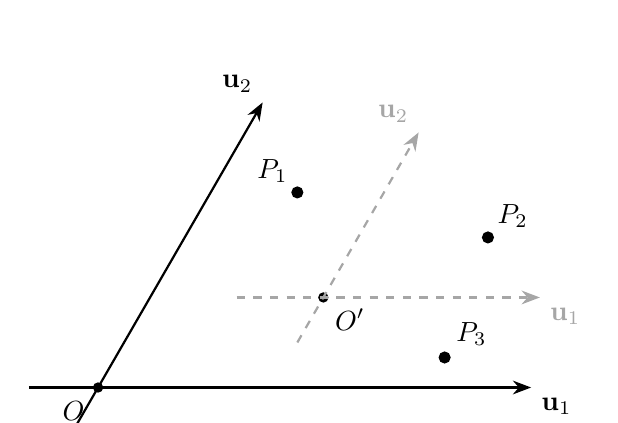
\begin{tikzpicture}[scale=1.1]
  \coordinate (O) at (0, 0);
  \coordinate (U1) at (1, 0);
  \coordinate (U2) at (60:1);

  % Old axes S
  \draw[thick, -Stealth] (-0.8, 0) -- (5.0, 0) node[below right] {$\mathbf{u}_1$};
  \draw[thick, -Stealth] ($-0.6*(U2)$) -- ($3.8*(U2)$) node[above left] {$\mathbf{u}_2$};
  \filldraw (O) circle (1.5pt) node[below left=2pt] {$O$};

  % New origin O'
  \coordinate (Op) at ($2.0*(U1) + 1.2*(U2)$);
  \filldraw (Op) circle (1.5pt) node[below right=1pt] {$O'$};
  \draw[thick, dashed, -Stealth, gray!70] ($(Op) - 1.0*(U1)$) -- ($(Op) + 2.5*(U1)$) node[below right] {$\mathbf{u}_1$};
  \draw[thick, dashed, -Stealth, gray!70] ($(Op) - 0.6*(U2)$) -- ($(Op) + 2.2*(U2)$) node[above left] {$\mathbf{u}_2$};

  % Points P1, P2, P3
  \coordinate (P1) at ($1.0*(U1) + 2.6*(U2)$);
  \coordinate (P2) at ($3.5*(U1) + 2.0*(U2)$);
  \coordinate (P3) at ($3.8*(U1) + 0.4*(U2)$);

  \filldraw (P1) circle (1.8pt) node[above left] {$P_1$};
  \filldraw (P2) circle (1.8pt) node[above right] {$P_2$};
  \filldraw (P3) circle (1.8pt) node[above right=1pt] {$P_3$};
\end{tikzpicture}
\caption{平移座標估計}
\label{fig:b4s-2-3}
\end{figure}

\begin{example}[例 2]
設 $S \equiv (O; \mathbf{i}_1, \mathbf{i}_2), S' \equiv (O'; \mathbf{i}_1, \mathbf{i}_2)$，且平移向量為 $\vec{OO'} = (3, -1)_{S_0} = 3\mathbf{i}_1 - \mathbf{i}_2$。求：
\begin{enumerate}[(i)]
  \item $P_1(-5, 2)$ 相關於 $S'$ 之新座標。
  \item $P_2(1, -3)_{S'}$ 相關於 $S_0$ 之座標。
\end{enumerate}
\end{example}

\begin{proof}[解]
可直接由 \eqref{eq:b4s-1-2-2} 及 \eqref{eq:b4s-1-2-3} 式得
\[ P_1 = (-5-3, 2+1)_{S'} = (-8, 3)_{S'} \]
但最好重複 \eqref{eq:b4s-1-2-2} 及 \eqref{eq:b4s-1-2-3} 式直截的導引過程：
\begin{enumerate}[(i)]
  \item $\vec{O'P_1} = \vec{OP_1} - \vec{OO'} = (-5\mathbf{i}_1 + 2\mathbf{i}_2) - (3\mathbf{i}_1 - \mathbf{i}_2) = (-5-3)\mathbf{i}_1 + (2+1)\mathbf{i}_2 = -8\mathbf{i}_1 + 3\mathbf{i}_2$。故 $P_1 = (-8, 3)_{S'}$。
  \item $\vec{OP_2} = \vec{OO'} + \vec{O'P_2} = (3\mathbf{i}_1 - \mathbf{i}_2) + (\mathbf{i}_1 - 3\mathbf{i}_2) = 4\mathbf{i}_1 - 4\mathbf{i}_2$。故 $P_2 = (4, -4)_{S_0}$。
\end{enumerate}
\end{proof}

\subsubsection*{作業 5}
求：
\begin{enumerate}[(i)]
  \item $P_1(-1, -1)_{S_0}$ 的 $S'$---座標。
  \item $P_2(2, 4)_{S'}$ 的 $S_0$---座標。
\end{enumerate}
並繪圖標出 $P_1$ 及 $P_2$ 之位置，以視察法檢驗 (i)，(ii) 的結果。

\subsubsection*{$\ddagger$ 乙、一般性的座標變換}

座標變換當然不是單純由平移可以概括的。

給定兩種座標系 $S \equiv (O; \mathbf{u}_1, \mathbf{u}_2), S' \equiv (O'; \mathbf{u}_1', \mathbf{u}_2')$，兩種基底間的關係可表成
\begin{align}
\mathbf{u}_1' &= a_{11} \mathbf{u}_1 + a_{12} \mathbf{u}_2 \label{eq:b4s-1-2-4} \\
\mathbf{u}_2' &= a_{21} \mathbf{u}_1 + a_{22} \mathbf{u}_2 \nonumber
\end{align}
而兩基準點的相關位置則可寫成
\begin{equation}
\vec{OO'} = b_1 \mathbf{u}_1 + b_2 \mathbf{u}_2 \label{eq:b4s-1-2-4p}
\end{equation}

\begin{figure}[H]
\centering
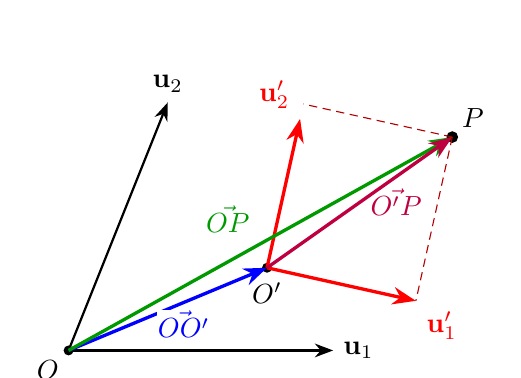
\begin{tikzpicture}[scale=1.05]
  % Old coordinate system S = (O; u1, u2)
  \coordinate (O) at (0, 0);
  \coordinate (U1) at (2.2, 0);
  \coordinate (U2) at (0.8, 2.0);
  \draw[thick, -Stealth] (O) -- ++(3.2, 0) node[right] {$\mathbf{u}_1$};
  \draw[thick, -Stealth] (O) -- ++(1.2, 3.0) node[above] {$\mathbf{u}_2$};
  \filldraw (O) circle (1.5pt) node[below left] {$O$};

  % New origin O' and system S' = (O'; u1', u2')
  \coordinate (Op) at (2.4, 1.0);
  \coordinate (U1p) at (1.8, -0.4);
  \coordinate (U2p) at (0.4, 1.8);
  \filldraw (Op) circle (1.5pt) node[below=2pt] {$O'$};
  \draw[very thick, -Stealth, blue] (O) -- (Op) node[pos=0.58, below=2pt, fill=white, inner sep=0.5pt] {$\vec{OO'}$};

  \draw[very thick, -Stealth, red] (Op) -- ++(U1p) node[below right] {$\mathbf{u}_1'$};
  \draw[very thick, -Stealth, red] (Op) -- ++(U2p) node[above left] {$\mathbf{u}_2'$};

  % Point P
  \coordinate (P) at ($(Op) + 1.0*(U1p) + 1.1*(U2p)$);
  \filldraw (P) circle (1.8pt) node[above right] {$P$};

  % Vectors OP and O'P
  \draw[very thick, -Stealth, green!60!black] (O) -- (P) node[midway, above left] {$\vec{OP}$};
  \draw[very thick, -Stealth, purple] (Op) -- (P) node[midway, right] {$\vec{O'P}$};

  % Dashed projections for P onto S'
  \draw[densely dashed, red!70!black] (P) -- ($(Op) + 1.0*(U1p)$);
  \draw[densely dashed, red!70!black] (P) -- ($(Op) + 1.1*(U2p)$);
\end{tikzpicture}
\caption{一般座標變換}
\label{fig:b4s-2-4}
\end{figure}

欲求一點 $P$ 的兩種座標 $(x_1, x_2)_S$ 與 $(x_1', x_2')_{S'}$ 間的關係。與直線的情形一樣，我們分析 $\vec{OP}$ 的兩種向量座標表示後，再比較係數如下：
\begin{align*}
x_1 \mathbf{u}_1 + x_2 \mathbf{u}_2 &= \vec{OP} = \vec{OO'} + \vec{O'P} \\
&= (b_1 \mathbf{u}_1 + b_2 \mathbf{u}_2) + (x_1' \mathbf{u}_1' + x_2' \mathbf{u}_2') \\
&= (b_1 \mathbf{u}_1 + b_2 \mathbf{u}_2) + [x_1' (a_{11}\mathbf{u}_1 + a_{12}\mathbf{u}_2) + x_2' (a_{21}\mathbf{u}_1 + a_{22}\mathbf{u}_2)] \\
&= (a_{11}x_1' + a_{21}x_2' + b_1)\mathbf{u}_1 + (a_{12}x_1' + a_{22}x_2' + b_2)\mathbf{u}_2
\end{align*}
故得（由第三冊第五章命題 1）
\begin{equation}
\begin{cases}
x_1 = a_{11} x_1' + a_{21} x_2' + b_1 \\
x_2 = a_{12} x_1' + a_{22} x_2' + b_2
\end{cases} \label{eq:b4s-1-2-5}
\end{equation}
這樣一個類似於 § I-1 中 (3) 式的聯立式告訴了我們：如果已知兩種座標系的關係如 \eqref{eq:b4s-1-2-4} 及 \eqref{eq:b4s-1-2-4p}，其中新座標系基底 $\mathbf{u}_1', \mathbf{u}_2'$ 與新基準點 $O'$ 對於舊基準點 $O$ 相對位置，都藉用舊座標系的基底表示如 \eqref{eq:b4s-1-2-5}。也就是說知道了新座標 $(x_1', x_2')_{S'}$，便可以求到舊座標 $(x_1, x_2)_S$。

但是很多時候，我們的需要正好反了過來，亦卽要從舊座標 $(x_1, x_2)_S$ 求得新座標 $(x_1', x_2')_{S'}$，這時我們可以就 \eqref{eq:b4s-1-2-5} 式解出 $(x_1', x_2')$。第一冊第四章二元一次聯立方程式的解法告訴了我們：若取
\[ \Delta = \begin{vmatrix} a_{11} & a_{21} \\ a_{12} & a_{22} \end{vmatrix} = a_{11}a_{22} - a_{12}a_{21} \]
則 $\Delta \neq 0$（為什麼？參考作業 8），且有
\begin{equation}
\begin{cases}
x_1' = \dfrac{a_{22}(x_1 - b_1) - a_{21}(x_2 - b_2)}{\Delta} \\ \noalign{\vskip 1em}
x_2' = \dfrac{-a_{12}(x_1 - b_1) + a_{11}(x_2 - b_2)}{\Delta}
\end{cases} \label{eq:b4s-1-2-6}
\end{equation}
以下諸例的解法著重於舉例再說明 \eqref{eq:b4s-1-2-5} 及 \eqref{eq:b4s-1-2-6} 式的導引過程，而不採取直接代入公式的方式。

\begin{example}[論例 1]
在第三冊第四章講座標幾何，介紹一般座標系時，我們將後者的基底根據原有的正交座標系，表出其向量座標成分，如 § 4-1，例 1，並由繪圖法，比照出相關於此二座標系諸點的新舊座標。用本冊的符號可以把第三冊 § 4-1 例 1 重述如下：

根據已給座標系 $(O; \mathbf{i}_1, \mathbf{i}_2)$ 有二向量 $\mathbf{u}_1, \mathbf{u}_2$：
\[ \mathbf{u}_1 = \vec{OE}_1 = (0, -1), \qquad \mathbf{u}_2 = \vec{OE}_2 = (1, 1) \]
由圖 \ref{fig:b4s-2-5} 可知 $O, E_1, E_2$ 不共線，故 $S \equiv (O; \mathbf{u}_1, \mathbf{u}_2)$ 構成一座標系。今相關於 $(O; \mathbf{i}_1, \mathbf{i}_2)$ 有四點 $A(2, 1), B(-1, 1), C(-1, 0), D(2, 5)$，則這些點相關於新座標系 $(O; \mathbf{u}_1, \mathbf{u}_2)$ 之座標為
\[ A = (1, 2)_S, \quad B = (-2, -1)_S, \quad C = (-1, -1)_S, \quad D = (-3, 2)_S \]
而二基底 $\mathbf{u}_1$ 與 $\mathbf{u}_2$ 相關於 $S$ 的座標成分為 $\mathbf{u}_1 = (1, 0)_S, \mathbf{u}_2 = (0, 1)_S$。

以下則要用本段講的來算新舊座標的變換。因原正交座標系為自然座標系，可記為 $S_0 \equiv (O; \mathbf{i}_1, \mathbf{i}_2)$，而新座標系，則記為 $S \equiv (O; \mathbf{u}_1, \mathbf{u}_2)$，注意此時 $S_0$ 與 $S$ 的原點合一，所以 $\vec{OO'} = \mathbf{0} = 0\mathbf{i}_1 + 0\mathbf{i}_2$。

考慮平面上兩點 $A, A'$。我們要看如何由 $A = (2, 1)_{S_0}$ 得出 $A = (1, 2)_S$ 以及由 $A' = (2, 2)_S$ 得出 $A' = (2, 0)_{S_0}$。
\end{example}

\begin{figure}[H]
\centering
\begin{tikzpicture}[scale=0.8]
  % Dual Grid
  % 1. S0 Cartesian grid
  \draw[very thin, gray!30] (-2.5, -2.5) grid (3.5, 5.5);

  % 2. S affine grid: lines parallel to u2 = (1,1)
  \begin{scope}
    \clip (-2.5, -2.5) rectangle (3.5, 5.5);
    \foreach \k in {-7,-6,-5,-4,-3,-2,-1,0,1,2,3,4,5,6} {
      \draw[very thin, blue!20, dotted] (-2.5, {-2.5 - \k}) -- (3.5, {3.5 - \k});
    }
  \end{scope}
  % lines parallel to u1 = (0,-1) are already the vertical grid lines x = k!

  % Axes S0
  \draw[thick, -Stealth] (-2.5, 0) -- (3.8, 0) node[right] {$\mathbf{i}_1$};
  \draw[thick, -Stealth] (0, -2.5) -- (0, 5.8) node[above] {$\mathbf{i}_2$};
  \filldraw (0, 0) circle (1.5pt) node[below left] {$O$};

  % Base vectors u1 and u2
  \draw[very thick, -Stealth, blue] (0, 0) -- (0, -1) node[left=3pt, fill=white, inner sep=1pt] {$E_1(\mathbf{u}_1)$};
  \draw[very thick, -Stealth, blue] (0, 0) -- (1, 1) node[above left=2pt, fill=white, inner sep=1pt] {$E_2(\mathbf{u}_2)$};

  % Points
  \filldraw (2, 1) circle (2pt) node[right=2pt] {$A(2, 1)_{S_0} = (1, 2)_S$};
  \filldraw (-1, 1) circle (2pt) node[above left=1pt] {$B(-1, 1)$};
  \filldraw (-1, 0) circle (2pt) node[below left=1pt] {$C(-1, 0)$};
  \filldraw (2, 5) circle (2pt) node[above right=1pt] {$D(2, 5) = (-3, 2)_S$};
  \filldraw (2, 0) circle (2pt) node[below right=1pt] {$A'(2, 0)_{S_0} = (2, 2)_S$};

  % Unit scale indicator
  \draw[|<->|] (3.2, -1.8) -- (4.2, -1.8) node[midway, below] {\footnotesize 單位長};
\end{tikzpicture}
\caption{新舊座標系點的對照}
\label{fig:b4s-2-5}
\end{figure}

由假設，基底關係為：
\begin{align*}
\mathbf{u}_1 &= 0 \cdot \mathbf{i}_1 - 1 \cdot \mathbf{i}_2 \\
\mathbf{u}_2 &= 1 \cdot \mathbf{i}_1 + 1 \cdot \mathbf{i}_2
\end{align*}
\begin{proof}[解]
\begin{enumerate}[(i)]
  \item 設 $A$ 點相對於 $S$ 的座標為 $(x_1', x_2')_S$，則
  \begin{align*}
  2\mathbf{i}_1 + 1\mathbf{i}_2 &= \vec{OA} = x_1' \mathbf{u}_1 + x_2' \mathbf{u}_2 \\
  &= x_1'(0\mathbf{i}_1 - 1\mathbf{i}_2) + x_2'(1\mathbf{i}_1 + 1\mathbf{i}_2) \\
  &= x_2'\mathbf{i}_1 + (-x_1' + x_2')\mathbf{i}_2
  \end{align*}
  因 $\mathbf{i}_1$ 與 $\mathbf{i}_2$ 線性無關，故有
  \[ \begin{cases} x_2' = 2 \\ -x_1' + x_2' = 1 \end{cases} \implies x_1' = 1, \; x_2' = 2 \]
  故 $A = (1, 2)_S$。
  \item 設 $A'$ 點相對於 $S_0$ 的座標為 $(x_1, x_2)$，則
  \begin{align*}
  x_1\mathbf{i}_1 + x_2\mathbf{i}_2 &= \vec{OA'} = 2\mathbf{u}_1 + 2\mathbf{u}_2 \\
  &= 2(0\mathbf{i}_1 - 1\mathbf{i}_2) + 2(1\mathbf{i}_1 + 1\mathbf{i}_2) \\
  &= (0 + 2)\mathbf{i}_1 + (-2 + 2)\mathbf{i}_2 = 2\mathbf{i}_1 + 0\mathbf{i}_2
  \end{align*}
  故 $x_1 = 2, x_2 = 0$，卽 $A' = (2, 0)_{S_0}$。
\end{enumerate}
\end{proof}

\begin{figure}[H]
\centering
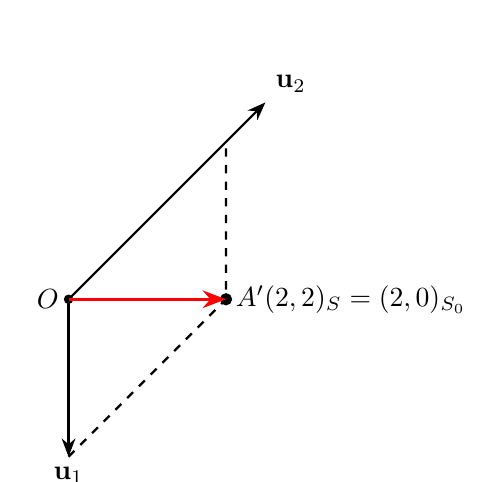
\begin{tikzpicture}[scale=1.0]
  \draw[thick, -Stealth] (0, 0) -- (0, -2) node[below] {$\mathbf{u}_1$};
  \draw[thick, -Stealth] (0, 0) -- (2.5, 2.5) node[above right] {$\mathbf{u}_2$};
  \filldraw (0, 0) circle (1.5pt) node[left] {$O$};

  \coordinate (Ap) at (2, 0);
  \filldraw (Ap) circle (2pt) node[right] {$A'(2, 2)_S = (2, 0)_{S_0}$};
  \draw[thick, dashed] (0, -2) -- (2, 0) -- (2, 2);
  \draw[very thick, -Stealth, red] (0, 0) -- (Ap);
\end{tikzpicture}
\caption{$A'$ 在新座標系下之向量分解}
\label{fig:b4s-2-6}
\end{figure}

\subsubsection*{作業 6}
\begin{enumerate}[(i)]
  \item 在論例 1 中，求點 $B = (-1, 1), C = (-1, 0), D = (2, 5)$ 相關於座標系 $S$ 的座標。
  \item 在論例 1 中，求點 $B' = (1, -3)_S, C' = (-1, 3)_S, D' = (-3, -2)_S$ 相關於 $S_0$ 的座標。
\end{enumerate}

第三冊所比較的兩個不同座標系有一個特點，就是具有共同的原點，現在我們來看若原點改變，結果如何。

\begin{example}[例 3]
設 $S' \equiv (O'; \mathbf{u}_1, \mathbf{u}_2)$ 其基底與上論例相同，而 $\vec{OO'} = (3, -1)_{S_0}$。試求 $A(2, 1)$ 對 $S'$ 的座標及 $A'(2, 2)_{S'}$ 對 $S_0$ 的座標。
\end{example}

\begin{proof}[解]
設 $A = (x_1', x_2')_{S'}, A' = (x_1, x_2)_{S_0}$，則有
\begin{align*}
2\mathbf{i}_1 + 1\mathbf{i}_2 &= \vec{OA} = \vec{OO'} + \vec{O'A} \\
&= (3\mathbf{i}_1 - \mathbf{i}_2) + [x_1'(0\mathbf{i}_1 - 1\mathbf{i}_2) + x_2'(1\mathbf{i}_1 + 1\mathbf{i}_2)] \quad \text{〔由基底間的關係〕} \\
&= (3 + x_2')\mathbf{i}_1 + (-1 - x_1' + x_2')\mathbf{i}_2
\end{align*}
而有
\[ \begin{cases} 3 + x_2' = 2 \\ -1 - x_1' + x_2' = 1 \end{cases} \implies x_2' = -1, \; x_1' = -3 \]
故 $A = (2, 1) = (-3, -1)_{S'}$。

又
\begin{align*}
x_1\mathbf{i}_1 + x_2\mathbf{i}_2 &= \vec{OA'} = \vec{OO'} + \vec{O'A'} \\
&= (3\mathbf{i}_1 - \mathbf{i}_2) + [2(0\mathbf{i}_1 - 1\mathbf{i}_2) + 2(1\mathbf{i}_1 + 1\mathbf{i}_2)] \quad \text{〔由基底間的關係〕} \\
&= (3 + 2)\mathbf{i}_1 + (-1 - 2 + 2)\mathbf{i}_2 = 5\mathbf{i}_1 - 1\mathbf{i}_2
\end{align*}
$\therefore x_1 = 5, x_2 = -1$。故 $A' = (2, 2)_{S'} = (5, -1)_{S_0}$。
\end{proof}

\subsubsection*{作業 7}
取 $S'$ 如例 3，仿例 3 求作業 6 中各題。

\subsubsection*{作業 8}
試解釋在 \eqref{eq:b4s-1-2-6} 式中 $\Delta \neq 0$（提示：參考第三冊 § 3-7 行列式與面積）。

總結本節結果，可得：

\begin{theorem}[定理 2]
給定平面上兩個座標系 $S \equiv (O; \mathbf{u}_1, \mathbf{u}_2)$ 及 $S' \equiv (O'; \mathbf{u}_1', \mathbf{u}_2')$ 如果
\begin{align*}
\mathbf{u}_1' &= a_{11}\mathbf{u}_1 + a_{12}\mathbf{u}_2 \\
\mathbf{u}_2' &= a_{21}\mathbf{u}_1 + a_{22}\mathbf{u}_2
\end{align*}
而且 $\vec{OO'} = b_1\mathbf{u}_1 + b_2\mathbf{u}_2$，則
\begin{equation}
\begin{cases}
x_1 = a_{11}x_1' + a_{21}x_2' + b_1 \\
x_2 = a_{12}x_1' + a_{22}x_2' + b_2
\end{cases} \label{eq:b4s-1-2-thm2-5}
\end{equation}
或
\begin{equation}
\begin{cases}
x_1' = \dfrac{a_{22}(x_1 - b_1) - a_{21}(x_2 - b_2)}{\Delta} \\ \noalign{\vskip 1em}
x_2' = \dfrac{-a_{12}(x_1 - b_1) + a_{11}(x_2 - b_2)}{\Delta}
\end{cases} \label{eq:b4s-1-2-thm2-6}
\end{equation}
其中 $\Delta = a_{11}a_{22} - a_{12}a_{21}$。
\end{theorem}

注意比較 \eqref{eq:b4s-1-2-4} 與 \eqref{eq:b4s-1-2-thm2-5} 式之一次部份：除 $a_{12}$ 與 $a_{21}$ 互調外，其餘相同。但注意 \eqref{eq:b4s-1-2-4} 式將 $\mathbf{u}_1'$ 及 $\mathbf{u}_2'$ 以 $\mathbf{u}_1$ 及 $\mathbf{u}_2$ 表示，\eqref{eq:b4s-1-2-thm2-5} 式則將 $x_1$ 及 $x_2$ 以 $x_1'$ 及 $x_2'$ 表示。

\vspace{1em}
\noindent\textbf{**【論例 2】（相對性原理）}\phantomsection\label{note:b4s-ch1-p16-lorentz}\footnote{【原書註記/校訂】：原書標註「**【論例 2】（相對性原理）」，依目次「注意 1」規範，「**」表示本節段為選授/進階補充內容。}

平面上有兩同原點座標系 $S_0 \equiv (O; \mathbf{e}_1, \mathbf{e}_2), S \equiv (O; \mathbf{u}_1, \mathbf{u}_2)$，其中 $S_0$ 為正交座標系。設 $(x, t)$ 與 $(x', t')$ 分別為 $S_0$---座標與 $S$---座標，且其座標變換式為
\begin{equation}
\begin{cases}
x' = \dfrac{x - vt}{\sqrt{1 - \dfrac{v^2}{c^2}}} \\[1.5em]
t' = \dfrac{-\dfrac{v}{c^2}x + t}{\sqrt{1 - \dfrac{v^2}{c^2}}}
\end{cases} \label{eq:b4s-lorentz-1}
\end{equation}
（稱羅倫茲（Lorentz）變換）其中 $c, v$ 皆為常數，求得兩組基底的關係應為（據 § I-2 \eqref{eq:b4s-1-2-4} 及 \eqref{eq:b4s-1-2-5} 式）
\begin{align*}
\mathbf{u}_1 &= \frac{\mathbf{e}_1 + \dfrac{v}{c^2}\mathbf{e}_2}{\sqrt{1 - \dfrac{v^2}{c^2}}} \\
\mathbf{u}_2 &= \frac{v\mathbf{e}_1 + \mathbf{e}_2}{\sqrt{1 - \dfrac{v^2}{c^2}}}
\end{align*}

今取平面上一點 $P$ 對一個靜坐在臺北站的觀測者甲看來 $P$ 可當作在 $t$ 時刻自臺北沿縱貫路南下 $x$ 公里處發生的一個事件，則相對論告訴我們，若有另一觀測者乙以等速度 $v$ 離甲（沿縱貫路）南去時，則剛才那一事件從乙看來應是 $t'$ 時刻在乙之南 $x'$ 公里處發生的事件。（$x'$ 為負時，代表事件發生在乙之北）。而這 $x', t'$ 與 $x, t$ 的關係由上述羅倫茲變換式給定，其中 $c$ 代表光速。

\begin{figure}[H]
\centering
\begin{tikzpicture}[scale=1.1]
  \draw[thick, -Stealth] (-0.5, 0) -- (4.5, 0) node[right] {$x$ ($\mathbf{e}_1$)};
  \draw[thick, -Stealth] (0, -0.5) -- (0, 4.1) node[above] {$t$ ($\mathbf{e}_2$)};
  \filldraw (0, 0) circle (1.5pt) node[below left] {$O$};

  % u1 (x') and u2 (t') axes (tilted)
  \draw[very thick, -Stealth, blue] (0, 0) -- (4.0, 1.4) node[right] {$x'$ ($\mathbf{u}_1$)};
  \draw[very thick, -Stealth, blue] (0, 0) -- (1.4, 4.0) node[above] {$t'$ ($\mathbf{u}_2$)};

  % Simultaneous line in S' (parallel to x' axis, slope 0.35)
  \draw[thick, dashed, green!60!black] (0.2, 1.27) -- (4.2, 2.67) node[right] {\small $t' = \text{常數}$};

  % Events P1 and P2 on the simultaneous line
  \coordinate (P1) at (3.3, 2.355);
  \coordinate (P2) at (1.8, 1.83);
  \filldraw (P1) circle (2pt) node[above=3pt, fill=white, inner sep=1pt] {$P_1(x_1', t')_S$};
  \filldraw (P2) circle (2pt) node[below right=2pt, fill=white, inner sep=1pt] {$P_2(x_2', t')_S$};

  % Projections to t-axis showing t1 != t2
  \draw[dotted, gray] (P1) -- (0, 2.355) node[left] {\footnotesize $t_1$};
  \draw[dotted, gray] (P2) -- (0, 1.83) node[left] {\footnotesize $t_2$};
\end{tikzpicture}
\caption{羅倫茲變換時空圖}
\label{fig:b4s-2-7}
\end{figure}

相對論提出了幾點“新”的看法：
\begin{enumerate}[(i)]
  \item 它告訴我們傳統的所謂「同時」這一概念不是絕對的，而是依賴於觀測者的。解釋如下：取兩事件 $P_1(x_1', t')_S$ 與 $P_2(x_2', t')_S$。就是說，這兩事件從 $S$ 的乙觀測者看來，都發生在 $t'$ 時刻，是“同時的”，但根據變換式，這兩事件對 $S_0$ 的甲觀測者看來，則分別發生於不同時刻：
  \[ t_1 = \frac{\dfrac{v}{c^2}x_1' + t'}{\sqrt{1 - \dfrac{v^2}{c^2}}}, \qquad t_2 = \frac{\dfrac{v}{c^2}x_2' + t'}{\sqrt{1 - \dfrac{v^2}{c^2}}} \]
  兩事件發生的時差（對甲而言）為
  \[ t_1 - t_2 = \frac{\dfrac{v}{c^2}(x_1' - x_2')}{\sqrt{1 - \dfrac{v^2}{c^2}}} \]
  亦卽對甲而言，這兩事件並不“同時”。因此“同時”是一個相對性的概念。

  但注意當 $v$ 不是大到可與光速比較時，這時差非常細微，可以忽略不計。例如在日常或傳統的力學，如星體，砲彈，火箭等的相對運動下，「同時」仍有它逼近絕對性的意義。

  \item 設有一巨尺，其對靜止的甲看來長度為 $l$，將其自臺北站往南平放於縱貫路上，尺的兩端分別設一藍燈與紅燈，使其持續發光，則發藍光與發紅光為兩整串的事件，在 $(x, t)$ 平面上分別描出
  \[ x = 0, \qquad x = l \]
  兩條直線（半射線）。

  今乙觀測者要測此巨尺的長度，設他觀測的時刻為 $t'$，則 $t'$ 時刻他“看到的”藍光與紅光的位置 $x_1', x_2'$ 其差距 $x_2' - x_1'$ 卽為他所測得的尺長 $l'$。

  由 \eqref{eq:b4s-lorentz-1} 式，解得其 $x, t$ 表為 $x', t'$ 的座標變換式為（作業 9）：
  \begin{equation}
  \begin{cases}
  x = \dfrac{x' + vt'}{\sqrt{1 - \dfrac{v^2}{c^2}}} \\[1.5em]
  t = \dfrac{\dfrac{v}{c^2}x' + t'}{\sqrt{1 - \dfrac{v^2}{c^2}}}
  \end{cases} \label{eq:b4s-lorentz-2}
  \end{equation}
  其相應的 $S_0$ 的第一座標為：$x_1 = 0, x_2 = l$。

  \begin{figure}[H]
  \centering
  \begin{tikzpicture}[scale=1.05]
    \draw[thick, -Stealth] (-0.5, 0) -- (4.2, 0) node[right] {$x$};
    \draw[thick, -Stealth] (0, -0.5) -- (0, 4.3) node[above] {$t$};
    \filldraw (0, 0) circle (1.5pt) node[below left] {$O$};

    % World lines x=0 and x=l
    \draw[very thick, blue] (0, 0) -- (0, 3.7) node[left=3pt] {\small $x=0$ (藍光)};
    \draw[very thick, red] (2.6, 0) -- (2.6, 3.7) node[above=2pt] {\small $x=l$ (紅光)};
    \draw[|<->|] (0, -0.45) -- (2.6, -0.45) node[midway, fill=white, inner sep=1pt] {\small $l$};

    % Line of constant t'
    \draw[thick, dashed, green!60!black] (-0.5, 0.8) -- (3.8, 2.2) node[right] {\small $t' = \text{常數}$};
    \filldraw (0, 0.96) circle (2pt) node[below left=2pt] {$x_1'$};
    \filldraw (2.6, 1.8) circle (2pt) node[below right=2pt] {$x_2'$};
    \draw[|<->|, purple] ($(0, 0.96) + (-0.1, 0.25)$) -- ($(2.6, 1.8) + (-0.1, 0.25)$) node[midway, above left] {\small $l'$};
  \end{tikzpicture}
  \caption{長度測量與尺縮效應}
  \label{fig:b4s-2-8}
  \end{figure}

  由 \eqref{eq:b4s-lorentz-2} 中第一式：
  \[ x_1 = \frac{x_1' + vt'}{\sqrt{1 - \dfrac{v^2}{c^2}}} = 0 \implies x_1' = -vt' \]
  \[ x_2 = \frac{x_2' + vt'}{\sqrt{1 - \dfrac{v^2}{c^2}}} = l \implies x_2' + vt' = l\sqrt{1 - \frac{v^2}{c^2}} \implies x_2' = l\sqrt{1 - \frac{v^2}{c^2}} - vt' \]
  故
  \[ l' = x_2' - x_1' = l\sqrt{1 - \frac{v^2}{c^2}} \]
  故從乙看來，該尺竟然自 $l$ 壓縮了 $\sqrt{1 - \dfrac{v^2}{c^2}}$ 倍，卽得尺長 $l\sqrt{1 - \dfrac{v^2}{c^2}}$。這就稱為「長度的壓縮性」（或空間的壓縮性）。
\end{enumerate}

\subsubsection*{作業 9}
試由 \eqref{eq:b4s-lorentz-1} 式解得 \eqref{eq:b4s-lorentz-2} 式。

\subsubsection*{作業 10}
如果兩觀測者的相對速度與光速 $c$ 相較甚小，則傳統力學適用（此時 $\dfrac{v}{c}$ 與 $\dfrac{v^2}{c^2}$ 皆甚小）。解釋此時 \eqref{eq:b4s-lorentz-1} 式的意義。

\subsubsection*{作業 11}
甲觀測系統的尺度，由乙看來壓縮了 $\sqrt{1 - \dfrac{v^2}{c^2}}$ 倍，反過來乙的尺度甲看起來應為伸漲或壓縮？其漲縮率為何？

\subsubsection*{習題 1-2}
\begin{enumerate}
  \item 在平面上取一自然座標系 $S_0 \equiv (O; \mathbf{i}_1, \mathbf{i}_2)$，假設有一點 $P$ 用此座標系表示時 $P = (1, 0)$。令
  \begin{enumerate}[a.]
    \item $A = (1, 1), B = (-1, 1)$
    \item $A = (0, 1), B = (\frac{1}{2}, \frac{1}{2})$
    \item $A = (\frac{1}{2}, 5), B = (-\frac{3}{5}, -6)$
  \end{enumerate}
  問：
  \begin{enumerate}[(i)]
    \item 上述各種情形中 $(O; \vec{OA}, \vec{OB})$ 是不是可以形成一座標系？
    \item 上述各種情形中 $(P; \vec{PA}, \vec{PB})$ 可不可以成為一個座標系？
  \end{enumerate}

  \item 設 $S \equiv (O; \mathbf{u}_1, \mathbf{u}_2)$ 為平面 $\mathbb{R}^2$ 上的一個座標系，現在有 $\mathbb{R}^2$ 上的三點 $O', A, B$ 用此座標系表示為：$O' = (1, 1)_S, A = (\sqrt{2}, 5)_S, B = (4, -1)_S$。令 $\mathbf{u}_1' = \vec{O'A}, \mathbf{u}_2' = \vec{O'B}$，問：
  \begin{enumerate}[(i)]
    \item $S' \equiv (O'; \mathbf{u}_1', \mathbf{u}_2')$ 是不是可成為一個座標系？
    \item 如果 $S' \equiv (O'; \mathbf{u}_1', \mathbf{u}_2')$ 是個座標系，則由 $S$ 變換成 $S'$ 的座標變換如何表示？
  \end{enumerate}

  \item 把地球表面看成一個平面，以臺北做原點 $O$，以向東 $1$ 公里的向量 $\mathbf{e}_1$ 及向北 $1$ 公里的向量 $\mathbf{e}_2$ 為基底得一座標系。香港因為目前是英國屬地，以英制的哩為單位，故在香港 $O'$ 可以拿向東 $1$ 哩的向量 $\mathbf{e}_1'$ 及向北 $1$ 哩的向量 $\mathbf{e}_2'$ 做基底得另一座標系，現已知香港是在臺北的西方 $800$ 公里，如果有一艘船在海上，由臺北的座標來看，它的位置是在 $(-300, 200)$ 處。由香港做原點的座標系來看，它的位置應該如何表示？（$1$ 哩 $= 1.6093$ 公里）。

  \item 如果有一天，我國收回了香港，當然香港的度量衡也改為公制了。香港的里程也就以公里來計算，則上題的答案如何？

  \item 有一同學在操場上沿一直線跑步，現假設操場為一平面，以公尺為長度單位，在他起跑點 $O$ 做一座標系 $(O; \mathbf{e}_1, \mathbf{e}_2)$。他跑步的速度如用向量表示為每秒鐘 $\mathbf{v} = 3\mathbf{e}_1 + 4\mathbf{e}_2$。在他跑步的每一瞬間用他當時的位置做原點，用同樣的 $\mathbf{e}_1, \mathbf{e}_2$ 做基底可得一座標系，如此我們就得到了一個在操場上移動的座標系，現操場上有一個國旗桿，它的位置若用跑到 $10$ 秒時的座標系來表示是 $(20, 30)$ 問用跑到 $25$ 秒時的座標系應該如何表示？兩個座標系之間如何變換？

  \item 設有一火車在軌道上沿一直線作等速運動，設在時刻 $t$ 火車的位置為 $O_t$，我們固定兩個方向 $\mathbf{e}_1, \mathbf{e}_2$ 作基底，則在任意時刻 $t$，均有一座標系 $(O_t; \mathbf{e}_1, \mathbf{e}_2) \equiv S_t$。因火車在每一秒鐘均走一固定的向量 $\mathbf{v}$，設 $\mathbf{v} = 5\mathbf{e}_1$，當時刻 $t = 0$ 時，我們看見有一房屋，對 $S_0$ 是在 $(0, 2)$ 的位置，試問在時刻 $t$ 時，相對於 $S_t$ 座標系，該房屋的座標應為多少？（讀者會發現在每個時刻 $t$，房屋所對應於 $S_t$ 的座標均不同，此卽何以我們在車輛中感覺到車外的房屋一直在動的原因）。
\end{enumerate}
% =========================================================================
% § I-3 平面上的線性映射
% =========================================================================
\subsection{平面上的線性映射}
\label{sec:b4s-1-3}

本段將固定採用自然座標系 $S_0$。

\subsubsection*{甲、線性映射的意義}

上節（§ I-2）座標變換的式子 \eqref{eq:b4s-1-2-5}
\begin{align*}
x_1 &= a_{11}x_1' + a_{21}x_2' + b_1 \\
x_2 &= a_{12}x_1' + a_{22}x_2' + b_2
\end{align*}
及 § I-1 的 (3)（或 (3')）
\[ x = ax' + b \]
使我們想起實數系 $\mathbb{R} = \mathbb{R}^1$〔註〕的一次變換
\begin{equation}
y = ax + b \label{eq:b4s-1-3-1}
\end{equation}
亦卽考慮一次函數 $f: \mathbb{R}^1 \to \mathbb{R}^1$ 其中
\begin{equation}
f(x) = ax + b \label{eq:b4s-1-3-2}
\end{equation}
這種函數在自然或人文現象的各種函數關係中最是單純，我們已從第三冊學得它可以圖解如下：

\begin{figure}[H]
\centering
\begin{tikzpicture}[scale=1.0]
  \draw[thick, -Stealth] (-1, 0) -- (4, 0) node[right] {$x$};
  \draw[thick, -Stealth] (0, -1) -- (0, 3.5) node[above] {$y$};
  \filldraw (0, 0) circle (1.5pt) node[below left] {$O$};

  \draw[very thick, blue] (-0.5, 0.5) -- (3.5, 3.1) node[right] {$y = ax + b$};
  \filldraw (0, 0.83) circle (1.5pt) node[left=3pt] {$b$};
  \node[anchor=west] at (1.5, 1.2) {\small $a$ 代表這直線的斜率};
  \node[anchor=west] at (1.5, 0.7) {\small $b$ 代表 $y$ 截距};
\end{tikzpicture}
\caption{一次函數之圖形}
\label{fig:b4s-1-3-1}
\end{figure}

〔註〕實數軸上點變動的自由度為 $1$，我們把實數系看成是 $1$ 維的，所以寫成 $\mathbb{R}^1$。平面上點變動的自由度為 $2$，我們把平面看成 $\mathbb{R} \times \mathbb{R}$，將寫成 $\mathbb{R}^2$。

現在將 \eqref{eq:b4s-1-3-1} 式寫成
\begin{equation}
\begin{cases}
y_1 = a_{11}x_1 + a_{21}x_2 + b_1 \\
y_2 = a_{12}x_1 + a_{22}x_2 + b_2
\end{cases} \label{eq:b4s-1-3-3}
\end{equation}
\eqref{eq:b4s-1-3-3} 式可以看成：兩變量 $y_1$ 與 $y_2$ 相應於兩變量 $x_1$ 及 $x_2$ 的變化關係，就這立場，我們慣以函數稱之。但當我們把 $(x_1, x_2), (y_1, y_2)$ 都看成平面上的點時，我們注重的是平面上點的位置變動的情形，此時慣以映射稱之。〔見章末附註〕

這一節我們特別注重函數的幾何意義，而因 \eqref{eq:b4s-1-3-3} 式所給的函數是一次的，我們先考慮所謂的“線性映射”：

\begin{definition}[定義]
設 $f: \mathbb{R}^2 \to \mathbb{R}^2$ 為一函數，以 $(y_1, y_2)$ 表 $(x_1, x_2)$ 在 $f$ 下之像點，而知存在四實數 $a_{11}, a_{12}, a_{21}, a_{22}$，使得
\begin{equation}
\begin{cases}
y_1 = a_{11}x_1 + a_{21}x_2 \\
y_2 = a_{12}x_1 + a_{22}x_2
\end{cases} \label{eq:b4s-1-3-4}
\end{equation}
對每一點 $(x_1, x_2)$ 都成立，則稱 $f$ 為 $\mathbb{R}^2$ 到 $\mathbb{R}^2$ 的一個線性映射。（注意：$y_1$ 與 $y_2$ 均為 $x_1$ 與 $x_2$ 的一次齊次函數）
\end{definition}

\begin{figure}[H]
\centering
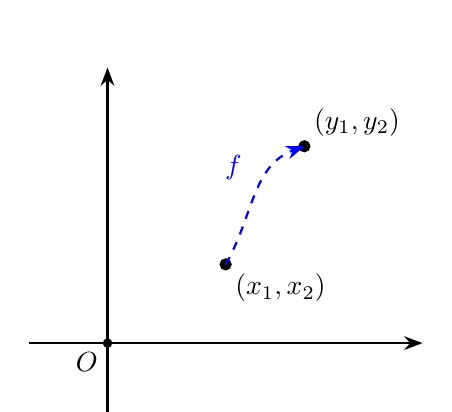
\begin{tikzpicture}[scale=1.0]
  \draw[thick, -Stealth] (-1, 0) -- (4, 0);
  \draw[thick, -Stealth] (0, -1) -- (0, 3.5);
  \filldraw (0, 0) circle (1.5pt) node[below left] {$O$};

  \filldraw (1.5, 1.0) circle (2pt) node[below right] {$(x_1, x_2)$};
  \filldraw (2.5, 2.5) circle (2pt) node[above right] {$(y_1, y_2)$};
  \draw[thick, -Stealth, dashed, blue] (1.5, 1.0) to[out=60, in=200] node[midway, above left=2pt] {$f$} (2.5, 2.5);
\end{tikzpicture}
\caption{線性映射示意圖}
\label{fig:b4s-1-3-2}
\end{figure}

這樣定義得來的線性映射可寫成：
\begin{equation}
f(x_1, x_2) = (a_{11}x_1 + a_{21}x_2, \; a_{12}x_1 + a_{22}x_2) \label{eq:b4s-1-3-5}
\end{equation}

\noindent\textbf{注意}：線性映射是把平面的點移到新的位置，而座標變換的意義則是固定平面上的點，只按照新舊座標間的關係來改寫平面上點的座標表示。當兩座標系之原點合一時，線性映射與座標變換的代數式一樣，兩方面的推論結果可相互轉化來利用，但注意就其自然的意義來看兩者是有著區別的。

\begin{example}[例 4]
已知線性映射 $f$ 由下式給出：
\[ \begin{cases} y_1 = 3x_1 - x_2 \\ y_2 = 2x_1 + x_2 \end{cases} \]
求 $O(0, 0), A(2, 0), B(1, 1), C(0, 2)$ 相應之像點 $O', A', B', C'$ 的座標，又 $A, B, C$ 三點同在一直線上，問 $A', B', C'$ 是否也同在一直線上？
\end{example}

\begin{proof}[解]
計算易知 $f(0, 0) = (0, 0), f(1, 1) = (2, 3), f(2, 0) = (6, 4), f(0, 2) = (-2, 2)$。故 $A' = (6, 4), B' = (2, 3), C' = (-2, 2)$。

檢驗三點 $A', B', C'$ 是否共線的方法很多，由 $\vec{A'B'} = (-4, -1), \vec{B'C'} = (-4, -1)$ 可知共線，或由行列式
\[ \begin{vmatrix} 6 & 4 & 1 \\ 2 & 3 & 1 \\ -2 & 2 & 1 \end{vmatrix} = 0 \]
亦可知（第三冊 § 4-2 論例 3）。
\end{proof}

\subsubsection*{作業 12}
對於自然座標系 $S_0$，四點 $A(-1, -1), B(3, 1), C(1, 5), D(-3, 3)$ 做成一正方形的頂點（為什麼？試先檢驗）。
\begin{enumerate}[(i)]
  \item 求在例 4 的線性映射下，此四點的像點。
  \item 此四像點仍做成一正方形的頂點嗎？或為一矩形？或只得一平行四邊形？甚或僅為一任意四邊形而已？
  \item 試求基底向量的終點的像點，並由像點的座標寫出基底經線性映射後變成的新向量 $\mathbf{u}_1, \mathbf{u}_2$，試問四像點，對應於 $S \equiv (O; \mathbf{u}_1, \mathbf{u}_2)$ 的座標如何？（此題表示一般的線性映射不保持角度也不保持長度）。
\end{enumerate}

\subsubsection*{乙、線性映射的基本性質}

我們已在例 4 中看出在線性映射下原點的像點仍為原點。

線性映射既然是一個把平面上的點指向其像點的函數，自然能把平面上的向量（先看成自原點出發的）指向以原點為起點，以其終點之像點為終點的向量。若 $P$ 為點 $(x_1, x_2)$，$Q$ 表 $P$ 經 $f$ 的像點，則有兩種寫法：$f(P) = Q$ 或 $f(\vec{OP}) = \vec{OQ}$。

也就是說：若 $f: \mathbb{R}^2 \to \mathbb{R}^2$ 為線性映射，則 $f(\vec{OP}) = \vec{OQ}$，其中 $Q$ 為 $P$ 經 $f$ 的像點。我們利用平面的點與自某定點出發以之為終點的向量的一一對應，有時把 $f$ 的定義域 $\mathbb{R}^2$ 中的元素看成點，有時又把 $\mathbb{R}^2$ 的元素看成向量，事實上點的座標與其相應向量的座標成分是一樣的，故為了不同需要可以寫 $f(P) = Q$，亦可寫 $f(\vec{OP}) = \vec{OQ}$。

$\mathbb{R}^2$ 中的元素既然可以看成向量，而向量在本質上是可以不計其起始點的，因此對任給向量 $\mathbf{a}$，$f(\mathbf{a})$ 也就有了一定的意思，卽：$f(\mathbf{a})$ 是以 $\mathbf{a}$ 的始點之像點為始點，$\mathbf{a}$ 終點之像點為終點的向量，稱為向量 $\mathbf{a}$ 的映像。

第三冊 § 5-1 提到空間中自同一點出發的兩個線性無關向量 $\mathbf{a}$ 與 $\mathbf{b}$ 可張出一平面 $P$，而此平面又可依據此二向量為基底，共同始點為原點做成其上的一座標系。設共同出發點為 $O$，則 $P = \{P \mid \vec{OP} = \alpha\mathbf{a} + \beta\mathbf{b}\}$，我們稱向量 $\vec{OP}$ 為 $\mathbf{a}$ 與 $\mathbf{b}$ 的線性組合，此組合的係數卽為此點相關於座標系 $S \equiv (O; \mathbf{a}, \mathbf{b})$ 的座標。

由以上的觀點，甲段所述的線性映射（\eqref{eq:b4s-1-3-4} 式）有一可以不藉座標便能表達的特徵性質，卽：平面上兩向量的線性組合，經線性映射後的映像，為此兩向量的映像的線性組合。

\begin{theorem}[定理 3]
若 $f: \mathbb{R}^2 \to \mathbb{R}^2$ 為一線性映射，則對於任意兩實數 $\alpha, \beta \in \mathbb{R}^1$ 及任意平面上的兩向量 $\mathbf{a}$ 與 $\mathbf{b}$ 總有
\begin{equation}
f(\alpha\mathbf{a} + \beta\mathbf{b}) = \alpha f(\mathbf{a}) + \beta f(\mathbf{b}) \label{eq:b4s-1-3-6}
\end{equation}
（\eqref{eq:b4s-1-3-6} 式的性質，稱為函數 $f$ 的線性條件）。
\end{theorem}

\begin{proof}[證明]
設 $\mathbf{a} = (x_1, x_2), \mathbf{b} = (x_1', x_2')$，則 $\alpha\mathbf{a} + \beta\mathbf{b} = (\alpha x_1 + \beta x_1', \alpha x_2 + \beta x_2')$。故由 \eqref{eq:b4s-1-3-4} 式：
\begin{align*}
f(\alpha\mathbf{a} + \beta\mathbf{b}) &= (a_{11}(\alpha x_1 + \beta x_1') + a_{21}(\alpha x_2 + \beta x_2'), \; a_{12}(\alpha x_1 + \beta x_1') + a_{22}(\alpha x_2 + \beta x_2')) \\
&= \alpha(a_{11}x_1 + a_{21}x_2, a_{12}x_1 + a_{22}x_2) + \beta(a_{11}x_1' + a_{21}x_2', a_{12}x_1' + a_{22}x_2') \\
&= \alpha f(\mathbf{a}) + \beta f(\mathbf{b})
\end{align*}
\end{proof}

\eqref{eq:b4s-1-3-6} 式這一個性質非常基本，特別地：
\begin{enumerate}[(i)]
  \item 取 $\alpha = 1, \beta = 1$，得 $f(\mathbf{a} + \mathbf{b}) = f(\mathbf{a}) + f(\mathbf{b})$（保加法性，圖 \ref{fig:b4s-1-3-3}）。
  \item 取 $\beta = 0$，得 $f(\alpha\mathbf{a}) = \alpha f(\mathbf{a})$（保係數積，圖 \ref{fig:b4s-1-3-4}）。
  \item 取 $\alpha = 0, \beta = 0$，得 $f(\mathbf{0}) = \mathbf{0}$（原點不變）。
  \item 取 $\alpha = 1, \beta = -1$，得 $f(\mathbf{a} - \mathbf{b}) = f(\mathbf{a}) - f(\mathbf{b})$。
\end{enumerate}

\begin{figure}[H]
\centering
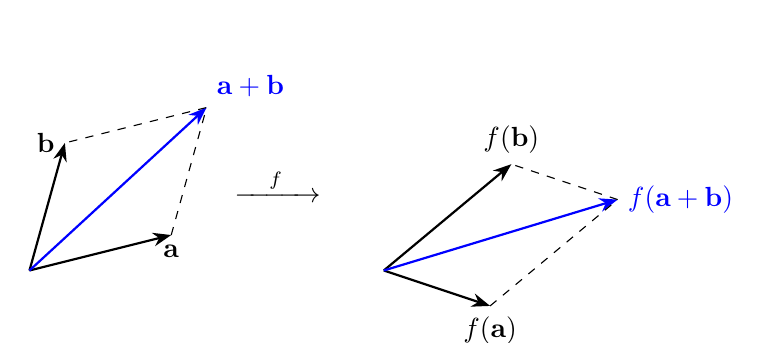
\begin{tikzpicture}[scale=0.9]
  % Addition
  \draw[thick, -Stealth] (0, 0) -- (2, 0.5) node[below] {$\mathbf{a}$};
  \draw[thick, -Stealth] (0, 0) -- (0.5, 1.8) node[left] {$\mathbf{b}$};
  \draw[thick, -Stealth, blue] (0, 0) -- (2.5, 2.3) node[above right] {$\mathbf{a}+\mathbf{b}$};
  \draw[dashed] (2, 0.5) -- (2.5, 2.3) -- (0.5, 1.8);

  \node at (3.5, 1.2) {$\xrightarrow{\quad f \quad}$};

  \begin{scope}[shift={(5, 0)}]
    \draw[thick, -Stealth] (0, 0) -- (1.5, -0.5) node[below] {$f(\mathbf{a})$};
    \draw[thick, -Stealth] (0, 0) -- (1.8, 1.5) node[above] {$f(\mathbf{b})$};
    \draw[thick, -Stealth, blue] (0, 0) -- (3.3, 1.0) node[right] {$f(\mathbf{a}+\mathbf{b})$};
    \draw[dashed] (1.5, -0.5) -- (3.3, 1.0) -- (1.8, 1.5);
  \end{scope}
\end{tikzpicture}
\caption{線性映射保持向量加法}
\label{fig:b4s-1-3-3}
\end{figure}

\begin{figure}[H]
\centering
\begin{tikzpicture}[scale=0.9]
  \draw[thick, -Stealth] (0, 0) -- (1.5, 0.8) node[above] {$\mathbf{a}$};
  \draw[very thick, -Stealth, blue] (0, 0) -- (3.0, 1.6) node[right] {$\alpha\mathbf{a}$};

  \node at (4.0, 0.8) {$\xrightarrow{\quad f \quad}$};

  \begin{scope}[shift={(5.5, 0)}]
    \draw[thick, -Stealth] (0, 0) -- (1.2, -0.6) node[below] {$f(\mathbf{a})$};
    \draw[very thick, -Stealth, blue] (0, 0) -- (2.4, -1.2) node[right] {$f(\alpha\mathbf{a}) = \alpha f(\mathbf{a})$};
  \end{scope}
\end{tikzpicture}
\caption{線性映射保持純量積}
\label{fig:b4s-1-3-4}
\end{figure}

\subsubsection*{作業 13}
若 $f$ 滿足 $f(\mathbf{a} + \mathbf{b}) = f(\mathbf{a}) + f(\mathbf{b})$ 及 $f(\alpha\mathbf{a}) = \alpha f(\mathbf{a})$，試證 $f(\alpha\mathbf{a} + \beta\mathbf{b}) = \alpha f(\mathbf{a}) + \beta f(\mathbf{b})$。

\subsubsection*{作業 14}
利用數學歸納法證明：若 $f: \mathbb{R}^2 \to \mathbb{R}^2$ 為線性映射，則對任意 $k$ 個向量 $\mathbf{a}_1, \dots, \mathbf{a}_k$ 及 $k$ 個實數 $\alpha_1, \dots, \alpha_k$ 恆有
\[ f\left(\sum_{i=1}^k \alpha_i \mathbf{a}_i\right) = \sum_{i=1}^k \alpha_i f(\mathbf{a}_i) \]

\subsubsection*{丙、線性映射的矩陣表示}

設 $S \equiv (O; \mathbf{u}_1, \mathbf{u}_2)$ 為平面上任一座標系，則平面上任一向量 $\mathbf{v}$ 可唯一表成 $\mathbf{v} = \alpha\mathbf{u}_1 + \beta\mathbf{u}_2$。若知 $\mathbf{u}_1, \mathbf{u}_2$ 在線性映射 $f$ 下之像向量為
\begin{align}
\mathbf{u}_1' &= f(\mathbf{u}_1) = a_{11}\mathbf{u}_1 + a_{12}\mathbf{u}_2 \label{eq:b4s-1-3-7} \\
\mathbf{u}_2' &= f(\mathbf{u}_2) = a_{21}\mathbf{u}_1 + a_{22}\mathbf{u}_2 \nonumber
\end{align}
則由線性條件，
\[ f(\mathbf{v}) = f(\alpha\mathbf{u}_1 + \beta\mathbf{u}_2) = \alpha f(\mathbf{u}_1) + \beta f(\mathbf{u}_2) = \alpha\mathbf{u}_1' + \beta\mathbf{u}_2' \]
也就是說：只要知道基底向量 $\mathbf{u}_1, \mathbf{u}_2$ 的映像 $\mathbf{u}_1', \mathbf{u}_2'$，則全平面任何向量的映像便完全被確定了！

\begin{figure}[H]
\centering
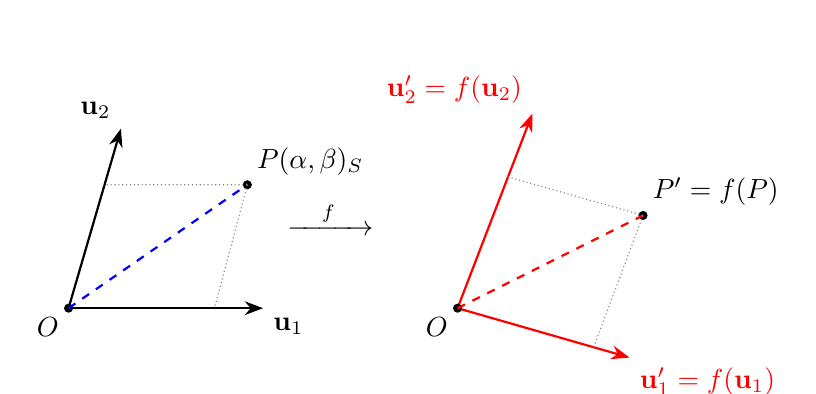
\begin{tikzpicture}[scale=0.95]
  % Domain
  \coordinate (O) at (0, 0);
  \coordinate (U1) at (1.5, 0);
  \coordinate (U2) at (0.4, 1.5);
  \draw[thick, -Stealth] (O) -- (2.6, 0) node[below right] {$\mathbf{u}_1$};
  \draw[thick, -Stealth] (O) -- (0.7, 2.4) node[above left] {$\mathbf{u}_2$};
  \filldraw (O) circle (1.5pt) node[below left] {$O$};

  \coordinate (P) at ($1.3*(U1) + 1.1*(U2)$);
  \filldraw (P) circle (1.5pt) node[above right] {$P(\alpha, \beta)_S$};
  \draw[thick, dashed, blue] (O) -- (P);
  \draw[densely dotted, gray] (P) -- ($1.3*(U1)$);
  \draw[densely dotted, gray] (P) -- ($1.1*(U2)$);

  \node at (3.5, 1.2) {$\xrightarrow{\quad f \quad}$};

  % Codomain
  \begin{scope}[shift={(5.2, 0)}]
    \coordinate (Op) at (0, 0);
    \coordinate (U1p) at (1.4, -0.4);
    \coordinate (U2p) at (0.6, 1.6);
    \draw[thick, -Stealth, red] (Op) -- (2.3, -0.66) node[below right] {$\mathbf{u}_1' = f(\mathbf{u}_1)$};
    \draw[thick, -Stealth, red] (Op) -- (1.0, 2.6) node[above left] {$\mathbf{u}_2' = f(\mathbf{u}_2)$};
    \filldraw (Op) circle (1.5pt) node[below left] {$O$};

    \coordinate (Pp) at ($1.3*(U1p) + 1.1*(U2p)$);
    \filldraw (Pp) circle (1.5pt) node[above right] {$P' = f(P)$};
    \draw[thick, dashed, red] (Op) -- (Pp);
    \draw[densely dotted, gray] (Pp) -- ($1.3*(U1p)$);
    \draw[densely dotted, gray] (Pp) -- ($1.1*(U2p)$);
  \end{scope}
\end{tikzpicture}
\caption{基底向量之映射決定全體映射}
\label{fig:b4s-1-3-5}
\end{figure}

這四個實數 $a_{11}, a_{12}, a_{21}, a_{22}$ 排成一個二列二行的數表：
\begin{equation}
[f]_S = \begin{pmatrix} a_{11} & a_{21} \\ a_{12} & a_{22} \end{pmatrix}_S \label{eq:b4s-1-3-8}
\end{equation}
稱為線性映射 $f$ 相關於座標系 $S$ 的矩陣表示，記為 $[f]_S$。特殊地，當 $S$ 取為自然座標系 $S_0$ 時，矩陣表示簡記為 $[f]$，稱為 $f$ 的自然矩陣表示：
\[ [f] = \begin{pmatrix} a_{11} & a_{21} \\ a_{12} & a_{22} \end{pmatrix} \]

\begin{example}[例 5]
試求作業 12 中 $f$ 的自然矩陣表示。
\end{example}

\begin{proof}[解]
先看自然基底經 $f$ 的寫像：
由 $f(1, 0) = (3, 2)$ 可知 $f(\mathbf{i}_1) = 3\mathbf{i}_1 + 2\mathbf{i}_2$。
由 $f(0, 1) = (-1, 1)$ 可知 $f(\mathbf{i}_2) = -1\mathbf{i}_1 + 1\mathbf{i}_2$。
故自然矩陣表示為
\[ [f] = \begin{pmatrix} 3 & -1 \\ 2 & 1 \end{pmatrix} \]
\end{proof}

\subsubsection*{作業 15}
上文中若 $A_1, A_2$ 之自然座標按序為 $(1, 0), (0, 2)$。今知 $A_1, A_2$ 經過 $f$ 的像點 $A_1', A_2'$ 之自然座標按序為 $(1, 2), (-1, 1)$。問 $P = (1.5, 0.5)$ 之像點 $P'$ 自然座標為何？又若表為 \eqref{eq:b4s-1-3-7} 式，則四實數 $a_{11}, a_{12}, a_{21}, a_{22}$ 應各為若干？

\subsubsection*{作業 16}
作業 12 中取 $\vec{OA}_1 = \mathbf{u}_1, \vec{OA}_2 = \mathbf{u}_2$，設 $S \equiv (O; \mathbf{u}_1, \mathbf{u}_2)$，問 $f$ 相關於 $S$ 之矩陣表示如何？

\subsubsection*{丁、線性映射的聯立式}

一個線性映射 $f$ 依甲段定義能表成下式：
\begin{equation}
\begin{cases}
y_1 = a_{11}x_1 + a_{21}x_2 \\
y_2 = a_{12}x_1 + a_{22}x_2
\end{cases} \label{eq:b4s-1-3-9}
\end{equation}
其中 $(y_1, y_2), (x_1, x_2)$ 皆以自然座標表之。

但這樣的型式不只採取自然座標系 $S_0$ 時才成立。實際上對任一線性映射 $f: \mathbb{R}^2 \to \mathbb{R}^2$ 及任一座標系 $S \equiv (O; \mathbf{u}_1, \mathbf{u}_2)$，$f$ 都可以這樣來表示，這是本段要說明的。

\begin{figure}[H]
\centering
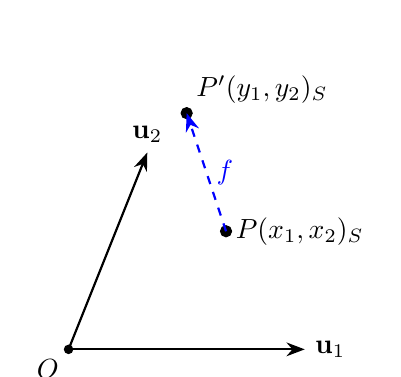
\begin{tikzpicture}[scale=1.0]
  \draw[thick, -Stealth] (0, 0) -- (3, 0) node[right] {$\mathbf{u}_1$};
  \draw[thick, -Stealth] (0, 0) -- (1, 2.5) node[above] {$\mathbf{u}_2$};
  \filldraw (0, 0) circle (1.5pt) node[below left] {$O$};
  \filldraw (2, 1.5) circle (2pt) node[right] {$P(x_1, x_2)_S$};
  \filldraw (1.5, 3.0) circle (2pt) node[above right] {$P'(y_1, y_2)_S$};
  \draw[thick, dashed, blue, -Stealth] (2, 1.5) -- (1.5, 3.0) node[midway, right] {$f$};
\end{tikzpicture}
\caption{一般座標系下的線性映射}
\label{fig:b4s-1-3-6}
\end{figure}

\begin{proposition}[命題 2]
給定一線性映射 $f$，設 $S \equiv (O; \mathbf{u}_1, \mathbf{u}_2)$，$P = (x_1, x_2)_S$ 經 $f$ 的像點 $P'$ 的座標為 $(y_1, y_2)_S$，則兩座標的關係式為：
\begin{equation}
\begin{cases}
y_1 = a_{11}x_1 + a_{21}x_2 \\
y_2 = a_{12}x_1 + a_{22}x_2
\end{cases} \label{eq:b4s-1-3-11}
\end{equation}
〔此稱為 $f$ 的座標表示式〕，其中 $(a_{ij})$ 為 $f$ 根據 $S$ 的矩陣表示，亦卽
\begin{align*}
f(\mathbf{u}_1) &= a_{11}\mathbf{u}_1 + a_{12}\mathbf{u}_2 \\
f(\mathbf{u}_2) &= a_{21}\mathbf{u}_1 + a_{22}\mathbf{u}_2
\end{align*}
\end{proposition}

\begin{theorem}[定理 4]
任一滿足“線性條件”（\eqref{eq:b4s-1-3-6} 式）之 $f: \mathbb{R}^2 \to \mathbb{R}^2$ 必為一線性映射，亦卽其自然座標間的關係可表成 \eqref{eq:b4s-1-3-4} 式。
\end{theorem}

\begin{example}[例 6]
設線性映射把 $\mathbf{u}_1 = (1, 1)$ 與 $\mathbf{u}_2 = (2, -1)$ 分別映像至 $f(\mathbf{u}_1) = (1, 0), f(\mathbf{u}_2) = (0, 1)$。試求 $f$ 相關於 $S$ 的座標表示式，並求 $P = (5, -2)_S$ 及 $Q = (-2, 5)_S$ 的像點，其中 $S \equiv (O; \mathbf{u}_1, \mathbf{u}_2)$。
\end{example}

\begin{proof}[解]
先求聯立式中之 $a_{ij}$：
\begin{align*}
(1, 0) &= a_{11}(1, 1) + a_{12}(2, -1) \implies \begin{cases} a_{11} + 2a_{12} = 1 \\ a_{11} - a_{12} = 0 \end{cases} \implies a_{11} = \frac{1}{3}, \; a_{12} = \frac{1}{3} \\
(0, 1) &= a_{21}(1, 1) + a_{22}(2, -1) \implies \begin{cases} a_{21} + 2a_{22} = 0 \\ a_{21} - a_{22} = 1 \end{cases} \implies a_{21} = \frac{2}{3}, \; a_{22} = -\frac{1}{3}
\end{align*}
故 $[f]_S = \begin{pmatrix} \frac{1}{3} & \frac{2}{3} \\ \frac{1}{3} & -\frac{1}{3} \end{pmatrix}_S$。座標表示式為：
\[ \begin{cases} y_1 = \frac{1}{3}x_1 + \frac{2}{3}x_2 \\ y_2 = \frac{1}{3}x_1 - \frac{1}{3}x_2 \end{cases} \]
代入得 $P' = (\frac{1}{3}, \frac{7}{3})_S, Q' = (\frac{8}{3}, -\frac{7}{3})_S$。
\end{proof}

\begin{figure}[H]
\centering
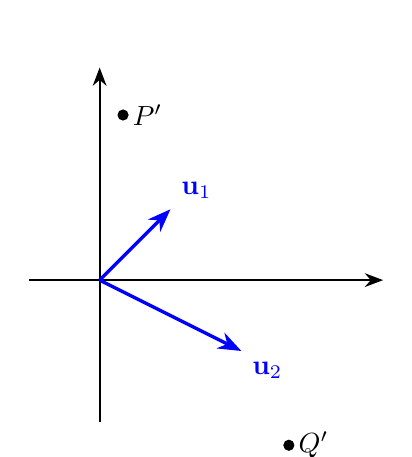
\begin{tikzpicture}[scale=0.9]
  \draw[thick, -Stealth] (-1, 0) -- (4, 0);
  \draw[thick, -Stealth] (0, -2) -- (0, 3);
  \draw[very thick, -Stealth, blue] (0, 0) -- (1, 1) node[above right] {$\mathbf{u}_1$};
  \draw[very thick, -Stealth, blue] (0, 0) -- (2, -1) node[below right] {$\mathbf{u}_2$};
  \filldraw (0.33, 2.33) circle (2pt) node[right] {$P'$};
  \filldraw (2.67, -2.33) circle (2pt) node[right] {$Q'$};
\end{tikzpicture}
\caption{例 6 之像點位置}
\label{fig:b4s-1-3-7}
\end{figure}

\begin{example}[例 7]
設 $S \equiv (O; \mathbf{u}_1, \mathbf{u}_2), \mathbf{u}_1 = (1, 1), \mathbf{u}_2 = (2, -1)$，線性映射 $f$ 相關於 $S$ 的座標表示式為 $f(x_1, x_2)_S = (3x_1 - x_2, 2x_1 + x_2)_S$。試求 $\mathbf{u}_1 = (1, 1), \mathbf{u}_2 = (2, -1)$ 經 $f$ 的映像。
\end{example}

\begin{proof}[解]
求 $\mathbf{u}_1, \mathbf{u}_2$ 經 $f$ 的映像卽在求點 $(1, 0)_S$ 及 $(0, 1)_S$ 經 $f$ 的像點的自然座標。今
\[ (1, 0)_S \mapsto (3, 2)_S, \qquad (0, 1)_S \mapsto (-1, 1)_S \]
而
\begin{align*}
(3, 2)_S &= 3(1, 1) + 2(2, -1) = (7, 1) \\
(-1, 1)_S &= -1(1, 1) + 1(2, -1) = (1, -2)
\end{align*}
故知 $f(\mathbf{u}_1) = (7, 1), f(\mathbf{u}_2) = (1, -2)$。
\end{proof}

\begin{figure}[H]
\centering
\begin{tikzpicture}[scale=0.85]
  \draw[thick, -Stealth] (-1, 0) -- (8, 0);
  \draw[thick, -Stealth] (0, -3) -- (0, 3);
  \filldraw (0, 0) circle (1.5pt) node[below left] {$O$};
  \draw[very thick, -Stealth, blue] (0, 0) -- (7, 1) node[above right] {$f(\mathbf{u}_1) = (7, 1)$};
  \draw[very thick, -Stealth, red] (0, 0) -- (1, -2) node[below right] {$f(\mathbf{u}_2) = (1, -2)$};
\end{tikzpicture}
\caption{例 7 基底向量映射}
\label{fig:b4s-1-3-8}
\end{figure}

\subsubsection*{作業 17}
\begin{enumerate}[(i)]
  \item 設 $\mathbf{u}_1 = (1, -2), \mathbf{u}_2 = (1, 0)$ 經 $f$ 的像點分別為 $(0, 1), (-1, 2)$。試求 $f$ 的座標表示式。
  \item 取 $S \equiv (O; \mathbf{u}_1, \mathbf{u}_2)$ 如 (i)，設線性映射 $f$ 相關於 $S$ 的座標表示式為 $f(x_1, x_2)_S = (2x_1 + x_2, x_1 - x_2)_S$，試求 $f(\mathbf{u}_1), f(\mathbf{u}_2)$。
\end{enumerate}

\subsubsection*{線性映射與其矩陣表示的行列式}

設 $f: \mathbb{R}^2 \to \mathbb{R}^2$ 為一線性映射，$S \equiv (O; \mathbf{e}_1, \mathbf{e}_2)$ 為 $\mathbb{R}^2$ 上任給的一個正交座標系，因
\begin{align*}
f(\mathbf{e}_1) &= a_{11}\mathbf{e}_1 + a_{12}\mathbf{e}_2 \\
f(\mathbf{e}_2) &= a_{21}\mathbf{e}_1 + a_{22}\mathbf{e}_2
\end{align*}
得其根據 $S$ 的矩陣表示為 $[f]_S = \begin{pmatrix} a_{11} & a_{21} \\ a_{12} & a_{22} \end{pmatrix}_S$。

\begin{theorem}[定理 5]
對於 $\mathbb{R}^2$ 上任意給定的正交座標系 $S$，線性映射 $f$ 為對射（或 $1-1$ 映成）的充要條件為 $\det[f]_S \neq 0$。
\end{theorem}

\begin{proof}[證明]
第三冊提過 $\left|\det \begin{pmatrix} a_{11} & a_{21} \\ a_{12} & a_{22} \end{pmatrix}\right| = |f(\mathbf{e}_1) \times f(\mathbf{e}_2)|$ 亦卽 $f(\mathbf{e}_1)$ 與 $f(\mathbf{e}_2)$ 兩向量張成的平行四邊形面積。這面積不等於零的充要條件易見為 $O, f(\mathbf{e}_1), f(\mathbf{e}_2)$ 不共線，亦卽 $f(\mathbf{e}_1)$ 與 $f(\mathbf{e}_2)$ 為線性無關，故任何平面上的向量 $\mathbf{x}'$ 皆可唯一地表成 $\mathbf{x}' = \alpha f(\mathbf{e}_1) + \beta f(\mathbf{e}_2)$。因此若取 $\mathbf{x} = \alpha\mathbf{e}_1 + \beta\mathbf{e}_2$，則 $\mathbf{x}' = f(\mathbf{x})$，且 $\mathbf{x}$ 是唯一滿足 $\mathbf{x}' = f(\mathbf{x})$ 的向量，故得證 $f$ 為對射。
\end{proof}

\begin{figure}[H]
\centering
\begin{tikzpicture}[scale=1.0]
  \draw[thick, -Stealth] (0, 0) -- (2, 0) node[right] {$\mathbf{e}_1$};
  \draw[thick, -Stealth] (0, 0) -- (0, 2) node[left=2pt] {$\mathbf{e}_2$};
  \filldraw (0, 0) circle (1.5pt) node[below left] {$O$};

  \draw[very thick, -Stealth, blue] (0, 0) -- (2.2, 0.6) node[right] {$f(\mathbf{e}_1)$};
  \draw[very thick, -Stealth, blue] (0, 0) -- (0.5, 2.2) node[above] {$f(\mathbf{e}_2)$};
  \draw[dashed, blue] (2.2, 0.6) -- (2.7, 2.8) -- (0.5, 2.2);
  \node at (1.4, 1.4) {\small 面積 $\neq 0$};
\end{tikzpicture}
\caption{非零行列式與非退化平行四邊形}
\label{fig:b4s-1-3-9}
\end{figure}

\begin{example}[例 8]
設 $f$ 為一線性映射，其自然矩陣 $[f] = \begin{pmatrix} 3 & 2 \\ 1 & 2 \end{pmatrix}$，則 $\det[f] = 3 \times 2 - 2 \times 1 = 4 \neq 0$。現給一點 $P' = (9, -2)$，我們將找出一點 $P$ 使得 $f(P) = P'$。
\end{example}

\begin{proof}[解]
因為 $f(1, 0) = (3, 1), f(0, 1) = (2, 2)$，設 $\alpha, \beta$ 滿足 $\alpha(3, 1) + \beta(2, 2) = P'$，則
\[ \begin{cases} 3\alpha + 2\beta = 9 \\ \alpha + 2\beta = -2 \end{cases} \implies \alpha = \frac{11}{2}, \; \beta = -\frac{15}{4} \]
可令 $P = (\frac{11}{2}, -\frac{15}{4})$，由原聯立方程式的條件易知 $f(P) = P'$。
\end{proof}

\subsubsection*{作業 18}
\begin{enumerate}[(i)]
  \item $f$ 為例 8 中的線性映射，$A = (\alpha, \beta)$ 為 $\mathbb{R}^2$ 上一點，若 $f(A) = (0, 0)$，則 $A = (0, 0)$。
  \item $A, B$ 為 $\mathbb{R}^2$ 不同點，則 $f(A), f(B)$ 亦為不同點。
  \item 是否 (i), (ii) 均僅用到 $\det[f] \neq 0$ 的性質？
\end{enumerate}

\subsubsection*{習題 1-3}
\begin{enumerate}
  \item 已知平面 $\mathbb{R}^2$ 上有二直線，用自然座標系 $S_0$ 時，其方程式表示如下：
  \[ L_1: x_2 = 0, \qquad L_2: x_1 - x_2 = 0 \]
  現在 $\mathbb{R}^2$ 上有一線性映射 $f$，其自然矩陣表示如下：$[f] = \begin{pmatrix} 4 & 0 \\ 0 & 1 \end{pmatrix}$。問：
  \begin{enumerate}[(i)]
    \item 直線 $L_1, L_2$ 的夾角為何？
    \item $L_1, L_2$ 經 $f$ 映射後的夾角為何？
  \end{enumerate}

  \item 用 $(x_1, x_2)$ 表自然座標，試求下列各式所定的線性映射的自然矩陣表示：
  \begin{enumerate}[a.]
    \item $f_1(1, 0) = (1, 1), f_1(0, 1) = (1, -1)$
    \item $f_2(3, 5) = (2, 1), f_2(6, 1) = (5, 7)$
    \item $f_3(1, 2) = (2, 3), f_3(3, 4) = (4, 9)$
  \end{enumerate}

  \item 仿直線的參數向量表示（設 $A, B$ 在 $L$ 上，$\mathbf{a} = \vec{OA}, \mathbf{b} = \vec{OB}$，則 $P \in L \iff \vec{OP} = \alpha\mathbf{a} + \beta\mathbf{b}$，其中 $\alpha + \beta = 1$），試證：
  \begin{enumerate}[(i)]
    \item 直線在線性映射下的像仍為直線或一點。
    \item 互相平行的兩直線在線性映射下的像仍互相平行，或重合為同一直線，或為兩相異點。
  \end{enumerate}

  \item 試求滿足下列條件的線性映射之自然矩陣表示：
  \begin{enumerate}[(i)]
    \item 把 $X$ 軸上的點固定不動，把 $Y$ 軸上的點依其到原點的距離縮小為一半。
    \item 把全體向量按逆時針方向轉動 $90^\circ$。
    \item 對直線 $x_1 - x_2 = 0$ 做鏡射。
  \end{enumerate}

  \item 設 $f$ 為一線性映射，試證下列各敘述等價：
  \begin{enumerate}[(i)]
    \item $\det[f] \neq 0$。
    \item $f$ 是單射（若 $\mathbf{a} \neq \mathbf{b}$ 則 $f(\mathbf{a}) \neq f(\mathbf{b})$）。
    \item 若 $f(\mathbf{a}) = \mathbf{0}$ 則 $\mathbf{a} = \mathbf{0}$。
    \item $f$ 是映成（對任意 $\mathbf{b}$ 存在 $\mathbf{a}$ 使得 $f(\mathbf{a}) = \mathbf{b}$）。
  \end{enumerate}

  \item 設 $f, g$ 為兩個線性映射，試證其複合映射 $g \circ f$ 亦為線性映射，且 $[g \circ f] = [g][f]$。

  \item 若矩陣 $A = \begin{pmatrix} a & b \\ c & d \end{pmatrix}$ 滿足 $ad - bc \neq 0$，試求其逆矩陣 $A^{-1}$，並證明其相應的映射 $f^{-1}$ 滿足 $f \circ f^{-1} = f^{-1} \circ f = \mathrm{id}$。

  \item 試求下列矩陣之行列式值與逆矩陣（若存在）：
  \begin{enumerate}[a.]
    \item $\begin{pmatrix} 1 & 2 \\ 3 & 4 \end{pmatrix}$
    \item $\begin{pmatrix} \cos\theta & -\sin\theta \\ \sin\theta & \cos\theta \end{pmatrix}$
    \item $\begin{pmatrix} 2 & 4 \\ 1 & 2 \end{pmatrix}$
  \end{enumerate}

  \item 設 $A$ 為平行四邊形，其四個頂點為 $(0, 0), (1, 2), (2, 1), (3, 3)$。在線性映射 $[f] = \begin{pmatrix} 2 & 1 \\ 1 & 3 \end{pmatrix}$ 之下，求 $A$ 的像 $f(A)$ 的面積與 $A$ 原面積的比值，並檢驗此比值是否等於 $\det[f]$。
\end{enumerate}
% =========================================================================
% § I-4 剛性運動與正交線性映射
% =========================================================================
\subsection{剛性運動與正交線性映射}
\label{sec:b4s-1-4}

\subsubsection*{甲、剛性運動}

在空間或平面中，最重要的一類變換是保持物體形狀與大小不變的運動。在日常生活中，我們把一塊剛體（如木塊、尺規）從一處移到另一處，其上任意兩點之間的距離都不會改變。

\begin{definition}[定義]
設 $f: \mathbb{R}^2 \to \mathbb{R}^2$ 為一映射，若對平面上任意兩點 $A, B$，均滿足
\begin{equation}
|f(A)f(B)| = |AB| \label{eq:b4s-1-4-1}
\end{equation}
則稱 $f$ 為平面 $\mathbb{R}^2$ 上的一個剛性運動（或稱等距映射，保長映射）。
\end{definition}

特殊地，若剛性運動 $f$ 把原點 $O$ 固定不動，卽 $f(O) = O$，則稱 $f$ 為定心剛性運動。

\begin{figure}[H]
\centering
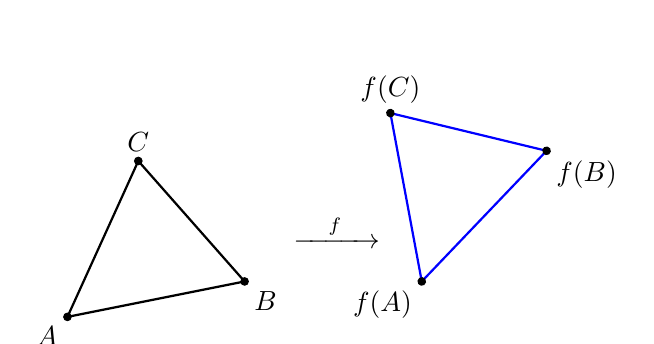
\begin{tikzpicture}[scale=0.9]
  % Original triangle
  \coordinate (A) at (0, 0);
  \coordinate (B) at (2.5, 0.5);
  \coordinate (C) at (1.0, 2.2);
  \draw[thick] (A) -- (B) -- (C) -- cycle;
  \filldraw (A) circle (1.5pt) node[below left] {$A$};
  \filldraw (B) circle (1.5pt) node[below right] {$B$};
  \filldraw (C) circle (1.5pt) node[above] {$C$};

  \node at (3.8, 1.2) {$\xrightarrow{\quad f \quad}$};

  % Rigid moved triangle
  \begin{scope}[shift={(5, 0.5)}, rotate=35]
    \coordinate (Ap) at (0, 0);
    \coordinate (Bp) at (2.5, 0.5);
    \coordinate (Cp) at (1.0, 2.2);
    \draw[thick, blue] (Ap) -- (Bp) -- (Cp) -- cycle;
    \filldraw (Ap) circle (1.5pt) node[below left] {$f(A)$};
    \filldraw (Bp) circle (1.5pt) node[below right] {$f(B)$};
    \filldraw (Cp) circle (1.5pt) node[above] {$f(C)$};
  \end{scope}
\end{tikzpicture}
\caption{剛性運動保持距離與三角形全等}
\label{fig:b4s-4-1}
\end{figure}

\begin{proposition}[命題 3]
設 $f$ 為定心剛性運動（$f(O) = O$），則對任意向量 $\mathbf{a}, \mathbf{b}$，恆有
\begin{equation}
f(\mathbf{a}) \cdot f(\mathbf{b}) = \mathbf{a} \cdot \mathbf{b} \label{eq:b4s-1-4-2}
\end{equation}
亦卽定心剛性運動保持向量的內積。
\end{proposition}

\begin{proof}[證明]
因 $f$ 保持長度，對任意向量 $\mathbf{a} = \vec{OA}$，有 $|f(\mathbf{a})| = |f(O)f(A)| = |OA| = |\mathbf{a}|$。同理 $|f(\mathbf{b})| = |\mathbf{b}|$，且 $|f(\mathbf{a}) - f(\mathbf{b})| = |f(A)f(B)| = |AB| = |\mathbf{a} - \mathbf{b}|$。

由第三冊向量內積與長度的基本公式：
\[ 2(\mathbf{a} \cdot \mathbf{b}) = |\mathbf{a}|^2 + |\mathbf{b}|^2 - |\mathbf{a} - \mathbf{b}|^2 \]
代入 $f(\mathbf{a})$ 與 $f(\mathbf{b})$：
\begin{align*}
2(f(\mathbf{a}) \cdot f(\mathbf{b})) &= |f(\mathbf{a})|^2 + |f(\mathbf{b})|^2 - |f(\mathbf{a}) - f(\mathbf{b})|^2 \\
&= |\mathbf{a}|^2 + |\mathbf{b}|^2 - |\mathbf{a} - \mathbf{b}|^2 = 2(\mathbf{a} \cdot \mathbf{b})
\end{align*}
故 $f(\mathbf{a}) \cdot f(\mathbf{b}) = \mathbf{a} \cdot \mathbf{b}$。
\end{proof}

\begin{figure}[H]
\centering
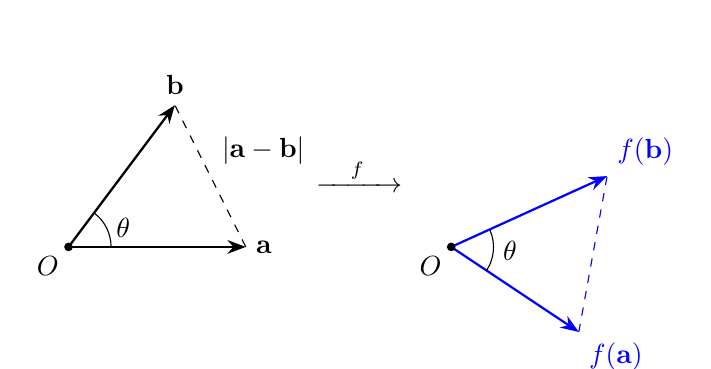
\begin{tikzpicture}[scale=0.9]
  \draw[thick, -Stealth] (0, 0) -- (2.5, 0) node[right] {$\mathbf{a}$};
  \draw[thick, -Stealth] (0, 0) -- (1.5, 2.0) node[above] {$\mathbf{b}$};
  \draw[dashed] (2.5, 0) -- (1.5, 2.0) node[midway, above right=1pt] {$|\mathbf{a}-\mathbf{b}|$};
  \draw (0.6, 0) arc (0:53:0.6) node[midway, right] {$\theta$};
  \filldraw (0, 0) circle (1.5pt) node[below left] {$O$};

  \node at (4.1, 1.0) {$\xrightarrow{\quad f \quad}$};

  \begin{scope}[shift={(5.4, 0)}]
    \draw[thick, -Stealth, blue] (0, 0) -- (1.8, -1.2) node[below right] {$f(\mathbf{a})$};
    \draw[thick, -Stealth, blue] (0, 0) -- (2.2, 1.0) node[above right] {$f(\mathbf{b})$};
    \draw[dashed, blue] (1.8, -1.2) -- (2.2, 1.0);
    \draw (0.5, -0.33) arc (-33:24:0.6) node[midway, right] {$\theta$};
    \filldraw (0, 0) circle (1.5pt) node[below left] {$O$};
  \end{scope}
\end{tikzpicture}
\caption{剛性運動保持內積與夾角}
\label{fig:b4s-4-2}
\end{figure}

\begin{proposition}[命題 4]
定心剛性運動保持向量間的夾角（保角性）。
\end{proposition}

\begin{proof}[證明]
夾角餘弦為 $\cos\theta = \dfrac{\mathbf{a} \cdot \mathbf{b}}{|\mathbf{a}| |\mathbf{b}|}$，因分子（內積）與分母（長度）在 $f$ 下皆不變，故 $\cos\theta$ 不變，卽角度不變。
\end{proof}

\begin{proposition}[命題 5]
定心剛性運動必為一線性映射。
\end{proposition}

\begin{proof}[證明]
欲證 $f(\alpha\mathbf{a} + \beta\mathbf{b}) = \alpha f(\mathbf{a}) + \beta f(\mathbf{b})$。令 $\mathbf{w} = f(\alpha\mathbf{a} + \beta\mathbf{b}) - [\alpha f(\mathbf{a}) + \beta f(\mathbf{b})]$，展開其長度平方 $|\mathbf{w}|^2 = \mathbf{w} \cdot \mathbf{w}$，利用命題 3 保持內積之性質逐項展開，可直接算得 $|\mathbf{w}|^2 = 0$，故 $\mathbf{w} = \mathbf{0}$，得證 $f$ 滿足線性條件。
\end{proof}

\subsubsection*{作業 19}
詳細寫出命題 5 證明中計算 $|\mathbf{w}|^2 = 0$ 之全部展開式。

\subsubsection*{乙、正交線性映射}

\begin{definition}[定義]
若線性映射 $f: \mathbb{R}^2 \to \mathbb{R}^2$ 保持向量之長度（亦卽對所有 $\mathbf{x} \in \mathbb{R}^2$ 均有 $|f(\mathbf{x})| = |\mathbf{x}|$），則稱 $f$ 為正交線性映射。
\end{definition}

由命題 5，定心剛性運動與正交線性映射是完全相同的概念！

設 $\{\mathbf{i}_1, \mathbf{i}_2\}$ 為自然基底，令 $\mathbf{e}_1 = f(\mathbf{i}_1), \mathbf{e}_2 = f(\mathbf{i}_2)$。因為 $f$ 保持長度與夾角，且 $\mathbf{i}_1 \perp \mathbf{i}_2, |\mathbf{i}_1| = |\mathbf{i}_2| = 1$，故 $\{\mathbf{e}_1, \mathbf{e}_2\}$ 亦為一正交基底，卽：
\[ |\mathbf{e}_1| = 1, \qquad |\mathbf{e}_2| = 1, \qquad \mathbf{e}_1 \cdot \mathbf{e}_2 = 0 \]
設 $\mathbf{e}_1 = \cos\theta \mathbf{i}_1 + \sin\theta \mathbf{i}_2$，其中 $\theta$ 為 $\mathbf{e}_1$ 的矢角（主矢角 $\theta_0 \in (-\pi, \pi]$）。因 $\mathbf{e}_2 \perp \mathbf{e}_1$ 且 $|\mathbf{e}_2| = 1$，故 $\mathbf{e}_2$ 只有兩種可能位置：
\begin{enumerate}[(i)]
  \item $\mathbf{e}_2$ 之矢角為 $\theta + \dfrac{\pi}{2}$（逆時針 $90^\circ$）。此時
  \[ \mathbf{e}_2 = \cos\left(\theta + \frac{\pi}{2}\right)\mathbf{i}_1 + \sin\left(\theta + \frac{\pi}{2}\right)\mathbf{i}_2 = -\sin\theta\mathbf{i}_1 + \cos\theta\mathbf{i}_2 \]
  \item $\mathbf{e}_2$ 之矢角為 $\theta - \dfrac{\pi}{2}$（順時針 $90^\circ$）。此時
  \[ \mathbf{e}_2 = \cos\left(\theta - \frac{\pi}{2}\right)\mathbf{i}_1 + \sin\left(\theta - \frac{\pi}{2}\right)\mathbf{i}_2 = \sin\theta\mathbf{i}_1 - \cos\theta\mathbf{i}_2 \]
\end{enumerate}

\begin{figure}[H]
\centering
\begin{tikzpicture}[scale=1.1]
  \draw[thick, -Stealth] (-1.5, 0) -- (2.5, 0) node[right] {$\mathbf{i}_1$};
  \draw[thick, -Stealth] (0, -1.5) -- (0, 2.5) node[above] {$\mathbf{i}_2$};
  \draw[gray, dashed] (0, 0) circle (1.5);
  \filldraw (0, 0) circle (1.5pt) node[below left] {$O$};

  % e1
  \draw[very thick, -Stealth, blue] (0, 0) -- (1.3, 0.75) node[above right] {$\mathbf{e}_1$};
  \draw (0.4, 0) arc (0:30:0.4) node[midway, right] {$\theta$};

  % e2 case 1: +90
  \draw[very thick, -Stealth, green!60!black] (0, 0) -- (-0.75, 1.3) node[above left] {$\mathbf{e}_2 = \vec{OE}_2$ (旋轉)};

  % e2 case 2: -90
  \draw[very thick, -Stealth, red] (0, 0) -- (0.75, -1.3) node[below right] {$\mathbf{e}_2' = \vec{OE}_2'$ (鏡射)};
\end{tikzpicture}
\caption{正交基底的兩種方向}
\label{fig:b4s-4-3}
\end{figure}

故正交線性映射的自然矩陣表示必為下列兩類之一：
\begin{equation}
\text{第一類：} \quad [f] = \begin{pmatrix} \cos\theta & -\sin\theta \\ \sin\theta & \cos\theta \end{pmatrix} \label{eq:b4s-1-4-rot-mat}
\end{equation}
\begin{equation}
\text{第二類：} \quad [f] = \begin{pmatrix} \cos\theta & \sin\theta \\ \sin\theta & -\cos\theta \end{pmatrix} \label{eq:b4s-1-4-ref-mat}
\end{equation}

\begin{example}[例 9]
設 $f$ 為一正交線性映射，其將 $\mathbf{i}_1$ 映射為 $\frac{1}{2}\mathbf{i}_1 + \frac{\sqrt{3}}{2}\mathbf{i}_2$，試求 $f$ 的可能自然矩陣表示。
\end{example}

\begin{proof}[解]
由 $\cos\theta = \frac{1}{2}, \sin\theta = \frac{\sqrt{3}}{2}$，知 $\theta = 60^\circ$。
若為第一類，$[f] = \begin{pmatrix} \frac{1}{2} & -\frac{\sqrt{3}}{2} \\ \frac{\sqrt{3}}{2} & \frac{1}{2} \end{pmatrix}$（旋轉 $60^\circ$）。
若為第二類，$[f] = \begin{pmatrix} \frac{1}{2} & \frac{\sqrt{3}}{2} \\ \frac{\sqrt{3}}{2} & -\frac{1}{2} \end{pmatrix}$（鏡射）。
\end{proof}

\subsubsection*{丙、旋轉與鏡射}

\begin{proposition}[命題 6]
當 $f: \mathbb{R}^2 \to \mathbb{R}^2$ 之自然矩陣表示為第一類 \eqref{eq:b4s-1-4-rot-mat} 時，$f$ 是平面本身以原點 $O$ 為中心、轉角為 $\theta$ 的旋轉變換。此時 $\det[f] = \cos^2\theta + \sin^2\theta = 1$。
\end{proposition}

\begin{figure}[H]
\centering
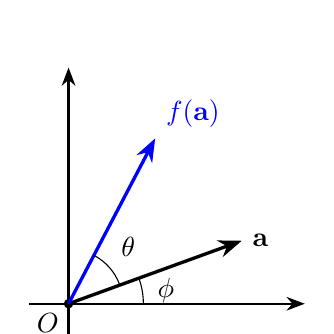
\begin{tikzpicture}[scale=1.0]
  \draw[thick, -Stealth] (-0.5, 0) -- (3, 0);
  \draw[thick, -Stealth] (0, -0.5) -- (0, 3);
  \filldraw (0, 0) circle (1.5pt) node[below left] {$O$};

  \draw[very thick, -Stealth] (0, 0) -- (2.2, 0.8) node[right] {$\mathbf{a}$};
  \draw[very thick, -Stealth, blue] (0, 0) -- (1.1, 2.1) node[above right] {$f(\mathbf{a})$};
  \draw (0.95, 0) arc (0:20:0.95) node[midway, right=2pt] {$\phi$};
  \draw (0.65, 0.24) arc (20:62:0.69) node[midway, above right=1pt] {$\theta$};
\end{tikzpicture}
\caption{旋轉變換示意圖}
\label{fig:b4s-4-4}
\end{figure}

\begin{proposition}[命題 7]
對 $f: \mathbb{R}^2 \to \mathbb{R}^2$，$f$ 為鏡射的充要條件為：存在一正交基底 $\{\mathbf{e}_1, \mathbf{e}_2\}$ 使得任意向量 $\mathbf{a} = \alpha\mathbf{e}_1 + \beta\mathbf{e}_2$，均有
\[ f(\mathbf{a}) = \alpha\mathbf{e}_1 - \beta\mathbf{e}_2 \]
此時稱 $\mathbf{e}_1$ 所在直線 $L$ 為鏡射軸。
\end{proposition}

\begin{figure}[H]
\centering
\begin{tikzpicture}[scale=1.0]
  % Mirror line L
  \draw[thick, dashed] (-1, -0.5) -- (3.5, 1.75) node[right] {$L$ (鏡射軸)};
  \draw[very thick, -Stealth, blue] (0, 0) -- (2, 1) node[above left] {$\mathbf{e}_1$};
  \draw[very thick, -Stealth, blue] (0, 0) -- (-1, 2) node[above left] {$\mathbf{e}_2$};
  \filldraw (0, 0) circle (1.5pt) node[below right=2pt] {$O$};

  % Vector a and reflection
  \coordinate (A) at (1.5, 2.5);
  \coordinate (Ap) at (2.5, 0.5);
  \filldraw (A) circle (1.5pt) node[above] {$A (\mathbf{a})$};
  \filldraw (Ap) circle (1.5pt) node[below] {$A' (f(\mathbf{a}))$};
  \draw[thick] (A) -- (Ap);
  \draw[very thick, -Stealth] (0, 0) -- (A);
  \draw[very thick, -Stealth, red] (0, 0) -- (Ap);
\end{tikzpicture}
\caption{鏡射變換幾何圖}
\label{fig:b4s-4-5}
\end{figure}

\begin{proposition}[命題 8]
當 $f: \mathbb{R}^2 \to \mathbb{R}^2$ 之自然矩陣表示為第二類 \eqref{eq:b4s-1-4-ref-mat} 時，$f$ 是平面中的一個鏡射，而其鏡射軸的傾斜角為 $\dfrac{\theta_0}{2}$，其中 $\theta_0$ 為 $\theta$ 的主矢角。此時 $\det[f] = -\cos^2\theta - \sin^2\theta = -1$。
\end{proposition}

\begin{proposition}[命題 9]
當 $f$ 之自然矩陣表示為第二類時，若取新座標系 $S \equiv (O; \mathbf{e}_1, \mathbf{e}_2)$，其中 $\mathbf{e}_1$ 為鏡射軸，則 $f$ 相關於 $S$ 的矩陣表示為
\[ [f]_S = \begin{pmatrix} 1 & 0 \\ 0 & -1 \end{pmatrix}_S \]
\end{proposition}

\begin{example}[論例 3]
設 $f$ 為轉角 $45^\circ$ 的旋轉，$g$ 為縱軸（$Y$ 軸）的鏡射，則 $g \circ f$ 亦為一鏡射。
\end{example}

\begin{proof}[證明]
因 $[f] = \begin{pmatrix} \cos 45^\circ & -\sin 45^\circ \\ \sin 45^\circ & \cos 45^\circ \end{pmatrix} = \begin{pmatrix} \frac{\sqrt{2}}{2} & -\frac{\sqrt{2}}{2} \\ \frac{\sqrt{2}}{2} & \frac{\sqrt{2}}{2} \end{pmatrix}$，$[g] = \begin{pmatrix} -1 & 0 \\ 0 & 1 \end{pmatrix}$，故
\[ [g \circ f] = [g][f] = \begin{pmatrix} -1 & 0 \\ 0 & 1 \end{pmatrix} \begin{pmatrix} \frac{\sqrt{2}}{2} & -\frac{\sqrt{2}}{2} \\ \frac{\sqrt{2}}{2} & \frac{\sqrt{2}}{2} \end{pmatrix} = \begin{pmatrix} -\frac{\sqrt{2}}{2} & \frac{\sqrt{2}}{2} \\ \frac{\sqrt{2}}{2} & \frac{\sqrt{2}}{2} \end{pmatrix} = \begin{pmatrix} \cos 135^\circ & \sin 135^\circ \\ \sin 135^\circ & -\cos 135^\circ \end{pmatrix} \]
此為第二類正交矩陣，故 $g \circ f$ 為一個對於矢角為 $\frac{135^\circ}{2} = 67.5^\circ$ 直線的鏡射。
\end{proof}

\subsubsection*{作業 20}
若 $f, g$ 為論例 3 中相同的剛性運動，$h$ 表對 $X$ 軸的鏡射：
\begin{enumerate}[(i)]
  \item 試證：$h \circ f$ 仍為一鏡射。
  \item $g \circ h$ 為一旋轉。
  \item 若 $A = (1, 0), B = (2, 1)$，而 $A' = f(A), B' = f(B)$，試證兩者張成平行四邊形面積相等，卽 $\det\begin{pmatrix} a_{11} & a_{21} \\ a_{12} & a_{22} \end{pmatrix} = \det\begin{pmatrix} 1 & 2 \\ 0 & 1 \end{pmatrix} = 1$。
\end{enumerate}

\subsubsection*{丁、總結}

\begin{theorem}[定理 7]
定心剛性運動（卽正交線性映射）不外是平面本身的旋轉或鏡射。若其自然矩陣表示為
\begin{enumerate}[(i)]
  \item $\begin{pmatrix} \cos\theta & -\sin\theta \\ \sin\theta & \cos\theta \end{pmatrix}$，則此映射便是平面本身以原點為心，轉角 $\theta$ 的一個旋轉（$\det = 1$）。
  \item $\begin{pmatrix} \cos\theta & \sin\theta \\ \sin\theta & -\cos\theta \end{pmatrix}$，則此映射便是平面中的一個鏡射，其鏡射軸的矢角為 $\dfrac{\theta}{2}$（$\det = -1$）。
\end{enumerate}
\end{theorem}

\begin{figure}[H]
\centering
\begin{tikzpicture}[scale=0.9]
  \node[draw, rounded corners, fill=blue!10, text width=6cm, align=center] (A) at (0, 2) {\textbf{定心剛性運動（保長保角）}\\$\det A = \pm 1$};
  \node[draw, rounded corners, fill=green!10, text width=4.5cm, align=center] (B) at (-3.5, -0.5) {\textbf{旋轉（Rotation）}\\$\det A = 1$\\保持平面定向（右手系）};
  \node[draw, rounded corners, fill=red!10, text width=4.5cm, align=center] (C) at (3.5, -0.5) {\textbf{鏡射（Reflection）}\\$\det A = -1$\\反轉平面定向（左手系）};
  \draw[thick, -Stealth] (A) -- (B);
  \draw[thick, -Stealth] (A) -- (C);
\end{tikzpicture}
\caption{定心剛性運動之分類體系}
\label{fig:b4s-4-6}
\end{figure}

\subsubsection*{作業 21}
轉動 $(-\theta)$ 角之旋轉，其相應的自然矩陣表示為何？特殊地，當轉角為 $-\frac{\pi}{3}$ 時，其自然矩陣表示為何？

\subsubsection*{作業 22}
設 $L$ 為下列直線，求以 $L$ 為鏡射軸的鏡射的自然矩陣表示：
\begin{enumerate}[(i)]
  \item $x - y = 0$
  \item $2x + y = 0$
  \item $y = 0$
\end{enumerate}

\subsubsection*{作業 23}
證明旋轉與鏡射的複合，仍為一鏡射，求其鏡射軸。

\subsubsection*{作業 24}
固定一點 $O$，定義函數 $f_O$ 使得 $\vec{OA'} = -\vec{OA}$。
\begin{enumerate}[(i)]
  \item 試證明 $f_O$ 為一定心剛性運動，卽對 $O$ 點旋轉 $180^\circ$。
  \item 若 $f$ 為一線性映射，且對任意 $A$ 點，$A, O, f(A)$ 三點共線，則 $f$ 為 $\alpha f_O$ 或 $\alpha \mathrm{id}$。
\end{enumerate}

\subsubsection*{作業 25}
\begin{enumerate}[(i)]
  \item 試求定心剛性運動之自然矩陣行列式值 $\det[f]$。
  \item 定心剛性運動為一旋轉的充要條件為 $\det[f] = 1$。
  \item 定心剛性運動為一鏡射的充要條件為 $\det[f] = -1$。
\end{enumerate}

\subsubsection*{作業 26}
\begin{enumerate}[(i)]
  \item $S$ 對 $X$ 軸對稱的充要條件為「$(x, y) \in S \implies (x, -y) \in S$」。
  \item $S$ 對原點對稱的充要條件為何？
\end{enumerate}

\subsubsection*{習題 1-4}
\begin{enumerate}
  \item 
  \begin{enumerate}[(i)]
    \item 試證兩個定心剛性運動相繼作用的結果仍為一定心剛性運動。
    \item 如果 $f: \mathbb{R}^2 \to \mathbb{R}^2$ 為一定心剛性運動，試證有一個唯一的剛性運動 $g$ 使得 $g \circ f = f \circ g = \mathrm{id}$。
    \item 試證 (ii) 中的 $g$ 亦為一定心剛性運動。
  \end{enumerate}

  \item 令 $S_0 \equiv (O; \mathbf{i}_1, \mathbf{i}_2)$ 為 $\mathbb{R}^2$ 的自然座標系。試以 $S_0$ 的座標表示 $\mathbf{u} = 3\mathbf{i}_1 - 4\mathbf{i}_2$ 方向的單位向量，並求以 $\mathbf{u}$ 為鏡射軸之鏡射的自然矩陣表示。

  \item 求下列各組 $\mathbf{u}$ 與 $\mathbf{u}'$ 間的角之正弦及餘弦，並求將 $\mathbf{u}$ 映射為 $\mathbf{u}'$ 的正交線性映射（旋轉與鏡射各一）：
  \begin{enumerate}[a.]
    \item $\mathbf{u} = \frac{\sqrt{3}}{2}\mathbf{i}_1 + \frac{1}{2}\mathbf{i}_2, \mathbf{u}' = \frac{1}{2}\mathbf{i}_1 + \frac{\sqrt{3}}{2}\mathbf{i}_2$
    \item $\mathbf{u} = \mathbf{i}_1 - \sqrt{3}\mathbf{i}_2, \mathbf{u}' = -\mathbf{i}_1 + \sqrt{3}\mathbf{i}_2$
  \end{enumerate}

  \item 求證平面上的映射若保長，則亦保角（提示：利用內積 $2\mathbf{a} \cdot \mathbf{b} = |\mathbf{a} + \mathbf{b}|^2 - |\mathbf{a}|^2 - |\mathbf{b}|^2$）。

  \item 證明任一剛性運動，實際上只是一個定心剛性運動與一個平移相繼作用的結果。
\end{enumerate}
% =========================================================================
% § I-5 正交座標變換
% =========================================================================
\subsection{正交座標變換}
\label{sec:b4s-1-5}

如果平面上有兩正交座標系，已知點 $P$ 相關於其中一個座標系的座標，欲求 $P$ 對另一座標系的座標。當然這樣的問題只是第 2 節所申論的一般座標變換之特殊情形。但我們已仔細討論並分類過正交座標系本身之間的線性映射，現在就利用它來直接寫出正交座標變換的形式：

我們先考慮同原點的正交座標變換：

我們不妨把兩正交座標系，取其一為自然座標系 $S_0 \equiv (O; \mathbf{i}_1, \mathbf{i}_2)$，另一正交座標系則記為 $S \equiv (O; \mathbf{e}_1, \mathbf{e}_2)$，$S_0$ 看成舊座標系，$S$ 看成新座標系。已求知（定理 7）：
\begin{equation}
\begin{cases}
\mathbf{e}_1 = \cos\theta\mathbf{i}_1 + \sin\theta\mathbf{i}_2 \\
\mathbf{e}_2 = -\sin\theta\mathbf{i}_1 + \cos\theta\mathbf{i}_2
\end{cases} \quad \text{或} \quad
\begin{cases}
\mathbf{e}_1 = \cos\theta\mathbf{i}_1 + \sin\theta\mathbf{i}_2 \\
\mathbf{e}_2 = \sin\theta\mathbf{i}_1 - \cos\theta\mathbf{i}_2
\end{cases} \label{eq:b4s-1-5-1}
\end{equation}
前者代表座標系間的旋轉，後者則代表鏡射。

其所相應的座標變換（由 § I-3 命題 2）按序應為：
\begin{equation}
\begin{cases}
x_1 = \cos\theta x_1' - \sin\theta x_2' \\
x_2 = \sin\theta x_1' + \cos\theta x_2'
\end{cases} \quad \text{或} \quad
\begin{cases}
x_1 = \cos\theta x_1' + \sin\theta x_2' \\
x_2 = \sin\theta x_1' - \cos\theta x_2'
\end{cases} \label{eq:b4s-1-5-2}
\end{equation}

\begin{figure}[H]
\centering
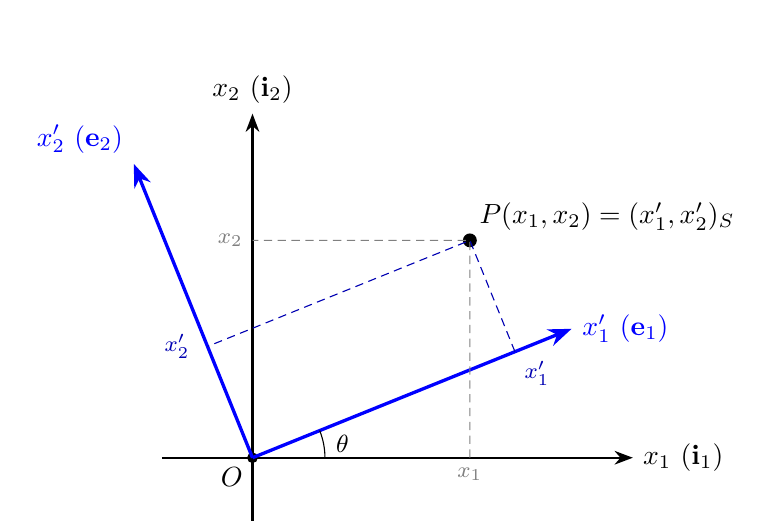
\begin{tikzpicture}[scale=1.15]
  \def\ang{22}
  \coordinate (O) at (0, 0);
  % Old axes S0
  \draw[thick, -Stealth] (-1, 0) -- (4.2, 0) node[right] {$x_1$ ($\mathbf{i}_1$)};
  \draw[thick, -Stealth] (0, -0.8) -- (0, 3.8) node[above] {$x_2$ ($\mathbf{i}_2$)};
  \filldraw (O) circle (1.5pt) node[below left] {$O$};

  % Rotated axes S
  \coordinate (E1) at (22:1);
  \coordinate (E2) at (112:1);
  \draw[very thick, -Stealth, blue] (O) -- ($3.8*(E1)$) node[right] {$x_1'$ ($\mathbf{e}_1$)};
  \draw[very thick, -Stealth, blue] (O) -- ($3.5*(E2)$) node[above left] {$x_2'$ ($\mathbf{e}_2$)};
  \draw (0.8, 0) arc (0:22:0.8) node[midway, right=1pt] {\small $\theta$};

  % Point P
  \coordinate (P) at (2.4, 2.4);
  \filldraw (P) circle (2pt) node[above right] {$P(x_1, x_2) = (x_1', x_2')_S$};

  % Projections onto old axes S0
  \draw[densely dashed, gray] (2.4, 0) node[below] {\footnotesize $x_1$} -- (P) -- (0, 2.4) node[left] {\footnotesize $x_2$};

  % Projections onto rotated axes S
  % x1' = 2.4*(cos 22 + sin 22) = 3.125
  % x2' = 2.4*(-sin 22 + cos 22) = 1.325
  \coordinate (Px1p) at ($3.125*(E1)$);
  \coordinate (Px2p) at ($1.325*(E2)$);
  \draw[densely dashed, blue!70!black] (Px1p) node[below right] {\footnotesize $x_1'$} -- (P) -- (Px2p) node[left=3pt] {\footnotesize $x_2'$};
\end{tikzpicture}
\caption{正交座標變換（轉軸）}
\label{fig:b4s-5-1}
\end{figure}

但 \eqref{eq:b4s-1-5-2} 給的是從新座標求舊座標的式子，實際上的需要常反過來。卽：已知舊座標，要求新座標，此時須分別解 \eqref{eq:b4s-1-5-2}，得：
\begin{equation}
\begin{cases}
x_1' = \cos\theta x_1 + \sin\theta x_2 \\
x_2' = -\sin\theta x_1 + \cos\theta x_2
\end{cases} \quad \text{或} \quad
\begin{cases}
x_1' = \cos\theta x_1 + \sin\theta x_2 \\
x_2' = \sin\theta x_1 - \cos\theta x_2
\end{cases} \label{eq:b4s-1-5-3}
\end{equation}
前者為旋轉，後者為鏡射的情形。

\begin{example}[例 10]
設 $S \equiv (O; \mathbf{e}_1, \mathbf{e}_2)$ 為一正交座標系，其中
\begin{align*}
\mathbf{e}_1 &= \cos 60^\circ \mathbf{i}_1 + \sin 60^\circ \mathbf{i}_2 \\
\mathbf{e}_2 &= -\sin 60^\circ \mathbf{i}_1 + \cos 60^\circ \mathbf{i}_2
\end{align*}
且 $A = (-2, 1), B = (0, 3)$，求 $A, B$ 的 $S$---座標。
\end{example}

\begin{proof}[解]
由 \eqref{eq:b4s-1-5-3} 式
\begin{align*}
A &= \left(-2\cos 60^\circ + \sin 60^\circ, \; (-2)(-\sin 60^\circ) + \cos 60^\circ\right)_S \\
&= \left(-2 \times \frac{1}{2} + \frac{\sqrt{3}}{2}, \; (-2) \times \left(-\frac{\sqrt{3}}{2}\right) + \frac{1}{2}\right)_S = \left(\frac{\sqrt{3}}{2} - 1, \; \sqrt{3} + \frac{1}{2}\right)_S \\
B &= \left(0 \times \cos 60^\circ + 3 \times \sin 60^\circ, \; 0 \times (-\sin 60^\circ) + 3 \times \cos 60^\circ\right)_S = \left(\frac{3\sqrt{3}}{2}, \; \frac{3}{2}\right)_S
\end{align*}
\end{proof}

\subsubsection*{作業 27}
設 $D$ 表座標變換式所相應的矩陣之行列式值〔卽 § I-2 \eqref{eq:b4s-1-2-5} 式提出的 $\Delta = a_{11}a_{22} - a_{12}a_{21}$〕，試驗證下列三事：
\begin{enumerate}[(i)]
  \item 正交的座標變換的 $D = \pm 1$。
  \item 當 $D = 1$ 時，卽為旋轉所對應的座標變換。
  \item 當 $D = -1$ 時，卽為鏡射所對應的座標變換。
\end{enumerate}

\subsubsection*{作業 28}
比較 \eqref{eq:b4s-1-5-1} 式和 \eqref{eq:b4s-1-5-2} 式，其間甚少差別，（代表鏡射的座標變換則完全相同），試和本章第二節中的 (4)，(5) 式相較，原因何在？

\begin{example}[例 11]
設 $S \equiv (O; \mathbf{e}_1, \mathbf{e}_2)$ 為一正交座標系，
\begin{align*}
\mathbf{e}_1 &= \cos\theta\mathbf{i}_1 - \sin\theta\mathbf{i}_2 \\
\mathbf{e}_2 &= \sin\theta\mathbf{i}_1 + \cos\theta\mathbf{i}_2
\end{align*}
若 $A = (\alpha, \beta)_S$，則 $|\vec{OA}| = \sqrt{\alpha^2 + \beta^2}$。
\end{example}

\begin{proof}[證明]
設 $A = (x_1, x_2)$ 則 $x_1 = (\cos\theta)\alpha - (\sin\theta)\beta, x_2 = (\sin\theta)\alpha + (\cos\theta)\beta$，故
\[ |\vec{OA}| = \sqrt{x_1^2 + x_2^2} = \sqrt{\alpha^2 + \beta^2} \]
\end{proof}

\subsubsection*{作業 29}
\begin{enumerate}[(i)]
  \item 在上例若 $\mathbf{e}_1 = \cos\theta\mathbf{i}_1 + \sin\theta\mathbf{i}_2, \mathbf{e}_2 = \sin\theta\mathbf{i}_1 - \cos\theta\mathbf{i}_2$，則亦有 $|\vec{OA}| = \sqrt{\alpha^2 + \beta^2}$。
  \item 若 $S \equiv (O; \mathbf{e}_1, \mathbf{e}_2)$ 為一原點不動的正交座標變換，則對任一點 $A = (\alpha, \beta)_S$ 均有 $|\vec{OA}| = \sqrt{\alpha^2 + \beta^2}$。
  \item 在 (ii) 中 $A, B$ 為任意二點，$A = (x_1, x_2)_S, B = (y_1, y_2)_S$，則 $\vec{OA} \cdot \vec{OB} = x_1 y_1 + x_2 y_2$。
\end{enumerate}

若兩正交座標系 $S_0 \equiv (O; \mathbf{i}_1, \mathbf{i}_2)$ 與 $S \equiv (O'; \mathbf{e}_1, \mathbf{e}_2)$ 的原點不一定相同，則須分兩層討論：
\begin{enumerate}[(1)]
  \item 取 $S' \equiv (O'; \mathbf{i}_1, \mathbf{i}_2)$，因與 $S$ 間的變換是旋轉或鏡射，由 \eqref{eq:b4s-1-5-2}
  \begin{equation}
  \begin{cases} x_1' = \cos\theta x_1'' - \sin\theta x_2'' \\ x_2' = \sin\theta x_1'' + \cos\theta x_2'' \end{cases} \quad \text{或} \quad
  \begin{cases} x_1' = \cos\theta x_1'' + \sin\theta x_2'' \\ x_2' = \sin\theta x_1'' - \cos\theta x_2'' \end{cases} \label{eq:b4s-1-5-4}
  \end{equation}
  \item 然後因 $S_0 \equiv (O; \mathbf{i}_1, \mathbf{i}_2)$ 與 $S' \equiv (O'; \mathbf{i}_1, \mathbf{i}_2)$ 間只差一平移，設 $\vec{OO'} = b_1\mathbf{i}_1 + b_2\mathbf{i}_2$，則
  \begin{equation}
  \begin{cases} x_1 = x_1' + b_1 \\ x_2 = x_2' + b_2 \end{cases} \label{eq:b4s-1-5-5}
  \end{equation}
\end{enumerate}
故將 \eqref{eq:b4s-1-5-4} 代入 \eqref{eq:b4s-1-5-5} 得自然座標與 $S$ 座標的關係為：
\begin{equation}
\begin{cases}
x_1 = \cos\theta x_1'' - \sin\theta x_2'' + b_1 \\
x_2 = \sin\theta x_1'' + \cos\theta x_2'' + b_2
\end{cases} \quad \text{或} \quad
\begin{cases}
x_1 = \cos\theta x_1'' + \sin\theta x_2'' + b_1 \\
x_2 = \sin\theta x_1'' - \cos\theta x_2'' + b_2
\end{cases} \label{eq:b4s-1-5-6}
\end{equation}

總結一下得：

\begin{theorem}[定理 8]
對平面上兩正交座標系 $S_0 \equiv (O; \mathbf{i}_1, \mathbf{i}_2), S \equiv (O'; \mathbf{e}_1, \mathbf{e}_2)$ 的座標變換稱為剛性座標變換，此時兩座標系之關係為：
\begin{equation}
\begin{cases}
\mathbf{e}_1 = \cos\theta\mathbf{i}_1 + \sin\theta\mathbf{i}_2 \\
\mathbf{e}_2 = -\sin\theta\mathbf{i}_1 + \cos\theta\mathbf{i}_2
\end{cases} \quad \text{或} \quad
\begin{cases}
\mathbf{e}_1 = \cos\theta\mathbf{i}_1 + \sin\theta\mathbf{i}_2 \\
\mathbf{e}_2 = \sin\theta\mathbf{i}_1 - \cos\theta\mathbf{i}_2
\end{cases} \label{eq:b4s-1-5-thm8-7}
\end{equation}
（前者為旋轉，後者為鏡射），且 $\vec{OO'} = b_1\mathbf{i}_1 + b_2\mathbf{i}_2$。

則其變換式按序為
\begin{equation}
\begin{cases}
x_1 = \cos\theta x_1' - \sin\theta x_2' + b_1 \\
x_2 = \sin\theta x_1' + \cos\theta x_2' + b_2
\end{cases} \quad \text{或} \quad
\begin{cases}
x_1 = \cos\theta x_1' + \sin\theta x_2' + b_1 \\
x_2 = \sin\theta x_1' - \cos\theta x_2' + b_2
\end{cases} \label{eq:b4s-1-5-thm8-6}
\end{equation}
其中 $(x_1, x_2), (x_1', x_2')_S$ 分別為平面上點相關於 $S_0$ 與 $S$ 的座標。

特殊地，當 $O = O'$，此時兩種座標間的變換稱同原點剛性座標變換或正交座標變換，兩組基底間的關係仍可由 \eqref{eq:b4s-1-5-thm8-7} 式給定。其座標變換式按序為
\[ \begin{cases} x_1 = \cos\theta x_1' - \sin\theta x_2' \\ x_2 = \sin\theta x_1' + \cos\theta x_2' \end{cases} \quad \text{或} \quad \begin{cases} x_1 = \cos\theta x_1' + \sin\theta x_2' \\ x_2 = \sin\theta x_1' - \cos\theta x_2' \end{cases} \]
且易解得
\[ \begin{cases} x_1' = \cos\theta x_1 + \sin\theta x_2 \\ x_2' = -\sin\theta x_1 + \cos\theta x_2 \end{cases} \quad \text{或} \quad \begin{cases} x_1' = \cos\theta x_1 + \sin\theta x_2 \\ x_2' = \sin\theta x_1 - \cos\theta x_2 \end{cases} \]
\end{theorem}

\begin{example}[例 12]
設 $S \equiv (O'; \mathbf{e}_1, \mathbf{e}_2)$ 由一剛性座標變換而得，$\vec{OO'} = \mathbf{i}_1 - \mathbf{i}_2$，$\mathbf{e}_1 = \frac{\sqrt{2}}{2}\mathbf{i}_1 + \frac{\sqrt{2}}{2}\mathbf{i}_2, \mathbf{e}_2 = \frac{\sqrt{2}}{2}\mathbf{i}_1 - \frac{\sqrt{2}}{2}\mathbf{i}_2$。已知 $A = (3, 5), B = (-2, 0)$，求 $A$ 及 $B$ 的 $S$ 座標。
\end{example}

\begin{proof}[解]
由係數比較得知 $S$ 為鏡射的情形。先計算 $A$ 點，$x_1 = 3, x_2 = 5$，代入公式解得 $x_1' = 4\sqrt{2}, x_2' = -2\sqrt{2}$，故 $A = (4\sqrt{2}, -2\sqrt{2})_S$。

同理計算點 $B$：$x_1 = -2, x_2 = 0$，得 $B = (-2\sqrt{2}, -\sqrt{2})_S$。
\end{proof}

\subsubsection*{作業 30}
設 $S$ 為上例中的座標系：
\begin{enumerate}[(i)]
  \item $A, B, C$ 之自然座標分別為 $(5, 1), (0, 3), (-2, -2)$ 求其 $S$---座標。
  \item 若 $A, B, C$ 之 $S$---座標為 $(0, 2)_S, (1, 1)_S, (-1, 3)_S$，求其自然座標。
\end{enumerate}

\subsubsection*{習題 1-5}
\begin{enumerate}
  \item 一個圓形木板半徑為 $1$ 公尺在平面上沿一直線順時鐘方向滾動，在原點取一自然座標系 $S_0 \equiv (O; \mathbf{i}_1, \mathbf{i}_2)$。另於木板上在圓心 $O'$ 上取一正交座標系 $S \equiv (O'; \mathbf{i}_1', \mathbf{i}_2')$ 固定于木板上，設木板轉動之角速度為每秒鐘一弧度。
  \begin{enumerate}[(i)]
    \item 問在轉動開始後在第 $6$ 秒鐘時，$S$ 與 $S_0$ 間的關係如何？
    \item 在起始時，木板上的點 $P$ 為 $(\frac{1}{2}, \frac{1}{2})_S$，到轉動開始後第 $10$ 秒時，點 $P$ 相關于 $S_0$ 的座標如何？
  \end{enumerate}

  \item 上題中如該木板的圓心固定在點 $O$ 順時鐘方向轉動，則答案如何？
\end{enumerate}

\vspace{1.5em}
\noindent\textbf{〔章末附註〕}\phantomsection\label{note:b4s-ch1-p57-appendix-note}

一般說來，一個映射（或稱函數）就是將一個集合 $S$ 中的元素（照）射到另一集合 $T$ 中的元素的函數。$S$ 仍稱為定義域；$T$ 為值域，寫成 $f: S \to T$。若 $s \in S$，稱 $f(s) \in T$ 為 $s$（經映射 $f$）的像點。而若 $A \subset S$，稱 $f(A)$ 為集合 $A$（經映射 $f$）的映像（Image）（或像集），記作
\[ f(A) = \{f(x) \mid x \in A\} \]

對於 $S$ 集合中不同的元素 $s_1, s_2$，若它在 $T$ 中的像點 $f(s_1)$ 與 $f(s_2)$ 也不相同，卽
\[ s_1, s_2 \in S, \; s_1 \neq s_2 \implies f(s_1) \neq f(s_2) \]
我們就說：$f$ 是嵌射的（injective）映射，或 $f$ 是嵌射（injection）（又稱單射，或一一映至）。

若對於 $T$ 中任意 $t$，存在至少一個 $s \in S$，使得 $f(s) = t$，我們就說：$f$ 是 $S$ 到 $T$ 的蓋射（surjection），或 $f$ 為蓋射的（surjective）映射（又稱全射）。

如果 $f$ 是蓋射的，又是嵌射的，就叫對射的（bijective），或 $f$ 稱為一個對射（bijection），（亦卽一一映成）。

（若 $f$ 不是蓋射的，對 $t \in T$，不必存在 $s \in S$，使得 $f(s) = t$）但是若對 $t \in T$，存在 $s \in S$ 使得 $f(s) = t$，則任意如此 $s$，均稱為 $t$ 的一個像原，我們用 $s \in f^{-1}(t)$ 表示，卽若 $B \subset T$，$S$ 的子集 $f^{-1}(B) = \{s \mid f(s) \in B\}$ 稱為 $B$ 的像原（Preimage）。

給定兩映射 $f: S \to T$ 及 $g: T \to V$，則由 $S$ 到 $V$ 的映射，使得任意 $S$ 中的元素 $s$ 的像點為：
\[ h(s) = g(f(s)) \]
稱為 $f$ 與 $g$ 的合成或複合映射，記為 $h = g \circ f$。
 % 第一章 座標變換與線性映射
% =========================================================================
% 《高中數學實驗教材》第四冊（社會組）
% 第二章 二次幾何 第一部分：錐線的演變
% =========================================================================

\section{二次幾何\texorpdfstring{\quad }{ }第一部分：錐線的演變}
\label{sec:b4s-ch2}

\begin{center}
\begin{minipage}{0.75\textwidth}
\begin{itemize}[leftmargin=2em, itemsep=0.3em]
  \item[§ II-1] \textbf{引論}
  \begin{itemize}[leftmargin=2em, itemsep=0.2em]
    \item[甲、] 拋物線
    \item[乙、] 天體運動的軌跡：二次曲線
  \end{itemize}
  \item[§ II-2] \textbf{一個關於球的切線長度的事實}
  \item[§ II-3] \textbf{圓錐曲線}
  \item[§ II-4] \textbf{焦半徑與離心率的觀點}
  \item[$\ddagger$ § II-5] \textbf{準線觀點}
\end{itemize}
\end{minipage}
\end{center}

\begin{center}
$* \qquad * \qquad * \qquad * \qquad *$
\end{center}

本冊有三個章節討論二次幾何。所謂二次幾何，在代數上指的是二元二次方程式及其所相應的多項式；在幾何上則相應於圓，橢圓，拋物線，雙曲線等曲線。本章的重點是要從圓錐與平面的截痕出發，以純幾何的方式來觀察這四種曲線如何隨著截平面的變動而互相演變，並導出它們的幾何特徵性質（焦半徑性質與準線性質）。

% =========================================================================
% § II-1 引論
% =========================================================================
\subsection{引論}
\label{sec:b4s-2-1}

\subsubsection*{甲、拋物線}

在初中我們已經學過二次函數
\begin{equation}
y = ax^2 + bx + c \quad (a \neq 0) \label{eq:b4s-2-1-1}
\end{equation}
的圖形是一條拋物線。

在物理上，拋物線有非常廣泛的應用。例如地表附近的拋體運動，如果不計空氣阻力，質點的運動軌跡就是一條拋物線（圖 \ref{fig:b4s-2-1-1}）。

\begin{figure}[H]
\centering
\begin{tikzpicture}[scale=0.9]
  \draw[thick, -Stealth] (-0.5, 0) -- (6, 0) node[right] {$x$};
  \draw[thick, -Stealth] (0, -0.5) -- (0, 3.5) node[above] {$y$};
  \filldraw (0, 0) circle (1.5pt) node[below left] {$O$};

  % Parabola projectile
  \draw[very thick, blue, domain=0:5, samples=50] plot (\x, {-0.4*(\x)*(\x - 5)});
  \draw[thick, -Stealth, red] (0, 0) -- (1.5, 2.0) node[above] {$\mathbf{v}_0$};
  \node at (2.5, 2.8) {\small 拋體運動軌跡};
\end{tikzpicture}
\caption{拋體運動之拋物線軌跡}
\label{fig:b4s-2-1-1}
\end{figure}

又如光學上，為了探照燈或汽車前燈能將光線匯聚成一束平行光，又能射達遠處，我們可利用拋物面鏡，而將燈心放在焦點 $F$ 處（圖 \ref{fig:b4s-2-1-2}）。這樣經鏡面反射的光線將平行射出，不致有漫射性的浪費，又可及於遠處。

\begin{figure}[H]
\centering
\begin{tikzpicture}[scale=0.95]
  % Parabolic mirror
  \draw[very thick, blue, domain=-2.6:2.6, samples=60] plot ({0.4*\x*\x}, \x);
  % Mirror backing hatching
  \foreach \y in {-2.4, -2.0, -1.6, -1.2, -0.8, -0.4, 0, 0.4, 0.8, 1.2, 1.6, 2.0, 2.4} {
    \draw[gray!60, thin] ({0.4*\y*\y}, \y) -- ++(-0.25, -0.15);
  }

  \coordinate (F) at (0.625, 0);

  % Light rays with arrows
  \draw[thick, -Stealth, orange!90!black] (F) -- (1.6, 2.0);
  \draw[thick, -Stealth, orange!90!black] (1.6, 2.0) -- (5.0, 2.0);

  \draw[thick, -Stealth, orange!90!black] (F) -- (0.4, 1.0);
  \draw[thick, -Stealth, orange!90!black] (0.4, 1.0) -- (5.0, 1.0);

  \draw[thick, -Stealth, orange!90!black] (F) -- (0.4, -1.0);
  \draw[thick, -Stealth, orange!90!black] (0.4, -1.0) -- (5.0, -1.0);

  \draw[thick, -Stealth, orange!90!black] (F) -- (1.6, -2.0);
  \draw[thick, -Stealth, orange!90!black] (1.6, -2.0) -- (5.0, -2.0);

  % Axis
  \draw[dashed, gray!70] (0, 0) -- (5.2, 0) node[right] {\small 對稱軸};

  % Draw focus marker and label on top of rays
  \filldraw[red!80!black] (F) circle (2pt);
  \node[red!80!black, right=8pt, fill=white, inner sep=1.5pt] at (F) {$F$ (焦點)};
\end{tikzpicture}
\caption{拋物面鏡之光學性質}
\label{fig:b4s-2-1-2}
\end{figure}

在這一光學的應用中我們所採用的只是拋物線這種形狀本身，並不計較圖 \ref{fig:b4s-2-1-1} 中它的位置。因此為了簡化，我們常將這拋物線的頂點平移到座標系的原點 $O$ 使呈右圖 \ref{fig:b4s-2-1-3} 之形狀。此時 \eqref{eq:b4s-2-1-1} 式因含 $(0, 0)$ 點，以 $x = 0$ 及 $y = 0$ 代入得 $c = 0$。又圖形對稱〔註〕於 $Y$ 軸，故 $b = 0$（見作業 1）。因此，\eqref{eq:b4s-2-1-1} 式變成
\begin{equation}
y = ax^2 \label{eq:b4s-2-1-1p}
\end{equation}
習慣上，我們考慮拋物線向兩側開口的情形，而以
\begin{equation}
y^2 = 4kx \label{eq:b4s-2-1-1pp}
\end{equation}
表示，其中為了方便取係數為 $4k$，這 \eqref{eq:b4s-2-1-1pp} 式常稱為拋物線的標準式（詳見 § III-3）。

\begin{figure}[H]
\centering
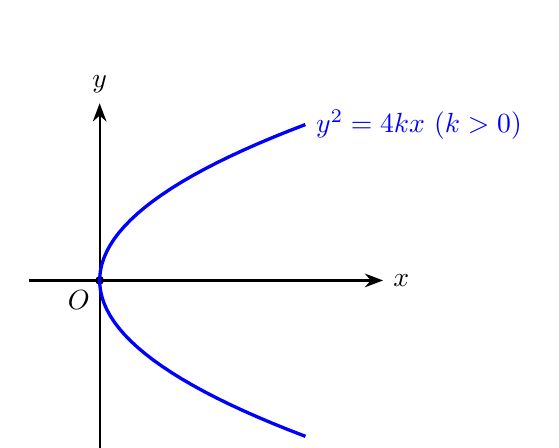
\begin{tikzpicture}[scale=0.9]
  \draw[thick, -Stealth] (-1, 0) -- (4, 0) node[right] {$x$};
  \draw[thick, -Stealth] (0, -2.5) -- (0, 2.5) node[above] {$y$};
  \filldraw (0, 0) circle (1.5pt) node[below left] {$O$};
  \draw[very thick, blue, domain=-2.2:2.2, samples=50] plot ({0.6*\x*\x}, \x) node[right] {$y^2 = 4kx$ ($k > 0$)};
\end{tikzpicture}
\caption{拋物線之標準方向}
\label{fig:b4s-2-1-3}
\end{figure}

〔註〕在座標幾何中點 $(x, y)$ 對 $Y$ 軸的對稱點為 $(-x, y)$，其對 $X$ 軸的對稱點為 $(x, -y)$，若一點在一圖形上，其對稱點亦在其上，則稱此圖形對稱。又點 $(-x, -y)$ 為 $(x, y)$ 對於原點的對稱點，而若一圖形包含一點必包含此點對原點的對稱點，則稱此圖形對稱於原點。參考第一章作業 24。

\begin{example}[論例 1]
時常我們碰到的自然現象雖非二次函數，但用二次函數來估計比用一次函數估計精確。已知電壓與電流同時為 $0$，現在我們在電壓 $x = 1.2$ 伏特時，測得電流 $y = 0.8$ 毫安培，於是由直線 $y = \frac{0.8}{1.2}x = \frac{2}{3}x$，來估計電流與電壓間的關係（一次逼近，圖 \ref{fig:b4s-2-1-4}a）。若要得到較精確的估計，可用二次函數（卽拋物線）$y = ax + bx^2$ 來估計它，這時要決定 $a, b$ 之值，我們就得做兩次實驗才夠，例如在電壓 $x = 2$ 伏特時，我們再次測得電流為 $1$ 毫安培。由
\[ \begin{cases} 0.8 = 1.2a + (1.2)^2 b \\ 1 = 2a + 2^2 b \end{cases} \]
求解 $a, b$ 得 $a = \frac{11}{12}, b = -\frac{5}{24}$，故在零點附近電流與電壓的關係可用下式估計：
\[ y = \frac{11}{12}x - \frac{5}{24}x^2 \approx 0.92x - 0.21x^2 \quad \text{（二次逼近，圖 \ref{fig:b4s-2-1-4}b）} \]
若欲得更精確的估計，我們可用多項式 $y = a_1x + a_2x^2 + \dots + a_nx^n$ 來估計它，這時我們便須做 $n$ 次測量才能定出 $a_1, a_2, \dots, a_n$。
\end{example}

\begin{figure}[H]
\centering
\begin{subfigure}[b]{0.45\textwidth}
\centering
\begin{tikzpicture}[scale=1.1]
  \draw[thick, -Stealth] (-0.3, 0) -- (3, 0) node[right] {\small 電壓 $x$};
  \draw[thick, -Stealth] (0, -0.3) -- (0, 2) node[above] {\small 電流 $y$};
  \draw[very thick, blue] (0, 0) -- (2.5, 1.67) node[right] {\small $y = \frac{2}{3}x$};
  \filldraw (1.2, 0.8) circle (1.5pt) node[below right] {\small $(1.2, 0.8)$};
\end{tikzpicture}
\caption{一次逼近}
\end{subfigure}
\hfill
\begin{subfigure}[b]{0.45\textwidth}
\centering
\begin{tikzpicture}[scale=1.1]
  \draw[thick, -Stealth] (-0.3, 0) -- (3, 0) node[right] {\small 電壓 $x$};
  \draw[thick, -Stealth] (0, -0.3) -- (0, 2) node[above] {\small 電流 $y$};
  \draw[very thick, red, domain=0:2.5, samples=50] plot (\x, {0.92*\x - 0.21*\x*\x});
  \filldraw (1.2, 0.8) circle (1.5pt) node[below right] {\small $(1.2, 0.8)$};
  \filldraw (2.0, 1.0) circle (1.5pt) node[above] {\small $(2, 1)$};
\end{tikzpicture}
\caption{二次逼近}
\end{subfigure}
\caption{電流與電壓關係之一次與二次逼近}
\label{fig:b4s-2-1-4}
\end{figure}

\subsubsection*{乙、天體運動的軌跡：二次曲線}

\eqref{eq:b4s-2-1-1} 式 $y = ax^2 + bx + c$ 中，注意只有 $x$ 的最高次項二次項。如果我們考慮一般的二元二次方程式，亦卽式中亦可帶有 $y^2, xy$ 之項如
\begin{equation}
Ax^2 + 2Bxy + Cy^2 + Dx + Ey + F = 0 \label{eq:b4s-2-1-2}
\end{equation}
（其中 $A, B, C, D, E, F$ 為實常數），則從這方程的軌跡〔稱為二次曲線〕，我們得到許多新的曲線，正是這些曲線使我們能夠妥善地描寫宇宙中一整套天體運動的軌跡及其他一些實際現象。同時透過對這些曲線的了解，我們在高中以後的課程裏將能探討二元二次函數的一些重要性質。

天體運動很多是週而復始的，這使我們很自然地想起圓。一個圓心為點 $A(a, b)$，半徑為 $r$ 的圓 $C$，其上（指圓周上）的點應是到 $A$ 的距離為定長 $r$ 的點，亦卽點 $P(x, y)$ 在 $C$ 上的充要條件是
\[ |PA| = r \iff |PA|^2 = r^2 \]
由畢氏定理知
\begin{equation}
(x - a)^2 + (y - b)^2 = r^2 \label{eq:b4s-2-1-3}
\end{equation}
與甲段的理由一樣，如只注意圓的形狀本身可移 $A$ 點至原點 $O$，而得圓的標準式
\begin{equation}
x^2 + y^2 = r^2 \label{eq:b4s-2-1-4}
\end{equation}
這是 \eqref{eq:b4s-2-1-2} 式的一種特殊形式。

\begin{figure}[H]
\centering
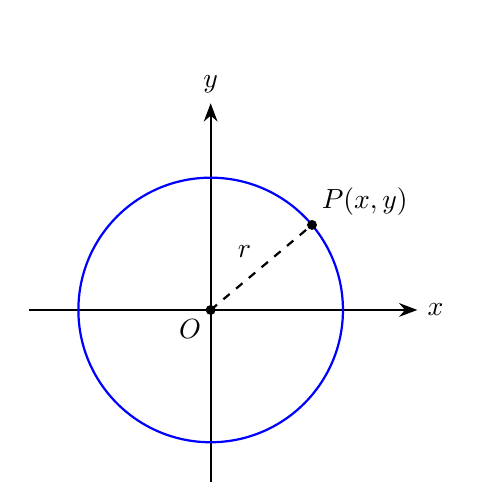
\begin{tikzpicture}[scale=1.05]
  \draw[thick, -Stealth] (-2.2, 0) -- (2.5, 0) node[right] {$x$};
  \draw[thick, -Stealth] (0, -2.2) -- (0, 2.5) node[above] {$y$};
  \draw[thick, blue] (0, 0) circle (1.6);
  \filldraw (0, 0) circle (1.5pt) node[below left] {$O$};

  \coordinate (P) at (40:1.6);
  \filldraw (P) circle (1.5pt) node[above right] {$P(x, y)$};
  \draw[thick, dashed] (0, 0) -- (P) node[midway, above left] {$r$};
\end{tikzpicture}
\caption{圓之幾何定義}
\label{fig:b4s-2-1-5}
\end{figure}

那麼圓能否描寫週而復始的天體運動？由觀測及計算的結果我們發覺：卽使只看太陽系的行星運轉，若假定太陽位置固定，行星的軌跡並不正好是圓，一般時候是呈一個壓扁了的圓的形狀，卽所謂“橢圓”。若取適當正交座標系使扁的方向為 $Y$ 軸方向（上下方），凸的方向為 $X$ 軸方向（左右方），則它的方程式相當於“分別調整 $X$ 軸與 $Y$ 軸上的距離概念”而把 \eqref{eq:b4s-2-1-4} 式變形如
\begin{equation}
\frac{x^2}{a^2} + \frac{y^2}{b^2} = 1 \quad (a, b > 0) \label{eq:b4s-2-1-5}
\end{equation}
這式子的導引將另作詳述（§ III-1）。我們稱 \eqref{eq:b4s-2-1-5} 式為橢圓的標準式。

\begin{figure}[H]
\centering
\begin{tikzpicture}[scale=1.05]
  \draw[thick, -Stealth] (-3, 0) -- (3, 0) node[right] {$x$};
  \draw[thick, -Stealth] (0, -2) -- (0, 2) node[above] {$y$};
  \draw[very thick, blue] (0, 0) ellipse (2.2 and 1.3);
  \filldraw (1.4, 0) circle (2pt) node[below=3pt, fill=white, inner sep=1pt] {$F$（太陽）};
  \filldraw (-1.4, 0) circle (2pt) node[below=3pt, fill=white, inner sep=1pt] {$F'$};
  \coordinate (P) at (-1.1, 1.12);
  \filldraw (P) circle (2pt) node[above left] {$P$（行星）};
  \draw[thick, dashed, red] (-1.4, 0) -- (P) -- (1.4, 0);
\end{tikzpicture}
\caption{克卜勒行星橢圓軌道與焦點}
\label{fig:b4s-2-1-7}
\end{figure}

圖 \ref{fig:b4s-2-1-7} 所示的行星運轉中，太陽的位置 $F$ 並不正好居中，$F$ 與其對 $Y$ 軸的鏡像點（或稱對稱點）$F'$ 合稱為橢圓的兩個焦點。這兩焦點的位置可從橢圓如下的特徵性質〔註〕求得：「橢圓上任意點 $P$ 到 $F$ 與 $F'$ 的距離和為一定長，亦卽 $|PF| + |PF'| = \text{定長}$」（見 § III-1）。

但上述週而復始的行星運行方式並不能概括所有的天體運動，比如有些彗星去而不返。當然其中一個可能原因是此星在太陽系外受到其他星體的吸引而改變初衷或消失無遺。但也有其他可能：比如它的軌道所相應的另一個焦點 $F'$ 在無窮遠處（把太陽看成固定在一個焦點 $F$ 處），這時橢圓退化成拋物線，故彗星來過一次後，便永不復返。〔上述退化現象也就是說：拋物線是橢圓頂點 $A$ 固定，而兩個焦點 $F$ 與 $F'$ 中，$F$ 固定，$F'$ 趨向無窮遠處時的極限軌跡〕見圖 \ref{fig:b4s-2-1-8}。

\begin{figure}[H]
\centering
\begin{tikzpicture}[scale=1.0]
  \draw[thick, -Stealth] (-1, 0) -- (5, 0) node[right] {$x$};
  \draw[thick, -Stealth] (0, -2.5) -- (0, 2.5) node[above] {$y$};
  \filldraw (0, 0) circle (1.5pt) node[below left] {$A$};
  \filldraw (1, 0) circle (2pt) node[below] {$F$ (太陽)};

  % Ellipses of increasing eccentricity
  \draw[thick, blue] (1.5, 0) ellipse (1.5 and 1.2);
  \draw[thick, green!60!black] (2.2, 0) ellipse (2.2 and 1.45);
  % Parabola limit
  \draw[very thick, red, domain=-2.3:2.3, samples=50] plot ({0.25*\x*\x}, \x) node[right] {拋物線 ($F' \to \infty$)};
\end{tikzpicture}
\caption{橢圓趨向拋物線之極限演變}
\label{fig:b4s-2-1-8}
\end{figure}

〔註〕數學上常用「特徵性質」這樣的字眼來代表下列特定的意義：當我們說某一性質為橢圓的特徵性質，我們不只說橢圓有這一性質而且還要求：使這性質有意義的任何數學對象必為橢圓。例如「到一角兩邊之距離等長」這一性質為分角線之特徵性質；又「到某兩點之距離等長」這一性質則為兩點連線之垂直平分線的特徵性質。

\subsubsection*{作業 1}
試用描點法繪出 $\dfrac{x^2}{4^2} + \dfrac{y^2}{3^2} = 1$ 的軌跡，並說明其對稱於原點，$X$ 軸與 $Y$ 軸（提示：點 $(\pm 4, 0)$ 及 $(0, \pm 3)$ 在其上稱為頂點，$4$ 稱為長半軸長，$3$ 稱為短半軸長）。

\subsubsection*{作業 2}
試描點繪出三橢圓
\[ \frac{x^2}{25} + \frac{y^2}{16} = 1, \qquad \frac{(x+3)^2}{64} + \frac{y^2}{25} = 1, \qquad \frac{(x+5)^2}{100} + \frac{y^2}{36} = 1 \]
與 $5y^2 = 8(-x + 5)$ 的圖形。試證後者為一端開口的曲線（卽為拋物線）而四曲線經過 $X$ 軸上一共同點。（提示：此四曲線的軸皆在 $X$ 軸，過 $X$ 軸的共同點為其公共頂點，圖類似圖 \ref{fig:b4s-2-1-8}）。

可是，力學的理論只告訴我們：一個天體相對於另一固定大天體的軌跡是一個一般二次曲線 \eqref{eq:b4s-2-1-2}，至於非週而復始的天體軌跡（如彗星）除開是拋物線外有否其他可能？

第四章二次曲線的分類將告訴我們：除開特異的情形，二次曲線在橢圓、拋物線之外尚有另一種曲線，稱為雙曲線。

比照於橢圓的標準式 \eqref{eq:b4s-2-1-5}，雙曲線的標準式為
\begin{equation}
\frac{x^2}{a^2} - \frac{y^2}{b^2} = 1 \quad (a, b > 0) \label{eq:b4s-2-1-6}
\end{equation}
（這式子的導引將在 § III-2 中詳述）。

它的軌跡由兩葉開口較拋物線為大的曲線組成（圖 \ref{fig:b4s-2-1-9}）。這兩葉曲線形狀“一樣”；換句話說它們對於對稱軸 $Y$ 軸相互成為鏡像。與橢圓情形相較，雙曲線也有一個重要的特徵性質：可取兩個所謂焦點 $F, F'$ 使雙曲線上的所有點 $P$ 到 $F$ 與 $F'$ 的距離差都為一定長，亦卽
\[ ||PF| - |PF'|| = \text{定長} \]
（詳見 § II-2）。

\begin{figure}[H]
\centering
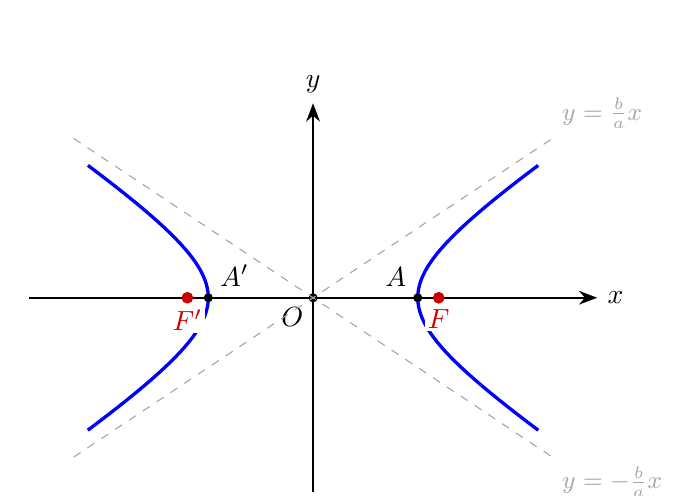
\begin{tikzpicture}[scale=0.95]
  \draw[thick, -Stealth] (-3.8, 0) -- (3.8, 0) node[right] {$x$};
  \draw[thick, -Stealth] (0, -2.6) -- (0, 2.6) node[above] {$y$};
  \filldraw (0, 0) circle (1.5pt) node[below left] {$O$};

  % Asymptotes
  \draw[dashed, gray!70] (-3.2, -2.13) -- (3.2, 2.13) node[above right] {\small $y = \frac{b}{a}x$};
  \draw[dashed, gray!70] (-3.2, 2.13) -- (3.2, -2.13) node[below right] {\small $y = -\frac{b}{a}x$};

  % Hyperbola branches (a=1.4, b=0.93)
  \draw[very thick, blue, domain=-1.4:1.4, samples=50] plot ({1.4*cosh(\x)}, {0.93*sinh(\x)});
  \draw[very thick, blue, domain=-1.4:1.4, samples=50] plot ({-1.4*cosh(\x)}, {0.93*sinh(\x)});

  % Foci c = sqrt(1.4^2 + 0.93^2) approx 1.68
  \filldraw[red!80!black] (1.68, 0) circle (2pt) node[below=3pt, fill=white, inner sep=1pt] {$F$};
  \filldraw[red!80!black] (-1.68, 0) circle (2pt) node[below=3pt, fill=white, inner sep=1pt] {$F'$};
  \filldraw (1.4, 0) circle (1.5pt) node[above left=1pt] {$A$};
  \filldraw (-1.4, 0) circle (1.5pt) node[above right=1pt] {$A'$};
\end{tikzpicture}
\caption{雙曲線與漸近線}
\label{fig:b4s-2-1-9}
\end{figure}

取雙曲線之一葉與拋物線比較，它們的一個重要差異便是前者有漸近直線或簡稱漸近線，而後者沒有（§ III-3，丙）。如圖 \ref{fig:b4s-2-1-9}，兩斜交直線卽為該雙曲線之漸近線，當點沿雙曲線向遠方伸展時，將與兩斜交直線無限接近。

其實拋物線也可看成雙曲線之極限情形。亦卽固定頂點 $A$，且固定一個焦點，讓另一焦點趨向遠處，則雙曲線逐漸退化成為拋物線，與圖 \ref{fig:b4s-2-1-8} 合在一起，可得到下圖 \ref{fig:b4s-2-1-10}：

\begin{figure}[H]
\centering
\begin{tikzpicture}[scale=1.05]
  \draw[thick, -Stealth] (-2.5, 0) -- (4.5, 0) node[right] {$x$};
  \draw[thick, -Stealth] (0, -2.5) -- (0, 2.5) node[above] {$y$};
  \filldraw (0, 0) circle (1.5pt) node[below left] {$A$};
  \filldraw (1, 0) circle (2pt) node[below=2pt, fill=white, inner sep=1pt] {$F$};

  % Ellipse sharing A and F
  \draw[thick, blue] (1.2, 0) ellipse (1.2 and 1.0);
  \node[blue] at (1.2, 1.25) {\small 橢圓};
  % Parabola sharing A and F
  \draw[very thick, green!60!black, domain=-2:2, samples=50] plot ({0.25*\x*\x}, \x);
  \node[green!60!black] at (2.4, 1.8) {\small 拋物線};
  % Hyperbola branch sharing A
  \draw[very thick, red, domain=-1.5:1.5, samples=50] plot ({0.7*(cosh(\x) - 1)}, {1.2*sinh(\x)});
  \node[red] at (3.4, 0.9) {\small 雙曲線};
\end{tikzpicture}
\caption{錐線系列演變：橢圓、拋物線、雙曲線之連續過渡}
\label{fig:b4s-2-1-10}
\end{figure}
% =========================================================================
% § II-2 一個關於球的切線長度的事實
% =========================================================================
\subsection{一個關於球的切線長度的事實}
\label{sec:b4s-2-2}

我們將用一固定圓錐與各種平面的截痕來引出所有可能的二次曲線，在這之前，先提及一個有用的事實：「球外一點到球的所有切線等長」。

取定空間的一個正交座標系 $S \equiv (O; \mathbf{e}_1, \mathbf{e}_2, \mathbf{e}_3)$，則空間中的點都可以用三個沿著一定秩序排成的實數 $x, y, z$ 來表示，亦卽，設點為 $P$，則因向量 $\vec{OP}$ 可表成
\[ \vec{OP} = x\mathbf{e}_1 + y\mathbf{e}_2 + z\mathbf{e}_3 = (x, y, z)_S \]
$P$ 與三數 $(x, y, z)_S$ 相互決定，而 $x, y, z$ 為 $\vec{OP}$ 的三個向量成分。這觀點第三冊已介紹過了。

\begin{figure}[H]
\centering
\begin{tikzpicture}[scale=0.9]
  \draw[thick, -Stealth] (0, 0) -- (3, 0) node[right] {$y$ ($\mathbf{e}_2$)};
  \draw[thick, -Stealth] (0, 0) -- (0, 3) node[above] {$z$ ($\mathbf{e}_3$)};
  \draw[thick, -Stealth] (0, 0) -- (-1.8, -1.8) node[below left] {$x$ ($\mathbf{e}_1$)};
  \filldraw (0, 0) circle (1.5pt) node[above left] {$O$};

  \coordinate (P) at (1.5, 1.8);
  \filldraw (P) circle (1.5pt) node[above right] {$P(x, y, z)$};
  \draw[very thick, -Stealth, blue] (0, 0) -- (P) node[midway, below right=2pt] {$\vec{OP}$};
\end{tikzpicture}
\caption{空間正交座標系}
\label{fig:b4s-2-2-1}
\end{figure}

球面是由所有到某一定點等距離的點組成，這定點常稱為球心，而球面上點到球心的距離稱為半徑。今空間中給定一半徑為 $r$ 的球面 $S$，若選一正交座標系 $S \equiv (O; \mathbf{e}_1, \mathbf{e}_2, \mathbf{e}_3)$ 使其基準點 $O$ 卽為球心，則空間中一點 $P = (x, y, z)_S$ 座落在這球面的充要條件為
\[ |\vec{OP}| = r \iff |\vec{OP}|^2 = r^2 \]
但根據畢氏定理 $|\vec{OP}|^2 = x^2 + y^2 + z^2$，故球面方程式為
\begin{equation}
x^2 + y^2 + z^2 = r^2 \label{eq:b4s-2-2-1}
\end{equation}

設以 $S$ 表球面，引一直線 $L$，並取自 $Q(x_0, y_0, z_0)$ 沿 $L$ 的一個單位向量 $\mathbf{u} = (\cos\alpha, \cos\beta, \cos\gamma)$。

\begin{figure}[H]
\centering
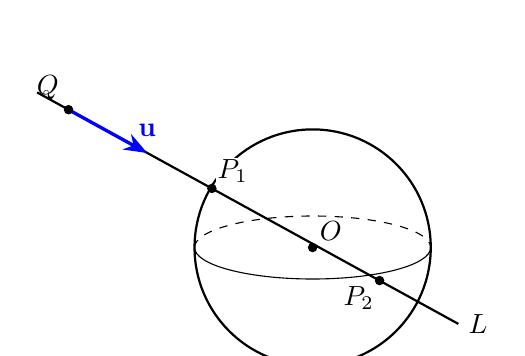
\begin{tikzpicture}[scale=1.0]
  % Sphere
  \draw[thick] (0, 0) circle (1.5);
  \draw[dashed] (-1.5, 0) arc (180:0:1.5 and 0.4);
  \draw (1.5, 0) arc (0:-180:1.5 and 0.4);
  \filldraw (0, 0) circle (1.5pt) node[above right=2pt, fill=white, inner sep=1pt] {$O$};

  % Secant Line L from Q
  \coordinate (Q) at (-3.1, 1.75);
  \coordinate (P1) at (-1.28, 0.75);
  \coordinate (P2) at (0.85, -0.42);
  \draw[thick] (-3.5, 1.97) -- (1.85, -0.97) node[right] {$L$};
  \draw[very thick, -Stealth, blue] (Q) -- (-2.1, 1.2) node[above=2pt] {$\mathbf{u}$};
  \filldraw (Q) circle (1.5pt) node[above left] {$Q$};
  \filldraw (P1) circle (1.5pt) node[above right=2pt, fill=white, inner sep=0.5pt] {$P_1$};
  \filldraw (P2) circle (1.5pt) node[below left=2pt, fill=white, inner sep=0.5pt] {$P_2$};
\end{tikzpicture}
\caption{直線與球面相交}
\label{fig:b4s-2-2-2}
\end{figure}

因此直線 $L$ 上的點 $M$ 皆可表成
\begin{align*}
\vec{OM} &= \vec{OQ} + \vec{QM} = \vec{OQ} + t\mathbf{u} \\
&= (x_0, y_0, z_0) + (t\cos\alpha, t\cos\beta, t\cos\gamma) \\
&= (x_0 + t\cos\alpha, \; y_0 + t\cos\beta, \; z_0 + t\cos\gamma)
\end{align*}
其中因 $\vec{QM} = t\mathbf{u}$，設 $L$ 上取一座標系 $S_L \equiv (Q; \mathbf{u})$，則 $t$ 可以看成 $M$ 點在 $L$ 上的 $S_L$---座標。

於是直線上點 $M$ 正好座落在球面 $S$ 上的充要條件為其座標滿足 \eqref{eq:b4s-2-2-1} 式，亦卽
\[ (x_0 + t\cos\alpha)^2 + (y_0 + t\cos\beta)^2 + (z_0 + t\cos\gamma)^2 = r^2 \]
展開，依參數 $t$ 集項得
\[ t^2(\cos^2\alpha + \cos^2\beta + \cos^2\gamma) + 2t(x_0\cos\alpha + y_0\cos\beta + z_0\cos\gamma) + (x_0^2 + y_0^2 + z_0^2 - r^2) = 0 \]
又因 $\cos^2\alpha + \cos^2\beta + \cos^2\gamma = 1$，得
\begin{equation}
t^2 + 2(x_0\cos\alpha + y_0\cos\beta + z_0\cos\gamma)t + (x_0^2 + y_0^2 + z_0^2 - r^2) = 0 \label{eq:b4s-2-2-2}
\end{equation}
這是一個 $t$ 的二次方程式，它最多有兩個實數根 $t_1$ 及 $t_2$。換句話說，直線 $L$ 最多與球面 $S$ 交於兩個點 $P_1$ 及 $P_2$。而這兩點 $P_1, P_2$ 的 $S_L$---座標分別為 $t_1, t_2$，亦卽 $\vec{QP_1} = t_1\mathbf{u}, \vec{QP_2} = t_2\mathbf{u}$。

注意因 $\mathbf{u}$ 為單位向量，$|t_1|$ 及 $|t_2|$ 正好代表 $Q$ 到 $P_1$ 與 $P_2$ 的距離，卽 $|t_1| = |QP_1|, |t_2| = |QP_2|$。

由 \eqref{eq:b4s-2-2-2} 式之根與係數的關係，當 $Q$ 在球外，$P_1$ 與 $P_2$ 落在 $Q$ 的同側，$t_1$ 與 $t_2$ 同號，故此時
\begin{equation}
|QP_1| \cdot |QP_2| = t_1 t_2 = x_0^2 + y_0^2 + z_0^2 - r^2 = |\vec{OQ}|^2 - r^2 \label{eq:b4s-2-2-3}
\end{equation}

\begin{definition}[定義]
空間中直線 $L$ 若與球面 $S$ 相交於兩點 $P_1$ 及 $P_2$，$L$ 稱為 $S$ 的割線。若只交於一點時，亦卽 $P_1$ 與 $P_2$ 重合時，$L$ 稱為 $S$ 的切線，或稱 $L$ 切於 $S$，此時 $L$ 上一點 $Q$ 到切點的距離稱為 $Q$ 到球面 $S$ 的切線長。
\end{definition}

當 $L$ 切於 $S$ 時，$P_1$ 與 $P_2$ 重合（稱切點 $P$），卽
\begin{equation}
|QP|^2 = |\vec{OQ}|^2 - r^2 \label{eq:b4s-2-2-4}
\end{equation}
更因左端 $\ge 0$，故 $|\vec{OQ}|^2 - r^2 \ge 0$，知當 $L$ 切於球面時，$Q$ 不落在球的內部。進一步由廣義畢氏定理，\eqref{eq:b4s-2-2-4} 式告訴我們 $\angle OPQ$ 成一直角，亦卽切線垂直於過切點的半徑。

歸結本節所述可得：

\begin{theorem}[定理 1（球的割線定理）]
空間中給定一點 $Q$ 及一以 $O$ 為心，以 $r$ 為半徑的球面 $S$，則過該點 $Q$ 的任一直線 $L$ 最多只能交球面於兩點 $P_1, P_2$，若 $L$ 上取一座標系 $S_L \equiv (Q; \mathbf{u})$，$P_1, P_2$ 的 $S_L$---座標分別為 $t_1, t_2$，則當 $Q$ 在球外，恆有
\[ |QP_1| \cdot |QP_2| = |\vec{OQ}|^2 - r^2 \]
\end{theorem}

\begin{theorem}[定理 1'（球的切線長定理）]
球外給定一點 $Q$ 到球的切線垂直於過切點的半徑，且所有這些切線等長，皆為定值：
\[ \sqrt{|\vec{OQ}|^2 - r^2} \]
其中 $O$ 為球心，$r$ 為球半徑。
\end{theorem}

\subsubsection*{習題 2-2}
\begin{enumerate}
  \item 求 $(4, 1, 1)$ 至球面 $(x+1)^2 + y^2 + (z-2)^2 = 16$ 的切線長。
  \item 設過點 $Q(3, 2, 1)$ 之直線 $L$ 與球面 $x^2 + y^2 + z^2 = 4$ 相交於 $P_1, P_2$ 兩點，求 $|QP_1| \cdot |QP_2|$ 之值。
  \item 求過點 $(0, 0, 0)$ 與直線 $\frac{x-1}{2} = \frac{y-2}{1} = \frac{z-3}{2}$ 上點到球面 $(x+1)^2 + y^2 + (z-2)^2 = 16$ 之交點。
  \item 試證：至二球面 $S_1, S_2$ 切線長相等的點的軌跡為一平面 $\pi$（$\pi$ 稱為二球面的根平面）。
\end{enumerate}

% =========================================================================
% § II-3 圓錐曲線
% =========================================================================
\subsection{圓錐曲線}
\label{sec:b4s-2-3}

本章我們的用意是要從圓錐與平面的截痕（將稱為圓錐曲線或簡稱錐線）得到各種二次曲線；這節我們先直觀地來看各種圓錐曲線如何隨著截平面而演變。

\begin{definition}[定義]
所謂圓錐面便是在空間中，取定一平面及其上兩條相交於一點 $K$ 的直線 $L_0$ 及 $L_1$，然後以 $L_0$ 為固定軸將平面迴轉，此時，另一直線 $L_1$ 掃出一個錐狀的曲面，這樣得到的曲面便稱為圓錐面，設以 $\Omega$ 記之，$K$ 稱為圓錐 $\Omega$ 的頂點，$L_0$ 稱為 $\Omega$ 的中心軸，迴轉中的 $L_1$ 在任一時刻的位置是一條 $\Omega$ 上的直線，稱為 $\Omega$ 的一條母線。而 $L_0$ 與 $L_1$ 的夾角 $\omega$ 則稱圓錐的頂半角（此角為一定角，不隨 $L_1$ 的迴轉而改變）。
\end{definition}

\begin{figure}[H]
\centering
\begin{tikzpicture}[scale=0.9]
  % Cone apex
  \coordinate (K) at (0, 0);
  % Upper cone
  \draw[thick] (K) -- (-2, 3);
  \draw[thick] (K) -- (2, 3);
  \draw[thick] (0, 3) ellipse (2 and 0.5);
  % Lower cone
  \draw[thick] (K) -- (-2, -3);
  \draw[thick] (K) -- (2, -3);
  \draw[thick] (0, -3) ellipse (2 and 0.5);
  % Axis L0
  \draw[dashed, very thick] (0, -3.8) -- (0, 3.8) node[above] {$L_0$ (中心軸)};
  \filldraw (K) circle (2pt) node[right] {$K$ (頂點)};
  % Angle omega
  \draw (0, 1.2) arc (90:124:1.2) node[midway, above] {$\omega$};
\end{tikzpicture}
\caption{圓錐面及其組成要素}
\label{fig:b4s-2-3-1}
\end{figure}

\begin{definition}[定義]
設 $\Omega$ 為一以 $K$ 為頂點的圓錐。一個不含 $K$ 的平面 $\pi$ 與 $\Omega$ 的截痕稱為圓錐曲線，或簡稱錐線。不妨將 $\Omega$ 固定使之正立，而中心軸 $L_0$ 鉛垂向上。當截平面 $\pi$ 交中心軸 $L_0$ 於一點 $M$ 時，取 $\pi$ 的一個單位法向量 $\mathbf{u} = \vec{MN}$ 使 $N$ 與頂點 $K$ 在 $\pi$ 的同側。取一平面 $\pi_0$ 含 $L_0$ 與 $MN$，稱法向量與中心軸的夾角 $\theta$ 為 $\pi$ 在 $\Omega$ 上的截角。當 $\pi$ 不與 $L_0$ 相交於一點時，定義截角 $\theta = \frac{\pi}{2}$。
\end{definition}

在介紹本題之前我們引入兩個直觀立體幾何的定理：

\begin{theorem}[定理 2]
設 $L_1$ 為平面 $\pi$ 的垂線，$\pi_1$ 為任意含 $L_1$ 的平面，交 $\pi$ 於直線 $L$，若自 $\pi_1$ 上一點 $P$ 引 $L$ 的垂線 $PN$（交 $L$ 於 $N$），則 $PN$ 亦為平面 $\pi$ 的垂線。
\end{theorem}

\begin{figure}[H]
\centering
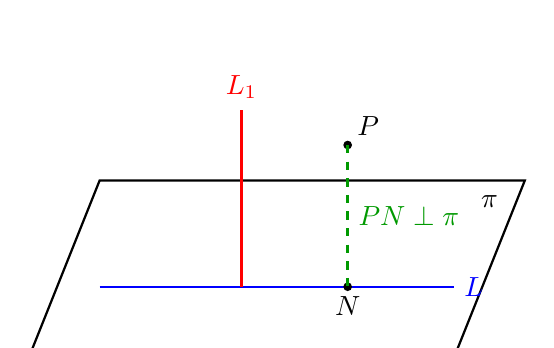
\begin{tikzpicture}[scale=0.9]
  % Plane pi
  \draw[thick] (-2, -1) -- (4, -1) -- (5, 1.5) -- (-1, 1.5) -- cycle;
  \node at (4.5, 1.2) {$\pi$};
  % Intersection line L
  \draw[thick, blue] (-1, 0) -- (4, 0) node[right] {$L$};
  % Perpendicular line L1
  \draw[very thick, red] (1, 0) -- (1, 2.5) node[above] {$L_1$};
  % Point P and PN
  \coordinate (P) at (2.5, 2);
  \coordinate (N) at (2.5, 0);
  \filldraw (P) circle (1.5pt) node[above right] {$P$};
  \filldraw (N) circle (1.5pt) node[below] {$N$};
  \draw[very thick, dashed, green!60!black] (P) -- (N) node[midway, right] {$PN \perp \pi$};
\end{tikzpicture}
\caption{定理 2 垂線性質示意圖}
\label{fig:b4s-2-3-3}
\end{figure}

\begin{theorem}[定理 3（三垂線定理）]
設 $L$ 垂直於平面 $\pi$，垂足為 $M$，$L'$ 為 $\pi$ 上一直線，若自直線 $L$ 上一點 $P$ 引 $L'$ 的垂線（在由 $P$ 與 $L'$ 所決定的平面上引這垂線），垂足為 $N$，則 $MN \perp L'$。
\end{theorem}

\begin{figure}[H]
\centering
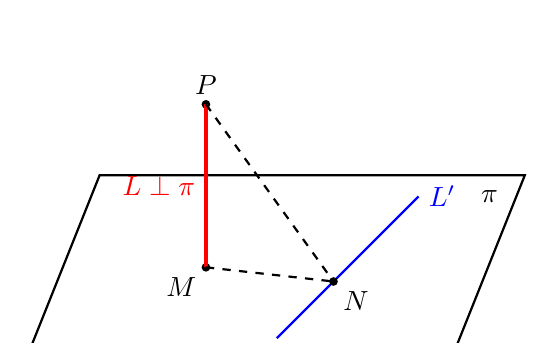
\begin{tikzpicture}[scale=0.9]
  % Plane pi
  \draw[thick] (-2, -1) -- (4, -1) -- (5, 1.5) -- (-1, 1.5) -- cycle;
  \node at (4.5, 1.2) {$\pi$};
  \coordinate (M) at (0.5, 0.2);
  \coordinate (P) at (0.5, 2.5);
  \filldraw (M) circle (1.5pt) node[below left] {$M$};
  \filldraw (P) circle (1.5pt) node[above] {$P$};
  \draw[very thick, red] (M) -- (P) node[midway, left] {$L \perp \pi$};

  % Line L' in pi
  \draw[thick, blue] (1.5, -0.8) -- (3.5, 1.2) node[right] {$L'$};
  \coordinate (N) at (2.3, 0);
  \filldraw (N) circle (1.5pt) node[below right] {$N$};

  \draw[thick, dashed] (P) -- (N);
  \draw[thick, dashed] (M) -- (N);
\end{tikzpicture}
\caption{三垂線定理示意圖}
\label{fig:b4s-2-3-4}
\end{figure}

回到我們的本題：當圓錐面 $\Omega$ 固定，相應的圓錐曲線 $\Gamma$ 隨著截平面 $\pi$ 在 $\Omega$ 上的截角 $\theta$ 的變化而從正圓，橢圓，變成拋物線，再變為雙曲線。令 $\omega' = \frac{\pi}{2} - \omega$ 為母線與中心軸垂直面之夾角（頂半角的餘角）：
\begin{enumerate}[(i)]
  \item 當 $\theta$ 在 $0$ 與 $\omega'$ 之間（$0 \le \theta < \omega'$）時，截痕為“橢圓”模樣（特殊地當 $\theta = 0$ 時，截痕 $\Gamma$ 為正圓）。
  \item 當 $\theta = \omega'$ 時，截面與一條母線平行，截痕 $\Gamma$ 為拋物線模樣。
  \item 當 $\theta > \omega'$ 時，截面與圓錐兩葉皆相交，截痕 $\Gamma$ 擴大為兩葉，呈“雙曲線”形狀。
\end{enumerate}

\begin{figure}[H]
\centering
\begin{tikzpicture}[scale=0.8]
  % Three cone sections
  \begin{scope}[shift={(0, 0)}]
    \draw (-1.5, 2) -- (0, 0) -- (1.5, 2);
    \draw (-1.5, -2) -- (0, 0) -- (1.5, -2);
    \draw[blue, thick] (0, 1.2) ellipse (0.8 and 0.3);
    \node at (0, -2.5) {\small (i) $0 \le \theta < \omega'$（橢圓/圓）};
  \end{scope}

  \begin{scope}[shift={(5.3, 0)}]
    \draw (-1.5, 2) -- (0, 0) -- (1.5, 2);
    \draw (-1.5, -2) -- (0, 0) -- (1.5, -2);
    \draw[green!60!black, thick] (-0.8, 1.8) parabola bend (0.3, 0.4) (1.2, 1.8);
    \node at (0, -2.5) {\small (ii) $\theta = \omega'$（拋物線）};
  \end{scope}

  \begin{scope}[shift={(10.6, 0)}]
    \draw (-1.5, 2) -- (0, 0) -- (1.5, 2);
    \draw (-1.5, -2) -- (0, 0) -- (1.5, -2);
    \draw[red, thick] (-0.6, 1.8) parabola bend (0.2, 0.5) (0.8, 1.8);
    \draw[red, thick] (-0.6, -1.8) parabola bend (0.2, -0.5) (0.8, -1.8);
    \node at (0, -2.5) {\small (iii) $\theta > \omega'$（雙曲線）};
  \end{scope}
\end{tikzpicture}
\caption{圓錐截痕之分類演變}
\label{fig:b4s-2-3-5}
\end{figure}

至於當截平面 $\pi$ 通過圓錐頂點 $K$ 時，在上述 (i), (ii), (iii) 的條件下，所得的截痕分別為一點、一直線或兩相交直線，稱為退化二次曲線。
% =========================================================================
% § II-4 焦半徑與離心率的觀點
% =========================================================================
\subsection{焦半徑與離心率的觀點}
\label{sec:b4s-2-4}

現在我們要利用 § II-2 的球切線長定理，來導出圓錐截痕的焦點與焦半徑性質。這個精妙的幾何構想是 1822 年由比利時數學家丹德林（Dandelin）所發現的，稱為丹德林雙球定理。

\subsubsection*{甲、負類錐線（橢圓）}

在圓錐面 $\Omega$ 內放置兩個大小適當的球 $S$ 與 $S'$，使其分別與截平面 $\pi$ 相切於 $F$ 與 $F'$ 兩點，同時又與圓錐面 $\Omega$ 沿兩個水平圓周 $C_1$ 與 $C_2$ 相切（圖 \ref{fig:b4s-2-4-1}）。這兩切點 $F$ 與 $F'$ 卽為錐線的兩個焦點。

\begin{figure}[H]
\centering
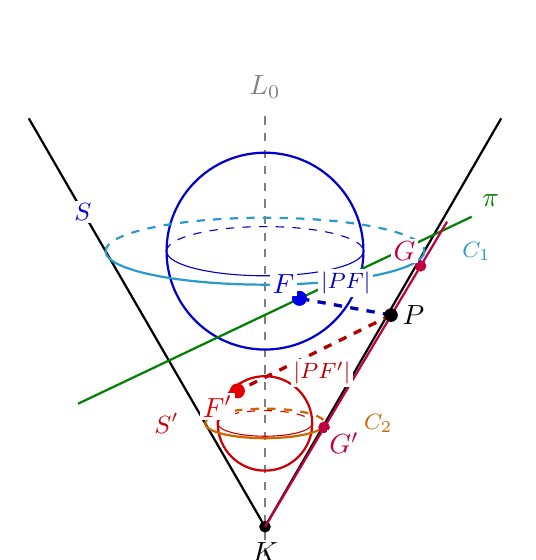
\begin{tikzpicture}[scale=1.25]
  % Cone outline
  \coordinate (K) at (0, 0);
  \draw[thick] (-2.4, 4.15) -- (K) -- (2.4, 4.15);
  \draw[dashed, gray] (0, -0.3) -- (0, 4.25) node[above] {$L_0$};
  \filldraw (K) circle (1.5pt) node[below=2pt] {$K$};

  % Sphere S (upper, larger)
  \coordinate (O1) at (0, 2.8);
  \draw[blue!80!black, thick] (O1) circle (1.0);
  \draw[blue!80!black, dashed] (-1.0, 2.8) arc (180:0:1.0 and 0.25);
  \draw[blue!80!black] (1.0, 2.8) arc (0:-180:1.0 and 0.25);
  \node[blue!80!black, fill=white, inner sep=1pt] at (-1.85, 3.2) {\small $S$};

  % Contact circle C1 where S touches the cone
  \draw[cyan!80!black, thick, dashed] (-1.62, 2.8) arc (180:0:1.62 and 0.34);
  \draw[cyan!80!black, thick] (1.62, 2.8) arc (0:-180:1.62 and 0.34);
  \node[cyan!80!black, fill=white, inner sep=1pt] at (2.15, 2.8) {\footnotesize $C_1$};

  % Sphere S' (lower, smaller)
  \coordinate (O2) at (0, 1.05);
  \draw[red!80!black, thick] (O2) circle (0.48);
  \draw[red!80!black, dashed] (-0.48, 1.05) arc (180:0:0.48 and 0.13);
  \draw[red!80!black] (0.48, 1.05) arc (0:-180:0.48 and 0.13);
  \node[red!80!black, fill=white, inner sep=1pt] at (-1.0, 1.05) {\small $S'$};

  % Contact circle C2 where S' touches the cone
  \draw[orange!80!black, thick, dashed] (-0.61, 1.05) arc (180:0:0.61 and 0.15);
  \draw[orange!80!black, thick] (0.61, 1.05) arc (0:-180:0.61 and 0.15);
  \node[orange!80!black, fill=white, inner sep=1pt] at (1.15, 1.05) {\footnotesize $C_2$};

  % Cutting plane pi
  \draw[thick, green!50!black] (-1.9, 1.25) -- (2.1, 3.15) node[above right] {$\pi$};
  \coordinate (F) at (0.35, 2.32);
  \coordinate (Fp) at (-0.28, 1.38);

  % Point P on ellipse (on generatrix from K to G)
  \coordinate (G) at (1.58, 2.65);
  \coordinate (Gp) at (0.60, 1.01);
  \coordinate (P) at (1.28, 2.15);

  % Generatrix KP cutting C1 at G and C2 at G'
  \draw[purple, thick] (K) -- (1.85, 3.10);

  % Tangents from P to F and F'
  \draw[very thick, dashed, blue!70!black] (P) -- (F);
  \draw[very thick, dashed, red!70!black] (P) -- (Fp);

  % Labels placed cleanly on top
  \filldraw[blue!90!black] (F) circle (2pt) node[above left=1pt, fill=white, inner sep=1pt] {$F$};
  \filldraw[red!90!black] (Fp) circle (2pt) node[below left=1pt, fill=white, inner sep=1pt] {$F'$};
  \filldraw (P) circle (1.8pt) node[right=3pt, fill=white, inner sep=1pt] {$P$};
  \filldraw[purple] (G) circle (1.5pt) node[above left=1pt, fill=white, inner sep=1pt] {$G$};
  \filldraw[purple] (Gp) circle (1.5pt) node[below right=1pt, fill=white, inner sep=1pt] {$G'$};

  \node[blue!70!black, fill=white, inner sep=1pt] at (0.82, 2.48) {\footnotesize $|PF|$};
  \node[red!70!black, fill=white, inner sep=1pt] at (0.58, 1.56) {\footnotesize $|PF'|$};
\end{tikzpicture}
\caption{丹德林雙球與橢圓焦半徑性質}
\label{fig:b4s-2-4-1}
\end{figure}

設 $P$ 為截痕 $\Gamma$ 上的任意點，連結母線 $KP$，交圓 $C_1$ 於 $G$，交圓 $C_2$ 於 $G'$。因為直線 $PF$ 與 $PG$ 都是自點 $P$ 引至球 $S$ 的切線，由定理 1'，
\[ |PF| = |PG| \]
同理，直線 $PF'$ 與 $PG'$ 都是自點 $P$ 引至球 $S'$ 的切線，故
\[ |PF'| = |PG'| \]
相加得
\[ |PF| + |PF'| = |PG| + |PG'| = |GG'| \]
但線段 $GG'$ 夾在兩水平切圓 $C_1$ 與 $C_2$ 之間，其長度只決定於兩切圓間沿母線的距離，與點 $P$ 的選取完全無關！因此 $|GG'|$ 為一常數，記為 $2a$。

\begin{proposition}[命題 1（負類錐線焦半徑性質）]
對於負類錐線（橢圓）$\Gamma$ 上的任意點 $P$，恆有
\begin{equation}
|PF| + |PF'| = |GG'| = 2a = \text{定長} \label{eq:b4s-2-4-1}
\end{equation}
\end{proposition}

\begin{corollary}[系理 1]
設截面交中心對稱平面於兩頂點 $A, A'$，則
\[ |AF| = |A'F'| \]
\end{corollary}

\begin{definition}[定義]
負類錐線（橢圓）的離心率定義為兩焦點距離與兩頂點距離之比：
\begin{equation}
e = \frac{|FF'|}{|AA'|} = \frac{2c}{2a} = \frac{c}{a} \label{eq:b4s-2-4-ecc}
\end{equation}
因為兩焦點 $F, F'$ 落在頂點 $A, A'$ 內部，故恆有 $0 \le e < 1$。特別地，當截面水平時，$F = F'$ 重合為圓心，此時 $e = 0$（正圓）。
\end{definition}

\subsubsection*{乙、零類錐線（拋物線）}

當截角 $\theta = \omega'$ 時，截平面與圓錐的一條母線平行，此時只能在圓錐內放入一個與截面及圓錐相切的球 $S$（另一個球跑到無窮遠處），故拋物線只有一個焦點 $F$。離心率規定為 $e = 1$。

\begin{proposition}[命題 2]
拋物線可視為橢圓當另一焦點 $F'$ 趨向無窮遠處時之極限情況。
\end{proposition}

\subsubsection*{丙、正類錐線（雙曲線）}

當截角 $\theta > \omega'$ 時，截面與圓錐的上下兩葉皆相交，截痕為雙曲線。此時丹德林雙球分別位於圓錐頂點 $K$ 的兩側：一個在頂點上葉內切於球 $S$，切點為 $F$；另一個在頂點下葉內切於球 $S'$，切點為 $F'$（圖 \ref{fig:b4s-2-4-7}）。

\begin{figure}[H]
\centering
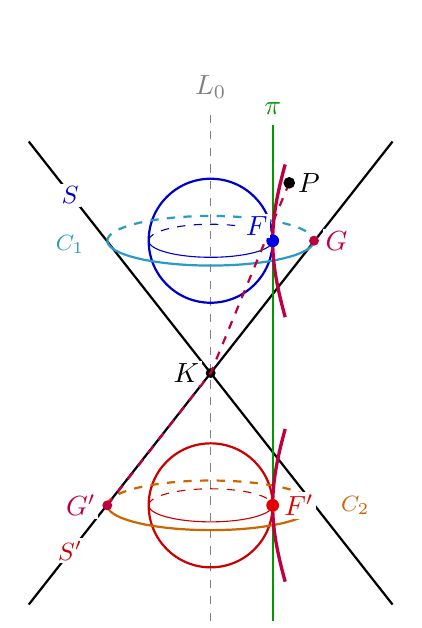
\begin{tikzpicture}[scale=1.05]
  % Double cone outline
  \coordinate (K) at (0, 0);
  \draw[thick] (-2.2, 2.8) -- (K) -- (2.2, 2.8);
  \draw[thick] (-2.2, -2.8) -- (K) -- (2.2, -2.8);
  \draw[dashed, gray] (0, -3.2) -- (0, 3.2) node[above] {$L_0$};
  \filldraw (K) circle (1.5pt) node[left=3pt, fill=white, inner sep=1pt] {$K$};

  % Sphere in upper cone S
  \coordinate (O1) at (0, 1.6);
  \draw[blue!80!black, thick] (O1) circle (0.75);
  \draw[blue!80!black, dashed] (-0.75, 1.6) arc (180:0:0.75 and 0.2);
  \draw[blue!80!black] (0.75, 1.6) arc (0:-180:0.75 and 0.2);
  \node[blue!80!black, fill=white, inner sep=1pt] at (-1.7, 2.15) {\small $S$};

  % Contact circle C1
  \draw[cyan!80!black, thick, dashed] (-1.25, 1.6) arc (180:0:1.25 and 0.3);
  \draw[cyan!80!black, thick] (1.25, 1.6) arc (0:-180:1.25 and 0.3);
  \node[cyan!80!black, fill=white, inner sep=1pt] at (-1.7, 1.55) {\footnotesize $C_1$};

  % Sphere in lower cone S'
  \coordinate (O2) at (0, -1.6);
  \draw[red!80!black, thick] (O2) circle (0.75);
  \draw[red!80!black, dashed] (-0.75, -1.6) arc (180:0:0.75 and 0.2);
  \draw[red!80!black] (0.75, -1.6) arc (0:-180:0.75 and 0.2);
  \node[red!80!black, fill=white, inner sep=1pt] at (-1.7, -2.15) {\small $S'$};

  % Contact circle C2
  \draw[orange!80!black, thick, dashed] (-1.25, -1.6) arc (180:0:1.25 and 0.3);
  \draw[orange!80!black, thick] (1.25, -1.6) arc (0:-180:1.25 and 0.3);
  \node[orange!80!black, fill=white, inner sep=1pt] at (1.75, -1.6) {\footnotesize $C_2$};

  % Cutting plane pi
  \draw[thick, green!60!black] (0.75, -3.0) -- (0.75, 3.0) node[above] {$\pi$};
  \coordinate (F) at (0.75, 1.6);
  \coordinate (Fp) at (0.75, -1.6);

  % Hyperbolic branches on plane pi
  \draw[very thick, purple, domain=-0.9:0.9, samples=40] plot ({0.75 + 0.35*(cosh(\x)-1)}, {1.6 + 0.9*sinh(\x)});
  \draw[very thick, purple, domain=-0.9:0.9, samples=40] plot ({0.75 + 0.35*(cosh(\x)-1)}, {-1.6 - 0.9*sinh(\x)});

  % Point P and generatrix KP
  \coordinate (P) at (0.95, 2.3);
  \coordinate (G) at (1.25, 1.6);
  \coordinate (Gp) at (-1.25, -1.6);
  \draw[thick, dashed, purple] (Gp) -- (K) -- (P);

  % Labels drawn on top
  \filldraw[blue!90!black] (F) circle (2pt) node[above left=1pt, fill=white, inner sep=1pt] {$F$};
  \filldraw[red!90!black] (Fp) circle (2pt) node[right=3pt, fill=white, inner sep=1pt] {$F'$};
  \filldraw (P) circle (1.8pt) node[right=2pt, fill=white, inner sep=1pt] {$P$};
  \filldraw[purple] (G) circle (1.5pt) node[right=3pt, fill=white, inner sep=1pt] {$G$};
  \filldraw[purple] (Gp) circle (1.5pt) node[left=3pt, fill=white, inner sep=1pt] {$G'$};
\end{tikzpicture}
\caption{雙曲線之丹德林雙球模型}
\label{fig:b4s-2-4-7}
\end{figure}

對雙曲線上任意點 $P$，同理由球切線等長定理：
\[ ||PF| - |PF'|| = |GG'| = 2a = \text{定長} \]

\begin{proposition}[命題 3（正類錐線焦半徑性質）]
對於正類錐線（雙曲線）上的任意點 $P$，恆有
\begin{equation}
||PF| - |PF'|| = 2a = \text{定長} \label{eq:b4s-2-4-hyp}
\end{equation}
\end{proposition}

\begin{definition}[定義]
正類錐線（雙曲線）的離心率定義為
\begin{equation}
e = \frac{|FF'|}{|AA'|} = \frac{c}{a} > 1 \label{eq:b4s-2-4-hyp-ecc}
\end{equation}
\end{definition}

\subsubsection*{習題 2-4}
\begin{enumerate}
  \item 參照圖 \ref{fig:b4s-2-4-1} 與圖 \ref{fig:b4s-2-4-7}，說明離心率其實是二球 $S, S'$ 的外公切線長與內公切線長的比。
  \item 設截平面在圓柱面（圓筒面）上的截痕為 $\Gamma$，試證 $\Gamma$ 亦有類似負類錐線的焦半徑性質。
\end{enumerate}

% =========================================================================
% § II-5 準線觀點
% =========================================================================
\subsection{\texorpdfstring{$\ddagger$ }{‡ }準線觀點}
\label{sec:b4s-2-5}

設 $\Gamma$ 為截平面 $\pi$ 與圓錐面 $\Omega$ 的截痕，$\omega$ 為頂半角，$\theta$ 為截角，$\omega' = \frac{\pi}{2} - \omega$ 為其餘角。沿用上節符號，考慮切於圓錐與平面 $\pi$ 的丹德林球 $S$，切圓錐於小圓 $C_1$。設包含 $C_1$ 的水平面為 $\pi_1$，則 $\pi_1$ 與截平面 $\pi$ 相交於一直線 $p$，稱直線 $p$ 為錐線 $\Gamma$ 相應於焦點 $F$ 的一條準線。

\begin{figure}[H]
\centering
\begin{tikzpicture}[scale=1.25]
  % Cone outline
  \coordinate (K) at (0, 0);
  \draw[thick] (-2.3, 3.65) -- (K) -- (2.3, 3.65);
  \draw[dashed, gray] (0, -0.2) -- (0, 3.7) node[above] {$L_0$};
  \filldraw (K) circle (1.5pt) node[below=2pt] {$K$};

  % Sphere S and contact circle C1
  \coordinate (O1) at (0, 1.8);
  \draw[blue!80!black, thick] (O1) circle (0.8);
  \draw[blue!80!black, dashed] (-0.8, 1.8) arc (180:0:0.8 and 0.22);
  \draw[blue!80!black] (0.8, 1.8) arc (0:-180:0.8 and 0.22);

  % Horizontal plane pi1 (containing C1)
  \draw[cyan!60!black, thick] (-2.3, 1.8) -- (2.4, 1.8) node[right] {$\pi_1$ (含 $C_1$)};
  \draw[cyan!80!black, thick, dashed] (-1.13, 1.8) arc (180:0:1.13 and 0.28);
  \draw[cyan!80!black, thick] (1.13, 1.8) arc (0:-180:1.13 and 0.28);
  \node[cyan!80!black, fill=white, inner sep=1pt] at (-1.55, 1.5) {\footnotesize $C_1$};

  % Cutting plane pi and directrix line p = pi cap pi1
  \draw[thick, green!50!black] (-1.6, 1.15) -- (2.1, 3.0) node[above right] {$\pi$};
  \coordinate (T) at (-0.65, 1.8);

  % Focus F
  \coordinate (F) at (0.32, 1.85);

  % Point P on section curve and generatrix KP cutting C1 at G
  \coordinate (P) at (1.45, 2.68);
  \coordinate (G) at (0.97, 1.8);
  \coordinate (R) at (1.45, 1.8);

  \draw[thick, purple] (K) -- (P);
  \draw[very thick, dashed, orange!80!black] (P) -- (R);
  \draw[very thick, dashed, red!80!black] (P) -- (T);
  \draw[thick, dashed, gray] (R) -- (T);
  \draw[thick, dashed, blue!70!black] (P) -- (F);

  % Labels placed cleanly on top
  \filldraw[purple] (T) circle (2pt) node[above left=2pt, fill=white, inner sep=1pt] {$p$ (準線)};
  \filldraw[blue!90!black] (F) circle (2pt) node[below=3pt, fill=white, inner sep=1pt] {$F$};
  \filldraw (P) circle (1.8pt) node[above=2pt, fill=white, inner sep=1pt] {$P$};
  \filldraw[purple] (G) circle (1.5pt) node[below=3pt, fill=white, inner sep=1pt] {$G$};
  \filldraw[orange!80!black] (R) circle (1.5pt) node[below=3pt, fill=white, inner sep=1pt] {$R$};

  \node[orange!80!black, right=2pt, fill=white, inner sep=1pt] at (1.45, 2.24) {\footnotesize $PR \perp \pi_1$};
  \node[red!80!black, above left=1pt, fill=white, inner sep=1pt] at (0.4, 2.32) {\footnotesize $PT \perp p$};
  \node[blue!70!black, fill=white, inner sep=1pt] at (0.92, 2.15) {\footnotesize $PF$};
\end{tikzpicture}
\caption{錐線之準線與焦點幾何構造}
\label{fig:b4s-2-5-1}
\end{figure}

設 $P$ 為 $\Gamma$ 上任一點，自 $P$ 引水平面 $\pi_1$ 的垂線，垂足為 $R$；自 $P$ 引準線 $p$ 的垂線，垂足為 $T$。可證得：
\[ |PG| = \frac{|PR|}{\cos\omega} = \frac{|PR|}{\sin\omega'}, \qquad |PT| = \frac{|PR|}{\sin\theta} \]
故
\[ \frac{|PF|}{|PT|} = \frac{|PG|}{|PT|} = \frac{\sin\theta}{\sin\omega'} = \text{定值} \]

\begin{theorem}[定理 4（準線性質）]
設 $\Gamma$ 為一般錐線，則 $\Gamma$ 上的點 $P$ 到焦點之距離 $|PF|$ 與到準線之距離 $|PT|$ 為一定比，且此比值正好等於離心率 $e$：
\begin{equation}
\frac{|PF|}{|PT|} = \frac{\sin\theta}{\sin\omega'} = e \label{eq:b4s-2-5-1}
\end{equation}
\end{theorem}

在平面 $\pi$ 上建立正交座標系，以頂點連線之中點為原點，焦點在 $X$ 軸上，則有：
\begin{enumerate}[(i)]
  \item \textbf{橢圓（$0 < e < 1$）}：兩準線位於兩頂點外側，方程式為
  \begin{equation}
  x = \pm \frac{a^2}{c} = \pm \frac{a}{e} \label{eq:b4s-2-5-ell-dir}
  \end{equation}
  \item \textbf{雙曲線（$e > 1$）}：兩準線位於兩頂點內側，方程式為
  \begin{equation}
  x = \pm \frac{a^2}{c} = \pm \frac{a}{e} \label{eq:b4s-2-5-hyp-dir}
  \end{equation}
  \item \textbf{拋物線（$e = 1$）}：準線方程式為
  \begin{equation}
  x = -c \label{eq:b4s-2-5-par-dir}
  \end{equation}
\end{enumerate}

\begin{figure}[H]
\centering
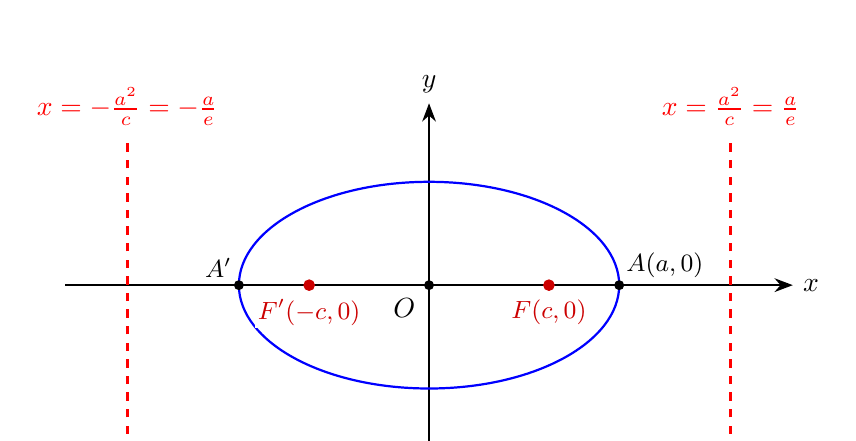
\begin{tikzpicture}[scale=1.05]
  \draw[thick, -Stealth] (-4.4, 0) -- (4.4, 0) node[right] {$x$};
  \draw[thick, -Stealth] (0, -2.0) -- (0, 2.2) node[above] {$y$};
  \filldraw (0, 0) circle (1.5pt) node[below left=2pt] {$O$};

  \draw[thick, blue] (0, 0) ellipse (2.3 and 1.25);
  \filldraw[red!80!black] (1.45, 0) circle (1.8pt) node[below=4pt, fill=white, inner sep=1pt] {\small $F(c, 0)$};
  \filldraw[red!80!black] (-1.45, 0) circle (1.8pt) node[below=4pt, fill=white, inner sep=1pt] {\small $F'(-c, 0)$};
  \filldraw (2.3, 0) circle (1.5pt) node[above right=2pt, fill=white, inner sep=1pt] {\small $A(a, 0)$};
  \filldraw (-2.3, 0) circle (1.5pt) node[above left=2pt, fill=white, inner sep=1pt] {\small $A'$};

  % Directrices
  \draw[very thick, dashed, red] (3.65, -1.8) -- (3.65, 1.8) node[above] {$x = \frac{a^2}{c} = \frac{a}{e}$};
  \draw[very thick, dashed, red] (-3.65, -1.8) -- (-3.65, 1.8) node[above] {$x = -\frac{a^2}{c} = -\frac{a}{e}$};
\end{tikzpicture}
\caption{橢圓之焦點與準線位置}
\label{fig:b4s-2-5-4}
\end{figure}

\subsubsection*{習題 2-5}
\begin{enumerate}
  \item 是否平面在圓筒面（圓柱面）上的截痕亦有類似於錐線的定理 4 的準線性質？試繪立體圖，表明其準線位置，並求其離心率與截角關係。
  \item 比較圖 \ref{fig:b4s-2-1-8} 與圖 \ref{fig:b4s-2-1-10}，其區別為前者同時固定頂點 $A$ 與兩焦點之一，後者則只固定 $A$，而讓兩焦點間距離改變。
  \begin{enumerate}[(i)]
    \item 有否方法在一固定圓錐上取截平面使截痕的一個焦點向頂點無限逼近？
    \item 欲得到一系列錐線使其中一個焦點與一個頂點距離固定，應如何調整截平面？
  \end{enumerate}
\end{enumerate}

\vspace{1.5em}
\noindent\textbf{**〔章末附註〕}\phantomsection\label{note:b4s-ch2-p96-appendix-note}

\textbf{定理 4 證明的幾何補充（$AM \perp p$ 證明）}：

自 $A$ 引 $\pi_1$ 的垂線交 $\pi_1$ 於 $R'$，再自 $R'$ 引直線 $AM$ 的垂線，垂足為 $B$。則因 $BR'$ 與 $MN$ 都垂直於 $MA$，且都在平面 $\pi_0$ 上，故 $BR' \parallel MN$。但 $MN$ 垂直於 $\pi$，故 $BR'$ 亦為 $\pi$ 的垂線。

另一方面，分別在 $\pi_1, \pi$ 上過 $R', A$ 引 $p$ 的平行直線 $l', l$，則因 $AR'$ 垂直於 $\pi_1$，故亦垂直於 $l'$，但 $l' \parallel l$，故 $AR'$ 亦垂直於 $l$。今利用三垂線定理得 $BA \perp l$，亦卽 $AM \perp p$。證畢。
 % 第二章 二次幾何 第一部分：錐線的演變
% =========================================================================
% 《高中數學實驗教材》第四冊（社會組）
% 第三章 二次幾何 第二部分：標準式
% =========================================================================

\section{二次幾何\texorpdfstring{\quad }{ }第二部分：標準式}
\label{sec:b4s-ch3}

\begin{center}
\begin{minipage}{0.75\textwidth}
\begin{itemize}[leftmargin=2em, itemsep=0.3em]
  \item[§ III-1] \textbf{橢圓}
  \begin{itemize}[leftmargin=2em, itemsep=0.2em]
    \item[甲、] 橢圓的定義與其標準式
    \item[乙、] 橢圓的形狀
    \item[丙、] 準線觀點的再證明
  \end{itemize}
  \item[§ III-2] \textbf{雙曲線}
  \begin{itemize}[leftmargin=2em, itemsep=0.2em]
    \item[甲、] 雙曲線的定義與其標準式
    \item[乙、] 雙曲線的漸近線
    \item[丙、] 雙曲線的形狀
  \end{itemize}
  \item[§ III-3] \textbf{拋物線}
  \begin{itemize}[leftmargin=2em, itemsep=0.2em]
    \item[甲、] 拋物線的定義與其標準式
    \item[乙、] 拋物線的形狀
    \item[丙、] 拋物線無漸近線
  \end{itemize}
  \item[§ III-4] \textbf{各種錐線的切線及光學性質}
  \begin{itemize}[leftmargin=2em, itemsep=0.2em]
    \item[甲、] 橢圓
    \item[乙、] 雙曲線
    \item[丙、] 拋物線
  \end{itemize}
  \item[§ III-5] \textbf{圓}
  \begin{itemize}[leftmargin=2em, itemsep=0.2em]
    \item[甲、] 圓的方程式
    \item[乙、] 圓與直線
  \end{itemize}
  \item[*§ III-6] \textbf{圓的正交與鏡射}
\end{itemize}
\end{minipage}
\end{center}

\begin{center}
$* \qquad * \qquad * \qquad * \qquad *$
\end{center}

上章我們已談過錐線，並很自然地就其形狀分為三類。更重要的是對每一類錐線剖析了它一、二特徵性質——從焦半徑的觀點或從準線的觀點。

現在我們就抽出其中較方便的特徵性質（如從正負兩類錐線抽出採取焦半徑的觀點，從零類錐線抽出準線觀點），來慎密地在平面上定義出所謂雙曲線，橢圓與拋物線，導出它們用座標描寫的標準方程式\phantomsection\label{note:b4s-ch3-biaozhunfangcheng}\footnote{【原書註記/校訂】：原書此處印作「標準友程式」，顯為「標準方程式」之排版訛字，茲予校訂。}證知它們都是一個二元二次方程式的軌跡。換句話說它們都是二次曲線\phantomsection\label{note:b4s-ch3-ercichuxian}\footnote{【原書註記/校訂】：原書此處印作「三杰典線」，字模模糊殘缺，依上下文校訂為「二次曲線」。}，如此使我們能夠求算許多（二次的）幾何性質，這樣的過程較之於第三冊的線性座標幾何\phantomsection\label{note:b4s-ch3-zuobiaojihe}\footnote{【原書註記/校訂】：原書印作「線供 標幾何」，字模脫落，依文義校訂為「線性座標幾何」；後文「上魚三次標幾何」校訂為「平面上的二次座標幾何」。}，其實就是平面上的二次座標幾何。

當然我們還是要回過頭來說明這三種二次曲線，實際上就是第二章的三類錐線，這樣的再對照，使我們了解三種二次曲線間，接續演變的情形，比如它們的焦點，它們的準線在各種二次曲線之間如何地接續地移動，使我們了解一類錐線同時能具有數種特徵性質，並非出於巧合，也使我們可以把第二章已發現的錐線性質搬過來給這些二次曲線。

在第四章，我們將要證知任何二元二次方程式所代表的曲線（卽任何二次曲線）除開特異的情形外一定是上述三種的二次曲線中的一種。

在發展理論的同時，我們嘗試提供一二，利用所得理論處理實際問題的例子，如兩貨物集散地之供應區域的範圍問題（§ III-2\phantomsection\label{note:b4s-ch3-sec-ref-2}\footnote{【原書註記/校訂】：原書此處引號誤作「§ II-2」，依目錄章節指稱校訂為「§ III-2」。}），經濟學上求最大效用的問題（§ III-4\phantomsection\label{note:b4s-ch3-sec-ref-4}\footnote{【原書註記/校訂】：原書此處印作「8II-4」，校訂為「§ III-4」。}）以及一些光學原理。這些論例的提供仍是罩在第三冊第一章所提出對實際問題與幾何代數的轉化處理，這一清晰的綱領之下。

圓是橢圓的特別情形！在自然界中尤其工程上出現的情形較多；在討論圓時，我們要再一次發揮座標幾何與向量幾何的好處。

% =========================================================================
% § III-1 橢圓
% =========================================================================
\subsection{橢圓}
\label{sec:b4s-3-1}

\subsubsection*{甲、橢圓的定義與其標準式}

在平面上取兩固定點 $F$ 與 $F'$，再取夠長的繩子，使兩端能固定於 $F, F'$ 點，然後以筆尖將繩子繃緊。此時筆尖仍可滑動（見圖 1-1）描出一條類似蛋形之曲線我們將把它叫做橢圓。

\begin{figure}[htbp]
\centering
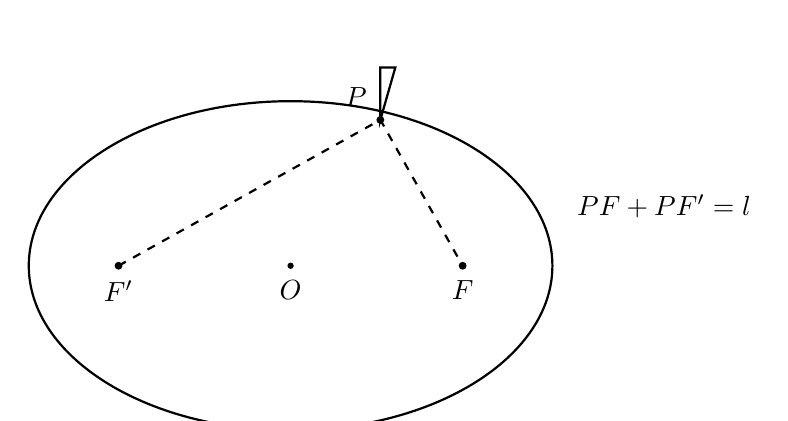
\begin{tikzpicture}[>=stealth, scale=0.95]
  % Draw ellipse
  \draw[thick] (0,0) ellipse (3.5cm and 2.2cm);
  % Foci
  \coordinate (F1) at (-2.3,0);
  \coordinate (F2) at (2.3,0);
  \coordinate (P) at (1.2, 1.95);
  \coordinate (O) at (0,0);
  \fill (O) circle (1.2pt) node[below=2pt] {$O$};
  \fill (F1) circle (1.5pt) node[below=2pt] {$F'$};
  \fill (F2) circle (1.5pt) node[below=2pt] {$F$};
  \fill (P) circle (1.5pt) node[above left=2pt] {$P$};
  % Strings
  \draw[thick, dashed] (F1) -- (P) -- (F2);
  % Pencil tip sketch
  \draw[thick] (P) -- ++(0.2, 0.7) -- ++(-0.2, 0) -- cycle;
  % Condition label on the right
  \node[right] at (3.7, 0.8) {$PF + PF' = l$};
\end{tikzpicture}
\caption{橢圓的繪法}
\label{fig:b4s-3-1}
\end{figure}

\begin{definition*}
平面上到兩固定點 $F$ 與 $F'$ 之距離和為一定長 $l$ 的點所組成的曲線，稱為\textbf{橢圓}，其中 $l > \overline{FF'}$，通常 $F$ 與 $F'$ 稱為橢圓的兩個\textbf{焦點}。線段 $FF'$ 之中點 $O$ 稱為\textbf{橢圓中心}。

換句話說：對平面上一曲線 $\Gamma_-$，如存在兩點 $F$ 及 $F'$，一方面（不一定相異）使這曲線 $\Gamma_-$ 上的任一點 $P$ 滿足
\begin{equation}
PF + PF' = \text{定長} \label{eq:b4s-3-1-1}
\end{equation}
另一方面使任何滿足上式的點 $P$ 都在這曲線 $\Gamma_-$ 上，則這曲線 $\Gamma_-$ 稱為一個橢圓。$PF$ 與 $PF'$ 稱為過 $P$ 的兩個\textbf{焦半徑}。
\end{definition*}

從這個定義，我們注意到橢圓由 $F, F'$ 之位置及尺長 $l$ 完全決定。若不計橢圓之位置，只計其形狀大小，則橢圓由長度 $\overline{FF'}$ 及 $l$ 完全決定。

這一性質很顯然是負類錐線的一個特徵性質，因此負類錐線都是橢圓，至於它的反命題將在乙段說明。設 $\Gamma_-$ 為一已知橢圓，$F, F'$ 為兩焦點，$O$ 為其中心，今連結 $FF'$，得一直線 $L$，在 $L$ 上 $F$ 與 $F'$ 按序分居於 $O$ 的右與左兩側，如圖 1-2。設 $A$ 點為這橢圓 $\Gamma_-$ 的一個交點而以 $a$ 表 $O$ 到 $A$ 的距離 $OA$。先考慮 $A$ 與 $F$ 同在 $O$ 的右側這一情況，此時 $A$ 更落在 $F$ 的右側〔不然，則 $AF + AF' = FF' < l$ 不符合 $A$ 在 $\Gamma_-$ 上的假定〕。

\begin{figure}[htbp]
\centering
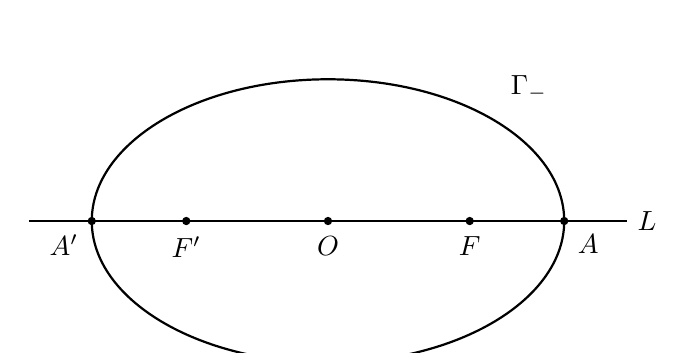
\begin{tikzpicture}[>=stealth, scale=1.0]
  \draw[thick] (-3.8,0) -- (3.8,0) node[right] {$L$};
  \coordinate (O) at (0,0);
  \coordinate (F1) at (-1.8,0);
  \coordinate (F2) at (1.8,0);
  \coordinate (A1) at (-3.0,0);
  \coordinate (A2) at (3.0,0);
  \fill (O) circle (1.5pt) node[below=2pt] {$O$};
  \fill (F1) circle (1.5pt) node[below=2pt] {$F'$};
  \fill (F2) circle (1.5pt) node[below=2pt] {$F$};
  \fill (A1) circle (1.5pt) node[below left=2pt] {$A'$};
  \fill (A2) circle (1.5pt) node[below right=2pt] {$A$};
  \draw[thick] (0,0) ellipse (3.0cm and 1.8cm);
  \node[above right] at (2.2, 1.4) {$\Gamma_-$};
\end{tikzpicture}
\caption{橢圓頂點與焦點}
\label{fig:b4s-3-2}
\end{figure}

今
\begin{align*}
l &= AF + AF' \\
  &= AF + (AO + OF') \quad \text{〔因 $A$ 與 $F'$ 分居於 $O$ 的兩側〕} \\
  &= (AF + FO) + AO \quad \text{〔因 $OF' = FO$〕} \\
  &= AO + AO = 2a \quad \text{〔因 $A$ 與 $O$ 分居於 $F$ 之兩側〕}
\end{align*}
同理，若 $A'$ 與 $F'$ 同在 $O$ 的左側，亦得 $l = 2a$，故橢圓 $\Gamma_-$ 與 $L$ 確有兩交點 $A, A'$ 分別處於 $F$ 的右側與 $F'$ 的左側，且 $A$ 與 $A'$ 到 $O$ 的距離等長，其值為 $a$。

當我們想取一直角座標系使橢圓的方程式成一最簡潔的形式時，上述的討論自然也提示我們選線段 $F'F$ 的中點 $O$ 為原點，而選直線 $F'F$ 為 $x$ 軸，對於這樣的一個正交座標系 $(O; X, Y)$，我們可取兩實數 $a$ 與 $c \ge 0$，使 $F, F', A, A'$ 各點座標為
\[ A'(-a,0), \quad F'(-c,0), \quad F(c,0), \quad A(a,0) \]
注意：因 $l > \overline{FF'}$，而 $l = 2a, \overline{FF'} = 2c$，故 $a > c$。

\begin{definition*}
線段 $AA'$ 稱為橢圓之\textbf{長軸}，其長之半 $a = \frac{1}{2}\overline{AA'}$ 稱為\textbf{長軸半長}，橢圓 $\Gamma_-$ 的\textbf{離心率} $e$ 為
\[ e = \frac{\overline{FF'}}{\overline{AA'}} = \frac{c}{a} \]
卽知 $0 \le e < 1$\phantomsection\label{note:b4s-ch3-e-circle}\footnote{〔原書註〕$e=0$ 表示焦距 $c=0$，即二焦點重合，此時 $a=b=\frac{1}{2}l$ 而圖形為一圓。圓是橢圓的特異情形，稍後將特別討論圓。}。
\end{definition*}

\begin{figure}[htbp]
\centering
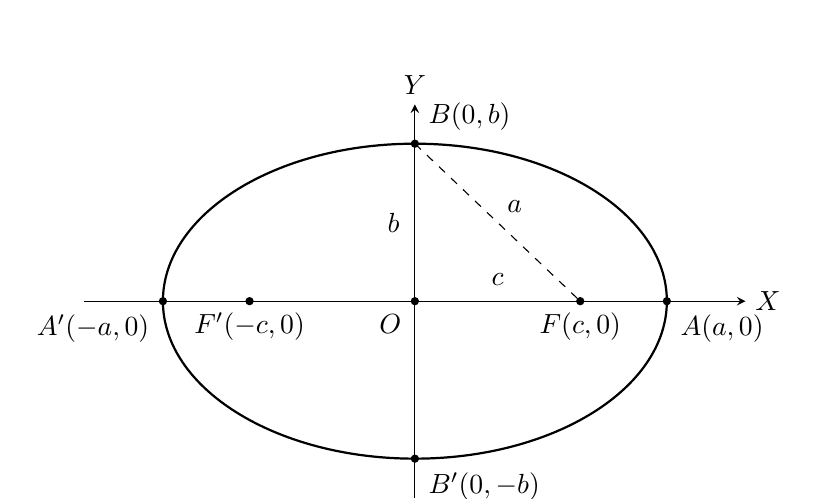
\begin{tikzpicture}[>=stealth, scale=1.0]
  \draw[->] (-4.2,0) -- (4.2,0) node[right] {$X$};
  \draw[->] (0,-2.5) -- (0,2.5) node[above] {$Y$};
  \draw[thick] (0,0) ellipse (3.2cm and 2.0cm);
  \coordinate (O) at (0,0);
  \coordinate (F1) at (-2.1,0);
  \coordinate (F2) at (2.1,0);
  \coordinate (A1) at (-3.2,0);
  \coordinate (A2) at (3.2,0);
  \coordinate (B1) at (0,2.0);
  \coordinate (B2) at (0,-2.0);
  \fill (O) circle (1.5pt) node[below left=2pt] {$O$};
  \fill (F1) circle (1.5pt) node[below=3pt, fill=white, inner sep=1pt] {$F'(-c,0)$};
  \fill (F2) circle (1.5pt) node[below=3pt, fill=white, inner sep=1pt] {$F(c,0)$};
  \fill (A1) circle (1.5pt) node[below left=2pt] {$A'(-a,0)$};
  \fill (A2) circle (1.5pt) node[below right=2pt] {$A(a,0)$};
  \fill (B1) circle (1.5pt) node[above right=2pt] {$B(0,b)$};
  \fill (B2) circle (1.5pt) node[below right=2pt] {$B'(0,-b)$};
  \draw[dashed] (B1) -- (F2) node[midway, above right] {$a$};
  \node[above=2pt] at (1.05, 0) {$c$};
  \node[left=2pt] at (0, 1.0) {$b$};
\end{tikzpicture}
\caption{橢圓與正交座標系}
\label{fig:b4s-3-3}
\end{figure}

另一方面，設 $B(0,b)$ 為橢圓 $\Gamma_-$ 與 $Y$ 軸的交點，則 $BF + BF' = l = 2a$。但 $Y$ 軸為線段 $FF'$ 之中垂線故 $BF = BF' = a$，遂知
\[ b^2 = a^2 - c^2 \]
因此 $b = \sqrt{a^2 - c^2}$，亦卽橢圓 $\Gamma_-$ 截 $Y$ 軸於兩點 $B(0,b)$ 與 $B'(0,-b)$。線段 $BB'$ 稱為橢圓的\textbf{短軸}，$b$ 稱為\textbf{短軸半長}，$A, A', B, B'$ 稱為橢圓的\textbf{頂點}。

這時候我們已可由這四點 $A, A', B, B'$ 得到了「由到兩定點距離和為定長之點」這一軌跡（卽所謂橢圓）的大體輪廓，進一步，我們要準確地以方程式來表示這一軌跡。

\begin{proposition}
給定一橢圓 $\Gamma_-$ 可取一正交座標系 $(O; \mathbf{e}_1, \mathbf{e}_2)$ 使橢圓中心為原點 $(0,0)$，兩焦點為 $F(c,0), F'(-c,0)$，長軸長為 $2a$，則橢圓的方程式為
\begin{equation}
\Gamma_- : \frac{x^2}{a^2} + \frac{y^2}{b^2} = 1 \label{eq:b4s-3-1-2}
\end{equation}
其中 $b = \sqrt{a^2 - c^2}$。
\end{proposition}

\begin{figure}[htbp]
\centering
\begin{tikzpicture}[>=stealth, scale=0.95]
  \draw[->] (-4,0) -- (4,0) node[right] {$x$};
  \draw[->] (0,-2.5) -- (0,2.5) node[above] {$y$};
  \draw[thick] (0,0) ellipse (3.2cm and 1.9cm);
  \coordinate (O) at (0,0);
  \coordinate (F1) at (-2.0,0);
  \coordinate (F2) at (2.0,0);
  \coordinate (P) at (1.8, 1.45);
  \fill (O) circle (1.2pt) node[below left=2pt] {$O$};
  \fill (F1) circle (1.5pt) node[below=2pt, fill=white, inner sep=1pt] {$F'(-c,0)$};
  \fill (F2) circle (1.5pt) node[below=2pt, fill=white, inner sep=1pt] {$F(c,0)$};
  \fill (P) circle (1.5pt) node[above right=2pt] {$P(x,y)$};
  \draw[thick] (F1) -- (P) -- (F2);
\end{tikzpicture}
\caption{橢圓上一點與兩焦點}
\label{fig:b4s-3-3prime}
\end{figure}

\begin{proof}
設 $P(x,y)$ 為 $\Gamma_-$ 上的一般點，則因 $PF + PF' = 2a$，推得
\begin{equation}
\sqrt{(x-c)^2 + y^2} + \sqrt{(x+c)^2 + y^2} = 2a \notag
\end{equation}
移項得
\[ \sqrt{(x-c)^2 + y^2} = 2a - \sqrt{(x+c)^2 + y^2} \]
兩端平方得
\[ (x-c)^2 + y^2 = 4a^2 - 4a\sqrt{(x+c)^2 + y^2} + (x+c)^2 + y^2 \]
稍加整理，得
\begin{equation}
a\sqrt{(x+c)^2 + y^2} = a^2 + cx \label{eq:b4s-3-1-3}
\end{equation}
兩端再作平方：
\[ a^2[(x+c)^2 + y^2] = (a^2 + cx)^2 = a^4 + 2a^2cx + c^2x^2 \]
展開化簡：
\[ a^2x^2 + 2a^2cx + a^2c^2 + a^2y^2 = a^4 + 2a^2cx + c^2x^2 \]
\begin{equation}
(a^2 - c^2)x^2 + a^2y^2 = a^2(a^2 - c^2) \label{eq:b4s-3-1-4}
\end{equation}
以 $b^2 = a^2 - c^2$ 代入得
\[ b^2x^2 + a^2y^2 = a^2b^2 \]
除以 $a^2b^2$：
\[ \frac{x^2}{a^2} + \frac{y^2}{b^2} = 1 \]
\end{proof}

取適當的正交座標系，橢圓這一看似複雜的曲線竟以 \eqref{eq:b4s-3-1-2} 式這簡潔的形式出現，這個 \eqref{eq:b4s-3-1-2} 式我們就稱為橢圓的\textbf{標準式}。

注意在 \eqref{eq:b4s-3-1-2} 式的導引過程中，作了兩次平方，照理可能會產生很多不見得仍滿足原來關係式
\[ PF + PF' = 2a \]
的點 $(x,y)$。第一次作平方後實際上考慮的已經是滿足
\[ \pm PF \pm PF' = 2a \]
的所有點 $(x,y)$ 了。第二次再作平方，所考慮的點更增多到所有滿足
\[ \pm PF \pm PF' = \pm 2a \]
的 $(x,y)$，其中左右兩端的 $\pm$ 號可以分配為 $(+,+), (+,-), (-,+), (-,-)$ 等四種可能。而我們的式子只不過是第二種 $(+,-)$ 的情形：
今分述其餘三種情形如下：
\begin{enumerate}[(i)]
  \item $(-,+)$ 的情形，因 $2a > 0$ 故不可能發生。
  \item $(+,+)$ 與 $(-,-)$ 的情形，其實可合寫為 $|PF - PF'| = 2a > 2c = FF'$，上式表示三角形 $\triangle PFF'$ 兩邊之差會大於第三邊，此為不可能故不致產生這樣的 $P(x,y)$ 點。
\end{enumerate}
故平方過程所可能引進的多餘軌跡其實均不存在，換言之，方程式 \eqref{eq:b4s-3-1-2} 的實數解恰好就是橢圓上的點。

標準式 \eqref{eq:b4s-3-1-2} 雖然看似代表某一種特殊的橢圓，但是如果我們不計較橢圓的位置，只考慮它的形狀與大小，標準式這種形式的方程式實際上卻是描寫了所有的橢圓。

\begin{example}
如橢圓中心不在已給自然座標系的原點，而在點 $(1,1)$，兩焦點座標分別為 $F=(2,1), F'=(0,1)$，長軸半長為 2，則此橢圓的方程式為何？

\begin{figure}[htbp]
\centering
\begin{tikzpicture}[>=Stealth, scale=1.1]
  \draw[->] (-1.5,0) -- (4.2,0) node[right] {$x$};
  \draw[->] (0,-1) -- (0,3.5) node[above] {$y$};
  \coordinate (O) at (0,0);
  \coordinate (O1) at (1,1);
  \coordinate (F1) at (0,1);
  \coordinate (F2) at (2,1);
  \draw[dashed] (-1.2,1) -- (3.8,1) node[right] {$y=1$};
  \draw[dashed] (1,-0.8) -- (1,3.2) node[above] {$x=1$};
  \draw[thick] (1,1) ellipse (2.0cm and 1.732cm);
  \fill (O) circle (1.2pt) node[below left=2pt, fill=white, inner sep=1pt] {$O$};
  \fill (O1) circle (1.5pt) node[below right=2pt, fill=white, inner sep=1pt] {\small $O'(1,1)$};
  \fill (F1) circle (1.5pt) node[above left=2pt, fill=white, inner sep=1pt] {\small $F'(0,1)$};
  \fill (F2) circle (1.5pt) node[above right=2pt, fill=white, inner sep=1pt] {\small $F(2,1)$};
\end{tikzpicture}
\caption{中心在 $(1,1)$ 的橢圓}
\label{fig:b4s-3-4}
\end{figure}

\textbf{解 1}\quad 設 $P(x,y)$ 為 $\Gamma_-$ 上的一般點，則由橢圓定義：
\[ PF + PF' = 2 \times 2 = 4 \]
卽
\[ \sqrt{(x-2)^2 + (y-1)^2} + \sqrt{x^2 + (y-1)^2} = 4 \]
兩端平方，得
\[ \sqrt{x^2 + (y-1)^2} = 2 + \frac{1}{2}x \]
再平方得
\[ 4[x^2 + (y-1)^2] = (4 + x)^2 = 16 + 8x + x^2 \]
配方整理得：
\[ 3(x-1)^2 + 4(y-1)^2 = 12 \]
注意：此橢圓的長軸在 $y-1=0$ 上，平行於 $X$ 軸，短軸則在 $x-1=0$，且 $a=2, c=1$，故 $b^2 = a^2 - c^2 = 4-1 = 3$，故上式的形式，其實就是
\[ \frac{(x-1)^2}{4} + \frac{(y-1)^2}{3} = 1 \]

\textbf{解 2}\quad 取一正交座標系 $S$ 使 $O'=(1,1)$ 為 $S$ 的原點，原基底為 $S$ 的基底，則 $F=(2,1) = (1,0)_S$，$F'=(0,1) = (-1,0)_S$。因 $c = \overline{O'F} = 1, a = 2$，故 $b = \sqrt{3}$；故可得相關於 $S$ 的橢圓表示式為
\[ \frac{X^2}{4} + \frac{Y^2}{3} = 1 \]
因新舊座標的關係為：$X = x-1, Y = y-1$，故根據原自然座標系橢圓方程式為：
\[ \frac{(x-1)^2}{4} + \frac{(y-1)^2}{3} = 1 \]
此與解 1 所得的形式相同。我們有時也稱此類的形式為\textbf{準標準形}，因為可以從此形式中，直截看出圖形為橢圓，且定出中心位置及長短軸的大小。（注意標準式中無 $xy$ 項）
\end{example}

\begin{exercise}
\begin{enumerate}[(i)]
  \item 設橢圓中心為 $(1,1)$，兩焦點座標分別為 $F=(1,0), F'=(1,2)$，長軸長為 4，試求此橢圓方程式。如何寫成標準式？
  \item 當 $b > a > 0$ 時，$\frac{x^2}{a^2} + \frac{y^2}{b^2} = 1$ 之圖形為何？焦點位置為何？
  \item 試證中心在 $(h,k)$，兩焦點為 $F(h+c, k), F'(h-c, k)$，半長軸為 $a$ 的橢圓方程式為
  \[ \frac{(x-h)^2}{a^2} + \frac{(y-k)^2}{a^2 - c^2} = 1 \]
  \item 設 $F=(1,1), F'=(0,-1)$，$PF + PF' = 3$，試求滿足上述條件的點 $P$ 所形成的橢圓方程式，並注意所得的方程式能否寫成前文所述的準標準型？（例如用配方法）（提示：在自然座標系中不可能，到第四章我們將講述如何用固有值的方法，求得一新正交座標系而將橢圓的方程式化成標準型。）
\end{enumerate}
\end{exercise}

\subsubsection*{乙、橢圓的形狀}

講到橢圓的形狀能否加以「數量化」，亦卽能否以幾個數量來決定它的形狀？這便觸及數學的一個主要精神。標準式 \eqref{eq:b4s-3-1-2} 其實已相當程度告訴了我們 $a$ 與 $b$ 是怎樣的兩個數量，但讓我們更原始地來看這一問題。在前面定義過橢圓之後，我們馬上提出它可由 $F, F'$ 的位置及定長 $l$ 決定。現在當我們不計較橢圓位置，而只看它的形狀時，決定的因素實際上便只是長度 $\overline{FF'}$ 與 $l$ 而已，但
\[ c = \frac{1}{2}\overline{FF'}, \quad a = \frac{1}{2}l \]
故決定的因素亦可視為 $a$ 與 $c$，$\{a, c\}$ 二值可作為決定橢圓的一組資料。更進一層，因離心率 $e = \frac{c}{a}$，故若知 $e$ 與 $a$，則知 $c = ae$，便知橢圓之形狀，卽二數 $\{a, e\}$ 亦為決定橢圓的一組資料。若 $e \neq 0$ 則 $\{a, e\}$ 與 $\{a, c\}$ 這兩組資料相互決定，我們稱 $\{a, e\}$ 與 $\{a, c\}$ 為等價的資料。

就幾何意義來說，我們較易用離心率 $e$ 與長軸長 $a$ 來看出橢圓形狀的變化，離心率 $e$ 決定扁的程度：固定 $a$ 則 $e$ 越大橢圓越扁；而 $a$ 決定其大小：固定 $e$ 則當 $a$ 增加，橢圓亦隨比例相似地擴大（見圖 1-5）。

\begin{figure}[htbp]
\centering
\begin{tikzpicture}[>=Stealth, scale=0.76]
  % Left: a fixed = 4, e varies
  \begin{scope}[xshift=-5.3cm]
    \node[anchor=west] at (-4.2, 4.3) {\small ($a$ 固定為 4)};
    \draw[->] (-4.5,0) -- (4.6,0) node[right] {$x$};
    \draw[->] (0,-4.0) -- (0,4.3) node[above] {$y$};
    \draw[thick] (0,0) ellipse (4cm and 3.66cm); % e=0.4
    \node[fill=white, inner sep=1pt] at (1.8, 3.35) {\footnotesize $e=0.4$};
    \draw[thick, dashed] (0,0) ellipse (4cm and 2.85cm); % e=0.7
    \node[fill=white, inner sep=1pt] at (1.8, 2.55) {\footnotesize $e=0.7$};
    \draw[thick, dotted] (0,0) ellipse (4cm and 1.74cm); % e=0.9
    \node[fill=white, inner sep=1pt] at (1.8, 1.55) {\footnotesize $e=0.9$};
  \end{scope}
  % Right: e fixed = 0.8, a varies
  \begin{scope}[xshift=5.3cm]
    \node[anchor=west] at (-4.2, 4.3) {\small ($e$ 固定為 0.8)};
    \draw[->] (-4.5,0) -- (4.6,0) node[right] {$x$};
    \draw[->] (0,-3.2) -- (0,3.6) node[above] {$y$};
    % e=0.8, b/a = sqrt(1-0.64) = 0.6
    \draw[thick] (0,0) ellipse (1.8cm and 1.08cm); % a=3
    \node[fill=white, inner sep=1pt] at (1.05, 0.92) {\footnotesize $a=3$};
    \draw[thick, dashed] (0,0) ellipse (3.0cm and 1.8cm); % a=5
    \node[fill=white, inner sep=1pt] at (1.55, 1.58) {\footnotesize $a=5$};
    \draw[thick, dotted] (0,0) ellipse (4.2cm and 2.52cm); % a=7
    \node[fill=white, inner sep=1pt] at (2.1, 2.25) {\footnotesize $a=7$};
  \end{scope}
\end{tikzpicture}
\caption{離心率與長軸對橢圓形狀的影響}
\label{fig:b4s-3-5}
\end{figure}

\begin{example}
設二橢圓 $\Gamma_-$ 與 $\Gamma_-'$ 各由 $\{e, a\}$ 與 $\{e, a'\}$ 決定，其中 $e$ 為離心率，$a, a'$ 為長軸半長，試證 $\Gamma_-$ 與 $\Gamma_-'$ 相似，亦卽若取 $\lambda = \frac{a'}{a}$，則在平面上作適當之剛性運動使二橢圓之中心與對稱軸重合後，有
\[ (x,y) \in \Gamma_- \iff (\lambda x, \lambda y) \in \Gamma_-' \]

\begin{proof}
因形狀大小與位置無關，可將二橢圓中心重合，取為原點，且長軸均重合於 $X$ 軸，則二橢圓之標準式各為
\[ \Gamma_- : \frac{x^2}{a^2} + \frac{y^2}{b^2} = 1, \quad \text{其中 } b = a\sqrt{1-e^2} \]
\[ \Gamma_-' : \frac{x^2}{a'^2} + \frac{y^2}{b'^2} = 1, \quad \text{其中 } b' = a'\sqrt{1-e^2} \]
若設 $\lambda = \frac{a'}{a}$，則 $a' = \lambda a, b' = \lambda b$，將 $(\lambda x, \lambda y)$ 代入 $\Gamma_-'$ 得
\[ \frac{(\lambda x)^2}{(\lambda a)^2} + \frac{(\lambda y)^2}{(\lambda b)^2} = \frac{\lambda^2 x^2}{\lambda^2 a^2} + \frac{\lambda^2 y^2}{\lambda^2 b^2} = \frac{x^2}{a^2} + \frac{y^2}{b^2} = 1 \]
故 $(\lambda x, \lambda y) \in \Gamma_-' \iff (x,y) \in \Gamma_-$，我們稱 $\Gamma_-'$ 為 $\Gamma_-$ 的 $\lambda$ 倍放大。
\end{proof}
\end{example}

\begin{example}[橢圓之伸縮作圖]
求作 $\frac{x^2}{16} + \frac{y^2}{4} = 1$ 之圖形。

\textbf{解}\quad 將方程式兩邊乘以 4，使 $y^2$ 項的係數為 1，則方程式變成
\begin{equation}
\frac{x^2}{4} + y^2 = 4 \quad \text{卽} \quad \left(\frac{x}{2}\right)^2 + y^2 = 2^2 \label{eq:b4s-3-ex3}
\end{equation}
若設 $x' = \frac{x}{2}, y' = y$，則上式可寫成
\[ x'^2 + y'^2 = 2^2 \]
這對 $(x', y')$ 而言為以原點為心，半徑等於 2 之圓（見圖 1-6a）。因 $x = 2x'$，故將此圓圖形的橫軸方向放大 2 倍，卽得原橢圓之圖形（見圖 1-6b）。

\begin{figure}[htbp]
\centering
\begin{tikzpicture}[>=Stealth, scale=0.78]
  % 1-6a
  \begin{scope}[xshift=-4.4cm]
    \draw[->] (-3,0) -- (3,0) node[right] {$x'$};
    \draw[->] (0,-3) -- (0,3) node[above] {$y'$};
    \draw[thick] (0,0) circle (2cm);
    \node[below left=2pt] at (0,0) {$O$};
    \node[below right=2pt] at (2,0) {$2$};
    \node[above left=2pt] at (0,2) {$2$};
    \node at (0, -3.4) {圖 1-6a};
  \end{scope}
  % 1-6b
  \begin{scope}[xshift=4.2cm]
    \draw[->] (-4.5,0) -- (4.5,0) node[right] {$x$};
    \draw[->] (0,-3) -- (0,3) node[above] {$y$};
    \draw[thick] (0,0) ellipse (4cm and 2cm);
    \node[below left=2pt] at (0,0) {$O$};
    \node[below right=2pt] at (4,0) {$4$};
    \node[above left=2pt] at (0,2) {$2$};
    \node at (0, -3.4) {圖 1-6b};
  \end{scope}
\end{tikzpicture}
\caption{橢圓之伸縮作圖法}
\label{fig:b4s-3-6}
\end{figure}
\end{example}

\begin{exercise}
仿上述論例求作 $\frac{x^2}{9} + \frac{y^2}{25} = 1$ 之圖形。
\end{exercise}

\begin{example}
各行星相對於太陽的軌道為橢圓，其離心率及平均軌道半徑列表如下：
\begin{center}
\begin{tabular}{|c|c|c|c|}
\hline
行星 & 離心率 $e$ & 平均軌道半徑（$\text{AU}$） & 週期（日） \\ \hline
水星 & 0.206 & 0.389 & 87.77 \\ \hline
金星 & 0.007 & 0.724 & 224.70 \\ \hline
地球 & 0.017 & 1.000 & 365.25 \\ \hline
火星 & 0.093 & 1.524 & 686.98 \\ \hline
木星 & 0.048 & 5.200 & 4332.62 \\ \hline
土星 & 0.056 & 9.510 & 10789.20 \\ \hline
天王星 & 0.047 & 19.191 & 30685.93 \\ \hline
海王星 & & & \\ \hline
冥王星 & & & \\ \hline
\end{tabular}
\end{center}
其中所謂平均軌道半徑為行星至太陽最遠與最近距離之平均值，這平均軌道半徑也就是長軸半長 $a$。（我們取地球至太陽的平均軌道半徑為一天文單位 astronomical unit，簡記以 $\text{AU}$。）

設行星的橢圓軌道方程式為：$\frac{x^2}{a^2} + \frac{y^2}{b^2} = 1$，式中太陽在 $F(c,0)$ 處，最近點與最遠點分別為 $A, A'$，則 $A=(a,0), A'=(-a,0)$，故平均軌道半徑應為 $(a-c)$ 與 $(a+c)$ 之平均值，卽等於 $a$。今取火星為例，其離心率為 $e = 0.093$，平均軌道半徑 $a = 1.524\text{ AU}$，則
\[ c = ae = 1.524 \times 0.093 = 0.141732\text{ AU} \]
則最近與最遠距離分別為
\[ a - c = 1.382268\text{ AU}, \qquad a + c = 1.665732\text{ AU} \]

\begin{figure}[htbp]
\centering
\begin{tikzpicture}[>=stealth, scale=1.0]
  \draw[thick] (0,0) ellipse (3.5cm and 2.5cm);
  \coordinate (Sun) at (1.2,0);
  \coordinate (A) at (3.5,0);
  \coordinate (Aprime) at (-3.5,0);
  \fill[orange!90!black] (Sun) circle (3.5pt) node[below=4pt] {太陽 $F$};
  \fill (A) circle (2pt) node[right=3pt] {近日點（行星）};
  \fill (Aprime) circle (2pt) node[left=3pt] {遠日點};
  % Dimension lines above
  \draw[<->] ($(Sun)+(0,0.8)$) -- ($(A)+(0,0.8)$) node[midway, fill=white, inner sep=1pt] {$a-c$};
  \draw[<->] ($(Aprime)+(0,0.8)$) -- ($(Sun)+(0,0.8)$) node[midway, fill=white, inner sep=1pt] {$a+c$};
  \draw[dotted] (Sun) -- ($(Sun)+(0,0.8)$);
  \draw[dotted] (A) -- ($(A)+(0,0.8)$);
  \draw[dotted] (Aprime) -- ($(Aprime)+(0,0.8)$);
\end{tikzpicture}
\caption{行星繞日橢圓軌道}
\label{fig:b4s-3-7}
\end{figure}
\end{example}

\begin{exercise}
何以行星到太陽的最近點與最遠點分別為其橢圓軌道之長軸上的兩頂點？九大行星中哪一行星軌道最扁，次扁？哪一行星軌道最近於正圓？
\end{exercise}

\begin{exercise}
仿論例 3 作圖法，描繪水星、土星、海王星之軌道。
\end{exercise}

\begin{exercise}
\begin{enumerate}[(i)]
  \item 固定 $a=5$，試大略繪出 $e=0.4, 0.7, 0.9$ 的橢圓曲線。
  \item 固定 $a=2$，而讓 $e$ 變動寫出相應的橢圓系，卽一系列的橢圓的方程式，並作圖表明其隨 $e$ 變化的情形。〔提示：在 $\Gamma_- : \frac{x^2}{a^2} + \frac{y^2}{b^2} = 1$ 中，$b^2 = a^2(1-e^2)$〕
  \item 已知 $e = \frac{3}{5}$，試大略繪出半長軸為 $5, 7, 10$ 時的橢圓曲線。
  \item 固定 $e = \frac{1}{2}$ 而讓 $a$ 變動，寫出其相應的橢圓系方程式，並作圖表明其隨 $a$ 變化的變化。
  \item 固定 $c=1$，而讓 $a$ 變動寫出相應的橢圓方程式，當 $a$ 趨於 $c$ 時，橢圓的極限位置為何？
\end{enumerate}
\end{exercise}

利用離心率與長軸半長，我們便可以說明一項重要事實。

\begin{proposition}
橢圓其實就是負類錐線。
\end{proposition}

\begin{proof}[說明]
「兩焦半徑之和為定長」據定義便是橢圓，而負類錐線在第二章中已證得有此特徵性質，故負類錐線必為一橢圓。反過來給定一橢圓 $\Gamma_-$ 設其離心率為 $e_0$，長軸半長為 $a_0$，我們要找出一負類錐線 $\Gamma$ 使兩曲線 $\Gamma_-$ 與 $\Gamma$ 的形狀一致：
\begin{enumerate}[(i)]
  \item 取一固定圓錐 $\Omega$，其頂角 $\alpha$，設一平面 $\pi$ 在 $\Omega$ 上的截角為 $\theta$ ($0 < \theta < \alpha'$)，在第二章已導得截痕 $\Gamma$ 之離心率為
  \[ e = \frac{\sin\theta}{\sin\alpha'} \]
  現在取截角 $\theta$ 為 $\theta_0$ 使 $\sin\theta_0 = e_0 \sin\alpha'$。這是辦得到的，道理是：$0 \le e_0 < 1$ 且當 $\theta$ 從 $0$ 變化到 $\alpha'$ 時，$\frac{\sin\theta}{\sin\alpha'}$ 之值亦從 $0$ 變化到 $1$，故必有某 $\theta_0$ 使比值等於已給的 $e_0$。這樣相應於截角為 $\theta_0$ 時的負類錐線 $\Gamma$ 的離心率便為 $e_0$。
  \item 所剩的便是調整 $\Gamma$ 的大小。將 $\Gamma$ 所在的截面 $\pi$ 上下平行移動（見圖 1-8），藉以調整其長軸，則因這樣的移動，使其長軸半長範圍從 $0$ 伸向 $\infty$，故必得一平面 $\pi$ 其長軸之半長為 $a_0$。
\end{enumerate}
對於這樣取得的 $\pi$，其截在 $\Omega$ 上的錐線因已知為一橢圓，且其離心率及其長軸半長皆與已給定的橢圓 $\Gamma_-$ 的離心率 $e_0$ 與長軸半長 $a_0$ 吻合，卽 $\Gamma_-$ 成為一負類錐線。
\end{proof}

\begin{figure}[htbp]
\centering
\begin{tikzpicture}[>=stealth, scale=0.9]
  % Cone
  \coordinate (V) at (0,2.5);
  \draw[thick] (-2.5,-3) -- (V) node[above] {$K$} -- (2.5,-3);
  \draw[dashed] (0,2.5) -- (0,-3.2);
  % Elliptic sections parallel
  \draw[thick, fill=blue!5, fill opacity=0.3, rotate around={-25:(0,0.8)}] (0,0.8) ellipse (1.1cm and 0.45cm);
  \draw[thick, fill=blue!10, fill opacity=0.3, rotate around={-25:(0,-1.2)}] (0,-1.2) ellipse (2.1cm and 0.85cm);
  \node[right] at (1.1, 0.4) {$\pi$};
  \node[right] at (2.0, -1.6) {$\pi'$};
  \draw[->, thick] (1.3, -0.6) -- (1.3, 0.4) node[midway, right] {平行移動};
\end{tikzpicture}
\caption{圓錐截面之平行移動}
\label{fig:b4s-3-8}
\end{figure}

從這一事實，我們更能把負類錐線所有已知的性質，都搬過來給橢圓。例如，根據準線觀點，那時已證得定理 I，現在我們也得到：

\begin{theorem}
給定一橢圓
\[ \Gamma_- : \frac{x^2}{a^2} + \frac{y^2}{b^2} = 1 \qquad (a > b > 0) \]
則存在兩直線（稱為橢圓 $\Gamma_-$ 的二準線）
\[ p: x = \frac{a^2}{c}, \qquad p': x = -\frac{a^2}{c} \]
使 $\Gamma_-$ 上任意 $P(x,y)$ 到焦點距離 $PF$（或 $PF'$）與到 $p$（或 $p'$）的距離 $PT$（或 $PT'$）為一定比，且這定比等於 $\Gamma_-$ 的離心率，亦卽
\begin{equation}
\frac{PF}{PT} = \frac{PF'}{PT'} = e \label{eq:b4s-3-1-5}
\end{equation}
\end{theorem}

\subsubsection*{丙、準線觀點的再證明}

我們不妨在平面上利用座標幾何的方法，將上述的定理 I 重作證明如下：

\begin{figure}[htbp]
\centering
\begin{tikzpicture}[>=stealth, scale=1.0]
  \draw[->] (-4.5,0) -- (4.5,0) node[right] {$x$};
  \draw[->] (0,-2.5) -- (0,2.5) node[above] {$y$};
  \draw[thick] (0,0) ellipse (3.0cm and 1.8cm);
  \coordinate (O) at (0,0);
  \coordinate (F1) at (-1.8,0);
  \coordinate (F2) at (1.8,0);
  \coordinate (P) at (1.5, 1.56);
  \coordinate (T) at (3.8, 1.56);
  % Directrices
  \draw[thick, dashed] (3.8,-2.5) -- (3.8,2.5) node[above, fill=white, inner sep=1pt] {$p: x = \frac{a^2}{c}$};
  \draw[thick, dashed] (-3.8,-2.5) -- (-3.8,2.5) node[above, fill=white, inner sep=1pt] {$p': x = -\frac{a^2}{c}$};
  \fill (O) circle (1.2pt) node[below left=2pt] {$O$};
  \fill (F1) circle (1.5pt) node[below=2pt, fill=white, inner sep=1pt] {$F'(-c,0)$};
  \fill (F2) circle (1.5pt) node[below=2pt, fill=white, inner sep=1pt] {$F(c,0)$};
  \fill (P) circle (1.5pt) node[above left=2pt] {$P(x,y)$};
  \fill (T) circle (1.5pt) node[above right=2pt] {$T$};
  \draw[thick] (F2) -- (P);
  \draw[thick] (P) -- (T);
  % Right angle mark at T
  \draw ($(T)+(-0.2,0)$) |- ($(T)+(0,-0.2)$);
\end{tikzpicture}
\caption{橢圓與準線}
\label{fig:b4s-3-9}
\end{figure}

\begin{proof}
設 $P(x,y)$ 為橢圓 $\Gamma_- : \frac{x^2}{a^2} + \frac{y^2}{b^2} = 1$ 上一點，則
\begin{equation}
y^2 = b^2\left(1 - \frac{x^2}{a^2}\right) = (a^2 - c^2)\left(1 - \frac{x^2}{a^2}\right) \label{eq:b4s-3-1-6}
\end{equation}
而 $P$ 到 $p: x = \frac{a^2}{c}$ 的距離為
\[ PT = \left|\frac{a^2}{c} - x\right| = \frac{a^2}{c} - x \quad \left(\text{因 } x \le a < \frac{a^2}{c}\right) \]
將 \eqref{eq:b4s-3-1-6} 代入 $PF^2 = (x-c)^2 + y^2$ 中得
\begin{align*}
PF^2 &= (x-c)^2 + (a^2 - c^2)\left(1 - \frac{x^2}{a^2}\right) \\
     &= x^2 - 2cx + c^2 + a^2 - c^2 - x^2 + \frac{c^2}{a^2}x^2 \\
     &= a^2 - 2cx + \frac{c^2}{a^2}x^2 = \left(a - \frac{c}{a}x\right)^2
\end{align*}
故
\[ PF = a - \frac{c}{a}x = \frac{c}{a}\left(\frac{a^2}{c} - x\right) = e \cdot PT \]
卽
\[ \frac{PF}{PT} = e \]
同理可證 $\frac{PF'}{PT'} = e$。
\end{proof}

\begin{exercise}
證明 $\frac{PF'}{PT'} = e$。
\end{exercise}

\begin{example}
試證論例 1 中橢圓的準線為 $x=5$ 及 $x=-3$（或 $x-1 = \pm 4$）。

\textbf{解 1}\quad 在座標系 $S(O'; X, Y)$ 中，橢圓方程式為
\[ \Gamma_- : \frac{X^2}{4} + \frac{Y^2}{3} = 1, \qquad a=2, b=\sqrt{3}, c=1 \]
由定理 I 知，兩直線 $p: X = \frac{a^2}{c} = 4, p': X = -\frac{a^2}{c} = -4$ 為 $\Gamma_-$ 相關於 $S$ 的準線方程式。此二直線相關於原座標系 $(O; x, y)$ 的方程式為：
\[ x-1 = 4 \implies x = 5, \qquad x-1 = -4 \implies x = -3 \]
卽為 $\Gamma_-$ 的準線。

\textbf{解 2}\quad 設 $P(x,y)$ 為 $\Gamma_-$ 上一點，則 $P$ 到 $p: x = 5$ 的距離為 $PT = |x - 5| = 5 - x$，由橢圓定義亦可直接推知 $\frac{PF}{PT} = e = \frac{1}{2}$。
\end{example}

\begin{exercise}
\begin{enumerate}[(i)]
  \item 設知一橢圓以 $(0,0)$ 為中心，準線分別為 $x = \pm 4$，而焦點為 $(-1,0)$ 與 $(1,0)$，試求此橢圓方程式。
  \item 當 $b > a > 0$，則 $\frac{x^2}{a^2} + \frac{y^2}{b^2} = 1$ 之準線為何？
\end{enumerate}
\end{exercise}

\subsubsection*{習題 III-1}

\begin{enumerate}
  \item 試求下列橢圓方程式，並作圖形：
  \begin{enumerate}[(i)]
    \item 焦點為 $(0, \pm 4)$，長軸兩端點為 $(0, \pm 5)$。
    \item 焦點為 $(0, \pm 3)$，準線為 $y = \pm \frac{25}{3}$。
    \item 焦點在 $x$ 軸上且其焦點與準線的距離為 7\phantomsection\label{note:b4s-ch3-ex1-1-3}\footnote{【原書註記/校訂】：原書此題印作「且其 與準線的距離為 7」，脫漏「焦點」二字，茲予補正。}，離心率為 $\frac{3}{4}$，中心為原點。
    \item 焦點為 $(0, \pm 3)$，離心率為 $\frac{3}{5}$。
    \refstepcounter{enumii}\item[*(\roman{enumii})] 中心為原點，軸為座標軸，通過 $(2,3)$ 及 $(-1,4)$。
  \end{enumerate}

  \item 試求橢圓之長短軸，中心位置，離心率，準線與焦距：
  \begin{enumerate}[(i)]
    \item $9x^2 + 4y^2 = 36$
    \item $8x^2 - 16x + 3y^2 = 31$
    \item $2x^2 = 1 - y^2$
    \item $3x^2 + 4y^2 - 16y = 20$
  \end{enumerate}
  （(ii), (iv) 用配方法）

  \item 長度 $l$ 的一線段 $AB$ 的兩端點，$A, B$ 分別在二垂直直線上移動，試求分 $\overline{AB}$ 為定比的點 $P$ 的軌跡。\\
  （提示：將此二垂直直線取為一直角座標系的二軸）

  \item 地球的軌道是以太陽為一焦點的橢圓，地球與太陽的最短和最長距離概分別均為 147.5 萬公里，152.5 萬公里。試求出地球軌道的長軸及離心率。

  \refstepcounter{enumi}\item[*\theenumi.] 橢圓方程式為 $\frac{x^2}{a^2} + \frac{y^2}{b^2} = 1$，$M(-4,\sqrt{2})$ 在其上，離心率為 $\frac{3}{4}$，求橢圓方程式，並求 $M$ 至二焦點的距離。

  \item 一橢圓的焦點間的距離等於不同軸的二頂點距離，求此橢圓離心率。

  \item 一長方形外切橢圓 $\frac{x^2}{a^2} + \frac{y^2}{b^2} = 1$ 於頂點，試求在長方形對角線上的弦長。

  \item 設有一橢圓中心在 $(2,2)$，其軸平行坐標軸，長軸為短軸之三倍，並通過 $(4,0)$，試求其方程式。

  \item 在一平面上取互相垂直二軸，以交點為中心，二定長 $a, b$ 為半徑做圓（$a > b$），由圓心畫任一半徑順次交兩圓於 $M$ 及 $N$，自 $M$ 做 $MR$ 平行縱軸，自 $N$ 做 $NS$ 平行橫軸，此二線相交于 $P$ 點。試證 $P$ 點在以 $2a$ 為長軸 $2\sqrt{a^2-b^2}$ 為焦距的橢圓上（見圖 1-10）。\\
  （提示：設 $\angle MOA = \phi$，求 $\sin\phi$ 與 $\cos\phi$，再利用畢氏定理）

\begin{figure}[htbp]
\centering
\begin{tikzpicture}[>=Stealth, scale=1.0]
  \draw[->] (-3.5,0) -- (3.5,0) node[right] {$A$};
  \draw[->] (0,-3.5) -- (0,3.5) node[above] {$B$};
  \draw[thick] (0,0) circle (2.8cm); % radius a
  \draw[thick] (0,0) circle (1.8cm); % radius b
  \coordinate (O) at (0,0);
  % angle phi = 40 deg
  \coordinate (M) at (40:2.8);
  \coordinate (N) at (40:1.8);
  \coordinate (P) at ({2.8*cos(40)}, {1.8*sin(40)});
  \coordinate (R) at ({2.8*cos(40)}, 0);
  \coordinate (S) at (0, {1.8*sin(40)});
  % Dashed ellipse locus through P
  \draw[thick, dashed, blue!70!black] (0,0) ellipse (2.8cm and 1.8cm);
  % Radius ray OM
  \draw[thick] (O) -- (M);
  % Straight vertical line M-P-R
  \draw[thick, dashed] (M) -- (R);
  % Straight horizontal line S-N-P
  \draw[thick, dashed] (S) -- (P);
  % Angle arc
  \draw (0.85,0) arc (0:40:0.85) node[midway, right=2pt] {$\phi$};
  % Points and labels on top
  \fill (O) circle (1.2pt) node[below left=2pt] {$O$};
  \fill (M) circle (1.5pt) node[above right=2pt] {$M$};
  \fill (N) circle (1.5pt) node[above left=2pt, fill=white, inner sep=1pt] {$N$};
  \fill (P) circle (1.8pt) node[below right=2pt, fill=white, inner sep=1pt] {$P$};
  \fill (R) circle (1.5pt) node[below=2pt] {$R$};
  \fill (S) circle (1.5pt) node[left=2pt] {$S$};
  % Labels a and b along ray
  \node[above left=2pt, fill=white, inner sep=1pt] at (40:0.95) {\small $b$};
  \node[above left=2pt, fill=white, inner sep=1pt] at (40:2.35) {\small $a$};
\end{tikzpicture}
\caption{橢圓的輔助圓參數作圖法}
\label{fig:b4s-3-10}
\end{figure}

\end{enumerate}

% =========================================================================
% § III-2 雙曲線
% =========================================================================
\subsection{雙曲線}
\label{sec:b4s-3-2}

\subsubsection*{甲、雙曲線的定義與其標準式}

\begin{definition*}
平面上到兩個固定點 $F$ 與 $F'$ 之距離差為一定長 $l$ 的點所組成的曲線 $\Gamma_+$ 稱為\textbf{雙曲線}。

換句話說，對平面上的曲線 $\Gamma_+$ 若存在兩點 $F$ 與 $F'$ 使 $\Gamma_+$ 上的點正好就是滿足
\begin{equation}
|PF - PF'| = \text{定長 } l \qquad (\overline{FF'} > l > 0) \label{eq:b4s-3-2-1}
\end{equation}
的點，則這曲線 $\Gamma_+$ 稱為一個\textbf{雙曲線}。我們稱 $F$ 與 $F'$ 為雙曲線 $\Gamma_+$ 的兩個\textbf{焦點}。線段 $FF'$ 之中點 $O$ 稱為雙曲線的\textbf{中心}，而 $PF$ 與 $PF'$ 稱為 $\Gamma_+$ 上點 $P$ 的兩個\textbf{焦半徑}。
\end{definition*}

\begin{figure}[htbp]
\centering
\begin{tikzpicture}[>=stealth, scale=0.95]
  \draw[->] (-4.5,0) -- (4.5,0) node[right] {$x$};
  \draw[->] (0,-3) -- (0,3) node[above] {$y$};
  % Hyperbola branches
  \draw[thick, domain=-1.8:1.8, samples=50] plot ({1.5*cosh(\x)}, {1.2*sinh(\x)});
  \draw[thick, domain=-1.8:1.8, samples=50] plot ({-1.5*cosh(\x)}, {1.2*sinh(\x)});
  \coordinate (O) at (0,0);
  \coordinate (F1) at (-2.2,0);
  \coordinate (F2) at (2.2,0);
  \coordinate (P) at ({1.5*cosh(1)}, {1.2*sinh(1)});
  \fill (O) circle (1.2pt) node[below left=2pt] {$O$};
  \fill (F1) circle (1.5pt) node[below=2pt, fill=white, inner sep=1pt] {$F'$};
  \fill (F2) circle (1.5pt) node[below=2pt, fill=white, inner sep=1pt] {$F$};
  \fill (P) circle (1.5pt) node[above left=2pt, fill=white, inner sep=1pt] {$P$};
  \draw[thick, dashed] (F1) -- (P);
  \draw[thick] (F2) -- (P);
  \node[fill=white, inner sep=1pt] at (0, -2.4) {$|PF - PF'| = l$};
\end{tikzpicture}
\caption{雙曲線的兩葉與焦點}
\label{fig:b4s-3-11}
\end{figure}

雙曲線通常有兩葉，如圖 2-1。這兩葉上的點分別使 $PF - PF' = l$ 或 $PF - PF' = -l$。同時我們注意到一個雙曲線可由焦點 $F, F'$ 的位置及定長 $l$ 完全決定，如果我們只考慮其形狀而不計其位置，則雙曲線由長度 $\overline{FF'}$ 及 $l$ 決定。

\begin{figure}[htbp]
\centering
\begin{tikzpicture}[>=stealth, scale=0.9]
  % 2-2: Ruler and string method
  \begin{scope}[xshift=-4.5cm]
    \coordinate (Fprime) at (-2,0);
    \coordinate (F) at (2,0);
    % P(1.32, 1.50) is exactly on hyperbola x^2 - y^2/3 = 1 and on line F'G
    \coordinate (P) at (1.32, 1.50);
    \coordinate (G) at (2.82, 2.18);
    % Ruler edge F' to G
    \draw[thick] (Fprime) -- (G) node[above right] {$G$};
    % Ruler body (shaded rectangle)
    \draw[fill=gray!15, rotate around={24.3:(Fprime)}] ($(Fprime)+(-0.3,-0.18)$) rectangle ($(Fprime)+(5.5, 0.18)$);
    % String: from G along ruler to P, then from P to focus F
    \draw[thick, dashed, red!80!black] (G) -- (P) -- (F);
    \fill (Fprime) circle (2pt) node[below=2pt] {$F'$};
    \fill (F) circle (2pt) node[below=2pt] {$F$};
    \fill (P) circle (2pt) node[above left=1pt] {$P$};
    % Pencil sketch at P
    \draw[thick] (P) -- ++(-0.15, 0.6) -- ++(0.15, 0) -- cycle;
    % Hyperbola arc traced by P
    \draw[thick, blue!80!black, domain=-0.5:1.3, samples=40] plot ({1.0*cosh(\x)}, {1.732*sinh(\x)});
    \node at (0.2, -1.5) {\small 圖 2-2（直尺細線法）};
  \end{scope}
  % 2-3: Double pin string method
  \begin{scope}[xshift=4.2cm]
    \coordinate (Fprime) at (-2,0);
    \coordinate (F) at (2,0);
    \coordinate (P) at (1.32, 1.50);
    \coordinate (Pull) at (-3.2, -0.6);
    \fill (Fprime) circle (2.5pt) node[below=2pt] {$F'$};
    \fill (F) circle (2.5pt) node[below=2pt] {$F$};
    \fill (P) circle (2pt) node[above right=1pt] {$P$};
    % String 1: from P directly to F' pin and extending to Pull
    \draw[thick, dashed, red!80!black] (P) -- (Fprime) -- (Pull);
    % String 2: from P around F pin, across F' pin, to Pull
    \draw[thick, dashed, blue!80!black] (P) -- ($(F)+(0,-0.15)$) -- ($(Fprime)+(0,-0.15)$) -- (Pull);
    \draw[->, thick] (Pull) -- ++(-0.6, -0.3) node[below left] {\small 齊手牽拉};
    % Hyperbola arc traced by P
    \draw[thick, domain=-0.3:1.3, samples=40] plot ({1.0*cosh(\x)}, {1.732*sinh(\x)});
    \node at (0.2, -1.5) {\small 圖 2-3（雙釘細線法）};
  \end{scope}
\end{tikzpicture}
\caption{雙曲線的機械作圖法}
\label{fig:b4s-3-12}
\end{figure}

\begin{exercise}
\begin{enumerate}[(i)]
  \item （雙曲線的機械作圖法 I）試證圖 2-2 中，當直尺繞 $F'$ 旋轉時，筆尖 $P$ 點描出的軌跡卽為雙曲線的一葉。
  \item （雙曲線的機械作圖法 II）試證圖 2-3 中，當 $P$ 上拉時使細線張緊，一邊讓手裡的兩端細線一起往上放鬆，此時 $P$ 描出的軌跡為雙曲線的一葉。
\end{enumerate}
\end{exercise}

其實用來定義雙曲線的性質（亦卽兩焦半徑差為定長的性質），正是正類錐線所具有的特性。因此任何正類錐線都是雙曲線。

設 $L$ 為過焦點 $F, F'$ 之直線，選 $F'F$ 之中點 $O$ 為原點，直線 $F'F$ 為 $x$ 軸，取兩實數 $a > 0$ 與 $c > 0$ 使 $F(c,0), F'(-c,0)$，貫軸兩端頂點為 $A(a,0), A'(-a,0)$，定長 $l = 2a$。因 $l < \overline{FF'}$，故 $2a < 2c \implies a < c$。

\begin{definition*}
令 $b = \sqrt{c^2 - a^2}$，稱線段 $AA'$ 為雙曲線的\textbf{貫軸}（或\textbf{實軸}），$a$ 為\textbf{貫軸半長}；稱 $b$ 為\textbf{共軛軸半長}。雙曲線的\textbf{離心率} $e$ 為
\[ e = \frac{\overline{FF'}}{\overline{AA'}} = \frac{c}{a} > 1 \]
\end{definition*}

\begin{proposition}
給定一雙曲線 $\Gamma_+$，若取一正交座標系 $(O; \mathbf{e}_1, \mathbf{e}_2)$ 使原點在中心 $O$，$x$ 軸沿 $F'F$，兩焦點為 $F(c,0), F'(-c,0)$，貫軸長為 $2a$，則雙曲線的方程式為
\begin{equation}
\Gamma_+ : \frac{x^2}{a^2} - \frac{y^2}{b^2} = 1 \label{eq:b4s-3-2-2}
\end{equation}
其中 $b = \sqrt{c^2 - a^2}$。
\end{proposition}

\begin{proof}
設 $P(x,y)$ 為 $\Gamma_+$ 上任一點，則 $|PF - PF'| = 2a$，卽
\[ \sqrt{(x-c)^2 + y^2} - \sqrt{(x+c)^2 + y^2} = \pm 2a \]
移項得
\[ \sqrt{(x-c)^2 + y^2} = \pm 2a + \sqrt{(x+c)^2 + y^2} \]
兩端平方化簡得
\[ \mp a\sqrt{(x+c)^2 + y^2} = a^2 + cx \]
兩端再平方：
\[ a^2[(x+c)^2 + y^2] = (a^2 + cx)^2 = a^4 + 2a^2cx + c^2x^2 \]
整理得
\[ (c^2 - a^2)x^2 - a^2y^2 = a^2(c^2 - a^2) \]
以 $b^2 = c^2 - a^2 > 0$ 代入得
\[ b^2x^2 - a^2y^2 = a^2b^2 \]
兩端除以 $a^2b^2$，得
\[ \frac{x^2}{a^2} - \frac{y^2}{b^2} = 1 \]
\end{proof}

從標準式 \eqref{eq:b4s-3-2-2}，我們得知雙曲線具有下列性質：
\begin{enumerate}[(i)]
  \item 當 $y=0$ 時，$x = \pm a$，故 $\Gamma_+$ 截 $x$ 軸於兩點 $A(a,0)$ 及 $A'(-a,0)$，稱為雙曲線的\textbf{頂點}。
  \item 當 $x=0$ 時，$-\frac{y^2}{b^2} = 1 \implies y^2 = -b^2 < 0$，無實數解，故 $\Gamma_+$ 不與 $y$ 軸相交。由 \eqref{eq:b4s-3-2-2} 式知 $\frac{x^2}{a^2} = 1 + \frac{y^2}{b^2} \ge 1$，故 $x^2 \ge a^2$，亦卽 $|x| \ge a$。這表示雙曲線全部落在兩鉛直線 $x = a$ 之右側與 $x = -a$ 之左側。
  \item 若 $(x,y)$ 滿足 \eqref{eq:b4s-3-2-2}，則 $(x,-y), (-x,y), (-x,-y)$ 皆滿足 \eqref{eq:b4s-3-2-2}，因此 $\Gamma_+$ 對 $x$ 軸、對 $y$ 軸、對原點皆為對稱。
  \item 因 $a, b$ 為定數，故當 $x$ 增大時，有相應地增大的 $y$，使 \eqref{eq:b4s-3-2-2} 仍然成立，且因對稱性，曲線在每一象限均向四方無限伸展。
\end{enumerate}

\begin{figure}[htbp]
\centering
\begin{tikzpicture}[>=stealth, scale=0.95]
  \draw[->] (-4.5,0) -- (4.5,0) node[right] {$x$};
  \draw[->] (0,-3.2) -- (0,3.2) node[above] {$y$};
  % Box
  \draw[dashed, gray] (-2,-1.5) rectangle (2,1.5);
  % Asymptotes
  \draw[thick, red!80!black] (-4, -3) -- (4, 3) node[above left=2pt, fill=white, inner sep=1pt] {$y = \frac{b}{a}x$};
  \draw[thick, red!80!black] (-4, 3) -- (4, -3) node[below left=2pt, fill=white, inner sep=1pt] {$y = -\frac{b}{a}x$};
  % Hyperbola
  \draw[thick, domain=-1.5:1.5, samples=50] plot ({2*cosh(\x)}, {1.5*sinh(\x)});
  \draw[thick, domain=-1.5:1.5, samples=50] plot ({-2*cosh(\x)}, {1.5*sinh(\x)});
  \coordinate (O) at (0,0);
  \coordinate (A) at (2,0);
  \coordinate (Aprime) at (-2,0);
  \coordinate (B) at (0,1.5);
  \coordinate (Bprime) at (0,-1.5);
  \coordinate (D) at (2,1.5);
  \coordinate (F) at (2.5,0);
  \coordinate (Fprime) at (-2.5,0);
  \fill (O) circle (1.2pt) node[below left=2pt] {$O$};
  \fill (A) circle (1.5pt) node[above left=2pt, fill=white, inner sep=1pt] {\small $A(a,0)$};
  \fill (Aprime) circle (1.5pt) node[above right=2pt, fill=white, inner sep=1pt] {\small $A'(-a,0)$};
  \fill (B) circle (1.5pt) node[above left=2pt, fill=white, inner sep=1pt] {\small $B(0,b)$};
  \fill (Bprime) circle (1.5pt) node[below left=2pt, fill=white, inner sep=1pt] {\small $B'(0,-b)$};
  \fill (D) circle (1.5pt) node[above left=2pt, fill=white, inner sep=1pt] {\small $D(a,b)$};
  \fill (F) circle (1.5pt) node[below right=2pt, fill=white, inner sep=1pt] {\small $F(c,0)$};
  \fill (Fprime) circle (1.5pt) node[below left=2pt, fill=white, inner sep=1pt] {\small $F'(-c,0)$};
\end{tikzpicture}
\caption{雙曲線標準形、頂點與漸近線長方形框}
\label{fig:b4s-3-13}
\end{figure}

在 $y$ 軸上取點 $B(0,b)$ 及 $B'(0,-b)$，稱線段 $BB'$ 為該雙曲線的\textbf{共軛軸}（或\textbf{虛軸}）。過 $A, B$ 分別引平行於 $y$ 軸與 $x$ 軸的直線交於 $D(a,b)$，由原點與 $D$ 連線可引出雙曲線極重要的特徵——漸近線。

\begin{exercise}
\begin{enumerate}[(i)]
  \item 若所取的正交座標系使貫軸落在 $y$ 軸上，共軛軸在 $x$ 軸上，試證雙曲線標準式為
  \[ \frac{y^2}{a^2} - \frac{x^2}{b^2} = 1 \]
  \item 試求中心在 $(h,k)$，貫軸平行於 $x$ 軸，貫軸半長為 $a$，共軛軸半長為 $b$ 的雙曲線方程式。
  \item 寫出 $\frac{(x-1)^2}{9} - \frac{(y-2)^2}{16} = 1$ 的中心、焦點、頂點座標。
  \item 說明為何方程式 $xy = 1$ 亦代表雙曲線？（第四章將深入討論轉軸標準化）
\end{enumerate}
\end{exercise}

\begin{example}
設一雙曲線過頂點的兩個焦半徑分別為 9 與 1，求此雙曲線的標準形。

\textbf{解}\quad 取正交座標系使雙曲線中心為原點，焦點在 $x$ 軸上，座標為 $F(c,0)$ 與 $F'(-c,0)$。設頂點為 $A(a,0)$，則
\[ AF = c - a = 1, \qquad AF' = c + a = 9 \]
相加得 $2c = 10 \implies c = 5$；相減得 $2a = 8 \implies a = 4$。
故 $b^2 = c^2 - a^2 = 25 - 16 = 9$，此雙曲線之標準形為
\[ \frac{x^2}{16} - \frac{y^2}{9} = 1 \]
\end{example}

\begin{exercise}
\begin{enumerate}[(i)]
  \item 設二焦點為 $(0, \pm 3)$，貫軸長為 4，求此雙曲線方程式。
  \item 設貫軸長為 8，離心率 $e = \frac{5}{4}$，焦點在 $x$ 軸上，求標準式。
\end{enumerate}
\end{exercise}

\subsubsection*{乙、雙曲線的漸近線}

過 $A(a,0), B(0,b)$ 引直線分別垂直於 $x$ 軸與 $y$ 軸，交於 $D(a,b)$，直線 $OD$ 的方程式為
\[ L_1 : \frac{x}{a} - \frac{y}{b} = 0 \]
同理，直線 $L_2$ 為
\[ L_2 : \frac{x}{a} + \frac{y}{b} = 0 \]
這兩直線稱為雙曲線 $\Gamma_+$ 的\textbf{漸近線}。

\begin{theorem}
設雙曲線 $\Gamma_+ : \frac{x^2}{a^2} - \frac{y^2}{b^2} = 1$ 上的點 $P(x,y)$ 到兩漸近線 $L_1, L_2$ 的距離分別表以 $d(P, L_1), d(P, L_2)$，則
\begin{equation}
d(P, L_1) \cdot d(P, L_2) = \text{常數 } \frac{a^2b^2}{c^2} \label{eq:b4s-3-2-3}
\end{equation}
更且，若 $d(P, L_2) \to \infty$，則 $d(P, L_1) \to 0$。
\end{theorem}

\begin{figure}[htbp]
\centering
\begin{tikzpicture}[>=stealth, scale=0.95]
  \draw[->] (-4.5,0) -- (4.5,0) node[right] {$x$};
  \draw[->] (0,-3.2) -- (0,3.2) node[above] {$y$};
  % Asymptotes
  \draw[thick, red!80!black] (-4, -2.67) -- (4, 2.67) node[above left=2pt] {$L_1: bx - ay = 0$};
  \draw[thick, red!80!black] (-4, 2.67) -- (4, -2.67) node[below left=2pt] {$L_2: bx + ay = 0$};
  % Hyperbola
  \draw[thick, domain=-1.6:1.6, samples=50] plot ({2*cosh(\x)}, {1.33*sinh(\x)});
  \draw[thick, domain=-1.6:1.6, samples=50] plot ({-2*cosh(\x)}, {1.33*sinh(\x)});
  \coordinate (P1) at ({2*cosh(1)}, {1.33*sinh(1)});
  \fill (P1) circle (1.8pt) node[right=2pt] {$P$};
  % Projections from P1 onto L1 and L2
  % Normal to L1: (-b, a) = (-1.33, 2). unit normal = (-0.554, 0.832)
  \coordinate (H1) at ($(P1)+(-0.35, 0.52)$);
  \coordinate (H2) at ($(P1)+(0.74, -1.11)$);
  \draw[thick, dashed, blue!80!black] (P1) -- (H1) node[midway, below left=1pt, fill=white, inner sep=0.5pt] {\small $d_1$};
  \draw[thick, dashed, blue!80!black] (P1) -- (H2) node[midway, right=2pt, fill=white, inner sep=0.5pt] {\small $d_2$};
  % Right angle marks
  \draw ($(H1)+(0.12, 0.08)$) -- ++(0.08, -0.12) -- ++(-0.12, -0.08);
  \draw ($(H2)+(-0.12, 0.08)$) -- ++(0.08, 0.12) -- ++(0.12, -0.08);
\end{tikzpicture}
\caption{雙曲線上的點至兩漸近線之距離乘積為定值}
\label{fig:b4s-3-14}
\end{figure}

\begin{proof}
由點到直線距離公式：
\[ d(P, L_1) = \frac{|bx - ay|}{\sqrt{a^2 + b^2}}, \qquad d(P, L_2) = \frac{|bx + ay|}{\sqrt{a^2 + b^2}} \]
兩式相乘得
\[ d(P, L_1) \cdot d(P, L_2) = \frac{|b^2x^2 - a^2y^2|}{a^2 + b^2} \]
因 $P(x,y) \in \Gamma_+$，故 $b^2x^2 - a^2y^2 = a^2b^2$，又 $a^2 + b^2 = c^2$，故
\[ d(P, L_1) \cdot d(P, L_2) = \frac{a^2b^2}{c^2} = \text{常數} \]
由上式知，當 $P$ 沿雙曲線伸向無限遠時，若 $d(P, L_2) \to \infty$，則必有 $d(P, L_1) \to 0$。這表示雙曲線無限接近直線 $L_1$ 但永不相交。
\end{proof}

\begin{example}
當 $a = b$ 時，雙曲線方程式為 $x^2 - y^2 = a^2$，其漸近線為 $x - y = 0$ 與 $x + y = 0$，二漸近線互相垂直，稱此雙曲線為\textbf{等軸雙曲線}（或\textbf{直角雙曲線}）。若將座標軸旋轉 $45^\circ$，則此雙曲線在新的座標系下方程式即為 $XY = k$。
\end{example}

\begin{exercise}
試求雙曲線 $9x^2 - 16y^2 = 144$ 的貫軸長、共軛軸長、焦點、漸近線方程式及兩漸近線的交角。
\end{exercise}

\subsubsection*{丙、雙曲線的形狀}

雙曲線由兩葉相當接近 $x$ 軸且各在軸上 $A$ 點與 $A'$ 點拐彎的曲線，隨離心率 $e$ 的變化而改變其開口。設兩漸近線與貫軸（$x$ 軸）的夾角為 $\phi$，則
\[ \tan\phi = \frac{b}{a} \implies \cos\phi = \frac{a}{\sqrt{a^2 + b^2}} = \frac{a}{c} = \frac{1}{e} \]
其中 $e = \frac{c}{a} > 1$。
當 $e \to 1$ 時，$\cos\phi \to 1 \implies \phi \to 0$，雙曲線兩葉貼近 $x$ 軸；當 $e \to \infty$ 時，$\cos\phi \to 0 \implies \phi \to 90^\circ$，漸近線張開趨向兩鉛直線（見圖 2-6）。

\begin{figure}[htbp]
\centering
\begin{tikzpicture}[>=stealth, scale=0.85]
  \draw[->] (-4.5,0) -- (4.5,0) node[right] {$x$};
  \draw[->] (0,-3.5) -- (0,3.5) node[above] {$y$};
  % e = 1.15 (very narrow)
  \draw[thick, dotted, domain=-1.8:1.8, samples=40] plot ({1.5*cosh(\x)}, {0.8*sinh(\x)});
  \draw[thick, dotted, domain=-1.8:1.8, samples=40] plot ({-1.5*cosh(\x)}, {0.8*sinh(\x)});
  % e = 1.5
  \draw[thick, dashed, domain=-1.5:1.5, samples=40] plot ({1.5*cosh(\x)}, {1.6*sinh(\x)});
  \draw[thick, dashed, domain=-1.5:1.5, samples=40] plot ({-1.5*cosh(\x)}, {1.6*sinh(\x)});
  % e = 2.5 (wide)
  \draw[thick, domain=-1.2:1.2, samples=40] plot ({1.5*cosh(\x)}, {3.4*sinh(\x)});
  \draw[thick, domain=-1.2:1.2, samples=40] plot ({-1.5*cosh(\x)}, {3.4*sinh(\x)});
  \fill (1.5,0) circle (1.5pt) node[below left=2pt, fill=white, inner sep=1pt] {$A$};
  \fill (-1.5,0) circle (1.5pt) node[below right=2pt, fill=white, inner sep=1pt] {$A'$};
  \node[fill=white, inner sep=1pt] at (3.6, 3.0) {\small $e$ 漸增};
\end{tikzpicture}
\caption{雙曲線形狀隨離心率之變化}
\label{fig:b4s-3-15}
\end{figure}

\begin{proposition}
若二雙曲線離心率相同，則二雙曲線相似。
\end{proposition}

\begin{figure}[htbp]
\centering
\begin{tikzpicture}[>=stealth, scale=0.9]
  \draw[->] (-4,0) -- (4,0) node[right] {$x$};
  \draw[->] (0,-3) -- (0,3) node[above] {$y$};
  \draw[thick, red] (-3.5, -2.6) -- (3.5, 2.6);
  \draw[thick, red] (-3.5, 2.6) -- (3.5, -2.6);
  % Outer and inner hyperbolas
  \draw[thick, domain=-1.3:1.3, samples=40] plot ({1.5*cosh(\x)}, {1.125*sinh(\x)});
  \draw[thick, domain=-1.3:1.3, samples=40] plot ({-1.5*cosh(\x)}, {1.125*sinh(\x)});
  \draw[thick, dashed, domain=-1.1:1.1, samples=40] plot ({2.5*cosh(\x)}, {1.875*sinh(\x)});
  \draw[thick, dashed, domain=-1.1:1.1, samples=40] plot ({-2.5*cosh(\x)}, {1.875*sinh(\x)});
\end{tikzpicture}
\caption{相似雙曲線族}
\label{fig:b4s-3-16}
\end{figure}

\begin{exercise}
\begin{enumerate}[(i)]
  \item 固定 $a=3$，而讓 $e$ 變動，寫出其相應的雙曲線系的方程式，並作圖表明其隨 $e$ 變化的情形。
  \item 固定 $e=2$，而讓 $a$ 變動，寫出相應的雙曲線方程式，並作圖表明隨 $a$ 變化的情形。
\end{enumerate}
\end{exercise}

\begin{proposition}
雙曲線其實就是正類錐線。
\end{proposition}

根據這一命題，可知正類錐線的所有性質都可搬到雙曲線來，例如準線性質。

\begin{theorem}
給定一雙曲線
\[ \Gamma_+ : \frac{x^2}{a^2} - \frac{y^2}{b^2} = 1 \qquad (a, b > 0) \]
則存在兩直線 $p, p' : x = \pm \frac{a^2}{c}$，使 $\Gamma_+$ 上任意 $P(x,y)$ 到焦點距離 $PF$（或 $PF'$）與到 $p$（或 $p'$）的距離 $PT$（或 $PT'$）之比為一定比，且這定比等於離心率 $e$：
\begin{equation}
\frac{PF}{PT} = \frac{PF'}{PT'} = e \label{eq:b4s-3-2-4}
\end{equation}
\end{theorem}

\begin{example}
若雙曲線之貫軸長 6，貫軸與漸近線的夾角為 $30^\circ$，求此雙曲線的標準式、焦點座標及準線方程式。

\textbf{解}\quad 由題意 $2a = 6 \implies a = 3$。又 $\tan 30^\circ = \frac{b}{a} = \frac{1}{\sqrt{3}}$，故 $b = \frac{3}{\sqrt{3}} = \sqrt{3}$。\\
故標準式為
\[ \frac{x^2}{9} - \frac{y^2}{3} = 1 \]
又 $c = \sqrt{a^2 + b^2} = \sqrt{9 + 3} = \sqrt{12} = 2\sqrt{3}$，故焦點為 $(\pm 2\sqrt{3}, 0)$。\\
離心率 $e = \frac{c}{a} = \frac{2\sqrt{3}}{3}$，準線為 $x = \pm \frac{a^2}{c} = \pm \frac{9}{2\sqrt{3}} = \pm \frac{3\sqrt{3}}{2}$。
\end{example}

\begin{example}
設一雙曲線之二焦點為 $(3,1)$ 與 $(3,-5)$，貫軸長為 4，求此雙曲線方程式。

\textbf{解}\quad 中心為兩焦點中點 $O'(3, -2)$，兩焦點之連線平行於 $y$ 軸，焦距 $2c = |1 - (-5)| = 6 \implies c = 3$。\\
貫軸長 $2a = 4 \implies a = 2$。因貫軸在鉛直線上，故 $b^2 = c^2 - a^2 = 9 - 4 = 5$。\\
故雙曲線方程式為
\[ \frac{(y+2)^2}{4} - \frac{(x-3)^2}{5} = 1 \]
\end{example}

\begin{example}[經濟學應用：貨物集散地之供應區域]
臺中和高雄地區是本省盛產香蕉的兩個地區，設二地相距 160 公里。臺中蕉在當地的批發價為每百斤 100 元，高雄蕉每百斤 120 元，運費均為每百斤每公里 0.5 元。若某地商販欲採購香蕉，應向臺中或高雄採購較為合算？試求向兩地採購成本相同的地點所成的邊界曲線。

\begin{figure}[htbp]
\centering
\begin{tikzpicture}[>=stealth, scale=0.9]
  \draw[->] (-5,0) -- (5,0) node[right] {$x$};
  \draw[->] (0,-3.2) -- (0,3.2) node[above] {$y$};
  \coordinate (O) at (0,0);
  \coordinate (TC) at (-3.2,0);
  \coordinate (KH) at (3.2,0);
  \coordinate (V) at (-0.8,0);
  \coordinate (P) at (-1.6, 1.8);
  % Asymptotes dashed
  \draw[dashed, red!70!black] (-4.5, -2.8) -- (4.5, 2.8);
  \draw[dashed, red!70!black] (-4.5, 2.8) -- (4.5, -2.8);
  % Left branch of hyperbola
  \draw[thick, domain=-1.35:1.35, samples=40] plot ({-0.8*cosh(\x)}, {1.8*sinh(\x)});
  % Segments d1 and d2
  \draw[thick, dashed, blue!80!black] (TC) -- (P) node[midway, left=2pt, fill=white, inner sep=1pt] {$d_1$};
  \draw[thick, dashed, blue!80!black] (KH) -- (P) node[midway, above right=1pt, fill=white, inner sep=1pt] {$d_2$};
  \fill (O) circle (1.2pt) node[below right=2pt] {$O$};
  \fill (TC) circle (2pt) node[below=4pt, fill=white, inner sep=1pt] {\small 臺中 $(-80,0)$};
  \fill (KH) circle (2pt) node[below=4pt, fill=white, inner sep=1pt] {\small 高雄 $(80,0)$};
  \fill (V) circle (1.5pt) node[above right=2pt, fill=white, inner sep=1pt] {\footnotesize $(-20,0)$};
  \fill (P) circle (1.8pt) node[above right=2pt, fill=white, inner sep=1pt] {$P(x,y)$};
  \node[blue!80!black, fill=white, inner sep=1pt] at (-3.5, 2.35) {\small 等成本邊界 $\Gamma$};
\end{tikzpicture}
\caption{兩貨物集散地之等成本邊界雙曲線}
\label{fig:b4s-3-17}
\end{figure}

\textbf{解}\quad 取正交座標系，以臺中與高雄連線為 $x$ 軸，連線中點為原點，則臺中座標為 $(-80, 0)$，高雄為 $(80, 0)$。\\
設某地 $P(x,y)$ 到臺中之距離為 $d_1 = \sqrt{(x+80)^2 + y^2}$，到高雄之距離為 $d_2 = \sqrt{(x-80)^2 + y^2}$。\\
在 $P$ 地向臺中採購每百斤成本為 $100 + 0.5 d_1$；向高雄採購每百斤成本為 $120 + 0.5 d_2$。\\
成本相同之條件為
\[ 100 + 0.5 d_1 = 120 + 0.5 d_2 \iff 0.5(d_1 - d_2) = 20 \iff d_1 - d_2 = 40 \]
此即點 $P$ 到兩定點之距離差為定長 40，故其軌跡為雙曲線之一葉！\\
此處 $2c = 160 \implies c = 80$，$2a = 40 \implies a = 20$，故
\[ b^2 = c^2 - a^2 = 80^2 - 20^2 = 6400 - 400 = 6000 \]
其方程式為
\[ \frac{x^2}{400} - \frac{y^2}{6000} = 1 \]
因 $d_1 - d_2 = 40 > 0 \implies d_1 > d_2$，且向臺中採購成本應等於向高雄採購，又臺中批發價較低，故在靠近臺中一側 $d_1 < d_2$，取左葉（$x \le -20$）。在貫軸上交點為 $(-20, 0)$，即在離臺中 60 公里、離高雄 100 公里處向兩地採購成本完全一樣。
\end{example}

\begin{exercise}
在上題論例中：
\begin{enumerate}[(i)]
  \item 如果兩地的批發價一樣時，情形如何？
  \item 如果批發價一樣，但臺中蕉的運費為 0.55 元/100斤-公里，此時情形又如何？
\end{enumerate}
\end{exercise}

\subsubsection*{習題 III-2}

\begin{enumerate}
  \item 試求出下列雙曲線的中心，貫軸，離心率，焦點，漸近線與準線：
  \begin{enumerate}[(i)]
    \item $4x^2 - 9y^2 = 36$
    \item $7x^2 - 2(y+3)^2 + 8 = 0$
    \item $y^2 - 4x^2 = k^2$
    \item $3x^2 - 6x + y^2 = 0$\phantomsection\label{note:b4s-ch3-ex2-1-4}\footnote{【原書註記/校訂】：原書印作「$3x^2 - 6x + y^2 = 0$」，式中 $y^2$ 前為正號，配方後實為橢圓，疑為 $3x^2 - 6x - y^2 = 0$ 或 $-3x^2 + 6x + y^2 = 0$ 之鉛字排版訛誤，茲照原書保留並註記。}
  \end{enumerate}

  \item 試求雙曲線方程式：
  \begin{enumerate}[(i)]
    \item 準線與焦點的距離 $= 16$，離心率 $= \frac{5}{3}$，中心在原點貫軸在 $Y$ 軸上。
    \refstepcounter{enumii}\item[*(\roman{enumii})] 貫軸在 $X$ 軸，且通過 $(8,7)$ 及 $(-1,3)$，共軛軸為 $y$ 軸。
    \item 焦點為 $(\pm 5, 0)$，漸近線為 $y = \pm \frac{3}{4}x$。
    \refstepcounter{enumii}\item[*(\roman{enumii})] 以 $(-1,3)$ 為中心，其軸平行坐標軸，貫軸長 8，漸近線之斜角為 $45^\circ$。
  \end{enumerate}

  \item 設二共軛雙曲線 $\frac{x^2}{a^2} - \frac{y^2}{b^2} = 1$ 與 $\frac{x^2}{a^2} - \frac{y^2}{b^2} = -1$ 的離心率為 $e_1, e_2$，則
  \begin{enumerate}[(i)]
    \item $\frac{1}{e_1^2} + \frac{1}{e_2^2} = 1$
    \item $a e_1 = b e_2$。
  \end{enumerate}

  \item 一雙曲線的頂點與焦點分別為 $\frac{x^2}{25} + \frac{y^2}{9} = 1$ 的焦點與長軸上的頂點，求此雙曲線。

  \refstepcounter{enumi}\item[*\theenumi.] 試證 $\frac{x}{a} - \frac{y}{b} = m$ 與 $\frac{x}{a} + \frac{y}{b} = \frac{1}{m}$（$m$ 任意數 $\neq 0$，$a, b$ 定數）的交點軌跡在一雙曲線上（由此亦可用描法繪出雙曲線圖形）。
\end{enumerate}

% =========================================================================
% § III-3 拋物線
% =========================================================================
\subsection{拋物線}
\label{sec:b4s-3-3}

\subsubsection*{甲、拋物線的定義與其標準式}

對零類錐線，因只有一個焦點，上兩節用來定義橢圓與雙曲線的焦半徑觀點無法沿用，我們採用準線觀點來定義拋物線。

\begin{definition*}
平面上到一固定點 $F$ 與到一固定直線 $p$ 之距離相等的點所組成的曲線，稱為\textbf{拋物線}。〔假設 $F$ 不在 $p$ 上〕

換句話說，對平面上一曲線 $\Gamma_0$ 如存在一點 $F$ 及一直線 $p$ 使 $\Gamma_0$ 上的點恰好就是平面上滿足
\begin{equation}
PF = d(P, p) \label{eq:b4s-3-3-1}
\end{equation}
的點，則這曲線 $\Gamma_0$ 稱為一拋物線。$F$ 稱為 $\Gamma_0$ 的\textbf{焦點}，$p$ 稱為 $\Gamma_0$ 的\textbf{準線}。$PF$ 稱為過 $P$ 點的\textbf{焦半徑}。自 $F$ 引一線垂直於 $p$，稱此直線為拋物線 $\Gamma_0$ 的\textbf{軸}。
\end{definition*}

\begin{figure}[htbp]
\centering
\begin{tikzpicture}[>=stealth, scale=0.95]
  \draw[thick, dashed] (-1.5,-3) -- (-1.5,3) node[above, fill=white, inner sep=1pt] {$p$（準線）};
  \draw[->] (-2.5,0) -- (4.2,0) node[right] {軸};
  \coordinate (O) at (0,0);
  \coordinate (F) at (1.5,0);
  \coordinate (P) at (2.4, 2.4);
  \coordinate (T) at (-1.5, 2.4);
  \coordinate (H) at (-1.5,0);
  \fill (O) circle (1.2pt) node[below left=2pt] {$O$};
  \fill (F) circle (1.5pt) node[below=2pt] {$F$（焦點）};
  \fill (P) circle (1.8pt) node[above right=2pt] {$P$};
  \fill (T) circle (1.5pt) node[above left=2pt] {$T$};
  \fill (H) circle (1.2pt) node[below left=2pt] {$H$};
  \draw[thick] (F) -- (P);
  \draw[thick] (P) -- (T);
  % Right angle mark at T
  \draw ($(T)+(0.2,0)$) |- ($(T)+(0,-0.2)$);
  \draw[thick, domain=-2.8:2.8, samples=50] plot ({0.1667*\x*\x}, {\x});
  \node[right] at (2.2, 1.2) {$PF = d(P,p)$};
\end{tikzpicture}
\caption{拋物線幾何定義}
\label{fig:b4s-3-18}
\end{figure}

當我們不想計較拋物線在平面上的位置時，我們不妨取一適當座標系來簡化拋物線的方程式。取正交座標系 $(O; \mathbf{e}_1, \mathbf{e}_2)$ 使拋物線 $\Gamma_0$ 的軸重合於 $x$ 軸，焦點 $F$ 到準線 $p$ 之垂足為 $H$，取線段 $HF$ 之中點為原點 $O$。設 $HF = 2c$ ($c > 0$)，則焦點 $F$ 之座標為 $(c,0)$，準線 $p$ 的方程式為 $x = -c$。

\begin{proposition}
依據上述所取得的正交座標系 $(O; \mathbf{e}_1, \mathbf{e}_2)$，拋物線 $\Gamma_0$ 的方程式可表為
\begin{equation}
\Gamma_0 : y^2 = 4cx \qquad (c > 0) \label{eq:b4s-3-3-2}
\end{equation}
其中焦點 $F$ 之座標為 $(c,0)$，準線 $p$ 則為 $x = -c$。這方程式稱為拋物線的\textbf{標準式}。
\end{proposition}

\begin{figure}[htbp]
\centering
\begin{tikzpicture}[>=stealth, scale=0.95]
  \draw[->] (-2.5,0) -- (4.5,0) node[right] {$x$};
  \draw[->] (0,-3.2) -- (0,3.2) node[above] {$y$};
  \draw[thick, dashed] (-1.5,-3) -- (-1.5,3) node[above, fill=white, inner sep=1pt] {$p: x = -c$};
  \coordinate (F) at (1.5,0);
  \coordinate (O) at (0,0);
  \draw[thick, domain=-2.8:2.8, samples=50] plot ({0.1667*\x*\x}, {\x});
  % Latus rectum endpoints: x=c=1.5, y = +- 2c = +-3.0
  \coordinate (L1) at (1.5, 3.0);
  \coordinate (L2) at (1.5, -3.0);
  \draw[thick, dashed, blue!80!black] (L1) -- (L2);
  \fill (F) circle (1.5pt) node[below right=2pt, fill=white, inner sep=1pt] {$F(c,0)$};
  \fill (O) circle (1.5pt) node[below left=2pt] {$O$};
  \fill (L1) circle (1.5pt) node[above right=1pt] {$(c, 2c)$};
  \fill (L2) circle (1.5pt) node[below right=1pt] {$(c, -2c)$};
  \node[blue!80!black] at (2.7, 1.8) {\small 正焦弦長 $4c$};
\end{tikzpicture}
\caption{拋物線標準形與正焦弦}
\label{fig:b4s-3-19}
\end{figure}

\begin{proof}
設 $P(x,y)$ 為 $\Gamma_0$ 上的一般點，則 $P$ 到準線 $p: x = -c$ 的距離為
\[ d(P, p) = |x - (-c)| = |x + c| \]
而 $P$ 到焦點 $F(c,0)$ 的距離為
\[ PF = \sqrt{(x-c)^2 + y^2} \]
由拋物線定義 $PF = d(P, p)$，兩邊平方得
\[ (x-c)^2 + y^2 = (x+c)^2 \]
展開化簡：
\[ x^2 - 2cx + c^2 + y^2 = x^2 + 2cx + c^2 \]
移項即得
\[ y^2 = 4cx \]
\end{proof}

從這命題我們得知：
\begin{enumerate}[(i)]
  \item 當 $y=0$ 時，$x=0$。換句話說，原點 $O(0,0)$ 是拋物線上的一點，稱為拋物線的\textbf{頂點}。
  \item 若 $(x,y)$ 滿足 \eqref{eq:b4s-3-3-2}，則 $(x,-y)$ 亦滿足，故拋物線對稱於 $x$ 軸（其對稱軸）。
  \item 因 $c > 0$，故 $x = \frac{y^2}{4c} \ge 0$，曲線全部落在 $y$ 軸之右側（半平面 $x \ge 0$），開口向右。（若 $c < 0$，則開口向左。）
  \item 通過焦點且垂直於對稱軸的弦稱為\textbf{正焦弦}。令 $x=c$，則 $y^2 = 4c^2 \implies y = \pm 2c$，故正焦弦之兩端點為 $(c, 2c)$ 與 $(c, -2c)$，其長度為 $4c$。
\end{enumerate}

\begin{exercise}
\begin{enumerate}[(i)]
  \item 試證任意頂點在 $(h,k)$ 且對稱於水平直線 $y=k$ 的拋物線方程式為
  \[ (y-k)^2 = 4c(x-h) \]
  而對稱於鉛直線 $x=h$ 的拋物線方程式為
  \[ (x-h)^2 = 4c(y-k) \]
  \item 說明上述式中 $c, h, k$ 三數的幾何意義。
\end{enumerate}
\end{exercise}

\begin{example}
試求過點 $(-6,4), (12,22)$ 而對稱於 $y$ 軸且頂點在原點的拋物線。

\textbf{解}\quad 由作業 18，可設所求拋物線為 $x^2 = 4cy$。\\
將 $(-6,4)$ 代入得 $36 = 16c \implies c = \frac{9}{4}$；將 $(12,22)$ 檢驗，若頂點不在原點，則設為 $(x-h)^2 = 4c(y-k)$。\\
若頂點在原點且對稱軸為 $y$ 軸，依題意解得所求方程式。
\end{example}

\begin{example}[幾何作圖法描繪拋物線]
給定 $A(0,a), B(a,a)$ 兩點，將線段 $OA$ 與 $AB$ 分別作 $n$ 等分點 $A_1, A_2, \dots$ 與 $B_1, B_2, \dots$，自 $O$ 引線段連至 $B_k$，自 $A_k$ 引水平線，二線交於點 $M_k$，試證所有交點 $M_k$ 均落在拋物線 $y^2 = ax$ 上（見圖 3-3, 3-4）。
\end{example}

\begin{figure}[htbp]
\centering
\begin{tikzpicture}[>=stealth, scale=0.95]
  \draw[->] (-0.5,0) -- (4.2,0) node[right] {$x$};
  \draw[->] (0,-0.5) -- (0,4.2) node[above] {$y$};
  \coordinate (O) at (0,0);
  \coordinate (A) at (0,3.6);
  \coordinate (B) at (3.6,3.6);
  \draw[thick] (A) -- (B);
  \fill (O) circle (1.5pt) node[below left=2pt] {$O$};
  \fill (A) circle (1.5pt) node[left=2pt] {$A(0,a)$};
  \fill (B) circle (1.5pt) node[above right=2pt] {$B(a,a)$};
  % division points for n=6
  \foreach \i in {1,2,3,4,5} {
    \coordinate (Ai) at (0, {3.6*\i/6});
    \coordinate (Bi) at ({3.6*\i/6}, 3.6);
    \draw[dashed, gray] (Ai) -- ++(4.0, 0);
    \draw[dashed, gray] (O) -- (Bi);
    \fill ({3.6*\i*\i/36}, {3.6*\i/6}) circle (1.5pt);
  }
  \node[left=1pt] at (0, 1.8) {\small $A_k$};
  \node[above=1pt] at (1.8, 3.6) {\small $B_k$};
  \node[above left=1pt] at (0.9, 1.8) {\small $M_k$};
  \draw[thick, blue!80!black, domain=0:3.6, samples=40] plot ({1/3.6*\x*\x}, {\x});
  \node[right, blue!80!black] at (3.6, 2.5) {$y^2 = ax$};
\end{tikzpicture}
\caption{拋物線之幾何分割作圖法}
\label{fig:b4s-3-20}
\end{figure}

\begin{example}
證明二次函數 $y = x^2 - 2x + 5$ 的圖形為一拋物線，並求其準線與焦點位置。

\textbf{解}\quad 由配方法得
\[ y = (x-1)^2 + 4 \implies (x-1)^2 = y - 4 \]
此為對稱於鉛直線 $x=1$ 的拋物線，形式為 $(x-h)^2 = 4c(y-k)$，其中 $h=1, k=4$，$4c = 1 \implies c = \frac{1}{4}$。\\
頂點為 $(1,4)$，焦點為 $(1, 4 + c) = (1, \frac{17}{4})$，準線為 $y = 4 - c = \frac{15}{4}$，開口向上（見圖 3-5a, 3-5b）。
\end{example}

\begin{figure}[htbp]
\centering
\begin{tikzpicture}[>=Stealth, scale=0.95]
  % 3-5a: Shift of axes
  \begin{scope}[xshift=-4.2cm]
    \draw[->] (-1,0) -- (3.5,0) node[right] {$x$};
    \draw[->] (0,-0.8) -- (0,4.8) node[above] {$y$};
    \coordinate (O) at (0,0);
    \coordinate (V) at (1,3);
    \draw[dashed] (-0.5,3) -- (3,3) node[right] {$y=4$};
    \draw[dashed] (1,-0.5) -- (1,4.5) node[above] {$x=1$};
    \draw[thick, domain=-0.5:2.5, samples=40] plot ({\x}, {0.8*(\x-1)*(\x-1) + 3});
    \fill (O) circle (1.2pt) node[below left=2pt] {$O$};
    \fill (V) circle (1.5pt) node[below right=3pt, fill=white, inner sep=1pt] {$(1,4)$};
    \node at (1, -1.2) {\small (a) 頂點平移至 $(1,4)$};
  \end{scope}
  % 3-5b: Parabola with focus and directrix
  \begin{scope}[xshift=4.2cm]
    \draw[->] (-1.5,0) -- (3.6,0) node[right] {$x$};
    \draw[->] (0,-0.8) -- (0,4.8) node[above] {$y$};
    \coordinate (V) at (1,3.0);
    \coordinate (F) at (1,3.4);
    \draw[thick, dashed, red!80!black] (-1, 2.55) -- (3.1, 2.55) node[right=2pt] {$y = \frac{15}{4}$};
    \draw[thick, domain=-0.5:2.5, samples=40] plot ({\x}, {0.8*(\x-1)*(\x-1) + 3.0});
    \fill (V) circle (1.5pt) node[below left=2pt, fill=white, inner sep=1pt] {\small 頂點 $(1,4)$};
    \fill (F) circle (1.5pt) node[above right=2pt, fill=white, inner sep=1pt] {\small 焦點 $(1,\frac{17}{4})$};
    \node at (1, -1.2) {\small (b) 焦點與準線};
  \end{scope}
\end{tikzpicture}
\caption{二次函數圖形為開口向上之拋物線}
\label{fig:b4s-3-21}
\end{figure}

\begin{exercise}
試求下列各拋物線的軸、焦點、準線、開口方向，並繪圖：
\begin{enumerate}[(i)]
  \item $y^2 + 8x = 0$
  \item $3x^2 + 4y = 0$
  \item $x^2 + 6x + 4y + 7 = 0$
\end{enumerate}
\end{exercise}

\begin{exercise}
求滿足下列各條件的拋物線方程式：
\begin{enumerate}[(i)]
  \item 焦點 $F(0,-5)$，準線 $p: y - 5 = 0$。
  \item 頂點在 $(2,3)$，焦點在 $(2,5)$。
\end{enumerate}
\end{exercise}

\subsubsection*{乙、拋物線的形狀}

在拋物線標準式 $y^2 = 4cx$ 中，決定其形狀與大小的數量只有 $c$ 一個參數。當 $c$ 增大時，拋物線張開；當 $c$ 較小時，拋物線較為緊縮。

回想第二章：零類錐線是由一個截面截角 $\theta$ 正好等於圓錐頂角半角 $\alpha'$（卽截面平行於圓錐之一條母線）所截得的錐線。那時已證得截痕之離心率為
\[ e = \frac{\sin\theta}{\sin\alpha'} = 1 \]

\begin{definition*}
拋物線的\textbf{離心率}定義為 $1$。
\end{definition*}

\begin{figure}[htbp]
\centering
\begin{tikzpicture}[>=stealth, scale=0.9]
  % Cone with parallel section
  \coordinate (K) at (0,2.5);
  \draw[thick] (-2.2,-2.5) -- (K) node[above] {$K$} -- (2.2,-2.5);
  \draw[dashed] (0,2.5) -- (0,-3);
  % Parallel plane to right generator
  \draw[thick, fill=blue!10, fill opacity=0.3] (-1.5,-2.2) -- (0.8, 1.0) -- (1.6, 0.4) -- (-0.7, -2.8) -- cycle;
  \draw[thick, dashed, red!80!black] (-1.5,-2.2) -- (0.8, 1.0);
  \node[right] at (1.1, 0.9) {$\theta = \alpha'$};
  \node at (0.2, -1.8) {$\pi$};
\end{tikzpicture}
\caption{零類錐線之截面與圓錐母線平行}
\label{fig:b4s-3-22}
\end{figure}

\begin{proposition}
任意兩拋物線皆相似，且其相似比等於其焦距之比。
\end{proposition}

\begin{figure}[htbp]
\centering
\begin{tikzpicture}[>=stealth, scale=0.9]
  \draw[->] (-0.5,0) -- (4.5,0) node[right] {$x$};
  \draw[->] (0,-3) -- (0,3) node[above] {$y$};
  \coordinate (O) at (0,0);
  \fill (O) circle (1.2pt) node[below left=2pt] {$O$};
  \draw[thick, blue!80!black, domain=-2.8:2.8, samples=40] plot ({0.25*\x*\x}, {\x});
  \draw[thick, dashed, red!80!black, domain=-2.0:2.0, samples=40] plot ({0.5*\x*\x}, {\x});
  \coordinate (F1) at (1,0);
  \coordinate (F2) at (0.5,0);
  \fill (F1) circle (1.5pt) node[below=2pt, fill=white, inner sep=1pt] {$F_1$};
  \fill (F2) circle (1.5pt) node[below=2pt, fill=white, inner sep=1pt] {$F_2$};
  \node[blue!80!black] at (3.2, 2.5) {$\Gamma_1 : y^2 = 4c_1x$};
  \node[red!80!black] at (3.2, 1.2) {$\Gamma_2 : y^2 = 4c_2x$};
\end{tikzpicture}
\caption{兩拋物線之相似伸縮}
\label{fig:b4s-3-23}
\end{figure}

\begin{proof}
設 $\Gamma_1 : y^2 = 4c_1x$ 與 $\Gamma_2 : y'^2 = 4c_2x'$ 為兩拋物線，取比例常數 $\lambda = \frac{c_2}{c_1}$。若 $(x,y) \in \Gamma_1$，則令 $x' = \lambda x, y' = \lambda y$，代入 $\Gamma_2$ 得
\[ y'^2 = (\lambda y)^2 = \lambda^2 y^2 = \lambda^2(4c_1x) = 4(\lambda c_1)(\lambda x) = 4c_2x' \]
故 $(x',y') \in \Gamma_2$。因此將 $\Gamma_1$ 均勻放大 $\lambda$ 倍即得 $\Gamma_2$，故任意兩拋物線皆相似。
\end{proof}

\begin{example}
設拋物線 $y^2 = 4x$ 與一系列斜率為 $m$ 的平行弦相交，試證所有這類平行弦之中點軌跡為一平行於 $x$ 軸的射線。

\begin{figure}[htbp]
\centering
\begin{tikzpicture}[>=stealth, scale=0.95]
  \draw[->] (-0.5,0) -- (4.5,0) node[right] {$x$};
  \draw[->] (0,-2.6) -- (0,2.6) node[above] {$y$};
  \coordinate (O) at (0,0);
  \fill (O) circle (1.2pt) node[below left=2pt] {$O$};
  \draw[thick, domain=-2.3:2.3, samples=40] plot ({0.5*\x*\x}, {\x});
  % parallel chords with slope m=1
  \draw[thick, dashed, blue!80!black] (0.2,-0.63) -- (2.5, 1.67) node[right] {\small 弦 $P_1P_2$};
  \draw[thick, dashed, blue!80!black] (0.8,-1.26) -- (3.5, 1.44);
  \draw[thick, red!80!black] (0, 0.52) -- (4.2, 0.52) node[right, fill=white, inner sep=1pt] {$y = \frac{2}{m}$};
  \fill (1.35, 0.52) circle (1.8pt) node[above left=2pt, fill=white, inner sep=0.5pt] {$M_1$};
  \fill (2.15, 0.52) circle (1.8pt) node[below right=2pt, fill=white, inner sep=0.5pt] {$M_2$};
  \node[red!80!black, fill=white, inner sep=1pt] at (3.2, -1.75) {\small 中點軌跡（平行軸）};
\end{tikzpicture}
\caption{拋物線平行弦之中點軌跡}
\label{fig:b4s-3-24}
\end{figure}

\textbf{解}\quad 設平行割線為 $y = mx + k$（$m$ 固定，$k$ 變動）。代入 $y^2 = 4x$ 得
\[ y^2 = 4\left(\frac{y-k}{m}\right) \implies my^2 - 4y + 4k = 0 \]
設割線交拋物線於 $P_1(x_1, y_1), P_2(x_2, y_2)$，由根與係數關係，中點 $M$ 之縱座標為
\[ y_M = \frac{y_1 + y_2}{2} = \frac{4/m}{2} = \frac{2}{m} \]
此值與 $k$ 無關！故當割線在能與拋物線相交的範圍內變動時，中點之軌跡落在水平直線 $y = \frac{2}{m}$ 上，平行於對稱軸（$x$ 軸）。
\end{example}

\subsubsection*{丙、拋物線無漸近線}

我們已經知道雙曲線有兩條漸近線，那麼拋物線是否也有漸近線？

考慮拋物線 $\Gamma_0 : y^2 = 4cx$ 與任意一條非鉛直直線 $L: y = mx + k$。在拋物線上取點 $P(x,y) = (\frac{t^2}{4c}, t)$，則點 $P$ 到直線 $L$ 的距離為
\[ d(P, L) = \frac{\left|m\left(\frac{t^2}{4c}\right) - t + k\right|}{\sqrt{1 + m^2}} = \frac{|mt^2 - 4ct + 4ck|}{4c\sqrt{1 + m^2}} \]
當 $t \to \infty$（卽 $P$ 沿拋物線伸向無限遠）時：
\begin{enumerate}[(i)]
  \item 若 $m \neq 0$，則分子為 $t$ 的二次多項式，當 $t \to \infty$ 時，$d(P, L) \to \infty$。
  \item 若 $m = 0$（卽 $L$ 為水平線 $y = k$），則分子為 $|-4ct + 4ck| = 4c|t - k|$，當 $t \to \infty$ 時，$d(P, L) \to \infty$。
\end{enumerate}
因此，平面上不存在任何直線 $L$ 使得當點 $P$ 沿拋物線伸向無限遠時 $d(P, L) \to 0$。

\textbf{結論：拋物線沒有漸近線！}

\begin{figure}[htbp]
\centering
\begin{tikzpicture}[>=stealth, scale=0.95]
  \draw[->] (-0.5,0) -- (4.8,0) node[right] {$x$};
  \draw[->] (0,-3) -- (0,3) node[above] {$y$};
  \coordinate (O) at (0,0);
  \fill (O) circle (1.2pt) node[below left=2pt] {$O$};
  \draw[thick, domain=-2.5:2.5, samples=40] plot ({0.3*\x*\x}, {\x});
  \draw[thick, red!80!black] (-0.5,-1) -- (4.2, 2.76) node[right] {$L: y = mx+k$};
  \coordinate (P) at ({0.3*2.2*2.2}, 2.2);
  \fill (P) circle (1.8pt) node[above left=1pt] {$P(x,y)$};
  \draw[<->, dashed, blue!80!black] (P) -- ++(0.9, -1.2) node[midway, right=3pt, fill=white, inner sep=1pt] {$d(P,L)$};
  \node[blue!80!black, fill=white, inner sep=1pt] at (2.7, -2.8) {距離 $d(P,L) \to \infty$（無漸近線）};
\end{tikzpicture}
\caption{拋物線與任意直線之距離隨曲線伸展而發散}
\label{fig:b4s-3-25}
\end{figure}

\subsubsection*{習題 III-3}

\begin{enumerate}
  \item
  \begin{enumerate}[(i)]
    \item 兩端點都在一拋物線上的線段稱為拋物線的弦，過焦點的弦稱為焦弦，與軸垂直的焦弦稱為正焦弦。試求拋物線 $y^2 = 4cx$ 的正焦弦的長及兩端點的坐標。
    \item 試證對任意的實數 $k$，拋物線 $y^2 = 4kx$ 的正焦弦的端點均分別在兩固定直線上。
  \end{enumerate}

  \item 試利用頂點和正焦弦作 $y^2 = 4cx$ 的略圖：
  \begin{enumerate}[(i)]
    \item $c = 2$
    \item $c = 3$
    \item $c = -\frac{5}{2}$
  \end{enumerate}

  \item 求下列各拋物線的軸，焦點、準線，及開口的方向：
  \begin{enumerate}[(i)]
    \item $y = x^2$
    \item $x^2 + 6y = 0$
    \item $3x + 4y^2 = 0$
    \item $y^2 - 4x - 2y - 7 = 0$
  \end{enumerate}

  \item 求滿足下列各條件的拋物線方程式：
  \begin{enumerate}[(i)]
    \item 焦點 $F(3,0)$，準線 $p: x + 3 = 0$。
    \item 焦點 $F(-1,2)$，準線 $p: y + 3 = 0$。
  \end{enumerate}

  \item 一拋物線的焦點為 $F(1,1)$，準線為 $L: x + y + 2 = 0$，求其方程式，頂點，軸。

  \refstepcounter{enumi}\item[*\theenumi.] 求滿足下列各條件的拋物線方程式：
  \begin{enumerate}[(i)]
    \item 頂點 $(0,0)$，準線 $y = -3$。
    \item 頂點 $V(1,1)$，焦點 $F(2,1)$。
    \item 頂點 $(0,0)$，軸為 $y$ 軸，正焦弦長為 16。
    \item 焦點 $V(-2,0)$，準線平行於 $Y$ 軸，正焦弦長為 8\phantomsection\label{note:b4s-ch3-ex3-6-4}\footnote{【原書註記/校訂】：原書此題印作「焦點 $V(-2,0)$」，以符號 $V$ 通常記頂點，若為頂點或焦點題意皆通，茲照原書保留。}。
    \item 過 $(-3,5)$ 和原點，軸為 $Y$ 軸。
  \end{enumerate}

  \item 求頂點在 $Y$ 軸上，對稱軸為 $y=2$，而焦點在直線 $x + 2y = 7$ 上的拋物線方程式。

  \item 求頂點為 $(1,1)$，焦點為 $(2,3)$ 的拋物線方程式。

  \refstepcounter{enumi}\item[*\theenumi.] 若一拋物線的軸垂直於 $x$ 軸，並過 $(0,2), (1,-2), (4,7)$，則其方程式為何？

  \item 一拋物線通過 $(2,3)$ 與 $(-1,6)$，其對稱軸為 $x=1$，求其方程式。

  \item 設拋物線 $y = ax^2 + bx + c$ 與 $x$ 軸交於 $P, Q$ 兩點，則 $\overline{OP}^2 + \overline{OQ}^2$ 為何？

  \item 拋物線 $y = ax^2 + bx + c$，下列各條件成立時，則此拋物線的頂點在第幾象限：
  \begin{enumerate}[(i)]
    \item $a < 0, b > 0, b^2 - 4ac > 0$
    \item $a < 0, b < 0, b^2 - 4ac > 0$
    \item $a > 0, b > 0, c < 0$
    \item $a > 0, b < 0, c < 0$
  \end{enumerate}

  \item 試證離心率相同的任意圓錐曲線都相似。
\end{enumerate}

% =========================================================================
% § III-4 各種錐線的切線及光學性質
% =========================================================================
\subsection{各種錐線的切線及光學性質}
\label{sec:b4s-3-4}

前三節說明橢圓、雙曲線、拋物線在適當地取定座標系後，分別可以表成下列的標準式：
\begin{align}
\frac{x^2}{a^2} + \frac{y^2}{b^2} &= 1 \qquad (a \ge b > 0) \label{eq:b4s-3-4-1} \\
\frac{x^2}{a^2} - \frac{y^2}{b^2} &= 1 \qquad (a, b > 0) \label{eq:b4s-3-4-2} \\
y^2 &= 4cx \qquad (c > 0) \label{eq:b4s-3-4-3}
\end{align}
為方便討論，將以 $f(x,y) = 0$ 來代表三式中之任何一式。

欲求平面上一直線
\begin{equation}
L : \alpha x + \beta y = \gamma \label{eq:b4s-3-4-line}
\end{equation}
與錐線 $\Gamma$ 之相交情形，若設 $\beta \neq 0$，則可由 \eqref{eq:b4s-3-4-line} 式解出 $y = mx + k$，代入 $f(x,y)=0$ 中，整理得關於 $x$ 的一元二次方程式：
\begin{equation}
A_2 x^2 + A_1 x + A_0 = 0 \label{eq:b4s-3-4-quad}
\end{equation}
若 $\beta = 0$，則 $\alpha \neq 0$，$x = \frac{\gamma}{\alpha}$ 為鉛直線，代入 $f(x,y)=0$ 中，亦得關於 $y$ 的二次方程式。

\begin{definition*}
當直線 $L$ 與錐線 $\Gamma$ 交於兩相異點 $P_1(x_1, y_1)$ 與 $P_2(x_2, y_2)$ 時，$L$ 稱為 $\Gamma$ 的\textbf{割線}。當 $P_1$ 趨向 $P_2$ 取極限，若 $L$ 與 $\Gamma$ 恰交於一點，且不屬於漸近線或與對稱軸平行之特殊直線時，稱 $L$ 為 $\Gamma$ 在該點的\textbf{切線}，該點稱為\textbf{切點}。
\end{definition*}

\begin{figure}[htbp]
\centering
\begin{tikzpicture}[>=Stealth, scale=0.8]
  % (a) Ellipse secant and tangent
  \begin{scope}[xshift=-5.8cm]
    \draw[thick] (0,0) ellipse (1.6cm and 1.0cm);
    \draw[thick, blue] (-1.8, 1.0) -- (1.8, 1.0) node[right] {\small $L$（切線）};
    \draw[thick, dashed] (-1.8, 0.4) -- (1.8, 0.4) node[right] {\small $L'$（割線）};
    \fill (0,1) circle (1.5pt) node[above=1pt] {$P$};
    \node at (0, -1.7) {\small (a) 橢圓};
  \end{scope}
  % (b) Hyperbola asymptote vs tangent
  \begin{scope}[xshift=0.2cm]
    \draw[thick, domain=-1.2:1.2, samples=30] plot ({0.8*cosh(\x)}, {sinh(\x)});
    \draw[thick, domain=-1.2:1.2, samples=30] plot ({-0.8*cosh(\x)}, {sinh(\x)});
    \draw[thick, red!80!black] (-1.2,-1.5) -- (1.2,1.5) node[above right=1pt] {\small $L''$（漸近線）};
    \draw[thick, blue] (0.8,-1.5) -- (0.8,1.5) node[above left=1pt] {\small $L$（切線）};
    \node at (0, -2.0) {\small (b) 雙曲線};
  \end{scope}
  % (c) Parabola parallel line vs tangent
  \begin{scope}[xshift=5.8cm]
    \draw[thick, domain=-1.4:1.4, samples=30] plot ({0.6*\x*\x}, {\x});
    \draw[thick, red!80!black] (-0.5, 0.8) -- (2.0, 0.8) node[right] {\small $L'''$（平行軸）};
    \draw[thick, blue] (-0.2, -1.2) -- (1.5, 1.5) node[above right=1pt] {\small $L$（切線）};
    \node at (0.8, -2.0) {\small (c) 拋物線};
  \end{scope}
\end{tikzpicture}
\caption{錐線的切線、割線與特殊交線}
\label{fig:b4s-3-26}
\end{figure}

\begin{proposition}
除開「$\Gamma$ 為雙曲線，且 $L$ 平行於漸近線」與「$\Gamma$ 為拋物線，且 $L$ 平行於對稱軸」的兩種情形外，$L$ 切於 $\Gamma$ 的充要條件為聯立二次方程式 \eqref{eq:b4s-3-4-quad} 的判別式
\[ \Delta = A_1^2 - 4A_2A_0 = 0 \]
\end{proposition}

\begin{exercise}
\begin{enumerate}[(i)]
  \item 試求直線 $y = mx + k$ 切於拋物線 $y^2 = 4cx$ 的條件。
  \item 試求斜率為 $m$ 且切於橢圓 $\frac{x^2}{a^2} + \frac{y^2}{b^2} = 1$ 的切線方程式。
\end{enumerate}
\end{exercise}

\subsubsection*{甲、橢圓}

\begin{theorem}[橢圓的光學性質]
設通過橢圓
\[ \Gamma_- : \frac{x^2}{a^2} + \frac{y^2}{b^2} = 1 \qquad (a > b > 0) \]
上一點 $P_0(x_0, y_0)$ 有一直線 $L$，若把 $L$ 看成一反射鏡，自焦點 $F(c,0)$ 射到 $P_0$ 的光線經 $L$ 反射後必通過另一焦點 $F'(-c,0)$，則 $L$ 切 $\Gamma_-$ 於 $P_0$。
\end{theorem}

\begin{figure}[htbp]
\centering
\begin{tikzpicture}[>=stealth, scale=0.95]
  \draw[thick] (0,0) ellipse (3.2cm and 2.0cm);
  \coordinate (F1) at (-2.1,0);
  \coordinate (F2) at (2.1,0);
  \coordinate (P) at (1.6, 1.73);
  \fill (F1) circle (1.5pt) node[below=2pt] {$F'$};
  \fill (F2) circle (1.5pt) node[below=2pt] {$F$};
  \fill (P) circle (1.8pt) node[above right=1pt] {$P_0$};
  % Tangent line L: slope at P(1.6, 1.73) is - (1.6/3.2^2) / (1.73/2^2) = -0.36
  \coordinate (T1) at (-0.6, 2.52);
  \coordinate (T2) at (3.6, 1.01);
  \draw[thick, blue!80!black] (T1) -- (T2) node[right] {$L$（切線鏡面）};
  % Mirror backing hatching
  \foreach \t in {0.05, 0.15, ..., 0.95} {
    \coordinate (Hpos) at ($(T1)!\t!(T2)$);
    \draw[gray, thin] (Hpos) -- ++(0.12, 0.25);
  }
  % Light rays
  \draw[thick, ->, red!80!black] (F2) -- (P);
  \draw[thick, ->, red!80!black] (P) -- (F1);
  % Normal
  \draw[dashed, thick] (P) -- ++(0.55, 1.35) node[above] {法線};
  \node at (0.2, 0.8) {$\Gamma_-$};
\end{tikzpicture}
\caption{橢圓的光學反射性質}
\label{fig:b4s-3-27}
\end{figure}

\begin{proof}
取焦點 $F'$ 對於直線 $L$ 的鏡像點 $F_1'$，則線段 $F'F_1'$ 與 $L$ 垂直且被 $L$ 平分。由光線反射定律（入射角等於反射角），自 $F$ 經 $P_0$ 反射的光線之反向延長線必通過 $F_1'$，故 $F, P_0, F_1'$ 三點共線，且
\[ PF' = PF_1' \]
對直線 $L$ 上任意異於 $P_0$ 的點 $P$，由三角形兩邊之和大於第三邊：
\[ PF + PF' = PF + PF_1' > FF_1' = P_0F + P_0F_1' = P_0F + P_0F' = 2a \]
故 $PF + PF' > 2a$，這表示除 $P_0$ 外，$L$ 上的任何點均不在橢圓 $\Gamma_-$ 上（全部落在橢圓外部）！由命題 8 知 $L$ 切 $\Gamma_-$ 於 $P_0$。
\end{proof}

\textbf{橢圓的光學性質應用：}\\
取一橢圓，將它以長軸為固定軸在空間中旋轉，掃出一個封閉的所謂\textbf{橢球面}。若將這橢球面看成鏡面向內的橢球面鏡，並置一光源於其中一個焦點，此光源發出的光經鏡面反射後全部聚集於另一焦點。這便是為何在數學上 $F, F'$ 稱為「焦點」的緣由！

\begin{exercise}
欲蓋一巨形廳堂，使堂中兩人在某兩相互遠離的固定地點低聲私語，對方能清晰聽見，試問應如何設計此廳堂的穹頂？
\end{exercise}

\subsubsection*{乙、雙曲線}

\begin{theorem}[雙曲線的光學性質]
設通過雙曲線
\[ \Gamma_+ : \frac{x^2}{a^2} - \frac{y^2}{b^2} = 1 \qquad (a, b > 0) \]
上一點 $P_0(x_0, y_0)$ 有一直線 $L$，若自焦點 $F(c,0)$ 射到 $P_0$ 的光線經 $L$ 反射後的光線，在鏡後的延長線必通過另一焦點 $F'(-c,0)$，則 $L$ 切 $\Gamma_+$ 於 $P_0$。
\end{theorem}

\begin{figure}[htbp]
\centering
\begin{tikzpicture}[>=stealth, scale=0.95]
  \draw[->] (-3.5,0) -- (4.2,0) node[right] {$x$};
  \draw[->] (0,-3) -- (0,3) node[above] {$y$};
  \draw[thick, domain=-1.5:1.5, samples=40] plot ({1.5*cosh(\x)}, {1.2*sinh(\x)});
  \draw[thick, domain=-1.5:1.5, samples=40] plot ({-1.5*cosh(\x)}, {1.2*sinh(\x)});
  \coordinate (F1) at (-2.2,0);
  \coordinate (F2) at (2.2,0);
  \coordinate (P) at ({1.5*cosh(0.8)}, {1.2*sinh(0.8)});
  \fill (F1) circle (1.5pt) node[below=2pt] {$F'$};
  \fill (F2) circle (1.5pt) node[below=2pt] {$F$};
  \fill (P) circle (1.8pt) node[above left=1pt] {$P_0$};
  % Tangent line L
  \coordinate (T1) at (1.0, -0.6);
  \coordinate (T2) at (3.0, 2.7);
  \draw[thick, blue!80!black] (T1) -- (T2) node[right] {$L$（切線鏡面）};
  % Mirror backing teeth
  \foreach \t in {0.05, 0.15, ..., 0.95} {
    \coordinate (Hpos) at ($(T1)!\t!(T2)$);
    \draw[gray, thin] (Hpos) -- ++(-0.2, 0.12);
  }
  % Rays: reflected ray is the collinear extension of F'P
  \draw[thick, ->, red!80!black] (F2) -- (P);
  \draw[thick, dashed, blue!80!black] (F1) -- (P);
  \draw[thick, ->, red!80!black] (P) -- ($(F1)!1.48!(P)$) node[right=2pt] {反射光};
\end{tikzpicture}
\caption{雙曲線的光學反射性質}
\label{fig:b4s-3-28}
\end{figure}

\begin{proof}
與橢圓的情形類似，取 $F'$ 對於 $L$ 的鏡像點 $F_1'$，可證知對 $L$ 上任何異於 $P_0$ 的點 $P$，由雙曲線定義及幾何不等式，除 $P_0$ 外 $L$ 上之點皆不在 $\Gamma_+$ 上，故 $L$ 切 $\Gamma_+$ 於 $P_0$。
\end{proof}

\subsubsection*{丙、拋物線}

\begin{theorem}[拋物線的光學性質]
設通過拋物線
\[ \Gamma_0 : y^2 = 4cx \qquad (c > 0) \]
上一點 $P_0(x_0, y_0)$ 有一直線 $L$，若自焦點 $F(c,0)$ 射到 $P_0$ 的光線經 $L$ 反射後平行於對稱軸（$x$ 軸），則 $L$ 切 $\Gamma_0$ 於 $P_0$。
\end{theorem}

\begin{figure}[htbp]
\centering
\begin{tikzpicture}[>=stealth, scale=0.95]
  \draw[->] (-1,0) -- (4.8,0) node[right] {$x$};
  \draw[->] (0,-3) -- (0,3) node[above] {$y$};
  \draw[thick, domain=-2.5:2.5, samples=40] plot ({0.3*\x*\x}, {\x});
  \coordinate (F) at (0.833,0);
  \coordinate (P) at ({0.3*2*2}, 2);
  \fill (F) circle (1.5pt) node[below=2pt] {$F$};
  \fill (P) circle (1.8pt) node[above left=1pt] {$P_0$};
  % Tangent line
  \coordinate (T1) at (-0.2, 0.83);
  \coordinate (T2) at (2.6, 3.17);
  \draw[thick, blue!80!black] (T1) -- (T2) node[right] {$L$（切線鏡面）};
  % Mirror backing teeth
  \foreach \t in {0.05, 0.15, ..., 0.95} {
    \coordinate (Hpos) at ($(T1)!\t!(T2)$);
    \draw[gray, thin] (Hpos) -- ++(-0.15, 0.2);
  }
  % Rays
  \draw[thick, ->, red!80!black] (F) -- (P);
  \draw[thick, ->, red!80!black] (P) -- ++(3.2, 0) node[right] {平行反射光};
\end{tikzpicture}
\caption{拋物線的光學反射性質（探照燈原理）}
\label{fig:b4s-3-29}
\end{figure}

\textbf{拋物面鏡的光學應用：}\\
取一拋物線，將它以對稱軸為固定軸在空間中旋轉，掃出一個\textbf{旋轉拋物面}。若將此拋物面鍍上水銀做成鏡面：
\begin{enumerate}[(i)]
  \item 若在焦點處置一強光源，則射向鏡面的光線反射後全部平行於對稱軸射出，形成極強的平行光束，這就是\textbf{探照燈}與\textbf{汽車車前燈}的構造原理！
  \item 反之，若來自極遠天體（如恆星）的平行光束射入拋物面鏡，反射後全部會聚在焦點處，這就是\textbf{反射式天文望遠鏡}與\textbf{衛星天線（雷達碟型天線）}的基本原理！
\end{enumerate}

\begin{example}[經濟學應用：最大效用原理]
若某人對 $x$ 數量的米及 $y$ 數量的甘藷，消費後其滿足感設為 $U = xy$（效用函數）。若米每斤價格為 2 元，甘藷每斤價格為 1 元，此人可用於購買糧食的總預算為 120 元，試問應如何分配購買數量以獲得最大滿足感？

\begin{figure}[htbp]
\centering
\begin{tikzpicture}[>=stealth, scale=0.9]
  \draw[->] (-0.5,0) -- (5.2,0) node[right] {米之數量 $x$};
  \draw[->] (0,-0.5) -- (0,5.2) node[above] {甘藷數量 $y$};
  % Budget line 2x + y = 120 (scale: x/20, y/30) -> intercepts (60, 0) = (3,0) and (0, 120) = (0,4)
  \draw[thick, blue!80!black] (0, 4) -- (3, 0);
  \fill (3,0) circle (1.2pt) node[below=2pt] {$60$};
  \fill (0,4) circle (1.2pt) node[left=2pt] {$120$};
  % Indifference curves U = xy = 1800 (tangent at (30,60) = (1.5, 2))
  \draw[thick, red!80!black, domain=0.7:4.2, samples=40] plot ({\x}, {3.0/\x});
  \fill (1.5, 2.0) circle (2pt) node[above right=2pt, fill=white, inner sep=1pt] {\small 切點 $P(30,60)$};
  \node[blue!80!black, fill=white, inner sep=1pt] at (1.3, 0.7) {\footnotesize 預算線 $2x + y = 120$};
  \node[red!80!black, fill=white, inner sep=1pt] at (3.65, 1.25) {\small $U = xy = 1800$};
\end{tikzpicture}
\caption{等效用曲線與預算約束線之切點}
\label{fig:b4s-3-30}
\end{figure}

\textbf{解}\quad 預算約束方程式為 $2x + y = 120$，等效用曲線為雙曲線族 $xy = C$。\\
將 $y = 120 - 2x$ 代入 $xy = C$ 得
\[ x(120 - 2x) = C \implies 2x^2 - 120x + C = 0 \]
欲使滿足感 $C$ 達到最大且預算線與效用曲線有交點，其充要條件為預算線切於等效用雙曲線，判別式 $\Delta = 0$：
\[ 120^2 - 4 \times 2 \times C = 0 \implies 14400 - 8C = 0 \implies C = 1800 \]
此時重根為 $x = \frac{120}{4} = 30$ 斤，甘藷 $y = 120 - 2(30) = 60$ 斤。\\
故消費 30 斤米與 60 斤甘藷時，能獲得最大滿足感。
\end{example}

\begin{theorem}[錐線上一點之切線方程式]
\begin{enumerate}[(i)]
  \item 橢圓 $\frac{x^2}{a^2} + \frac{y^2}{b^2} = 1$ 上一點 $P_0(x_0, y_0)$ 的切線方程式為
  \begin{equation}
  \frac{x_0 x}{a^2} + \frac{y_0 y}{b^2} = 1 \label{eq:b4s-3-4-tan-ellipse}
  \end{equation}
  \item 雙曲線 $\frac{x^2}{a^2} - \frac{y^2}{b^2} = 1$ 上一點 $P_0(x_0, y_0)$ 的切線方程式為
  \begin{equation}
  \frac{x_0 x}{a^2} - \frac{y_0 y}{b^2} = 1 \label{eq:b4s-3-4-tan-hyper}
  \end{equation}
  \item 拋物線 $y^2 = 4cx$ 上一點 $P_0(x_0, y_0)$ 的切線方程式為
  \begin{equation}
  y_0 y = 2c(x + x_0) \label{eq:b4s-3-4-tan-para}
  \end{equation}
\end{enumerate}
\end{theorem}

\begin{example}
求雙曲線 $\Gamma_+ : 2x^2 - 3y^2 = 6$ 在點 $(-3, 2)$ 的切線方程式。

\textbf{解}\quad 將點 $(-3, 2)$ 代入雙曲線：$2(-3)^2 - 3(2)^2 = 18 - 12 = 6$，故點 $(-3, 2)$ 在雙曲線上。\\
由切線公式，以 $x_0 = -3, y_0 = 2$ 代入得
\[ 2(-3)x - 3(2)y = 6 \implies -6x - 6y = 6 \implies x + y + 1 = 0 \]
\end{example}

\begin{example}
一直線 $L$ 垂直於 $L': 2x - 3y + 9 = 0$，且切於雙曲線 $2x^2 - 3y^2 = 6$，求 $L$ 的方程式。

\textbf{解}\quad 直線 $L'$ 的斜率為 $\frac{2}{3}$，因 $L \perp L'$，故 $L$ 的斜率為 $-\frac{3}{2}$。\\
設 $L$ 的方程式為 $y = -\frac{3}{2}x + k$。代入 $2x^2 - 3y^2 = 6$：
\[ 2x^2 - 3\left(-\frac{3}{2}x + k\right)^2 = 6 \implies 2x^2 - 3\left(\frac{9}{4}x^2 - 3kx + k^2\right) = 6 \]
整理得
\[ -\frac{19}{4}x^2 + 9kx - (3k^2 + 6) = 0 \implies 19x^2 - 36kx + 4(3k^2 + 6) = 0 \]
因 $L$ 切於雙曲線，故判別式 $\Delta = 0$：
\[ (-36k)^2 - 4 \times 19 \times 4(3k^2 + 6) = 0 \implies 1296k^2 - 304(3k^2 + 6) = 0 \]
\[ 1296k^2 - 912k^2 - 1824 = 0 \implies 384k^2 = 1824 \implies k^2 = \frac{19}{4} \implies k = \pm \frac{\sqrt{19}}{2} \]
故所求切線方程式為 $y = -\frac{3}{2}x \pm \frac{\sqrt{19}}{2}$，卽 $3x + 2y \pm \sqrt{19} = 0$。
\end{example}

\begin{example}[割線極限與導數思想]
一割線 $L$ 交拋物線 $\Gamma_0 : y^2 - 8y - 2x + 14 = 0$ 於 $A(1,6)$ 和 $B(1+\Delta x, 6+\Delta y)$，求割線斜率在 $\Delta x \to 0$ 時的極限，藉此導出切線方程式。

\begin{figure}[htbp]
\centering
\begin{tikzpicture}[>=stealth, scale=0.95]
  \draw[->] (-1.5,0) -- (4.5,0) node[right] {$x$};
  \draw[->] (0,-0.5) -- (0,5.5) node[above] {$y$};
  % Parabola 2x = (y-4)^2 - 2 -> shifted display with origin at (0,0) representing x in [0, 4], y in [3, 7.5]
  % Let displayed y' = y - 3, so y=4 is y'=1, y=6 is y'=3, y=7 is y'=4.
  % x = 0.5*(y'-1)^2 - 1. When y'=3 (y=6): x = 0.5*4 - 1 = 1. When y'=4 (y=7): x = 0.5*9 - 1 = 3.5.
  \draw[thick, domain=0.2:4.6, samples=40] plot ({0.5*(\x-1)*(\x-1) - 1}, {\x});
  \coordinate (A) at (1,3);
  \coordinate (B) at (3.5,4);
  % Secant line through A and B (slope 1/2.5 = 0.4)
  \draw[thick, dashed, blue!80!black] (-0.5, 2.4) -- (4.5, 4.4) node[below right=1pt] {\small 割線 $AB$};
  % Tangent line at A (slope 0.5)
  \draw[thick, red!80!black] (-1.0, 2.0) -- (4.1, 4.55) node[above right=1pt] {\small 切線 $L$};
  \fill (A) circle (1.8pt) node[below right=2pt, fill=white, inner sep=1pt] {\small $A(1,6)$};
  \fill (B) circle (1.8pt) node[above left=2pt, fill=white, inner sep=1pt] {\small $B(1+\Delta x, 6+\Delta y)$};
\end{tikzpicture}
\caption{割線之極限位置即為切線}
\label{fig:b4s-3-31}
\end{figure}

\textbf{解}\quad 因 $A(1,6)$ 與 $B(1+\Delta x, 6+\Delta y)$ 均在拋物線上，代入得
\[ (6+\Delta y)^2 - 8(6+\Delta y) - 2(1+\Delta x) + 14 = 0 \]
展開化簡得
\[ 4\Delta y + (\Delta y)^2 - 2\Delta x = 0 \implies \frac{\Delta y}{\Delta x} = \frac{2}{4 + \Delta y} \]
當 $B \to A$ 時，$\Delta y \to 0$，故割線斜率之極限為
\[ m = \lim_{\Delta x \to 0} \frac{\Delta y}{\Delta x} = \frac{2}{4} = \frac{1}{2} \]
故過 $A(1,6)$ 的切線方程式為 $y - 6 = \frac{1}{2}(x - 1) \implies x - 2y + 11 = 0$。
\end{example}

\begin{exercise}
\begin{enumerate}[(i)]
  \item 求拋物線 $\Gamma_0 : x^2 - 4x - 2y = 0$ 在點 $(3, -\frac{3}{2})$ 的切線方程式。
  \item 求雙曲線 $x^2 - 2y^2 = 2$ 斜率為 1 的切線方程式。
  \item 設拋物線 $y^2 = 4ax$ 和直線 $2x + 3y = 4$ 相切，則 $a$ 的值為何？
\end{enumerate}
\end{exercise}

\subsubsection*{習題 III-4}

\begin{enumerate}
  \item 求垂直於下列所給直線而切於所給二次曲線之方程式：
  \begin{enumerate}[(i)]
    \item $y^2 = 4x$; $2x - 3y + 9 = 0$
    \item $y^2 + 8y - 2x + 7 = 0$; $3x = 21(y + 3)$
  \end{enumerate}

  \item 求自 $P$ 點至二次曲線之切線：
  \begin{enumerate}[(i)]
    \item $x^2 - 4x - 6y - 2 = 0$; $P(-\frac{1}{2}, -2)$
    \item $y^2 - 4y - 9x = 5$; $P(7, 11)$
    \item $9x^2 - 16y^2 - 18x - 64y = 199$; $P(5, -\frac{7}{2})$
    \item $3xy - 2x - 2 = 0$; $P(2, 1)$
    \item $6x^2 + y^2 = 100$; $P(4, -2)$
    \item $x^2 + y^2 = 9$; $P(3, 4)$
  \end{enumerate}

  \refstepcounter{enumi}\item[*\theenumi.] 若拋物線 $y = ax^2 + bx$ 與直線 $x - y = 1$ 及 $5x - y = 1$ 相切，試求 $a$ 與 $b$ 的值。

  \refstepcounter{enumi}\item[*\theenumi.] 求二拋物線 $y^2 = 4x$ 與 $x^2 = 2y - 3$ 的公切線。

  \item 若圓 $x^2 + y^2 = 4ax - 2ay$ 與直線 $2x - y = 20$ 相切，試求 $a$ 的值。

  \item 驗證下列所給各點是否在二次曲線，如果是，求其切線方程式：
  \begin{enumerate}[(i)]
    \item $(1,1)$, $xy = 1$
    \item $(1,2)$, $x^2 - 2xy + y^2 - 3y + 1 = 0$
    \item $(2,3)$, $x^2 - 3xy + y^2 - 2x + y + 6 = 0$
  \end{enumerate}

  \refstepcounter{enumi}\item[*\theenumi.] 橢圓 $\frac{x^2}{a^2} + \frac{y^2}{b^2} = 1$ 上的一點，可設為 $(a\cos\phi, b\sin\phi)$ 而 $x = a\cos\phi, y = b\sin\phi$ 稱為橢圓的參數方程式（$\phi$ 的幾何意義請參見習題 III-1 第九題圖 1-10），求過橢圓上一點的切線方程式。

  \refstepcounter{enumi}\item[*\theenumi.] 拋物線 $y = ax^2$ 上一點可設為 $(t, at^2)$，這稱為拋物線的參數方程式，求過拋物線上一點的切線方程式。
\end{enumerate}

% =========================================================================
% § III-5 圓
% =========================================================================
\subsection{圓}
\label{sec:b4s-3-5}

到目前我們的處理相當著重於直觀幾何，使對三種錐線相互間的演變情形以及各錐線數種特徵性質間的關聯有一個整體而清晰的瞭解。實際上這一些結果都一一可由座標幾何與向量幾何的混合使用導引出來，在進入一般二次曲線的分類之前，我們將特別把圓這最特出而完美的二次曲線排在這裏，清一色地利用系統化了的座標與向量的「計算」來討論它各種良好性質。

\subsubsection*{甲、圓的方程式}

圓是到一定點有同一距離的點所描成的軌跡，這定點我們稱為\textbf{圓心}，這距離稱為圓的\textbf{半徑}。設圓心 $C$ 的自然座標為 $(h,k)$，半徑為 $r$，則平面上一點 $P(x,y)$ 在圓上的充要條件為
\begin{equation}
(x-h)^2 + (y-k)^2 = r^2 \label{eq:b4s-3-5-1}
\end{equation}
（在以下圓的討論裏我們只考慮正交座標系，為了方便不妨取自然座標系，這是因為牽涉到距離的緣故。）

\begin{figure}[htbp]
\centering
\begin{tikzpicture}[>=stealth, scale=0.95]
  \draw[->] (-1,0) -- (4.5,0) node[right] {$x$};
  \draw[->] (0,-1) -- (0,4.5) node[above] {$y$};
  \coordinate (O) at (0,0);
  \coordinate (C) at (2,2);
  \coordinate (P) at ({2 + 1.8*cos(50)}, {2 + 1.8*sin(50)});
  \draw[thick] (C) circle (1.8cm);
  \fill (O) circle (1.2pt) node[below left=2pt] {$O$};
  \fill (C) circle (1.5pt) node[below left=2pt] {$C(h,k)$};
  \fill (P) circle (1.5pt) node[above right=2pt] {$P(x,y)$};
  \draw[thick] (C) -- (P) node[midway, above left=1pt] {$r$};
  \draw[dashed] (C) -- (2,0) node[below=2pt] {$h$};
  \draw[dashed] (C) -- (0,2) node[left=2pt] {$k$};
\end{tikzpicture}
\caption{圓的座標定義}
\label{fig:b4s-3-32}
\end{figure}

將 \eqref{eq:b4s-3-5-1} 展開得
\[ x^2 - 2hx + h^2 + y^2 - 2ky + k^2 = r^2 \]
卽
\begin{equation}
x^2 + y^2 + 2Dx + 2Ey + F = 0 \label{eq:b4s-3-5-2}
\end{equation}
其中 $D = -h, E = -k, F = h^2 + k^2 - r^2$。這是一個二次方程式，換句話說，圓是二次曲線的特別情形。

反之，給定二次方程式 \eqref{eq:b4s-3-5-2}，配方得
\[ (x+D)^2 + (y+E)^2 = D^2 + E^2 - F \]
故：
\begin{enumerate}[(i)]
  \item 若 $D^2 + E^2 - F > 0$，則圖形為以 $(-D, -E)$ 為心，$\sqrt{D^2 + E^2 - F}$ 為半徑的圓。
  \item 若 $D^2 + E^2 - F = 0$，則圖形僅為一點 $(-D, -E)$（點圓）。
  \item 若 $D^2 + E^2 - F < 0$，則無實數解，不代表平面上的實點（虛圓）。
\end{enumerate}

\begin{example}
已知三點 $P_1(1,2), P_2(4,-1)$ 及 $P_3(0,1)$，求過這三點的圓 $C$ 的方程式，並作圖。

\begin{figure}[htbp]
\centering
\begin{tikzpicture}[>=stealth, scale=0.9]
  \draw[->] (-1.5,0) -- (5.2,0) node[right] {$x$};
  \draw[->] (0,-2) -- (0,4.5) node[above] {$y$};
  \coordinate (O) at (0,0);
  \coordinate (P1) at (1,2);
  \coordinate (P2) at (4,-1);
  \coordinate (P3) at (0,1);
  \coordinate (C) at (2.5, 1.5);
  \draw[thick, blue!80!black] (C) circle (2.55cm);
  \draw[dashed, gray] (P1) -- (P2) -- (P3) -- cycle;
  \fill (O) circle (1.2pt) node[below left=2pt] {$O$};
  \fill (P1) circle (1.8pt) node[below right=2pt, fill=white, inner sep=1pt] {$P_1(1,2)$};
  \fill (P2) circle (1.8pt) node[below right=2pt] {$P_2(4,-1)$};
  \fill (P3) circle (1.8pt) node[left=2pt] {$P_3(0,1)$};
  \fill (C) circle (1.8pt) node[below=2pt, fill=white, inner sep=1pt] {$C(\frac{5}{2}, \frac{3}{2})$};
\end{tikzpicture}
\caption{三點決定一圓}
\label{fig:b4s-3-33}
\end{figure}

\textbf{解}\quad 設圓方程式為 $x^2 + y^2 + 2Dx + 2Ey + F = 0$。將三點座標代入：
\[
\begin{cases}
1 + 4 + 2D + 4E + F = 0 \implies 2D + 4E + F = -5 \\
16 + 1 + 8D - 2E + F = 0 \implies 8D - 2E + F = -17 \\
0 + 1 + 0 + 2E + F = 0 \implies 2E + F = -1
\end{cases}
\]
解此三元一次方程組得 $D = -\frac{5}{2}, E = -\frac{3}{2}, F = 2$。\\
故圓方程式為 $x^2 + y^2 - 5x - 3y + 2 = 0$，即 $(x - \frac{5}{2})^2 + (y - \frac{3}{2})^2 = \frac{17}{2}$。
\end{example}

\begin{exercise}
試決定四點 $(1,2), (4,-1), (0,1)$ 與 $(3,4)$ 是否共圓？
\end{exercise}

\begin{example}
已知 $P_1(x_1, y_1)$ 與 $P_2(x_2, y_2)$ 為圓 $C$ 上一弦的兩端點，若此弦為直徑，試求圓 $C$ 的方程式。

\begin{figure}[htbp]
\centering
\begin{tikzpicture}[>=stealth, scale=0.95]
  \draw[thick] (0,0) circle (2cm);
  \coordinate (O) at (0,0);
  \coordinate (P1) at (-1.8, -0.87);
  \coordinate (P2) at (1.8, 0.87);
  \coordinate (P) at (-0.6, 1.91);
  \fill (O) circle (1.2pt) node[below right=2pt] {$O$};
  \fill (P1) circle (1.5pt) node[below left=2pt] {$P_1$};
  \fill (P2) circle (1.5pt) node[above right=2pt] {$P_2$};
  \fill (P) circle (1.8pt) node[above=2pt] {$P$};
  \draw[thick] (P1) -- (P2);
  \draw[thick, blue!80!black] (P1) -- (P) -- (P2);
  % Right angle marker at P
  \draw ($(P)!0.25cm!(P1)$) -- ($($(P)!0.25cm!(P1)$)+($(P)!0.25cm!(P2)$)-(P)$) -- ($(P)!0.25cm!(P2)$);
  \node at (0, -2.4) {$\vec{P_1P} \cdot \vec{P_2P} = 0$};
\end{tikzpicture}
\caption{直徑所對之圓周角為直角}
\label{fig:b4s-3-34}
\end{figure}

\textbf{解}\quad 設 $P(x,y)$ 為圓上任意點。因 $P_1P_2$ 為直徑，由幾何定理知半圓上的圓周角為直角，故 $\vec{P_1P} \perp \vec{P_2P}$（當 $P=P_1$ 或 $P_2$ 時為零向量，亦可視為垂直）。\\
於是
\[ \vec{P_1P} \cdot \vec{P_2P} = 0 \]
其中 $\vec{P_1P} = (x - x_1, y - y_1)$，$\vec{P_2P} = (x - x_2, y - y_2)$，內積得
\[ (x - x_1)(x - x_2) + (y - y_1)(y - y_2) = 0 \]
此即以線段 $P_1P_2$ 為直徑之圓的方程式。
\end{example}

\begin{exercise}
試求下列各圓之圓心與半徑，並繪圖：
\begin{enumerate}[(i)]
  \item $x^2 + y^2 - 6x + 8y = 0$
  \item $2x^2 + 2y^2 - 4x + 6y + 3 = 0$
\end{enumerate}
\end{exercise}

\subsubsection*{乙、圓與直線}

設圓 $C : (x-h)^2 + (y-k)^2 = r^2$ 的圓心為 $A(h,k)$，半徑為 $r$；又設一直線 $L : \alpha x + \beta y + \gamma = 0$。則圓心 $A$ 到直線 $L$ 的距離為
\begin{equation}
d(A, L) = \frac{|\alpha h + \beta k + \gamma|}{\sqrt{\alpha^2 + \beta^2}} \label{eq:b4s-3-5-dist}
\end{equation}

\begin{proposition}
圓 $C$ 與直線 $L$ 相交（於兩點）、相切（交於一點）或相離的充要條件視圓心 $A$ 到 $L$ 的距離 $d(A,L)$ 與半徑 $r$ 的大小關係而定：
\begin{enumerate}[(i)]
  \item $d(A, L) < r \iff L$ 與 $C$ 交於兩點（割線）。
  \item $d(A, L) = r \iff L$ 與 $C$ 恰交於一點（切線）。此時圓心至切點的半徑與切線垂直。
  \item $d(A, L) > r \iff L$ 與 $C$ 不相交（相離）。
\end{enumerate}
\end{proposition}

\begin{figure}[htbp]
\centering
\begin{tikzpicture}[>=stealth, scale=0.95]
  \coordinate (A) at (0,0);
  \draw[thick] (A) circle (2cm);
  \fill (A) circle (1.5pt) node[below=2pt] {$A$};
  % Secant line
  \draw[thick, dashed, blue!80!black] (-2.5, 1.2) -- (2.5, 1.2) node[right] {\small $d < r$（割線相交）};
  \draw[dashed] (A) -- (0, 1.2) node[midway, left=1pt] {\small $d$};
  % Tangent line
  \draw[thick, red!80!black] (-2.5, 2.0) -- (2.5, 2.0) node[right] {\small $d = r$（切線相切）};
  \draw[thick, ->] (A) -- (0, 2.0) node[midway, right=1pt] {\small $r$};
  % Disjoint line
  \draw[thick, dotted, green!60!black] (-2.5, 2.8) -- (2.5, 2.8) node[right] {\small $d > r$（相離）};
\end{tikzpicture}
\caption{圓與直線的位置關係}
\label{fig:b4s-3-35}
\end{figure}

\begin{example}
求斜率為 2 且切於圓 $C : x^2 + y^2 - 4x + 6y - 12 = 0$ 的切線方程式。

\textbf{解 1（距離法）}\quad 配方得 $(x-2)^2 + (y+3)^2 = 25$，故圓心為 $A(2,-3)$，半徑 $r = 5$。\\
設切線斜率為 2，其方程式為 $y = 2x + k \implies 2x - y + k = 0$。\\
由切線條件 $d(A, L) = r$：
\[ \frac{|2(2) - (-3) + k|}{\sqrt{2^2 + (-1)^2}} = 5 \implies \frac{|7 + k|}{\sqrt{5}} = 5 \implies |7 + k| = 5\sqrt{5} \]
故 $k = -7 \pm 5\sqrt{5}$。\\
切線方程式為 $2x - y - 7 \pm 5\sqrt{5} = 0$。

\textbf{解 2（判別式法）}\quad 將 $y = 2x + k$ 代入圓方程式，化簡為關於 $x$ 的一元二次方程式，令判別式 $\Delta = 0$，亦可解得相同的 $k$ 值。
\end{example}

\begin{theorem}[過圓上一點之切線方程式]
\begin{enumerate}[(i)]
  \item 過圓 $x^2 + y^2 = r^2$ 上一點 $P_0(x_0, y_0)$ 的切線方程式為
  \[ x_0 x + y_0 y = r^2 \]
  \item 過圓 $x^2 + y^2 + 2Dx + 2Ey + F = 0$ 上一點 $P_0(x_0, y_0)$ 的切線方程式為
  \begin{equation}
  x_0 x + y_0 y + D(x + x_0) + E(y + y_0) + F = 0 \label{eq:b4s-3-5-tangent-gen}
  \end{equation}
\end{enumerate}
\end{theorem}

\begin{figure}[htbp]
\centering
\begin{tikzpicture}[>=stealth, scale=0.95]
  \coordinate (A) at (0,0);
  \coordinate (P0) at (1.2, 1.6);
  \draw[thick] (A) circle (2cm);
  \fill (A) circle (1.5pt) node[below left=2pt] {$A$};
  \fill (P0) circle (1.8pt) node[above right=2pt] {$P_0(x_0,y_0)$};
  \draw[thick] (A) -- (P0) node[midway, left=2pt] {$r$};
  \draw[thick, blue!80!black] (-0.4, 2.8) -- (2.8, 0.4) node[right] {$L$（切線）};
  % Right angle marker
  \coordinate (Tdir) at (-1.6, 1.2);
  \draw ($(P0)!0.25cm!(A)$) -- ($($(P0)!0.25cm!(A)$)+($(P0)!0.25cm!($(P0)+(Tdir)$)$)-(P0)$) -- ($(P0)!0.25cm!($(P0)+(Tdir)$)$);
\end{tikzpicture}
\caption{圓的切線與過切點之半徑互相垂直}
\label{fig:b4s-3-36}
\end{figure}

\begin{proof}[向量法證明]
圓心為 $A(-D, -E)$。設 $P(x,y)$ 為切線上任意點，因切線垂直於切點半徑，故 $\vec{AP_0} \perp \vec{P_0P}$，此條件等價於
\[ \vec{AP_0} \cdot \vec{AP} = |\vec{AP_0}|^2 = r^2 \]
將 $\vec{AP_0} = (x_0 + D, y_0 + E)$ 與 $\vec{AP} = (x + D, y + E)$ 代入內積，展開整理即得 \eqref{eq:b4s-3-5-tangent-gen} 式。
\end{proof}

\begin{exercise}
若 $P_1(x_1, y_1)$ 為圓 $C : x^2 + y^2 + 2Dx + 2Ey + F = 0$ 外部之一點，自 $P_1$ 向圓 $C$ 引切線，切點為 $T$，試證切線段之長為
\[ \overline{P_1T} = \sqrt{x_1^2 + y_1^2 + 2Dx_1 + 2Ey_1 + F} \]
\end{exercise}

\subsubsection*{習題 III-5}

\begin{enumerate}
  \item 求直線 $x + 3y = 15$ 與圓 $x^2 + y^2 = 25$ 的交點。

  \item 求下列各圓之圓心與直徑：
  \begin{enumerate}[(i)]
    \item $x^2 + y^2 - 10x - 14y + 54 = 0$
    \item $3x^2 + 3x + 3y^2 + 6y - 21 = 0$
  \end{enumerate}

  \item 求圓方程式：
  \begin{enumerate}[(i)]
    \item 通過 $(4, -1)$ 與 $(-3, -8)$，而圓心在 $2x + 3y + 4 = 0$ 上。
    \item 通過 $(11, 1)$ 與 $(12, -6)$，而半徑為 $r = 5$。
    \item 以原點為中心，而與 $2x - 5y = 7$ 相切。
  \end{enumerate}

  \item
  \begin{enumerate}[(i)]
    \item 三直線 $x - y - 9 = 0, x + 2y = 0$ 及 $3x - y - 7 = 0$ 圍成一三角形。求此三角形之外接圓。
    \item 以 $(3, -4), (-9, 12)$ 與 $(-3, -6)$ 為頂點做三角形，求其外接圓及內切圓。
  \end{enumerate}

  \refstepcounter{enumi}\item[*\theenumi.] 求直線在圓內的弦長，及此弦所對應的圓周角：
  \begin{enumerate}[(i)]
    \item $x^2 + y^2 = 41$; $2x - 3y + 2 = 0$
    \item $x^2 - 4x + y^2 - 6y = 37$; $2x + y = 12$
  \end{enumerate}

  \item 求直線與圓心的距離：
  \begin{enumerate}[(i)]
    \item $4x + y - 1 = 0$; $x^2 + y^2 - 10x + 6y - 66 = 0$
    \item $x + y - 6 = 0$; $x^2 + y^2 + 16x + 28y - 140 = 0$
  \end{enumerate}

  \item 求圓之切線：
  \begin{enumerate}[(i)]
    \item $x^2 - 2x + y^2 - 6y = 15$，斜率為 $\frac{3}{4}$。
    \item $x^2 + y^2 + 16x - 8y - 89 = 0$，與 $12x - 5y - 53 = 0$ 平行或垂直。
  \end{enumerate}

  \item 自定點 $A(a,0)$ 作線段 $AP$，當 $P$ 點繞原點做一圓時 $AP$ 中點的軌跡是什麼？
\end{enumerate}

% =========================================================================
% *§ III-6 圓的正交與鏡射
% =========================================================================
\subsection{*圓的正交與鏡射}
\label{sec:b4s-3-6}

〔註：節前加「*」號者為選修內容，仍應講授。在第五章講複數時還要在複數平面上討論對於圓的鏡射。〕

把直線看成「鏡子」所得成像的鏡射現象我們已在第一章討論過，這現象引入點或圖形對於直線對稱的觀念。若果把直線看成是圓心在無限遠處而半徑為無窮大的圓（參看第五章里曼球在平面上的投影），則直線是圓的特異情形。我們想到一個點或圖形對於圓是否亦有一自然意義下之「對稱」觀念？

下圖中設 $P$ 為平面上一點，$L$ 為鏡射軸，$P'$ 為 $P$ 的鏡像點（或稱對稱點），則任意作一個與 $L$ 正交且含 $P$ 點的圓\phantomsection\label{note:b4s-ch3-ortho-def}\footnote{〔原書註〕兩線（直線或曲線）「正交」意指在交點的兩切線相互垂直。}，這圓必亦通過 $P'$。換句話說，所有過 $P$ 且正交於 $L$ 的圓，除開彼此相交於 $P$ 之外，又要在 $L$ 的另一側一齊互交於 $P'$ 點。

\begin{figure}[htbp]
\centering
\begin{tikzpicture}[>=stealth, scale=0.9]
  \draw[thick] (-3.5,0) -- (3.5,0) node[above right] {$L$};
  \draw[thick] (0, -2.6) -- (0, 2.6);
  \coordinate (P) at (0, 1.3);
  \coordinate (Pprime) at (0, -1.3);
  
  % Right angle mark at origin
  \draw[thin] (0.2, 0) -- (0.2, 0.2) -- (0, 0.2);
  
  % Circles orthogonal to L through P and P' (centers on L)
  % Center 1: (1.6, 0), R = sqrt(1.6^2 + 1.3^2) = 2.06
  \draw[thick] (1.6, 0) circle (2.0616cm);
  % Center 2: (-0.9, 0), R = sqrt(0.9^2 + 1.3^2) = 1.58
  \draw[thick] (-0.9, 0) circle (1.5811cm);
  \fill (P) circle (1.5pt) node[above=3pt, fill=white, inner sep=1pt] {$P$};
  \fill (Pprime) circle (1.5pt) node[below=3pt, fill=white, inner sep=1pt] {$P'$};
\end{tikzpicture}
\caption{直線鏡射：過 $P$ 且正交於 $L$ 的圓必過鏡像點 $P'$}
\label{fig:b4s-3-37}
\end{figure}

如果現在鏡射軸 $L$ 換成一個圓 $C_0$ 來當「鏡射圈」本身，是否上述的鏡像點 $P'$ 仍然存在？換句話說，設 $P$ 為平面上一點，是否所有過 $P$ 且正交於 $C_0$ 的圓除開彼此相交於 $P$ 之外，又要悉數互交於另一點？這個「另一點」$P'$，若果真存在，將被稱為 $P$ 對於鏡射圈 $C_0$ 的\textbf{鏡像點}（或對稱點）。

\begin{figure}[htbp]
\centering
\begin{tikzpicture}[>=stealth, scale=0.9]
  \coordinate (O) at (0,0);
  \draw[thick] (O) circle (2.2cm);
  \node at (-2.05, -1.75) {$C_0$};
  
  % Ray through P and P'=f(P) at 35 degrees
  \draw[thick] (O) -- (4.2, 2.4);
  
  % P and f(P)
  \coordinate (P) at (1.23, 0.70);
  \coordinate (Pprime) at (3.11, 1.78);
  
  % Two circles through P and P' orthogonal to C_0
  % Midpoint M of PP' is (2.17, 1.24), normal direction is (-sin 35, cos 35) = (-0.5736, 0.8192)
  % Center 1: M + 0.9 * normal = (1.65, 1.98), R = sqrt(1.08^2 + 0.9^2) = 1.41
  \draw[thick] (1.65, 1.98) circle (1.41cm);
  \node at (2.9, 3.1) {$C$};
  
  % Center 2: M - 1.1 * normal = (2.80, 0.34), R = sqrt(1.08^2 + 1.1^2) = 1.54
  \draw[thick] (2.80, 0.34) circle (1.54cm);
  \fill (P) circle (1.5pt) node[below right=2pt, fill=white, inner sep=1pt] {$P$};
  \fill (Pprime) circle (1.5pt) node[above left=2pt, fill=white, inner sep=1pt] {$f(P)$};
\end{tikzpicture}
\caption{圓的鏡射概念示意}
\label{fig:b4s-3-38}
\end{figure}

為了回答這問題，我們首先研究兩圓正交的條件。

\begin{definition*}
兩圓 $C$ 與 $C'$ 稱為\textbf{正交}，如果它們在交點處的兩條切線相互垂直。
\end{definition*}

設 $A(h,k), A'(h',k')$ 分別為 $C$ 與 $C'$ 的圓心，$r$ 與 $r'$ 為其半徑。設 $P_0(x_0, y_0)$ 為 $C$ 與 $C'$ 之一交點，則 $C$ 與 $C'$ 正交的充要條件為兩圓過 $P_0$ 的兩切線分別與直線 $A'P_0, AP_0$ 重合，亦卽其充要條件為 $\triangle APA'$ 為以 $P_0$ 為頂點的直角三角形：
\begin{equation}
\overline{AA'}^2 = \overline{AP_0}^2 + \overline{A'P_0}^2 = r^2 + r'^2 \label{eq:b4s-3-6-pyth}
\end{equation}

\begin{figure}[htbp]
\centering
\begin{tikzpicture}[>=stealth, scale=0.95]
  % Centers: A' on left, A on right
  \coordinate (Aprime) at (-1.25, 0);
  \coordinate (A) at (1.25, 0);
  \coordinate (P0) at (0.35, 1.2);
  
  % Line of centers extending past circles
  \draw[thick] (-3.8, 0) -- (3.2, 0);
  
  % Vertical diameters through centers
  \draw[thick] (-1.25, -2.3) -- (-1.25, 2.3);
  
  % Circles: C' on left (R=2.0), C on right (R=1.5)
  \draw[thick] (Aprime) circle (2.0cm);
  \draw[thick] (A) circle (1.5cm);
  
  % Labels for circles
  \node[above left] at (-2.45, 1.75) {$C'$};
  \node[above right] at (1.6, 1.3) {$C$};
  
  % Center dots and labels
  \fill (Aprime) circle (1.5pt) node[below left] {$A'$};
  \fill (A) circle (1.5pt) node[below right] {$A$};
  
  % Intersection P0
  \fill (P0) circle (1.5pt) node[above] {$P_0$};
  \draw[thick] (Aprime) -- (P0) node[midway, above left] {$r'$};
  \draw[thick] (A) -- (P0) node[midway, above right] {$r$};
  
  % Right angle mark at P0: vector A'->P0 is (1.6, 1.2), A->P0 is (-0.9, 1.2)
  % Normalized: u = (0.8, 0.6), v = (-0.6, 0.8)
  \draw[thick] ($(P0) - 0.25*(0.8, 0.6)$) -- ($(P0) - 0.25*(0.8, 0.6) - 0.25*(-0.6, 0.8)$) -- ($(P0) - 0.25*(-0.6, 0.8)$);
\end{tikzpicture}
\caption{兩圓正交的充要條件為連心線平方等於半徑平方和}
\label{fig:b4s-3-39}
\end{figure}

\begin{proposition}
設二圓方程式為
\begin{align*}
C &: x^2 + y^2 + 2Dx + 2Ey + F = 0 \\
C' &: x^2 + y^2 + 2D'x + 2E'y + F' = 0
\end{align*}
則 $C$ 與 $C'$ 正交的充要條件為
\begin{equation}
2DD' + 2EE' - (F + F') = 0 \label{eq:b4s-3-6-ortho-cond}
\end{equation}
\end{proposition}

\begin{proof}
圓 $C$ 與 $C'$ 的中心分別為 $A(-D, -E)$ 與 $A'(-D', -E')$，半徑平方分別為 $r^2 = D^2 + E^2 - F$ 與 $r'^2 = D'^2 + E'^2 - F'$。\\
兩中心之距離平方為
\[ \overline{AA'}^2 = (-D + D')^2 + (-E + E')^2 = D^2 - 2DD' + D'^2 + E^2 - 2EE' + E'^2 \]
由正交條件 $\overline{AA'}^2 = r^2 + r'^2$：
\[ D^2 - 2DD' + D'^2 + E^2 - 2EE' + E'^2 = (D^2 + E^2 - F) + (D'^2 + E'^2 - F') \]
兩邊消去相同項：
\[ -2DD' - 2EE' = -F - F' \implies 2DD' + 2EE' - (F + F') = 0 \]
\end{proof}

\begin{example}
求過點 $(1,2)$ 及 $(2,1)$ 且與圓 $C_0 : x^2 + y^2 - 2x - 4y + 4 = 0$ 正交的圓方程式。

\textbf{解}\quad 設所求圓為 $C : x^2 + y^2 + 2Dx + 2Ey + F = 0$。\\
因 $C_0$ 的 $D_0 = -1, E_0 = -2, F_0 = 4$，由命題 10 正交條件：
\[ 2D(-1) + 2E(-2) - (F + 4) = 0 \implies -2D - 4E - F - 4 = 0 \quad \text{--- (1)} \]
又 $C$ 過 $(1,2)$ 與 $(2,1)$：
\begin{align*}
1 + 4 + 2D + 4E + F = 0 &\implies 2D + 4E + F + 5 = 0 \quad \text{--- (2)} \\
4 + 1 + 4D + 2E + F = 0 &\implies 4D + 2E + F + 5 = 0 \quad \text{--- (3)}
\end{align*}
將 (1) 與 (2) 相加得 $-4 + 5 = 1 = 0$，矛盾！這說明不存在同時滿足此條件的實圓（因點 $(1,2)$ 恰為 $C_0$ 之圓心，而無任何與 $C_0$ 正交的圓能通過其圓心）。
\end{example}

\begin{exercise}
\begin{enumerate}[(i)]
  \item 試問有無過點 $(-1,9)$ 及 $(-5,-1)$ 且與圓 $(x-3)^2 + (y+4)^2 = 25$ 正交的圓？若有求之。
  \item 試證與圓 $x^2 + y^2 = r_0^2$ 正交且圓心在直線 $y = mx$ 上的圓系方程式為
  \[ x^2 + y^2 - 2k(x + my) + r_0^2 = 0 \]
\end{enumerate}
\end{exercise}

現在我們回到鏡像點的討論。設 $C_0 : x^2 + y^2 = r_0^2$ 為鏡射圈，半徑為 $r_0$，中心為原點 $O(0,0)$。設 $P(a,b)$ 為平面上異於原點的一點。

\begin{theorem}
所有過一定點 $P(a,b)$ 且與一定圓 $C_0 : x^2 + y^2 = r_0^2$ 正交的圓，皆通過另一定點 $P'$，點 $P'$ 卽為 $P$ 點的 $C_0$-\textbf{鏡像點}。其座標為
\begin{equation}
P' = \left(\frac{r_0^2 a}{a^2 + b^2}, \frac{r_0^2 b}{a^2 + b^2}\right) \label{eq:b4s-3-6-inversion}
\end{equation}
而我們稱映射
\[ f : P \mapsto P' \]
為 $C_0$-\textbf{鏡射}（反演變換）。
\end{theorem}

\begin{figure}[htbp]
\centering
\begin{tikzpicture}[>=stealth, scale=0.95]
  \coordinate (O) at (0,0);
  \draw[thick] (O) circle (2.2cm);
  \node at (-2.05, -1.75) {$C_0$};
  
  % Radius r_0 drawn to lower-left
  \draw[thick] (O) -- (-0.8, -2.05) node[midway, right] {$r_0$};
  
  % Ray OPP' at 35 degrees
  \draw[thick] (O) -- (4.2, 2.41);
  
  \coordinate (P) at (1.15, 0.66);
  \coordinate (Pprime) at (3.37, 1.93);
  
  % Circle C through P, P' orthogonal to C_0
  % Midpoint of PP': (2.26, 1.30), normal (-0.5736, 0.8192)
  % Center: M + 1.2 * normal = (1.57, 2.28), R = sqrt(1.27^2 + 1.2^2) = 1.75
  \coordinate (K) at (1.57, 2.28);
  \draw[thick] (K) circle (1.747cm);
  
  % Tangent from O to C touches at intersection with C_0:
  % Tangent length = sqrt(KO^2 - R^2) = r_0 = 2.2!
  % Intersection T of C_0 and C
  \coordinate (T) at (0.33, 2.17);
  \draw[thick] (O) -- (T);
  \fill (T) circle (1.5pt);
  \fill (P) circle (1.5pt) node[below right=2pt, fill=white, inner sep=1pt] {$P$};
  \fill (Pprime) circle (1.5pt) node[above left=2pt, fill=white, inner sep=1pt] {$P'$};
\end{tikzpicture}
\caption{圓的鏡射：割線切線定理 $\overline{OP} \cdot \overline{OP'} = r_0^2$}
\label{fig:b4s-3-40}
\end{figure}

\begin{proof}
設 $C$ 為任意一個過 $P$ 且與 $C_0$ 正交的圓，$P_0$ 為 $C$ 與 $C_0$ 的一個交點。設自原點 $O$ 引半射線 $OP$ 交 $C$ 於 $P$ 與 $P'$ 兩點。由圓的割線定理（線段長度乘積定理）：
\[ \overline{OP} \cdot \overline{OP'} = \overline{OP_0}^2 = r_0^2 \]
因 $P$ 之座標為 $(a,b)$，其長度 $\overline{OP} = \sqrt{a^2 + b^2}$，故
\[ \overline{OP'} = \frac{r_0^2}{\sqrt{a^2 + b^2}} \]
因 $P'$ 落在射線 $OP$ 上，若設 $P' = (\lambda a, \lambda b)$，則
\[ \lambda = \frac{\overline{OP'}}{\overline{OP}} = \frac{r_0^2}{a^2 + b^2} \]
因此 $P'$ 之座標為
\[ P' = \left(\frac{r_0^2 a}{a^2 + b^2}, \frac{r_0^2 b}{a^2 + b^2}\right) \]
容易看出上式只與圓 $C_0$ 的半徑 $r_0$ 及 $P$ 的座標 $a, b$ 有關，而不因圓 $C$ 之選取不同而受影響！換句話說，所有過 $P$ 且正交於 $C_0$ 的圓皆通過 $P'$ 點，故 $P'$ 為 $P$ 之 $C_0$-鏡像點。
\end{proof}

因為過點 $P$ 且與圓 $C_0$ 正交的圓均過另一點 $P'$，而過二點 $P$ 與 $P'$ 的圓的圓心皆在線段 $PP'$ 的垂直平分線上，故知圓 $C$ 所做成集合的自由度為 1（等於 $PP'$ 垂直平分線的自由度），我們稱此圓的集合為一\textbf{圓系}。

\begin{figure}[htbp]
\centering
\begin{tikzpicture}[>=stealth, scale=0.95]
  \coordinate (O) at (0,0);
  \draw[thick] (O) circle (2.2cm);
  \node[below] at (0, -2.3) {$C_0$};
  
  % Ray through P and P'
  \draw[thick] (-0.5, -0.29) -- (4.3, 2.47);
  
  \coordinate (P) at (1.15, 0.66);
  \coordinate (Pprime) at (3.37, 1.93);
  
  % Perpendicular bisector line of PP'
  % Midpoint M = (2.26, 1.30), normal vector n = (-0.5736, 0.8192)
  \draw[thick] ($(2.26, 1.30) - 2.8*(-0.5736, 0.8192)$) -- ($(2.26, 1.30) + 3.2*(-0.5736, 0.8192)$);
  
  % Family of circles passing through P and P' with centers on the bisector
  % Circle 1: h = 1.4 -> Center = M + 1.4*n = (1.46, 2.45), R = sqrt(1.27^2 + 1.4^2) = 1.89
  \draw[thick] (1.46, 2.45) circle (1.89cm);
  % Circle 2: h = 0.5 -> Center = M + 0.5*n = (1.97, 1.71), R = sqrt(1.27^2 + 0.5^2) = 1.36
  \draw[thick] (1.97, 1.71) circle (1.36cm);
  % Circle 3: h = -1.5 -> Center = M - 1.5*n = (3.12, 0.07), R = sqrt(1.27^2 + 1.5^2) = 1.96
  \draw[thick] (3.12, 0.07) circle (1.96cm);
  \fill (P) circle (1.5pt) node[below=3pt, fill=white, inner sep=1pt] {$P$};
  \fill (Pprime) circle (1.5pt) node[above left=2pt, fill=white, inner sep=1pt] {$P'$};
\end{tikzpicture}
\caption{同軸圓系：所有過 $P$ 且正交於 $C_0$ 的圓皆過鏡像點 $P'$}
\label{fig:b4s-3-41}
\end{figure}

\begin{theorem}
對於圓的鏡射把不通過原點的圓帶到圓。
\end{theorem}

\begin{proof}
設 $C_0 : x^2 + y^2 = r_0^2$ 為鏡射圈，$f$ 為 $C_0$-鏡射。\\
設 $C : x^2 + y^2 + 2Dx + 2Ey + F = 0$ ($F \neq 0$，卽不通過原點）為一圓。\\
當 $P(a,b) \in C$ 時，設其鏡像點 $P' = f(P)$ 之座標為 $(a', b')$。\\
由對稱性，$P$ 亦為 $P'$ 之 $C_0$-鏡像點，故
\[ a = \frac{r_0^2 a'}{a'^2 + b'^2}, \qquad b = \frac{r_0^2 b'}{a'^2 + b'^2} \]
將 $(a,b)$ 代入 $C$ 的方程式得
\[ \left(\frac{r_0^2 a'}{a'^2 + b'^2}\right)^2 + \left(\frac{r_0^2 b'}{a'^2 + b'^2}\right)^2 + 2D\left(\frac{r_0^2 a'}{a'^2 + b'^2}\right) + 2E\left(\frac{r_0^2 b'}{a'^2 + b'^2}\right) + F = 0 \]
展開整理得
\[ \frac{r_0^4}{(a'^2 + b'^2)} + 2Dr_0^2 a' + 2Er_0^2 b' + F(a'^2 + b'^2) = 0 \]
兩邊同乘以 $(a'^2 + b'^2)$ 後除以 $F$（因 $F \neq 0$）：
\[ a'^2 + b'^2 + \frac{2Dr_0^2}{F}a' + \frac{2Er_0^2}{F}b' + \frac{r_0^4}{F} = 0 \]
此式為圓 $C$ 的鏡像曲線 $f(C)$ 的軌跡方程式，顯然仍為一圓！
\end{proof}

\begin{exercise}
\begin{enumerate}[(i)]
  \item 若 $P$ 點在圓 $C_0$ 內，則其 $C_0$-鏡像點在圓外；若 $P$ 在圓 $C_0$ 上，則其鏡像點為自身。
  \item 試求點 $(\frac{1}{2}, \frac{1}{2})$ 對於單位圓的鏡像點。
\end{enumerate}
\end{exercise}

\subsubsection*{習題 III-6}

\begin{enumerate}
  \item 求二圓 $x^2 + y^2 = 16$ 及 $x^2 - 10x + y^2 + 16 = 0$ 之交點與交角。\\
  （提示：求交角可用切線向量或法線向量之內積）

  \item 求與二圓 $(x-1)^2 + (y-2)^2 = 20$ 及 $x^2 + y^2 = 25$ 相切並過點 $(13, 4)$ 的圓方程式。

  \item 求過 $(-1, 9)$ 及 $(-5, -1)$ 兩點並與圓 $(x-3)^2 + (y+4)^2 = 25$ 相切的圓。

  \item 試討論二圓
  \begin{align*}
  x^2 + y^2 + 2D_1x + 2E_1y + F_1 &= 0 \\
  x^2 + y^2 + 2D_2x + 2E_2y + F_2 &= 0
  \end{align*}
  相交，相切或相離的條件為
  \[ \left(D_1D_2 + E_1E_2 - \frac{F_1 + F_2}{2}\right)^2 - (D_1^2 + E_1^2 - F_1)(D_2^2 + E_2^2 - F_2) \]
  小於，等於或大於零。
\end{enumerate}
 % 第三章 二次幾何 第二部分：標準式
% =========================================================================
% 《高中數學實驗教材》第四冊（社會組）
% 第四章 二次幾何 第三部分：二次曲線的分類與判別
% =========================================================================

\section{二次幾何\texorpdfstring{\quad }{ }第三部分：二次曲線的分類與判別}
\label{sec:b4s-ch4}

\begin{center}
\begin{minipage}{0.75\textwidth}
\begin{itemize}[leftmargin=2em, itemsep=0.3em]
  \item[§ IV-1] \textbf{二次曲線與其特異性}
  \item[§ IV-2] \textbf{固有值理論}
  \begin{itemize}[leftmargin=2em, itemsep=0.2em]
    \item[甲、] 問題的分析
    \item[乙、] 固有值與固有向量的求法
  \end{itemize}
  \item[§ IV-3] \textbf{二次式的標準化}
  \item[§ IV-4] \textbf{不變量}
  \begin{itemize}[leftmargin=2em, itemsep=0.2em]
    \item[甲、] 空間的二次幾何
    \item[乙、] 二元二次函數與剛性座標變換
  \end{itemize}
  \item[§ IV-5] \textbf{二次曲線的分類}
  \item[*§ IV-6] \textbf{五點決定一個二次曲線}
  \item[*§ IV-7] \textbf{圓錐面與錐線的再處理}
  \begin{itemize}[leftmargin=2em, itemsep=0.2em]
    \item[甲、] 從截面來判別錐線類型
    \item[乙、] 截痕為二次曲線的直接驗證
  \end{itemize}
\end{itemize}
\end{minipage}
\end{center}

\begin{center}
$* \qquad * \qquad * \qquad * \qquad *$
\end{center}

這是二次幾何的最後一章，進入二次幾何較深刻的主題。我們在第三章看出橢圓，拋物線，雙曲線都是二次曲線，但是，是否所有二次曲線都是這三種錐線之一？

§ IV-1 提出一些特異的情形，利用不變量 $\delta, \Delta, H$ 把牠們分濾出去，為分類定理舖路\phantomsection\label{note:b4s-ch4-intro-pulu}\footnote{【原書註記/校訂】：原書目錄頁底文字與第 185 頁接續。原書排印「利用不變量，$\delta$，$\Delta$ 把牠們分濾出去」，依正文符號校訂為不變量 $\delta, \Delta, H$。}。然後，我們的分類定理便說所有非特異的二次曲線必為橢圓，拋物線，雙曲線三者之一\phantomsection\label{note:b4s-ch4-intro-sanzhe}\footnote{【原書註記/校訂】：原書此處印作「三煮之」，顯係「三者之一」之排版訛字，茲予校訂。}。這一樁舖路工作的另一目的在於澄清 $\Delta$ 這一怪物的涵意\phantomsection\label{note:b4s-ch4-intro-guaiwu}\footnote{【原書註記/校訂】：原書印作「這一径物」，字模殘損，依文義校訂為「怪物」。}。

在分類過程中，我們一反傳統改以發展固有值理論這一近代數學的重要工具來代替記憶轉軸公式，我們的目的有兩層：一來固有值理論本身含意頗長，深值學習；二來處理二次曲線的方法實際上脈絡清晰，不必死記。

然後是一般二次曲線的判別問題，早在 § IV-1 末，我們便以圖解，預先整理了判別的標準。

摻合在分類定理的導引過程中，一些二元二次函數在空間中所代表的簡單圖形也被提出（§ IV-4）。

§ IV-6 中三點決定一圓，四點決定一拋物線，五點決定一個一般二次曲線的討論，相當程度又與自由度有著關聯（注意：一點換算為一個（度）自由度）。最後，§ IV-7 是第二章部分內容的再處理，此處我們利用向量與座標幾何來驗證第二、三章的結果，同時藉此熟習空間中向量與座標幾何的運算。


\subsection{二次曲線與其特異性}\label{sec:b4s-4-1}

一個二元二次方程式的一般式為
\begin{equation}
Ax^2 + 2Bxy + Cy^2 + 2Dx + 2Ey + F = 0
\label{eq:b4s-ch4-general-conic}
\end{equation}
式中二次項 $x^2, xy, y^2$ 的係數 $A, B, C$ 不全為零。在平面上考慮自然座標 $(x,y)$ 滿足 \eqref{eq:b4s-ch4-general-conic} 式的所有點，它們所描出的軌跡稱為一條二次曲線〔見作業 1〕。

但一條這樣定義下來的二次曲線，並不一定呈現我們經驗中的所謂「曲線」的形狀，它可能是\textbf{空集合}，可能\textbf{只是一個點}，也可能是\textbf{兩條（相異或重合）的直線}，當這三種情形之一發生時，我們稱二次曲線（或代表它的 \eqref{eq:b4s-ch4-general-conic} 式）為\textbf{特異}。在剔除這些特異情形之後，我們將證明下列重要事實：
\begin{center}
\textbf{「一條非特異的二次曲線必為橢圓，拋物線或雙曲線（三者之一）」。}
\end{center}
這就是二次曲線的分類定理。

但這個分類定理尚不敷實際的應用，因我們所知道的只是二次曲線共有這些類別，卻還不知怎樣從二次曲線方程式中的係數，看出何時二次曲線屬於那一種類別。

我們將引入三個初看之下似是人為的三個量：
\begin{equation}
\begin{aligned}
\delta &= B^2 - AC = -\begin{vmatrix} A & B \\ B & C \end{vmatrix} \\[0.5em]
\Delta &= \begin{vmatrix} A & B & D \\ B & C & E \\ D & E & F \end{vmatrix} \\[0.5em]
H &= A + C
\end{aligned}
\label{eq:b4s-ch4-invariants-def}
\end{equation}
而證明這三個量在正交座標變換之下不變，然後拿這三個重要的不變量來作為決定二次曲線屬於何種類別的根據。

\subsubsection*{作業 1}
平面上若有一條曲線其相關於某一一般座標系 $S_1 = (O; \mathbf{u}_1, \mathbf{u}_2)$ 的座標 $(x, y)_1$ 滿足一個 $x, y$ 的二次方程式，則它相關於其他任一座標系 $S_2 = (O'; \mathbf{v}_1, \mathbf{v}_2)$ 的座標 $(\bar{x}, \bar{y})_2$ 亦必滿足一個 $\bar{x}, \bar{y}$ 的二次方程式。換句話說二次曲線這一概念是不依賴於某一特定的座標系的。

先用下列一些典型的例子來闡明這些不變量與二次曲線的關係：

\paragraph*{(I) $\delta < 0$}
\begin{itemize}
  \item[(i)] $\Delta = 0$
  \begin{example}
  $\dfrac{x^2}{a^2} + \dfrac{y^2}{b^2} = 0 \quad (a, b > 0)$
  
  此時上式只有唯一解 $(x, y) = (0, 0)$ 亦即二次曲線只縮為一點，這種情形稱\textbf{點橢圓}。
  
  \textbf{驗證：}
  \[
  \delta = 0 - \frac{1}{a^2} \cdot \frac{1}{b^2} = -\frac{1}{a^2 b^2} < 0; \qquad
  \Delta = \begin{vmatrix} \frac{1}{a^2} & 0 & 0 \\ 0 & \frac{1}{b^2} & 0 \\ 0 & 0 & 0 \end{vmatrix} = 0.
  \]
  \end{example}

  \item[(ii)] $\Delta \ne 0$
  \begin{example}
  $\dfrac{x^2}{a^2} + \dfrac{y^2}{b^2} = -1 \quad (a, b > 0)$
  
  此時上式無解，亦即二次曲線根本就是空集合（有時稱為虛橢圓）。
  
  \textbf{驗證：}
  \[
  \delta = -\frac{1}{a^2 b^2} < 0; \qquad
  \Delta = \begin{vmatrix} \frac{1}{a^2} & 0 & 0 \\ 0 & \frac{1}{b^2} & 0 \\ 0 & 0 & 1 \end{vmatrix} = \frac{1}{a^2 b^2} > 0.
  \]
  此時 $H = \dfrac{1}{a^2} + \dfrac{1}{b^2} > 0$，故 $H \cdot \Delta > 0$。
  \end{example}

  \begin{example}
  $\dfrac{x^2}{a^2} + \dfrac{y^2}{b^2} = 1 \quad (a, b > 0)$
  
  此時上式為橢圓。
  
  \textbf{驗證：}
  \[
  \delta = -\frac{1}{a^2 b^2} < 0; \qquad
  \Delta = \begin{vmatrix} \frac{1}{a^2} & 0 & 0 \\ 0 & \frac{1}{b^2} & 0 \\ 0 & 0 & -1 \end{vmatrix} = -\frac{1}{a^2 b^2} < 0.
  \]
  而 $H = \dfrac{1}{a^2} + \dfrac{1}{b^2} > 0$，此時 $H \cdot \Delta < 0$。
  \end{example}
\end{itemize}

\paragraph*{(II) $\delta > 0$}
\begin{itemize}
  \item[(i)] $\Delta = 0$
  \begin{example}
  $\dfrac{x^2}{a^2} - \dfrac{y^2}{b^2} = 0 \quad (a, b > 0)$
  
  此時上式可拆成 $\left(\dfrac{x}{a} + \dfrac{y}{b}\right)\left(\dfrac{x}{a} - \dfrac{y}{b}\right) = 0$，即 $\dfrac{x}{a} + \dfrac{y}{b} = 0$ 或 $\dfrac{x}{a} - \dfrac{y}{b} = 0$，代表兩條相交直線（之聯集）。
  
  \textbf{驗證：}
  \[
  \delta = 0 - \left(\frac{1}{a^2}\right)\left(-\frac{1}{b^2}\right) = \frac{1}{a^2 b^2} > 0; \qquad
  \Delta = \begin{vmatrix} \frac{1}{a^2} & 0 & 0 \\ 0 & -\frac{1}{b^2} & 0 \\ 0 & 0 & 0 \end{vmatrix} = 0.
  \]
  \end{example}

  \item[(ii)] $\Delta \ne 0$
  \begin{example}
  $\dfrac{x^2}{a^2} - \dfrac{y^2}{b^2} = 1 \text{ 或 } -1 \quad (a, b > 0)$
  
  此時上式分別代表貫軸為 $X$ 軸或 $Y$ 軸之雙曲線。
  
  \textbf{驗證：}
  \[
  \delta = \frac{1}{a^2 b^2} > 0; \qquad
  \Delta = \begin{vmatrix} \frac{1}{a^2} & 0 & 0 \\ 0 & -\frac{1}{b^2} & 0 \\ 0 & 0 & \mp 1 \end{vmatrix} = \pm \frac{1}{a^2 b^2} \ne 0.
  \]
  \end{example}
\end{itemize}

\paragraph*{(III) $\delta = 0$}
\begin{itemize}
  \item[(i)] $\Delta = 0$
  \begin{example}
  $x^2 = 1, 0 \text{ 或 } -1$
  
  分別代表兩平行直線，兩重合直線，或空集合。
  
  \textbf{驗證：}
  \[
  \delta = \begin{vmatrix} 0 & 0 \\ 0 & 0 \end{vmatrix} \text{ 或 } 0 - 1 \cdot 0 = 0; \qquad
  \Delta = \begin{vmatrix} 1 & 0 & 0 \\ 0 & 0 & 0 \\ 0 & 0 & \mp 1 \end{vmatrix} = 0.
  \]
  皆使 $\delta = 0, \Delta = 0$。
  \end{example}

  \item[(ii)] $\Delta \ne 0$
  \begin{example}
  $y^2 = 4cx \quad (c \ne 0)$
  
  代表拋物線。
  
  \textbf{驗證：}
  \[
  \delta = 0 - 0 \cdot 1 = 0; \qquad
  \Delta = \begin{vmatrix} 0 & 0 & -2c \\ 0 & 1 & 0 \\ -2c & 0 & 0 \end{vmatrix} = -(-2c)(1)(-2c) = -4c^2 \ne 0.
  \]
  \end{example}
\end{itemize}

現在我們來分析 $\delta$ 與 $\Delta$ 相當程度代表何種用意，並挑出特異情形下，這些不變量所應滿足的關係。

先設 $A \ne 0$，\eqref{eq:b4s-ch4-general-conic} 式寫成
\[
Ax^2 + 2(By + D)x + (Cy^2 + 2Ey + F) = 0
\]
看成 $x$ 的二次式做配方：
\[
[Ax + (By + D)]^2 - [(By + D)^2 - A(Cy^2 + 2Ey + F)] = 0
\]
即
\begin{equation}
(Ax + By + D)^2 - [(B^2 - AC)y^2 + 2(BD - AE)y + (D^2 - AF)] = 0
\label{eq:b4s-ch4-complete-square-x}
\end{equation}

\paragraph*{(I) 當 $\delta < 0$：} 將上式左端方括號內 $y$ 的二次式再做配方，得：
\begin{equation}
(Ax + By + D)^2 - \delta \left[ y + \frac{BD - AE}{\delta} \right]^2 = \frac{-A\Delta}{\delta}
\label{eq:b4s-ch4-delta-neg-form}
\end{equation}
式中注意 \eqref{eq:b4s-ch4-complete-square-x} 式方括弧內 $y$ 二次式的判別式：
\[
(BD - AE)^2 - (B^2 - AC)(D^2 - AF) = -A \cdot \begin{vmatrix} A & B & D \\ B & C & E \\ D & E & F \end{vmatrix} = -A\Delta.
\]
這是一個重要的意義，也是我們採取 $\Delta$ 作為曲線分類依據的緣因。

\begin{itemize}
  \item[(i)] \textbf{當 $\Delta = 0$ 時}，\eqref{eq:b4s-ch4-delta-neg-form} 式化成
  \[
  (Ax + By + D)^2 - \delta \left( y + \frac{BD - AE}{\delta} \right)^2 = 0
  \]
  因已假定 $\delta < 0$（即 $-\delta > 0$），故上式兩平方項分別應等於 0，由聯立式解得：
  \[
  y = -\frac{BD - AE}{\delta} = \frac{AE - BD}{\delta}, \qquad
  x = \frac{DC - BE}{\delta}.
  \]
  故此時 \eqref{eq:b4s-ch4-general-conic} 式的解只有一點：$\left(\dfrac{DC - BE}{\delta}, \dfrac{AE - BD}{\delta}\right)$，我們稱這現象為\textbf{點橢圓}，屬特異情形。

  \item[(ii)] \textbf{當 $\Delta \ne 0$ 時}：
  若 $A\Delta > 0$，則 \eqref{eq:b4s-ch4-delta-neg-form} 式右端 $\dfrac{-A\Delta}{\delta} > 0$（因 $\delta < 0$），但左端括號內：
  因 $\delta < 0$，原式可寫為
  \[
  (Ax + By + D)^2 + |\delta|\left( y - y_0 \right)^2 = \frac{-A\Delta}{\delta}.
  \]
  若 $A\Delta < 0$，則右端為負，左端為非負實數和，無解，故此時 \eqref{eq:b4s-ch4-general-conic} 式的解為\textbf{空集合}。
  
  其實當 $\Delta \ne 0$ 且在已假定 $\delta < 0$ 之下，$A$ 與 $H = A + C$ 同號\phantomsection\label{note:b4s-ch4-same-sign}\footnote{【原書註記】：$\delta = B^2 - AC < 0 \implies AC > B^2 \ge 0 \implies A$ 與 $C$ 同號，故 $H = A + C$ 與 $A$ 同號。}。故 $A\Delta > 0$ 的條件可改寫成：
  \[
  H \cdot \Delta > 0
  \]
  時 \eqref{eq:b4s-ch4-general-conic} 式為特異（空集合）。
  
  若 $H\Delta < 0$（即 $A\Delta < 0$），則對所有滿足
  \begin{equation}
  \left| y - \frac{AE - BD}{\delta} \right| \le \frac{\sqrt{-A\Delta}}{|\delta|}
  \label{eq:b4s-ch4-ellipse-band}
  \end{equation}
  的 $y$，可從 \eqref{eq:b4s-ch4-delta-neg-form} 式解出相應的兩個 $x$。故 \eqref{eq:b4s-ch4-general-conic} 式的解既不為空集合，亦不止一點；而對於使方括號內之值為正的 $y$，代入 \eqref{eq:b4s-ch4-general-conic} 式中無解。故其解集合亦不可能為兩直線，這時我們知道 \eqref{eq:b4s-ch4-general-conic} 式非特異。
\end{itemize}

這些詳加解釋如圖 1-1：

\begin{figure}[htbp]
\centering
\begin{tikzpicture}[scale=0.92, >=Stealth]
  % Vertical Axis (Y axis only, matching original scan)
  \draw[->, thick] (0, -2.5) -- (0, 3.2);
  
  % Strip boundaries (tangent lines)
  \draw[thick] (-0.5, 1.8) -- (4.5, 1.8);
  \draw[thick] (-0.5, -1.0) -- (4.5, -1.0);
  
  % Hatching on vertical axis inside the strip (between y = -1.0 and y = 1.8)
  \foreach \y in {-0.9, -0.6, -0.3, 0, 0.3, 0.6, 0.9, 1.2, 1.5, 1.7} {
    \draw[thick] (-0.2, \y - 0.15) -- (0.2, \y + 0.15);
  }
  
  % Center line
  \draw[thick] (-0.5, 0.4) -- (4.5, 0.4);
  \node[left] at (-0.5, 0.4) {$y = \dfrac{AE - BD}{\delta}$};
  
  % Tilted ellipse inside the strip
  \draw[very thick, rotate around={25:(2.0, 0.4)}] (2.0, 0.4) ellipse (1.55cm and 0.95cm);
  
  % Center point with clean leader above strip
  \fill (2.0, 0.4) circle (2pt);
  \draw[->, thin] (2.55, 2.15) -- (2.0, 0.48);
  \node[above] at (2.55, 2.15) {\small $\left(\dfrac{DC-BE}{\delta}, \dfrac{AE-BD}{\delta}\right)$};
  
  % Horizontal test line y = y_0
  \draw[thick] (-0.5, -0.45) -- (3.5, -0.45);
  \node[left] at (-0.5, -0.45) {$y = y_0$};
  \fill (0.75, -0.45) circle (2pt);
  \fill (1.85, -0.45) circle (2pt);
  
  % Dimension arrows on right
  \draw[<->, thick] (4.2, 0.4) -- (4.2, 1.8) node[midway, right=2pt] {$\dfrac{\sqrt{-A\cdot\Delta}}{|\delta|}$};
  \draw[<->, thick] (4.2, 0.4) -- (4.2, -1.0) node[midway, right=2pt] {$\dfrac{\sqrt{-A\cdot\Delta}}{|\delta|}$};
\end{tikzpicture}
\caption{橢圓落在橫條區域內}
\label{fig:b4s-ch4-fig1-1}
\end{figure}

由圖 1-1 來看，在斜線指示的橫條區域內的直線 $y = y_0$（其中 $y_0$ 滿足 \eqref{eq:b4s-ch4-ellipse-band} 式）與曲線 \eqref{eq:b4s-ch4-general-conic} 交於兩點（等號成立時則相切），而在區域外的直線與曲線 \eqref{eq:b4s-ch4-general-conic} 不相交，即曲線 \eqref{eq:b4s-ch4-general-conic} 絕不可能超出橫條區域之外。

我們將在下面幾節裏證明在這情形下，\eqref{eq:b4s-ch4-general-conic} 式其實是以 $\left(\dfrac{DC - BE}{\delta}, \dfrac{AE - BD}{\delta}\right)$ 為中心的橢圓。故得：

\begin{proposition}
當 $\delta < 0$ 時，\eqref{eq:b4s-ch4-general-conic} 式為特異的充要條件是
\begin{enumerate}[(1)]
  \item $\Delta = 0$
  \item 或 $\Delta \ne 0$ 但 $H\Delta > 0$（此時為空集合）。
\end{enumerate}
\end{proposition}

\paragraph*{(II) 當 $\delta = 0$：} （仍設 $A \ne 0$；因 $A$ 與 $C$ 中應有一不為 0，否則 $C = A = 0$ 及 $B^2 - AC = 0 \implies B = 0$，得 $A, B, C$ 全部為 0，不合假設。既然 $A$ 與 $C$ 有一不為 0，不妨只看 $A \ne 0$ 之情形）。

\eqref{eq:b4s-ch4-complete-square-x} 式變為
\begin{equation}
(Ax + By + D)^2 - [2(BD - AE)y + (D^2 - AF)] = 0
\label{eq:b4s-ch4-delta-zero-form}
\end{equation}

\begin{itemize}
  \item[(i)] \textbf{當 $\Delta = 0$ 時}：
  因 $\Delta = -\dfrac{1}{A}(BD - AE)^2 = 0$，得 $BD - AE = 0$。故 \eqref{eq:b4s-ch4-delta-zero-form} 式按照 $D^2 - AF < 0, = 0$, 或 $> 0$ 分別為：
  \begin{enumerate}[(1)]
    \item 無解
    \item 兩重合直線（即 $Ax + By + D = 0$）
    \item 或兩平行直線 $Ax + By + (D \pm \sqrt{D^2 - AF}) = 0$。
  \end{enumerate}
  此皆為特異。

  \item[(ii)] \textbf{當 $\Delta \ne 0$ 時}：
  \eqref{eq:b4s-ch4-delta-zero-form} 式方括號內之值隨 $y$ 而可正可負，這情況必非特異。注意 \eqref{eq:b4s-ch4-delta-zero-form} 式只有在 $y$ 滿足下式的半平面：
  \[
  2(BD - AE)y + (D^2 - AF) \ge 0
  \]
  上有解。以後我們將證明它是一條拋物線，與直線 $y = -\dfrac{D^2 - AF}{2(BD - AE)}$ 相切（如圖 1-2）。
\end{itemize}

\begin{figure}[htbp]
\centering
\begin{tikzpicture}[scale=0.9, >=Stealth]
  % Axes
  \draw[->, thick] (-1, 0) -- (5.0, 0) node[right] {$X$};
  \draw[->, thick] (0, -1.8) -- (0, 3.2) node[above] {$Y$};
  
  % Tangent line
  \draw[thick] (-0.8, -1.0) -- (4.5, -1.0);
  
  % Hatching on Y axis ONLY above the tangent line (y >= -1.0)
  \foreach \y in {-0.9, -0.6, -0.3, 0, 0.3, 0.6, 0.9, 1.2, 1.5, 1.8, 2.1, 2.4, 2.7, 3.0} {
    \draw[thick] (-0.18, \y - 0.12) -- (0.18, \y + 0.12);
  }
  \node[below left=2pt, fill=white, inner sep=1pt] at (0, 0) {$0$};
  
  % Parabola opening upwards
  \draw[very thick] plot[smooth, domain=0.9:4.3] (\x, {0.6*(\x - 1.8)*(\x - 1.8) - 1.0});
  
  % Tangent label with clear vertical spacing
  \node[below=2pt] at (2.8, -1.05) {$y = -\dfrac{D^2 - AF}{2(BD - AE)}$};
  \node at (2.2, -2.95) {（此圖 $BD - AE > 0$）};
\end{tikzpicture}
\caption{拋物線與其切線}
\label{fig:b4s-ch4-fig1-2}
\end{figure}

因此：
\begin{proposition}
當 $\delta = 0$ 時，\eqref{eq:b4s-ch4-general-conic} 式為特異的充要條件是 $\Delta = 0$。
\end{proposition}

\paragraph*{(III) 當 $\delta > 0$：}
\eqref{eq:b4s-ch4-complete-square-x} 式代表兩條直線的充要條件為方括號
\[
[(B^2 - AC)y^2 + 2(BD - AE)y + (D^2 - AF)]
\]
內 $y$ 的二次式是一個完全平方。其充分性非常明顯，因若
\begin{equation}
(B^2 - AC)y^2 + 2(BD - AE)y + (D^2 - AF) = (My + N)^2
\label{eq:b4s-ch4-factor-square}
\end{equation}
則
\[
\begin{aligned}
&(Ax + By + D)^2 - [(B^2 - AC)y^2 + 2(BD - AE)y + (D^2 - AF)] \\
&= (Ax + By + D)^2 - (My + N)^2 \\
&= [Ax + (B + M)y + (D + N)][Ax + (B - M)y + (D - N)] = 0
\end{aligned}
\]
代表兩條直線：
\[
Ax + (B + M)y + (D + N) = 0, \qquad
Ax + (B - M)y + (D - N) = 0.
\]
至於其必要性只要反過來說明〔見作業 2〕。因此 \eqref{eq:b4s-ch4-complete-square-x} 式代表兩條直線的充要條件是 \eqref{eq:b4s-ch4-factor-square} 式為完全平方，亦即其判別式：
\[
(BD - AE)^2 - (B^2 - AC)(D^2 - AF) = 0 \iff -A\Delta = 0.
\]
但 $A \ne 0$，故 $\Delta = 0$。

另一方面，當 $\Delta \ne 0$，\eqref{eq:b4s-ch4-complete-square-x} 式仍應有解，且解不只一點，又知並非兩直線故非特異。

至於 $A = C = 0$ 的情形，\eqref{eq:b4s-ch4-general-conic} 式化為
\begin{equation}
2Bxy + 2Dx + 2Ey + F = 0 \quad (B \ne 0)
\label{eq:b4s-ch4-hyperbolic-cross}
\end{equation}
它代表兩直線當且只當可分解為 $(\alpha_1 x + \beta_1 y + \gamma_1)(\alpha_2 x + \beta_2 y + \gamma_2) = 0$。因無 $x^2$ 與 $y^2$ 項，可設 $\alpha_1 = 0, \beta_2 = 0$，得 $\alpha_2 \beta_1 = 2B, \alpha_2 \gamma_1 = 2D, \beta_1 \gamma_2 = 2E, \gamma_1 \gamma_2 = F$。充要條件為 $2B : 2D = 2E : F \iff 2DE - BF = 0$。而此時
\[
\Delta = \begin{vmatrix} 0 & B & D \\ B & 0 & E \\ D & E & F \end{vmatrix} = B(2DE - BF),
\]
故 $\Delta = 0$ 為 \eqref{eq:b4s-ch4-hyperbolic-cross} 式代表兩直線的充要條件。

歸結這些討論得：
\begin{proposition}
當 $\delta > 0$ 時，\eqref{eq:b4s-ch4-general-conic} 式為特異的充要條件是 $\Delta = 0$。
\end{proposition}

合併以上三個命題得：

\begin{theorem}[特異二次曲線判別定理]
一個二元二次方程式
\[
Ax^2 + 2Bxy + Cy^2 + 2Dx + 2Ey + F = 0 \quad [A, B, C \text{ 不全為 } 0]
\]
所代表的二次曲線是特異的充要條件為：
\begin{enumerate}[(1)]
  \item $\Delta = 0$
  \item 或當 $\delta < 0$ 時，$H \cdot \Delta > 0$（此時為空集合）。
\end{enumerate}
\end{theorem}

為使這些情形易於識別，我們利用下面的 $\delta-\Delta$ 平面圖來描述有關的結果：

\begin{figure}[htbp]
\centering
\begin{tikzpicture}[scale=0.95, >=Stealth]
  % Shaded region for II (delta < 0, Delta > 0)
  \fill[pattern=north east lines, pattern color=black!30] (-4.5, 0) -- (-4.5, 3.5) -- (0, 3.5) -- (0, 0) -- cycle;
  
  % Negative delta axis hatch/comb representing point ellipse
  \foreach \x in {-4.1, -3.8, -3.5, -3.2, -2.9, -2.6, -2.3, -2.0, -1.7, -1.4, -1.1, -0.8, -0.5} {
    \draw[thick] (\x - 0.12, -0.15) -- (\x + 0.12, 0.15);
  }

  % Axes
  \draw[->, very thick] (-4.7, 0) -- (5.4, 0) node[right] {$\delta$};
  \draw[->, very thick] (0, -3.6) -- (0, 3.7) node[above] {$\Delta$};
  
  % Origin
  \fill (0, 0) circle (2.5pt);

  % Quadrant I
  \node at (3.6, 3.0) {\large\textbf{I}};
  \node at (3.6, 1.85) {雙曲線*};
  
  % Quadrant II
  \node[fill=white, inner sep=1pt] at (-2.5, 2.9) {\large\textbf{II}};
  \draw[->, thick] (-2.6, 1.8) -- (-1.6, 1.8);
  \node[left, fill=white, inner sep=1pt] at (-2.6, 1.8) {無解（當 $H > 0$）};
  
  % Quadrant III
  \node at (-2.6, -2.9) {\large\textbf{III}};
  \node at (-2.6, -1.8) {橢圓*（當 $H > 0$）};
  
  % Quadrant IV
  \node at (3.8, -3.1) {\large\textbf{IV}};
  \node at (3.8, -2.35) {雙曲線*};
  
  % Positive delta axis pointer (相交兩直線)
  \draw[->, thick] (2.9, 0.65) -- (2.1, 0.08);
  \node[above right=1pt] at (2.4, 0.65) {\small 相交兩直線};
  
  % Negative delta axis pointer (點橢圓)
  \draw[->, thick] (-2.3, 0.65) -- (-1.6, 0.08);
  \node[above=1pt, fill=white, inner sep=1.5pt] at (-2.3, 0.65) {\small 點橢圓};
  
  % Positive Delta axis pointer (*拋物線)
  \draw[->, thick] (0.9, 2.5) -- (0.08, 2.5);
  \node[right] at (0.85, 2.5) {\small *拋物線};
  
  % Negative Delta axis pointer (*拋物線)
  \draw[->, thick] (0.9, -2.75) -- (0.08, -2.75);
  \node[right] at (0.85, -2.75) {\small *拋物線};
  
  % Pointer for origin (degenerate parabola family)
  \draw[->, thick] (1.15, -0.95) -- (0.12, -0.1);
  \node[right] at (1.1, -1.05) {\footnotesize $\left\{\begin{array}{l} \text{平行兩直線} \\ \text{（重合或不重} \\ \text{合）或無解*} \end{array}\right.$};
\end{tikzpicture}
\caption{$\delta-\Delta$ 參數平面分類圖}
\label{fig:b4s-ch4-fig1-3}
\end{figure}

\begin{itemize}
  \item[\textbf{註明}] (1) 當 $H < 0$，則 II 區變成橢圓，III 區變成無解。
  \item[(2)] 斜線部分代表特異情形。當 $H < 0$ 時它在 II 區的部分亦隨「無解」轉到 III 區。
  \item[(3)] * 表示尚未證明而將在以下數節證明者。
\end{itemize}

下節起我們便要開始證明：上圖的非特異部分（即無斜線部分），根據不變量 $\delta > 0, = 0, < 0$ 而依序代表雙曲線，拋物線，橢圓。

對這一分類定理，我們要一反傳統，將「新座標直接代入」的方法，改以利用固有值理論來處理。過程的觀念還是一樣地取一適當座標使將 \eqref{eq:b4s-ch4-general-conic} 式中的 $xy$ 項係數 $B$ 消除，這消除 $B$ 的幾何意義便是適當地旋轉舊座標系得一新座標系，使這新座標系的 $X$ 與 $Y$ 軸正好是該二次曲線的「兩軸」。

然後再經過座標系平移消去一次項的兩個或兩個中的一個係數而將 \eqref{eq:b4s-ch4-general-conic} 式化為上章所述的三種標準式。

但在藉消去 $B$ 來轉軸時，我們將利用「固有值理論」；在這裏介紹它的目的不單是為了處理二次曲線，更重要的是固有值理論在數學中的不能忽視的地位，使我們覺得有必要趁此引入；一方面培養對它的熟習，另一方面也可代替以往高中課程裏利用新座標代入的消除係數 $B$ 的繁方法，而避免強硬地記憶轉軸公式。

\subsubsection*{作業 2}
試證當 $\delta > 0$ 時二次曲線 $Ax^2 + 2Bxy + Cy^2 + 2Dx + 2Ey + F = 0$ 若可分解為二直線的聯集，則 \eqref{eq:b4s-ch4-complete-square-x} 式方括號內之二次式 $(B^2 - AC)y^2 + 2(BD - AE)y + (D^2 - AF)$ 為完全平方。

\begin{example}
$4x^2 + 8xy - 7x + 6y + 3 = 0$ 是否特異？
\end{example}

\begin{solution}
因 $\delta = (4)^2 - (4)(0) = 16 > 0$，故是否特異，據定理 I 應依其 $\Delta$ 是否為 0 而定，但
\[
\Delta = \begin{vmatrix} 4 & 4 & -\frac{7}{2} \\ 4 & 0 & 3 \\ -\frac{7}{2} & 3 & 3 \end{vmatrix} = 168 \ne 0.
\]
故非特異，且將證明為一雙曲線。
\end{solution}

\begin{example}
$x^2 + xy - 2y^2 - 5x + 2y + 4 = 0$ 是否特異？若為特異，其軌跡為何？
\end{example}

\begin{solution}
因 $\delta = \left(\frac{1}{2}\right)^2 - (1)(-2) = \frac{9}{4} > 0$，但
\[
\Delta = \begin{vmatrix} 1 & \frac{1}{2} & -\frac{5}{2} \\ \frac{1}{2} & -2 & 1 \\ -\frac{5}{2} & 1 & 4 \end{vmatrix} = 0.
\]
\textbf{解 1（沿用本文中配方法）：}
上述 $\Delta = 0$ 告訴我們方括號內可完全平方：
\[
\left(x + \frac{y-5}{2}\right)^2 - \left[\frac{9}{4}y^2 - \frac{9}{2}y + \frac{9}{4}\right] = 0
\]
得
\[
\left(x + \frac{y-5}{2}\right)^2 - \frac{9}{4}(y - 1)^2 = 0
\]
故
\[
\left[ \left(x + \frac{y-5}{2}\right) + \frac{3}{2}(y - 1) \right] \left[ \left(x + \frac{y-5}{2}\right) - \frac{3}{2}(y - 1) \right] = 0
\]
亦即所給方程式之軌跡為 $x + 2y - 4 = 0$ 和 $x - y - 1 = 0$ 兩條直線的聯集。

\textbf{解 2（視察法）：}
欲分解二次項；一個可能的分解法是如圖 1-4 所示（方法類似於一元二次方程式的分解），但尚有一次項及零次項須待調整，此時又湊以常數項。驗證後知：
\[
x^2 + xy - 2y^2 - 5x + 2y + 4 = (x + 2y - 4)(x - y - 1) = 0
\]
而得所求軌跡為 $x + 2y - 4 = 0$ 和 $x - y - 1 = 0$ 所代表的兩條直線（圖 1-5）。
\end{solution}

\begin{figure}[htbp]
\centering
\begin{minipage}{0.48\textwidth}
\centering
\begin{tikzpicture}[scale=0.9, >=stealth]
  \node (x1) at (0, 2) {$x$};
  \node (x2) at (0, 0.8) {$x$};
  \node (y1) at (1.5, 2) {$2y$};
  \node (y2) at (1.5, 0.8) {$-y$};
  \node (c1) at (3, 2) {$-4$};
  \node (c2) at (3, 0.8) {$-1$};
  
  % Left and Right solid crosses
  \draw[thick] (x1) -- (y2);
  \draw[thick] (x2) -- (y1);
  \draw[thick] (y1) -- (c2);
  \draw[thick] (y2) -- (c1);
  % Outer dashed big cross
  \draw[thick, dashed] (x1) -- (c2);
  \draw[thick, dashed] (x2) -- (c1);
  
  \draw[->, very thick] (1.5, 0.5) -- (1.5, -0.2) node[midway, right] {\small 簡寫};
  
  \node (n1) at (0, -0.6) {$1$};
  \node (n2) at (0, -1.6) {$1$};
  \node (m1) at (1.5, -0.6) {$2$};
  \node (m2) at (1.5, -1.6) {$-1$};
  \node (p1) at (3, -0.6) {$-4$};
  \node (p2) at (3, -1.6) {$-1$};
  
  % Left and Right solid crosses
  \draw[thick] (n1) -- (m2);
  \draw[thick] (n2) -- (m1);
  \draw[thick] (m1) -- (p2);
  \draw[thick] (m2) -- (p1);
  % Outer dashed big cross
  \draw[thick, dashed] (n1) -- (p2);
  \draw[thick, dashed] (n2) -- (p1);
\end{tikzpicture}
\caption{雙十字交乘法}
\label{fig:b4s-ch4-fig1-4}
\end{minipage}
\hfill
\begin{minipage}{0.48\textwidth}
\centering
\begin{tikzpicture}[scale=0.8, >=stealth]
  \draw[->, thick] (-2, 0) -- (4.8, 0);
  \draw[->, thick] (0, -2.5) -- (0, 3.2);
  
  % Line 1: x + 2y - 4 = 0
  \draw[very thick] (-1.5, 2.75) -- (4.5, -0.25);
  \node[above=2pt, rotate=-26.5] at (0.95, 1.62) {\small $x+2y-4=0$};
  
  % Line 2: x - y - 1 = 0
  \draw[very thick] (-1, -2) -- (3.5, 2.5);
  \node[below right=1pt, rotate=45] at (0.3, -0.8) {\small $x-y-1=0$};
  
  % Intersection (2, 1)
  \fill (2, 1) circle (2.5pt);
\end{tikzpicture}
\caption{相交兩直線}
\label{fig:b4s-ch4-fig1-5}
\end{minipage}
\end{figure}

\paragraph{注意：}
視察法在簡單情形下較為迅捷，但並非始終有效。配方法拙而穩當，對任何複雜的情形皆能處理。

\begin{example}
$2x^2 - 2xy + y^2 - 6x + 2y + 1 = 0$ 是否特異？若非特異請示其軌跡區域。
\end{example}

\begin{solution}
$\delta = (-1)^2 - 2 \times 1 = -1 < 0$。
\[
\Delta = \begin{vmatrix} 2 & -1 & -3 \\ -1 & 1 & 1 \\ -3 & 1 & 1 \end{vmatrix} = -8 \ne 0.
\]
$H = 2 + 1 = 3 > 0$。因 $\delta < 0, H\Delta = -24 < 0$，故非特異。

又將方程式依 $y$ 之降冪排列整理得：
\[
y^2 - 2(x - 1)y + (2x^2 - 6x + 1) = 0 \tag{$*$}
\]
因為點 $(x, y)$ 在圖形上的充要條件是 $x$ 及 $y$ 要滿足 ($*$)，而由於 $y$ 是實數，我們必須要求判別式大於等於 0：
\[
4(x - 1)^2 - 4(2x^2 - 6x + 1) \ge 0 \implies -x^2 + 4x \ge 0 \implies x(x - 4) \le 0
\]
也就是說 $x$ 要在 $0 \le x \le 4$ 的範圍內。

同理我們若將原式依 $x$ 的降冪排列整理得：
\[
2x^2 - 2(y + 3)x + (y^2 + 2y + 1) = 0
\]
由於 $x$ 是實數，因此 $y$ 必須受 $(y + 3)^2 - 2(y^2 + 2y + 1) \ge 0$ 的限制，亦即 $-y^2 + 2y + 7 \ge 0 \implies y^2 - 2y - 7 \le 0$。解之得：
\[
1 - 2\sqrt{2} \le y \le 1 + 2\sqrt{2}.
\]

\begin{figure}[htbp]
\centering
\begin{tikzpicture}[scale=0.85, >=stealth]
  % Axes
  \draw[->, thick] (-1, 0) -- (5.5, 0);
  \draw[->, thick] (0, -2.5) -- (0, 4.5);
  
  % Bounding solid lines matching original
  \draw[thick] (0, -2.3) -- (0, 4.3);
  \node[below] at (0, -2.3) {$x=0$};
  \draw[thick] (4, -2.3) -- (4, 4.3);
  \node[below] at (4, -2.3) {$x=4$};
  \draw[thick] (-0.8, 3.828) -- (4.8, 3.828) node[right] {$y = 1 + 2\sqrt{2}$};
  \draw[thick] (-0.8, -1.828) -- (4.8, -1.828) node[right] {$y = 1 - 2\sqrt{2}$};
  
  % Tilted ellipse tangent to bounding box
  % Center is (2, 1). Matrix: 2x^2 - 2xy + y^2 - 6x + 2y + 1 = 0
  \draw[very thick, rotate around={31.7:(2, 1)}] (2, 1) ellipse (2.29cm and 1.05cm);
\end{tikzpicture}
\caption{橢圓與其外切矩形}
\label{fig:b4s-ch4-fig1-6}
\end{figure}

因此圖形應該落在 $0 \le x \le 4, 1 - 2\sqrt{2} \le y \le 1 + 2\sqrt{2}$ 所圍成的長方形內。

事實上這是一個橢圓，它的作圖我們在這一章裏將討論到。
\end{solution}

\subsubsection*{作業 3}
$8x^2 + 10xy - 12y^2 - 22x - 11y + 15 = 0$ 是否特異？

\textbf{〔作業 4〕} 試用行列式 $\Delta$ 檢驗方程式 $6x^2 + 13xy - 5y^2 + 9x + 31y - 6 = 0$ 是否代表兩條直線的一次函數的乘積，並作圖求它所描繪兩直線的位置。

\textbf{〔作業 5〕} 在上題中，以 $O'(2, -3)$ 為新原點，平移座標系後，再轉軸 $30^\circ$，求二次曲線的新方程式？它是否仍為二元二次方程式？並求其相應的 $\Delta$。

\subsubsection*{習題 IV-1}

依 $\delta, \Delta, H$ 判別下列各式是否特異；若為特異，描繪其軌跡；若非特異，則仿圖 1-1 與圖 1-2 定出其軌跡區域。

\begin{enumerate}
  \item $x^2 + 6xy + y^2 - 10x - 14y + 9 = 0$.
  \item $2x^2 + 4xy - y^2 + 20x + 8y + 32 = 0$.
  \item $4x^2 - 4xy + y^2 + 10x + 6y + 5 = 0$.
  \item $x^2 + 4xy + 4y^2 - 2x - 4y - 3 = 0$.
  \item $2xy - 4x + 2y - 5 = 0$.
  \item $x^2 + 4y^2 - 8x - 16y + 28 = 0$.
  \item $5x^2 + 6xy + 5y^2 = 32$.
  \item $3x^2 + 2\sqrt{3}xy + y^2 + 2x - 2\sqrt{3}y = 0$.
  \item $3x^2 + 4xy + 4 = 0$.
\end{enumerate}


\subsection{固有值理論}\label{sec:b4s-4-2}

\subsubsection*{甲、\quad 問題的分析}

先考慮二元二次方程式
\[
Ax^2 + 2Bxy + Cy^2 + 2Dx + 2Ey + F = 0
\]
中的二次項，設之為 $Q(x, y)$，並將 $(x, y)$ 改以 $(x_1, x_2)$ 記述得：
\[
Q(x_1, x_2) \equiv Ax_1^2 + 2Bx_1 x_2 + Cx_2^2.
\]
$Q(x_1, x_2)$ 稱為 $x_1, x_2$ 的一個二次式。

今在平面上考慮自然座標系 $(O; \mathbf{i}_1, \mathbf{i}_2)$，則 $(x_1, x_2)$ 可視為相應於向量
\[
x = x_1 \mathbf{i}_1 + x_2 \mathbf{i}_2
\]
之點，而 $Q$ 則可視為 $Q: \mathbb{R}^2 \to \mathbb{R}$ 的一個映射。此因
\[
Q(x) = Ax_1^2 + 2Bx_1 x_2 + Cx_2^2 \in \mathbb{R}.
\]

\begin{figure}[htbp]
\centering
\begin{tikzpicture}[scale=0.9, >=stealth]
  \draw[->, thick] (-1, 0) -- (4.2, 0);
  \draw[->, thick] (0, -1) -- (0, 3.2);
  \node[below left] at (0, 0) {$O$};
  
  % Basis vectors \mathbf{i}_1 and \mathbf{i}_2
  \draw[->, very thick] (0, 0) -- (1.2, 0) node[below] {$\mathbf{i}_1$};
  \draw[->, very thick] (0, 0) -- (0, 1.2) node[left] {$\mathbf{i}_2$};
  
  \coordinate (P) at (3.2, 2.0);
  \draw[->, thick] (0, 0) -- (P) node[midway, above left] {$x$};
  \fill (P) circle (1.5pt) node[above right] {$P(x_1, x_2)$};
\end{tikzpicture}
\caption{向量 $x$ 與其自然座標}
\label{fig:b4s-ch4-fig2-1}
\end{figure}

但右端其實也可直接以向量 $x$ 來表示，方法如下：

若取一線性映射 $T: \mathbb{R}^2 \to \mathbb{R}^2$ 使得
\[
\begin{cases}
T\mathbf{i}_1 = Ai_1 + Bi_2 \\
T\mathbf{i}_2 = Bi_1 + Ci_2
\end{cases}
\]
亦即 $T$ 的自然矩陣表示為
\[
[T] = \begin{pmatrix} A & B \\ B & C \end{pmatrix}
\]
則
\[
\begin{aligned}
Tx &= T(x_1 \mathbf{i}_1 + x_2 \mathbf{i}_2) = x_1 T\mathbf{i}_1 + x_2 T\mathbf{i}_2 \\
&= (Ax_1 + Bx_2)\mathbf{i}_1 + (Bx_1 + Cx_2)\mathbf{i}_2
\end{aligned}
\]
因此 $Tx$ 與 $x$ 的內積為\footnotemark：\phantomsection\label{note:b4s-ch4-tx-image}
\[
\begin{aligned}
Tx \cdot x &= (Ax_1 + Bx_2)x_1 + (Bx_1 + Cx_2)x_2 \\
&= Ax_1^2 + 2Bx_1 x_2 + Cx_2^2
\end{aligned}
\]
\footnotetext{【原書註記】：$T\mathbf{i}_1, T\mathbf{i}_2, Tx$ 等意指 $\mathbf{i}_1, \mathbf{i}_2, x$ 在映射 $T$ 之下的像。}
亦即
\begin{equation}
Q(x) = Tx \cdot x
\label{eq:b4s-ch4-quadratic-form-inner-prod}
\end{equation}
（這個式子是二次式理論的一個關鍵，如此 $Q$ 的討論可歸之於線性映射 $T$ 的討論！）

我們現時的目的是要找一個新正交座標系 $(O; \mathbf{e}_1, \mathbf{e}_2)$ 使得 $x$ 表為 $x_1' \mathbf{e}_1 + x_2' \mathbf{e}_2$ 時，$Q(x)$ 中不含 $x_1' x_2'$ 項，亦即
\begin{equation}
Q(x) = \lambda_1 {x_1'}^2 + \lambda_2 {x_2'}^2
\label{eq:b4s-ch4-diagonalized-form}
\end{equation}
這樣的過程，我們稱為二次式 $Q$ 的\textbf{標準化}。

如果我們能取得一正交基底 $\{\mathbf{e}_1, \mathbf{e}_2\}$，使得
\begin{equation}
\begin{cases}
T\mathbf{e}_1 = \lambda_1 \mathbf{e}_1 \\
T\mathbf{e}_2 = \lambda_2 \mathbf{e}_2
\end{cases}
\label{eq:b4s-ch4-eigen-decomp}
\end{equation}
成立，則
\begin{equation}
Tx \cdot x = (\lambda_1 x_1' \mathbf{e}_1 + \lambda_2 x_2' \mathbf{e}_2) \cdot (x_1' \mathbf{e}_1 + x_2' \mathbf{e}_2) = \lambda_1 {x_1'}^2 + \lambda_2 {x_2'}^2
\label{eq:b4s-ch4-diagonalized-inner-prod}
\end{equation}
我們二次式的標準化便告完成，而所剩的問題便是如何求得滿足 \eqref{eq:b4s-ch4-eigen-decomp} 式的 $\lambda_i$ 與 $\mathbf{e}_i$，而這一問題便劃入\textbf{固有值的理論}範圍。

\subsubsection*{乙、\quad 固有值與固有向量的求法}

\begin{definition}
設 $T: \mathbb{R}^2 \to \mathbb{R}^2$ 為一線性映射。對一個實數 $\lambda$，若可找到一個向量 $v \ne 0$，使得
\begin{equation}
Tv = \lambda v
\label{eq:b4s-ch4-eigen-def}
\end{equation}
則 $\lambda$ 稱為 $T$ 的一個\textbf{固有值}，$v$ 稱為對應於 $\lambda$ 的 $T$ 的一個\textbf{固有向量}。
\end{definition}

直觀地來看：一個非零向量若經 $T$ 映射後方向不變或與原來方向正好相反（但長度可能伸縮），則這向量為一固有向量。注意，並不是每一個線性映射都有固有向量，例如是以 $O$ 為心，將平面旋轉 $\theta$ 角的一個線性映射，若 $0 < \theta < \pi$ 或 $\pi < \theta < 2\pi$，則所有向量經 $T$ 映射後，方向都已改變且不變成與原來方向相反的方向，故 $T$ 無固有向量（當 $\theta = 0, \pi,$ 或 $2\pi$ 時有兩個線性無關的固有向量，其相應固有值為何？）。

\begin{figure}[htbp]
\centering
\begin{minipage}{0.48\textwidth}
\centering
\begin{tikzpicture}[scale=0.9, >=stealth]
  \draw[->, thick] (-1.5, 0) -- (3.5, 0);
  \draw[->, thick] (0, -1.2) -- (0, 2.8);
  \node[below right] at (0, 0) {$O$};
  
  \coordinate (V) at (1.0, 0.7);
  \coordinate (TV) at (2.7, 1.89);
  
  \draw[->, thick] (0, 0) -- (TV) node[above left] {$Tv$};
  \draw[->, very thick] (0, 0) -- (V) node[above left] {$v$};
\end{tikzpicture}
\\[4pt]
\small （此圖 $Tv = 2.7v$，$v$ 為固有向量，\\ \small $2.7$ 為其相應固有值）
\end{minipage}
\hfill
\begin{minipage}{0.48\textwidth}
\centering
\begin{tikzpicture}[scale=0.9, >=stealth]
  \draw[->, thick] (-2.5, 0) -- (2.5, 0);
  \draw[->, thick] (0, -1.8) -- (0, 2.2);
  \node[below right] at (0, 0) {$O$};
  
  \coordinate (V) at (1.5, 0.9);
  \coordinate (TV) at (-1.2, -0.72);
  
  \draw[->, very thick] (0, 0) -- (V) node[above] {$v$};
  \draw[->, very thick] (0, 0) -- (TV) node[below left] {$Tv$};
\end{tikzpicture}
\\[4pt]
\small （此圖 $Tv = -0.8v$，$v$ 為固有向量，\\ \small $-0.8$ 為相應固有值）
\end{minipage}
\caption{固有向量與固有值的幾何意義}
\label{fig:b4s-ch4-fig2-2}
\end{figure}

根據上述固有值與固有向量的定義，我們要找滿足 \eqref{eq:b4s-ch4-eigen-decomp} 式的 $\mathbf{e}_1, \mathbf{e}_2$，就是要找一對相互正交的固有向量 $\mathbf{e}_1, \mathbf{e}_2$ 及其相應的固有值 $\lambda_1, \lambda_2$。

要在 \eqref{eq:b4s-ch4-eigen-def} 式 $Tv = \lambda v$ 中同時解得 $\lambda$ 與 $v$ 兩樣未知物，通常是一件困難的事。我們的方法是將 \eqref{eq:b4s-ch4-eigen-def} 式轉化成一個只牽涉 $\lambda$ 的方程式（稱為 $T$ 的\textbf{特徵方程式}）。

\eqref{eq:b4s-ch4-eigen-def} 式的意義其實是對 $\lambda$，存在 $v \ne 0$ 使得
\begin{equation}
(T - \lambda I)v = 0
\label{eq:b4s-ch4-eigen-null-space}
\end{equation}
式中把 $T - \lambda I$ 看成是一個 $\mathbb{R}^2 \to \mathbb{R}^2$ 的線性映射，其定義為 $(T - \lambda I)(x) = Tx - \lambda x$。於是 \eqref{eq:b4s-ch4-eigen-null-space} 式的條件其實就是「$T - \lambda I$ 這一線性映射不是單射」的意思，由第一章知其充要條件為
\begin{equation}
\det[T - \lambda I] = 0
\label{eq:b4s-ch4-char-poly-det}
\end{equation}
其中 $[T - \lambda I]$ 表 $T - \lambda I$ 之自然矩陣表示，這 \eqref{eq:b4s-ch4-char-poly-det} 式稱為 $T$ 相關於自然座標系之\textbf{特徵方程式}（或稱自然特徵方程式）。

但注意如果 $T$ 的自然矩陣表示為 $[T] = \begin{pmatrix} a_{11} & a_{12} \\ a_{21} & a_{22} \end{pmatrix}$，則 $T - \lambda I$ 的矩陣表示（對同一座標系）為
\[
[T - \lambda I] = \begin{pmatrix} a_{11} - \lambda & a_{12} \\ a_{21} & a_{22} - \lambda \end{pmatrix} \quad \text{〔請讀者驗證〕}
\]
故 \eqref{eq:b4s-ch4-char-poly-det} 式化成 $\lambda$ 的一個一元二次方程式：
\begin{equation}
\lambda^2 - (a_{11} + a_{22})\lambda + \begin{vmatrix} a_{11} & a_{12} \\ a_{21} & a_{22} \end{vmatrix} = 0
\label{eq:b4s-ch4-char-poly-expanded}
\end{equation}
這便是 $T$ 的自然特徵方程式的另一形式。當 $a_{12} = a_{21}$ 時我們稱 $[T]$ 為\textbf{對稱矩陣}，此時特徵方程式中的 $\lambda$ 一定有實數解，此因其判別式：
\[
\begin{aligned}
(a_{11} + a_{22})^2 - 4\begin{vmatrix} a_{11} & a_{12} \\ a_{21} & a_{22} \end{vmatrix}
&= (a_{11}^2 - 2a_{11} a_{22} + a_{22}^2) + 4a_{12} a_{21} \\
&= (a_{11} - a_{22})^2 + 4a_{12}^2 \ge 0.
\end{aligned}
\]
這（些）解便是 $T$ 的固有值〔一般時候 \eqref{eq:b4s-ch4-char-poly-expanded} 式也可能無解，此時無固有值（作業 6）〕。

而當求得固有值之後，便可將其代入 \eqref{eq:b4s-ch4-eigen-null-space} 式中解得固有向量。詳細解法如下：

設 $v$ 之自然座標為 $(x_1, x_2)$，則因
\[
Tv = x_1 (a_{11} \mathbf{i}_1 + a_{21} \mathbf{i}_2) + x_2 (a_{12} \mathbf{i}_1 + a_{22} \mathbf{i}_2) = [(a_{11} - \lambda)x_1 + a_{12} x_2]\mathbf{i}_1 + [a_{21} x_1 + (a_{22} - \lambda)x_2]\mathbf{i}_2,
\]
故解 $(T - \lambda I)v = 0$ 相當於解下列聯立方程式：
\begin{equation}
\begin{cases}
(a_{11} - \lambda)x_1 + a_{12} x_2 = 0 \\
a_{21} x_1 + (a_{22} - \lambda)x_2 = 0
\end{cases}
\label{eq:b4s-ch4-eigen-system}
\end{equation}
中的 $x_1, x_2$。

\subsubsection*{作業 6}
當 $T$ 為旋轉 $\begin{pmatrix} \cos\theta & -\sin\theta \\ \sin\theta & \cos\theta \end{pmatrix}$ 時，$\theta \ne n\pi, n \in \mathbb{Z}$，試證 $T$ 無固有值。

\textbf{〔作業 7〕} 求鏡射 $\begin{pmatrix} 1 & 0 \\ 0 & -1 \end{pmatrix}$ 的固有值。

\begin{discussion}
設 $[T] = \begin{pmatrix} 3 & 2 \\ 2 & 6 \end{pmatrix}$ 為 $T$ 的自然矩陣表示，亦即 $T\mathbf{i}_1 = 3\mathbf{i}_1 + 2\mathbf{i}_2, T\mathbf{i}_2 = 2\mathbf{i}_1 + 6\mathbf{i}_2$。找其固有值、固有向量及單位長的固有向量。
\end{discussion}

\begin{solution}
\begin{enumerate}[(i)]
  \item 若解特徵方程式
  \[
  \begin{vmatrix} 3 - \lambda & 2 \\ 2 & 6 - \lambda \end{vmatrix} = 0
  \]
  中之 $\lambda$ 即得 $T$ 之固有值如下：將上式化成
  \[
  \lambda^2 - 9\lambda + (18 - 4) = 0 \iff (\lambda - 2)(\lambda - 7) = 0.
  \]
  故得兩固有值：$\lambda_1 = 2, \lambda_2 = 7$。

  \item 欲求其相應的固有向量。設 $\lambda$ 已知為 2，從 $(T - 2I)v = 0$ 中解出 $v$，此相當於要從
  \[
  \begin{cases}
  (3 - 2)x_1 + 2x_2 = 0 \\
  2x_1 + (6 - 2)x_2 = 0
  \end{cases}
  \iff
  \begin{cases}
  x_1 + 2x_2 = 0 \\
  2x_1 + 4x_2 = 0
  \end{cases}
  \]
  中解出 $x_1, x_2$。此表示兩式為相依方程式，有無限多解，而 $x_1$ 與 $x_2$ 的關係為：
  \[
  x_1 = -2x_2.
  \]
  換句話說，取 $x_2 = t$，則任意自然座標可表為 $(-2t, t)$ 之向量 $v$ 皆為解，亦即
  \[
  v = (-2t, t)
  \]
  為相應於 $\lambda = 2$ 之固有向量，式中 $t$ 為任意非零實數。

  \item 若要求出一單位長的固有向量，則 $t$ 須滿足 $\sqrt{(-2t)^2 + t^2} = 1 \implies \sqrt{5}|t| = 1 \implies t = \pm \dfrac{1}{\sqrt{5}}$。即
  \[
  \mathbf{e}_1 = \left( -\frac{2}{\sqrt{5}}, \frac{1}{\sqrt{5}} \right) \quad \text{或} \quad \left( \frac{2}{\sqrt{5}}, -\frac{1}{\sqrt{5}} \right).
  \]
  至於 $\lambda = 7$ 所相應之固有向量 $v'$，同法可解得〔留當作業〕：
  \[
  v' = (t, 2t), \quad t \text{ 為任意實數}
  \]
  若取為單位長，則必有
  \[
  \mathbf{e}_2 = \left( \frac{1}{\sqrt{5}}, \frac{2}{\sqrt{5}} \right) \quad \text{或} \quad \left( -\frac{1}{\sqrt{5}}, -\frac{2}{\sqrt{5}} \right).
  \]
\end{enumerate}
\end{solution}

\paragraph{注意：}
在本論例中 $v$ 與 $v'$ 垂直，此因 $v \cdot v' = (-2t)(t') + (t)(2t') = 0$。這一現象並非巧合，我們將證得：

\begin{proposition}
設一線性映射 $T$ 的自然矩陣表示 $[T] = \begin{pmatrix} a_{11} & a_{12} \\ a_{21} & a_{22} \end{pmatrix}$ 中，$a_{12} = a_{21}$〔此時稱 $[T]$ 為對稱〕。若 $v, v'$ 為相應於 $T$ 的兩個固有值 $\lambda_1, \lambda_2$ 的固有向量，且 $\lambda_1 \ne \lambda_2$，則 $v$ 與 $v'$ 相互垂直，亦即
\[
v \cdot v' = 0.
\]
\end{proposition}

\begin{proof}
由假設 $Tv = \lambda_1 v$ 及 $Tv' = \lambda_2 v'$，兩端分別取內積：
\[
(Tv) \cdot v' = (\lambda_1 v) \cdot v' = \lambda_1 (v \cdot v'), \qquad
v \cdot (Tv') = v \cdot (\lambda_2 v') = \lambda_2 (v \cdot v').
\]
而兩式左端以座標表示展開，分別為：
\[
\begin{aligned}
(Tv) \cdot v' &= a_{11} x_1 x_1' + a_{21} x_2 x_1' + a_{12} x_1 x_2' + a_{22} x_2 x_2', \\
v \cdot (Tv') &= a_{11} x_1 x_1' + a_{12} x_2 x_1' + a_{21} x_1 x_2' + a_{22} x_2 x_2'.
\end{aligned}
\]
但 $a_{12} = a_{21}$，故 $(Tv) \cdot v' = v \cdot (Tv')$，即
\[
\lambda_1 (v \cdot v') = \lambda_2 (v \cdot v') \implies (\lambda_1 - \lambda_2)(v \cdot v') = 0.
\]
而 $\lambda_1 \ne \lambda_2$，故
\[
v \cdot v' = 0.
\]
\end{proof}

這命題使我們以後若知有兩線性無關，且相應於不同固有值的固有向量，則只須找出其一（比如說 $v$）而取 $v'$ 為一垂直於 $v$ 的向量，則 $v'$ 必亦為固有向量。〔這事在下節論例 3，4 中將被採用〕

\subsubsection*{作業 8}
\begin{enumerate}[(i)]
  \item 試完成論例 1。
  \item 設 $[T] = \begin{pmatrix} 17 & 6 \\ 6 & 8 \end{pmatrix}$ 為 $T$ 的自然矩陣表示。試求其固有值，固有向量及單位長的固有向量。
\end{enumerate}

\subsubsection*{習題 IV-2}

下列各矩陣都是自然矩陣表示，試問它們有無固有值？若有則求固有值，固有向量及單位長度固有向量。

\begin{enumerate}
  \item $\begin{pmatrix} 1 & 1 \\ 1 & 1 \end{pmatrix}$.
  \item $\begin{pmatrix} 1 & 0 \\ 0 & k \end{pmatrix}, \quad k \ne 0$.
  \item $\begin{pmatrix} 5 & 3 \\ 3 & 2 \end{pmatrix}$.
  \item $\begin{pmatrix} 6 & 2 \\ 2 & 3 \end{pmatrix}$.
  \item $\begin{pmatrix} 1 & 2 \\ -\frac{1}{2} & \frac{1}{2} \end{pmatrix}$.
  \item $\begin{pmatrix} 3 & 1 \\ 2 & 2 \end{pmatrix}$.
\end{enumerate}


\subsection{二次式的標準化}\label{sec:b4s-4-3}

上節的固有值理論已經告訴我們如何依循甲段中的分析實際求算 \eqref{eq:b4s-ch4-eigen-decomp} 式中的 $\lambda_i$ 及 $\mathbf{e}_i$，上節命題 4 使我們在取 $\mathbf{e}_1, \mathbf{e}_2$ 為兩個單位長的固有向量時，可以要求 $\mathbf{e}_1$ 與 $\mathbf{e}_2$ 垂直，即
\[
\mathbf{e}_1 \cdot \mathbf{e}_2 = 0.
\]
因此我們可取新正交座標系 $(O; \mathbf{e}_1, \mathbf{e}_2)$ 將 $Q(x)$ 標準化。

因為 $\{\mathbf{e}_1, \mathbf{e}_2\}, \{\mathbf{i}_1, \mathbf{i}_2\}$ 皆為正交基底，故由第一章剛性運動的分類知這兩基底間的關係只有兩種：
\begin{enumerate}[(i)]
  \item \textbf{旋轉：} 此時 $\mathbf{e}_1, \mathbf{e}_2$ 可表成
  \begin{equation}
  \begin{cases}
  \mathbf{e}_1 = \cos\theta \mathbf{i}_1 + \sin\theta \mathbf{i}_2 \\
  \mathbf{e}_2 = -\sin\theta \mathbf{i}_1 + \cos\theta \mathbf{i}_2
  \end{cases}
  \label{eq:b4s-ch4-rot-basis}
  \end{equation}
  \item \textbf{鏡射：} 此時 $\mathbf{e}_1, \mathbf{e}_2$ 可表成
  \begin{equation}
  \begin{cases}
  \mathbf{e}_1 = \cos\theta \mathbf{i}_1 + \sin\theta \mathbf{i}_2 \\
  \mathbf{e}_2 = \sin\theta \mathbf{i}_1 - \cos\theta \mathbf{i}_2
  \end{cases}
  \label{eq:b4s-ch4-refl-basis}
  \end{equation}
\end{enumerate}

\begin{definition}
二次式 $Q(x_1, x_2)$ 標準化
\[
Q(x_1, x_2) = \lambda_1 {x_1'}^2 + \lambda_2 {x_2'}^2
\]
後所採用的新基底 $\{\mathbf{e}_1, \mathbf{e}_2\}$，若自舊基底 $\{\mathbf{i}_1, \mathbf{i}_2\}$ 旋轉角度 $\theta$ 而得，則稱這新基底為\textbf{正性基底}，而這標準化的過程為\textbf{正性標準化}。此時：
\begin{equation}
\begin{cases}
x_1 = \cos\theta x_1' - \sin\theta x_2' \\
x_2 = \sin\theta x_1' + \cos\theta x_2'
\end{cases}
\label{eq:b4s-ch4-pos-standard-coord}
\end{equation}
另一種可能是由鏡射而得，此時稱這新基底為\textbf{負性基底}，而稱相應標準化的過程為\textbf{負性標準化}。而知
\begin{equation}
\begin{cases}
x_1 = \cos\theta x_1' + \sin\theta x_2' \\
x_2 = \sin\theta x_1' - \cos\theta x_2'
\end{cases}
\label{eq:b4s-ch4-neg-standard-coord}
\end{equation}
\end{definition}

基於以上二次式標準化的討論，二次式經正性與負性標準化的結果並無差異，同樣都是 $\lambda_1 {x_1'}^2 + \lambda_2 {x_2'}^2$，因為 $\mathbf{e}_1, \mathbf{e}_2$ 不論取成 \eqref{eq:b4s-ch4-rot-basis} 式或 \eqref{eq:b4s-ch4-refl-basis} 式，它們皆仍分別為固有值為 $\lambda_1, \lambda_2$ 的 $T$ 的固有向量。

\begin{discussion}
將二次式 $3x^2 + 4xy + 6y^2$ 標準化，並求標準化中新舊座標間的關係。
\end{discussion}

\begin{solution}
設 $Q(x) = 3x_1^2 + 4x_1 x_2 + 6x_2^2$，其中 $x = (x_1, x_2)$ 為自然座標。取 $T: \mathbb{R}^2 \to \mathbb{R}^2$，其自然矩陣表示為
\[
[T] = \begin{pmatrix} 3 & 2 \\ 2 & 6 \end{pmatrix}
\]
則 $Q(x) = Tx \cdot x$。而論例 1 中已證得 $T$ 之兩個固有值為
\[
\lambda_1 = 2, \quad \lambda_2 = 7
\]
而兩單位固有向量 $\mathbf{e}_1, \mathbf{e}_2$ 可取為
\[
\mathbf{e}_1 = \left( -\frac{2}{\sqrt{5}}, \frac{1}{\sqrt{5}} \right), \qquad
\mathbf{e}_2 = \left( -\frac{1}{\sqrt{5}}, -\frac{2}{\sqrt{5}} \right)
\]
〔此為正性標準化，若取 $\mathbf{e}_2 = \left( \frac{1}{\sqrt{5}}, \frac{2}{\sqrt{5}} \right)$ 則為負性；$Q$ 標準化後仍是 $2{x_1'}^2 + 7{x_2'}^2$〕。故據 § IV-2 中 \eqref{eq:b4s-ch4-diagonalized-inner-prod} 式得
\[
Q(x) = 2{x_1'}^2 + 7{x_2'}^2
\]
其中 $(x_1', x_2')$ 為 $x$ 相關於 $(O; \mathbf{e}_1, \mathbf{e}_2)$ 的座標，其與舊座標的關係為：
\[
\begin{cases}
x_1 = -\dfrac{2}{\sqrt{5}}x_1' - \dfrac{1}{\sqrt{5}}x_2' \\[0.5em]
x_2 = \dfrac{1}{\sqrt{5}}x_1' - \dfrac{2}{\sqrt{5}}x_2'
\end{cases}
\]
故 $3x^2 + 4xy + 6y^2$ 標準化後成 $2{x'}^2 + 7{y'}^2$。有時不再強調 $('$ 之異於 $(x, y)$，而逕記上式為 $2x^2 + 7y^2$。
\end{solution}

\paragraph{注意：}
本論例中 $\delta = B^2 - AC = 4 - 18 = -14 < 0$；$H = 3 + 6 = 9$。標準化後仍然 $\delta = 0 - 2 \times 7 = -14 < 0$；$H = 2 + 7 = 9$。

我們總結一下本節的討論：

若 $Q(x, y) = Ax^2 + 2Bxy + Cy^2$，$B \ne 0$\phantomsection\label{note:b4s-ch4-b-zero}\footnote{【原書註記】：$B = 0$ 時，就不須再化簡了。}，且 $(x, y)$ 表示平面上點的自然座標，我們可找到一個正交座標系 $(O; \mathbf{e}_1, \mathbf{e}_2)$，其中
\[
\begin{cases}
\mathbf{e}_1 = \cos\theta \mathbf{i}_1 + \sin\theta \mathbf{i}_2 \\
\mathbf{e}_2 = -\sin\theta \mathbf{i}_1 + \cos\theta \mathbf{i}_2
\end{cases}
\quad \text{〔代表座標系的一旋轉〕}
\]
使 $Q(x, y)$ 化成如下較簡的形式：
\begin{center}
\textbf{化簡的方法：}
\end{center}
\begin{enumerate}[(i)]
  \item 取 $[T] = \begin{pmatrix} A & B \\ B & C \end{pmatrix}$（$B \ne 0$），而自特徵方程式
  \[
  \begin{vmatrix} A - \lambda & B \\ B & C - \lambda \end{vmatrix} = 0
  \]
  中解出 $\lambda$，此特徵方程式必有相異兩實根 $\lambda_1, \lambda_2$。
  
  \item 從下式
  \[
  (T - \lambda_1 I)x = 0 \iff
  \begin{cases}
  (A - \lambda_1)x_1 + Bx_2 = 0 \\
  Bx_1 + (C - \lambda_1)x_2 = 0
  \end{cases}
  \]
  解出一個單位固有向量 $\mathbf{e}_1$，可表為
  \[
  \mathbf{e}_1 = (\cos\theta, \sin\theta) = \cos\theta \mathbf{i}_1 + \sin\theta \mathbf{i}_2.
  \]
  
  \item 然後取\phantomsection\label{note:b4s-ch4-e2-choice}\footnote{【原書註記】：若取 $\mathbf{e}_2 = (\sin\theta, -\cos\theta) = \sin\theta \mathbf{i}_1 - \cos\theta \mathbf{i}_2$，則使 $Q$ 負性標準化。}
  \[
  \mathbf{e}_2 = (-\sin\theta, \cos\theta) = -\sin\theta \mathbf{i}_1 + \cos\theta \mathbf{i}_2
  \]
  其中 $\theta$ 的幾何意義是 $\theta$ 為舊座標系 $(O; \mathbf{i}_1, \mathbf{i}_2)$ 到新座標系 $(O; \mathbf{e}_1, \mathbf{e}_2)$ 的轉角角度。則 $\mathbf{e}_1, \mathbf{e}_2$ 滿足 $T\mathbf{e}_1 = \lambda_1 \mathbf{e}_1, T\mathbf{e}_2 = \lambda_2 \mathbf{e}_2$，而得新舊座標之關係如下：
  \[
  \begin{cases}
  x_1 = \cos\theta x_1' - \sin\theta x_2' \\
  x_2 = \sin\theta x_1' + \cos\theta x_2'
  \end{cases}
  \]
  這使 $Q(x_1, x_2)$ 得以正性標準化。
\end{enumerate}

\begin{figure}[htbp]
\centering
\begin{tikzpicture}[scale=0.9, >=stealth]
  % Old axes: horizontal and vertical
  \draw[thick] (-2.2, 0) -- (3.5, 0);
  \draw[->, very thick] (0, 0) -- (1.5, 0) node[below] {$\mathbf{i}_1$};
  \draw[thick] (0, -2.0) -- (0, 3.2);
  \draw[->, very thick] (0, 0) -- (0, 1.5) node[right] {$\mathbf{i}_2$};
  \node[below left] at (0, 0) {$O$};
  
  % Rotated new axes: \mathbf{e}_1 and \mathbf{e}_2
  \def\ang{28}
  % Axis for \mathbf{e}_1 line
  \draw[thick] ({\ang+180}:1.2) -- ({\ang}:3.2);
  \draw[->, very thick] (0, 0) -- ({\ang}:2.4) node[above] {$\mathbf{e}_1$};
  
  % Axis for \mathbf{e}_2 line (perpendicular to \mathbf{e}_1)
  \draw[thick] ({\ang+270}:1.8) -- ({\ang+90}:2.6);
  \draw[->, very thick] (0, 0) -- ({\ang+90}:2.0) node[right] {$\mathbf{e}_2$};
  
  % Angle arc theta between \mathbf{i}_1 and \mathbf{e}_1
  \draw[->, thick] (0.9, 0) arc (0:\ang:0.9);
  \node at (14:1.2) {\small $\theta$};
\end{tikzpicture}
\caption{轉角 $\theta$ 與新正交基底}
\label{fig:b4s-ch4-fig3-1}
\end{figure}

\begin{discussion}
將二次式 $x^2 + 2xy + y^2$ 標準化，並求標準化中新舊座標間之關係。
\end{discussion}

\begin{solution}
\begin{enumerate}[(i)]
  \item 特徵方程式為
  \[
  \begin{vmatrix} 1 - \lambda & 1 \\ 1 & 1 - \lambda \end{vmatrix} = 0 \iff (1 - \lambda)^2 - 1 = 0 \iff \lambda(\lambda - 2) = 0.
  \]
  故兩固有值為 $\lambda_1 = 2, \lambda_2 = 0$。根據上述理論 $Q(x, y)$ 化成 $2{x'}^2$。
  
  \item 欲求新舊座標間的關係則須確知所取的 $\mathbf{e}_1$ 與 $\mathbf{e}_2$，亦即須解
  \[
  \begin{cases}
  (1 - \lambda)x_1 + x_2 = 0 \\
  x_1 + (1 - \lambda)x_2 = 0
  \end{cases}
  \]
  當 $\lambda = 2$，得 $-x_1 + x_2 = 0 \implies x_1 = x_2$。單位長度解為
  \[
  \mathbf{e}_1 = \left( \frac{1}{\sqrt{2}}, \frac{1}{\sqrt{2}} \right).
  \]
  因 $\mathbf{e}_2 \cdot \mathbf{e}_1 = 0$，故 $\mathbf{e}_2$ 為相應於另一固有值 $\lambda = 0$ 之單位固有向量：
  \[
  \mathbf{e}_2 = \left( -\frac{1}{\sqrt{2}}, \frac{1}{\sqrt{2}} \right).
  \]
  其與舊座標之關係為：
  \[
  \begin{cases}
  x = \dfrac{1}{\sqrt{2}}x' - \dfrac{1}{\sqrt{2}}y' \\[0.5em]
  y = \dfrac{1}{\sqrt{2}}x' + \dfrac{1}{\sqrt{2}}y'
  \end{cases}
  \]
  則二次式為 $2{x'}^2$。
\end{enumerate}
\end{solution}

\paragraph{注意：}
本論例 3 中 $\delta = B^2 - AC = 1 - 1 = 0$；$H = 1 + 1 = 2$。標準化後仍為 $\delta = 0 - 2 \times 0 = 0$；$H = 2 + 0 = 2$。

\begin{discussion}
將二次式 $3x^2 + 8xy + 3y^2$ 標準化，並求標準化中新舊座標間的關係。
\end{discussion}

\begin{solution}
\begin{enumerate}[(i)]
  \item 使其自然矩陣表示為 $[T] = \begin{pmatrix} 3 & 4 \\ 4 & 3 \end{pmatrix}$，而特徵方程式：
  \begin{align*}
  \begin{vmatrix} 3 - \lambda & 4 \\ 4 & 3 - \lambda \end{vmatrix} = 0
  &\iff (3 - \lambda)^2 - 16 = 0 \\
  &\iff \lambda^2 - 6\lambda - 7 = 0 \iff (\lambda + 1)(\lambda - 7) = 0.
  \end{align*}
  故有二固有值為 $\lambda_1 = -1, \lambda_2 = 7$。根據上述理論 $Q(x)$ 可化成 $-{x'}^2 + 7{y'}^2$。
  
  \item 欲求 $\mathbf{e}_1, \mathbf{e}_2$，可解：
  \[
  \begin{cases}
  (3 - \lambda)x + 4y = 0 \\
  4x + (3 - \lambda)y = 0
  \end{cases}
  \]
  取 $\lambda = -1$，得 $4x + 4y = 0 \implies x = -y$。取長度為 1 者：
  \[
  \mathbf{e}_1 = \left( \frac{1}{\sqrt{2}}, -\frac{1}{\sqrt{2}} \right).
  \]
  則根據命題 4 取垂直向量：
  \[
  \mathbf{e}_2 = \left( \frac{1}{\sqrt{2}}, \frac{1}{\sqrt{2}} \right)
  \]
  亦為一固有向量（相應於固有值 $\lambda_2 = 7$）。其新舊座標變換式應為：
  \[
  \begin{cases}
  x = \dfrac{1}{\sqrt{2}}x' + \dfrac{1}{\sqrt{2}}y' \\[0.5em]
  y = -\dfrac{1}{\sqrt{2}}x' + \dfrac{1}{\sqrt{2}}y'
  \end{cases}
  \]
  且有 $Q = -{x'}^2 + 7{y'}^2$。
\end{enumerate}
\end{solution}

\paragraph{注意：}
本論例中二次式 $Q(x) = 3x^2 + 8xy + 3y^2$ 標準化成 $-{x'}^2 + 7{y'}^2$ 後，$B^2 - AC$ 值不變。此因 $4^2 - 9 = 7$；$0 - (-1)(7) = 7$。

在以上三論例中我們注意到 $\delta$ 與 $H$ 的值不因標準化而變，事實上這一現象亦非巧合，我們將證得：

\begin{theorem}[不變量定理]
設二次式根據兩個同原點的正交座標系 $S = (O; \mathbf{e}_1, \mathbf{e}_2)$ 與 $\bar{S} = (O; \bar{\mathbf{e}}_1, \bar{\mathbf{e}}_2)$ 之表示分別為
\begin{align}
Q(x) &= Ax^2 + 2Bxy + Cy^2 \label{eq:b4s-ch4-thm2-q1} \\
\bar{Q}(\bar{x}) &= \bar{A}\bar{x}^2 + 2\bar{B}\bar{x}\bar{y} + \bar{C}\bar{y}^2 \label{eq:b4s-ch4-thm2-q2}
\end{align}
則
\begin{equation}
\begin{aligned}
B^2 - AC &= \bar{B}^2 - \bar{A}\bar{C} \\
A + C &= \bar{A} + \bar{C}
\end{aligned}
\label{eq:b4s-ch4-thm2-invariants}
\end{equation}
亦即令 $B^2 - AC = -\text{行列式} \begin{vmatrix} A & B \\ B & C \end{vmatrix}$，$A + C =$ 矩陣 $\begin{pmatrix} A & B \\ B & C \end{pmatrix}$ 對角線上元素的和（稱為此矩陣的跡），則 $\delta$ 與 $H$ 是旋轉或鏡射變換下的不變量。
\end{theorem}

\begin{proof}
$Q(x)$ 可表為 $Q(x) = Tx \cdot x$。考慮可找到 $x \ne 0$ 使 $Tx = \lambda x$ 的實數 $\lambda$，這樣的 $\lambda$ 與 $x$ 的座標選取無關（道理是 $T$ 因 $Q$ 而決定，而 $Q$ 的定義並不依賴於座標）。

而這樣的 $\lambda$ 不管 $T$ 的矩陣表示相關於那一座標系，即不管取 $[T]_S$ 或 $[T]_{\bar{S}}$，皆有
\[
\det[T - \lambda I]_S = 0 \iff \lambda^2 - (A + C)\lambda - (B^2 - AC) = 0,
\]
\[
\det[T - \lambda I]_{\bar{S}} = 0 \iff \lambda^2 - (\bar{A} + \bar{C})\lambda - (\bar{B}^2 - \bar{A}\bar{C}) = 0.
\]
兩個方程式的根均為 $T$ 的固有值，設 $\lambda_1, \lambda_2$ 為兩方程式的兩個共同根，由根與係數的關係：
\[
A + C = \lambda_1 + \lambda_2 = \bar{A} + \bar{C},
\]
\[
-(B^2 - AC) = \lambda_1 \lambda_2 = -(\bar{B}^2 - \bar{A}\bar{C}) \implies B^2 - AC = \bar{B}^2 - \bar{A}\bar{C}.
\]
\end{proof}

\subsubsection*{習題 IV-3}

\textbf{一、} 試將下列二次式標準化，並求標準化中新舊座標間的關係：
\begin{enumerate}
  \item $3x^2 + 2\sqrt{3}xy + y^2$.
  \item $4x^2 - 4xy + y^2$.
  \item $2xy$.
  \item $25x^2 + 14xy + 25y^2$.
  \item $95x^2 + 54xy - 10y^2$.
\end{enumerate}

\textbf{二、} 試將下列二次曲線的二次項式標準化，能否利用標準化中新舊座標間的關係及配方法將二次曲線的方程式化成只有二次項及常數項的形式？
\begin{enumerate}
  \item $x^2 + 4xy + y^2 = 16$.
  \item $x^2 + 6xy + y^2 - 10x - 14y + 9 = 0$.
  \item $3x^2 - 4xy + 8x - 1 = 0$.
  \item $14x^2 - 4xy + 11y^2 - 88x + 34y + 149 = 0$.
\end{enumerate}
可否從所化得形式看出二次曲線的類別？


\subsection{不變量}\label{sec:b4s-4-4}

\subsubsection*{甲、\quad 空間的二次幾何}

在進入二次曲線的分類定理之前，我們討論一下空間的二次幾何：

對於一個二元函數
\begin{equation}
z = f(x, y); \quad (x, y) \in \Omega \subset \mathbb{R}^2
\label{eq:b4s-ch4-surface-func}
\end{equation}
其中 $f: \Omega \to \mathbb{R}$，$(x, y)$ 為 $\Omega$ 上點的自然座標。我們常仿照一元函數在平面上以其函數曲線描述的辦法繪一曲面來描述 $f$：對任意 $(x, y) \in \Omega \subset \mathbb{R}^2$，取空間 $\mathbb{R}^3$ 中的點 $(x, y, z)$，使
\[
z = f(x, y)
\]
亦即取
\[
S = \{ (x, y, z) \in \mathbb{R}^3 \mid z = f(x, y), (x, y) \in \Omega \},
\]
則 $S$ 呈一曲面形狀，$S$ 稱為 $f(x, y)$ 的\textbf{函數圖形}。

如果我們把 $f(x, y)$ 視為在 $(x, y)$ 點上的溫度，常常我們要了解其函數圖形的方法是在 $XY$-平面上畫 $f(x, y)$ 之值為定常的一系列曲線：
\begin{equation}
f(x, y) = c; \quad c \text{ 為常數}
\label{eq:b4s-ch4-level-curves}
\end{equation}
換句話說，對每一實數 $c$，考慮溫度為 $c$ 度的等溫線。其實這些等溫線就是曲面 $S$ 與平面 $z = c$ 的交線在 $XY$-平面上的投影。

\begin{figure}[htbp]
\centering
\begin{tikzpicture}[scale=0.9, >=stealth]
  % 3D Axes
  \draw[->, thick] (0, 0) -- (-2.2, -1.5) node[below left] {$X$};
  \draw[->, thick] (0, 0) -- (4.2, 0) node[right] {$Y$};
  \draw[->, thick] (0, 0) -- (0, 3.6) node[above] {$Z$};
  \node[above left=2pt] at (0, 0) {$O$};
  
  % Level plane z = c
  \draw[thick, fill=gray!12, fill opacity=0.6] (-1.6, 1.2) -- (2.6, 1.2) -- (3.6, 2.2) -- (-0.6, 2.2) -- cycle;
  \node[above right] at (2.6, 2.2) {\small 平面 $z = c$};
  
  % Surface S dome
  \draw[very thick] plot[smooth] coordinates {(-1.1, 1.3) (-0.3, 2.4) (0.9, 2.6) (2.4, 2.0) (3.0, 1.4)};
  \node[above] at (0.9, 2.6) {$S$};
  
  % Intersection curve on plane z = c
  \draw[very thick] (0.8, 1.7) ellipse (1.3cm and 0.38cm);
  
  % Level curve in XY plane
  \draw[thick] (0.8, -0.45) ellipse (1.3cm and 0.38cm);
  \draw[->, thick] (2.4, -0.75) to[out=180, in=-45] (1.9, -0.5);
  \node[right] at (2.4, -0.75) {$f(x, y) = c$};
  
  % Projection onto XY plane
  \draw[dashed, thick] (1.4, 1.55) -- (1.4, -0.45);
  \fill (1.4, -0.45) circle (1.5pt) node[below left=2pt, fill=white, inner sep=1pt] {\small $(x, y)$};
\end{tikzpicture}
\caption{曲面與等溫線}
\label{fig:b4s-ch4-fig4-1}
\end{figure}

\begin{discussion}
考慮 $z = x^2 + y^2$。其函數圖形稱為一\textbf{拋物面}。
\end{discussion}

來由是取任一含 $Z$ 軸的平面看成一扇門，交 $XY$-平面於直線 $OR$。設 $r = \sqrt{x^2 + y^2}$，則在該扇門上，因 $z = r^2$，故函數圖形截該扇門於一拋物線 $z = r^2$。當該扇門以 $Z$ 軸為旋轉軸而迴轉，上述拋物線掃出一個拋物面（如圖 4-2a）。它的等溫線為同心圓 $x^2 + y^2 = c$（圖 4-2b）。

\begin{figure}[htbp]
\centering
\begin{minipage}{0.48\textwidth}
\centering
\begin{tikzpicture}[scale=0.85, >=stealth]
  \draw[->, thick] (0, 0) -- (-1.8, -1.2) node[below left] {$X$};
  \draw[->, thick] (0, 0) -- (3.6, 0) node[right] {$Y$};
  \draw[->, thick] (0, 0) -- (0, 4.0) node[above] {$Z$};
  \node[above left=2pt] at (0, 0) {$O$};
  
  % Paraboloid outer profile
  \draw[very thick] plot[smooth, domain=-1.9:1.9] (\x, {0.8*\x*\x});
  
  % Level plane z = 1
  \draw[thick] (-1.2, 0.8) -- (2.0, 0.8) -- (2.6, 1.4) -- (-0.6, 1.4) -- cycle;
  \node[right] at (2.6, 1.4) {\small $z = 1$};
  \draw[thick] (0.7, 1.1) ellipse (1.0cm and 0.28cm);
  
  % Level plane z = 2
  \draw[thick] (-1.5, 2.2) -- (2.2, 2.2) -- (3.0, 2.9) -- (-0.7, 2.9) -- cycle;
  \node[right] at (3.0, 2.9) {\small $z = 2$};
  \draw[thick] (0.7, 2.55) ellipse (1.55cm and 0.42cm);
  
  % Base curve in XY plane & Ray OR
  \draw[thick] (0, 0) -- (2.0, -0.8) node[below right] {$R$};
  \draw[thick] (0, 0) ellipse (1.6cm and 0.45cm);
  \node[below] at (0.3, -1.0) {\small $z = x^2 + y^2$};
\end{tikzpicture}
\caption*{(a) 拋物面}
\end{minipage}
\hfill
\begin{minipage}{0.48\textwidth}
\centering
\begin{tikzpicture}[scale=0.85, >=Stealth]
  \draw[->, thick] (-2.4, 0) -- (2.6, 0) node[right] {$X$};
  \draw[->, thick] (0, -2.4) -- (0, 2.6) node[above] {$Y$};
  \node[below left] at (0, 0) {$O$};
  
  % Concentric circles
  \draw[thick] (0, 0) circle (1.0cm);
  \node[above right=1pt, fill=white, inner sep=1pt] at (30:1.0) {\footnotesize $c = 1$};
  
  \draw[thick] (0, 0) circle (1.7cm);
  \node[above right=1pt, fill=white, inner sep=1pt] at (55:1.7) {\footnotesize $c = 2$};
  
  \node[below right] at (0.6, -1.8) {$x^2 + y^2 = c$};
\end{tikzpicture}
\caption*{(b) 等溫線系}
\end{minipage}
\caption{拋物面與其等溫線}
\label{fig:b4s-ch4-fig4-2}
\end{figure}

\begin{discussion}
考慮 $z = x^2 - y^2$（雙曲拋物面）。
\end{discussion}

其函數圖形呈一馬鞍狀（如圖 4-3a）。當 $y = 0$ 時函數圖形截於 $z = x^2$ 之開口向上的拋物線，這線成為\textbf{馬脊}；當 $x = 0$ 時函數圖形則截於 $z = -y^2$ 之開口向下的拋物線，這線在\textbf{馬腰}位置。原點 $O$ 稱為一個\textbf{鞍點}。

然後在任一水平面 $z = c$ 上，截函數圖形於 $x^2 - y^2 = c$。此呈一雙曲線，換句話說當水平面自上而下，這些雙曲線掃出一個面；當水平面通過原點 $O$ 時，截得 $x + y = 0, x - y = 0$ 之兩條直線（圖 4-3b）。

\begin{figure}[htbp]
\centering
\begin{minipage}{0.48\textwidth}
\centering
\begin{tikzpicture}[scale=0.85, >=stealth]
  \draw[->, thick] (0, 0) -- (-2.2, -1.4) node[below left] {$X$};
  \draw[->, thick] (0, 0) -- (3.8, 0) node[right] {$Y$};
  \draw[->, thick] (0, 0) -- (0, 3.6) node[above] {$Z$};
  
  % Saddle ridge (upward parabola)
  \draw[very thick] plot[smooth] coordinates {(-1.5, 0.4) (-0.8, 1.8) (0, 2.5) (0.9, 1.7) (1.6, 0.3)};
  % Saddle waist (downward parabolas and wings)
  \draw[very thick] (-1.5, 0.4) .. controls (-0.6, -0.8) and (0, 0) .. (0, 0);
  \draw[very thick] (1.6, 0.3) .. controls (0.6, -0.8) and (0, 0) .. (0, 0);
  \draw[thick, dashed] (0, 0) -- (0, -1.8);
  \draw[thick, dashed] (-0.8, -1.6) .. controls (0, -1.0) .. (0.8, -1.6);
  
  % Asymptote ray with label
  \draw[thick] (0, 0) -- (2.0, 1.2);
  \draw[->, thick] (2.8, 1.6) to[out=180, in=45] (1.8, 1.1);
  \node[right] at (2.8, 1.6) {\small $y = -x$};
\end{tikzpicture}
\caption*{(a) 雙曲拋物面（馬鞍面）}
\end{minipage}
\hfill
\begin{minipage}{0.48\textwidth}
\centering
\begin{tikzpicture}[scale=0.85, >=stealth]
  \draw[->, thick] (-2.5, 0) -- (2.5, 0) node[right] {$X$};
  \draw[->, thick] (0, -2.5) -- (0, 2.5) node[above] {$Y$};
  \draw[thick] (-2.2, -2.2) -- (2.2, 2.2);
  \draw[thick] (-2.2, 2.2) -- (2.2, -2.2);
  
  % Hyperbolas c > 0 (left and right)
  \draw[thick] plot[smooth, domain=-1.2:1.2] ({cosh(\x)*0.85}, {sinh(\x)*0.85});
  \draw[thick] plot[smooth, domain=-1.2:1.2] ({-cosh(\x)*0.85}, {sinh(\x)*0.85});
  % Hyperbolas c < 0 (top and bottom)
  \draw[thick] plot[smooth, domain=-1.2:1.2] ({sinh(\x)*0.85}, {cosh(\x)*0.85});
  \draw[thick] plot[smooth, domain=-1.2:1.2] ({sinh(\x)*0.85}, {-cosh(\x)*0.85});
  
  % Labels around asymptotes matching original
  \node[above left=2pt, fill=white, inner sep=1pt] at (-1.5, 1.5) {\footnotesize $c = 0$};
  \node[above right, rotate=45, fill=white, inner sep=0.5pt] at (1.3, 1.3) {\footnotesize $c < 0, c = 0, c > 0$};
  \node[below left, rotate=45, fill=white, inner sep=0.5pt] at (-1.3, -1.3) {\footnotesize $c > 0, c = 0, c < 0$};
  \node[below right=2pt, fill=white, inner sep=1pt] at (1.5, -1.5) {\footnotesize $c = 0$};
  
  \node at (0, -2.9) {$x^2 - y^2 = c$};
\end{tikzpicture}
\caption*{(b) 等溫線系}
\end{minipage}
\caption{雙曲拋物面與等溫線}
\label{fig:b4s-ch4-fig4-3}
\end{figure}

\begin{discussion}
考慮方程式 $x^2 + y^2 - z^2 = 1$。
\end{discussion}

這個三元二次方程式的軌跡可利用二次曲線討論如下：令 $r = \sqrt{x^2 + y^2}$，則方程式化為
\[
r^2 - z^2 = 1
\]
其軌跡在每扇以 $Z$ 軸為軸心的迴轉門上截出雙曲線的一葉。然後將這扇門繞 $Z$ 軸迴轉一圈，此時該葉雙曲線掃出一個\textbf{單葉雙曲面}（圖 4-4）。這雙曲面便應該是原式的軌跡，因在每扇門上它的截痕滿足此式，而此式中的 $r = \sqrt{x^2 + y^2}$。故這雙曲面上的點皆適合。

\begin{figure}[htbp]
\centering
\begin{tikzpicture}[scale=0.85, >=stealth]
  % 3D Axes
  \draw[->, thick] (0, 0) -- (-2.0, -1.3) node[below left] {$X$};
  \draw[->, thick] (0, 0) -- (3.8, 0) node[right] {$Y$};
  \draw[->, thick] (0, 0) -- (0, 3.8) node[above] {$Z$};
  \node[above left=2pt] at (0, 0) {$O$};
  
  % Revolving door profile cross-section (with hatching)
  \fill[pattern=north east lines, pattern color=black!30] 
    plot[domain=-1.8:1.8] ({1.1*cosh(0.55*\x)}, \x) -- (0, 1.8) -- (0, -1.8) -- cycle;
  \draw[thick] (0, -1.8) -- (0, 1.8);
  \draw[thick] plot[domain=-1.8:1.8] ({1.1*cosh(0.55*\x)}, \x);
  
  % Left hyperbola boundary
  \draw[very thick] plot[domain=-1.8:1.8] ({-1.1*cosh(0.55*\x)}, \x);
  % Right hyperbola boundary
  \draw[very thick] plot[domain=-1.8:1.8] ({1.1*cosh(0.55*\x)}, \x);
  
  % Top ellipse
  \draw[thick] (0, 1.8) ellipse (1.68cm and 0.42cm);
  % Bottom ellipse
  \draw[thick] (0, -1.8) ellipse (1.68cm and 0.42cm);
  
  % Waist ellipse (z = 0)
  \draw[thick] (0, 0) ellipse (1.1cm and 0.28cm);
\end{tikzpicture}
\caption{單葉雙曲面}
\label{fig:b4s-ch4-fig4-4}
\end{figure}

\subsubsection*{作業 9}
試描繪 $z = \dfrac{x^2}{a^2} + \dfrac{y^2}{b^2}$ 之函數圖形，並畫出其相應之「等溫線」系。

\textbf{〔作業 10〕}
\begin{enumerate}[(i)]
  \item 試描繪 $x^2 + y^2 - z^2 = 0$ 之圖形。
  \item 試描繪 $x^2 + y^2 + z^2 = 1$ 之圖形。
\end{enumerate}

\textbf{〔作業 11〕} 利用配方法，證明可取一新座標系 $\bar{S}$ 使 $f(x, y) = x^2 + 2xy + y^2 - 2x + 2y + 1$ 之二次項標準化後化成 $\bar{z} = 2\bar{x}^2 + \dots$，再利用論例 6 的討論描繪其函數圖形。

\subsubsection*{乙、\quad 二元二次函數與剛性座標變換}

一個 $x$ 與 $y$ 的二元二次函數
\begin{equation}
f(x, y) = Ax^2 + 2Bxy + Cy^2 + 2Dx + 2Ey + F
\label{eq:b4s-ch4-func-fxy}
\end{equation}
可看成是一個 $\mathbb{R}^2 \to \mathbb{R}$ 的變換 $F$ 如下：對 $x \in \mathbb{R}^2$，設 $x$ 的自然座標為 $(x, y)$，則取 $F(x) \in \mathbb{R}$ 之值為
\begin{equation}
F(x) = Ax^2 + 2Bxy + Cy^2 + 2Dx + 2Ey + F.
\label{eq:b4s-ch4-fx-val}
\end{equation}

定下來這樣的看法，今取另一正交座標系 $\bar{S} = (O'; \bar{\mathbf{e}}_1, \bar{\mathbf{e}}_2)$，則 $F(x)$ 用新座標來表示，仍為 $\bar{x}$ 與 $\bar{y}$ 的二元二次函數：
\begin{equation}
\bar{F}(x) = \bar{A}\bar{x}^2 + 2\bar{B}\bar{x}\bar{y} + \bar{C}\bar{y}^2 + 2\bar{D}\bar{x} + 2\bar{E}\bar{y} + \bar{F}
\label{eq:b4s-ch4-fbar-val}
\end{equation}
其右端記以 $\bar{f}(\bar{x}, \bar{y})$，此因以剛性座標變換式：
\begin{equation}
\begin{cases}
x = \alpha \bar{x} + \beta \bar{y} + \gamma_1 \\
y = \mp \beta \bar{x} \pm \alpha \bar{y} + \gamma_2
\end{cases}
\label{eq:b4s-ch4-rigid-coord-transform}
\end{equation}
代入 \eqref{eq:b4s-ch4-fx-val} 式右端之 $x, y$ 即得 $F(x)$（以 $x$ 的新座標成分 $\bar{x}$ 與 $\bar{y}$ 所表示的式子），記以 $\bar{f}(\bar{x}, \bar{y})$，易見其仍為 $\bar{x}, \bar{y}$ 的二次函數（即 \eqref{eq:b4s-ch4-fbar-val} 式）。

\begin{definition}
對自然座標系 $S$，記
\[
\delta_S = B^2 - AC, \qquad H_S = A + C, \qquad
\Delta_S = \begin{vmatrix} A & B & D \\ B & C & E \\ D & E & F \end{vmatrix};
\]
而對任一正交座標系 $\bar{S}$，則記
\[
\delta_{\bar{S}} = \bar{B}^2 - \bar{A}\bar{C}, \qquad H_{\bar{S}} = \bar{A} + \bar{C}, \qquad
\Delta_{\bar{S}} = \begin{vmatrix} \bar{A} & \bar{B} & \bar{D} \\ \bar{B} & \bar{C} & \bar{E} \\ \bar{D} & \bar{E} & \bar{F} \end{vmatrix}.
\]
\end{definition}

例如，若 $z = x^2 + y^2 - 2y + 2 = x^2 + (y-1)^2 + 1$，取新座標 $(\bar{x}, \bar{y})_{\bar{S}}$ 使得新舊座標的關係式為：
\[
\begin{cases}
x = \bar{x} \\
y = \bar{y} + 1
\end{cases}
\]
則根據新座標系 $\bar{S}$，新座標之原點 $O'$ 在舊座標 $(0, 1)$ 處（在變換式中代 $\bar{x} = 0, \bar{y} = 0$），而 $\bar{x}^2 + \bar{y}^2$ 為一接觸於 $O'$ 點，且朝上方的拋物面。因此 $\bar{x}^2 + \bar{y}^2 + 1$ 使它提高一單位，而得圖 4-5 之圖形。

\begin{figure}[htbp]
\centering
\begin{tikzpicture}[scale=0.9, >=stealth]
  % 3D Axes
  \draw[->, thick] (0, 0) -- (-2.0, -1.3) node[below left] {$X$};
  \draw[->, thick] (0, 0) -- (4.2, 0) node[right] {$Y$};
  \draw[->, thick] (0, 0) -- (0, 4.2) node[above] {$Z$};
  \node[above left=2pt] at (0, 0) {$O$};
  
  % Base shift on Y axis to O' in XY plane
  \coordinate (Oprime_base) at (1.8, 0);
  \node[below] at (Oprime_base) {$O'$};
  \fill (Oprime_base) circle (1.5pt);
  
  % Vertex elevated by 1 unit: (0, 1, 1)
  \coordinate (V) at (1.8, 0.9);
  \draw[thick, dashed] (Oprime_base) -- (V) node[midway, left] {\small $1$};
  \fill (V) circle (1.5pt);
  
  % Paraboloid from vertex V
  \draw[very thick] plot[smooth, domain=-1.5:1.5] ({\x + 1.8}, {0.7*\x*\x + 0.9});
  \draw[thick] (1.8, 2.5) ellipse (1.5cm and 0.4cm);
  
  % Point P on XY plane: (1, 2) in old, (1, 1) in new
  \coordinate (P) at (2.4, -0.6);
  \fill (P) circle (2pt) node[below] {$P$};
  \draw[thick, dashed] (0, 0) -- (1.0, -0.6) -- (P);
  \node[below] at (1.0, -0.6) {\small $x$};
  
  % Point \tilde{P} on the paraboloid, z = 3
  \coordinate (Ptilde) at (2.4, 2.1);
  \fill (Ptilde) circle (2pt) node[above right] {$\tilde{P}$};
  \draw[thick, dashed] (P) -- (Ptilde) node[midway, right] {\small $3$};
  
  % Label below
  \node[below] at (2.0, -1.5) {$P = (1, 2) = (1, 1)_{\bar{S}}$};
\end{tikzpicture}
\caption{平移後的拋物面}
\label{fig:b4s-ch4-fig4-5}
\end{figure}

設 $x = (1, 2) = (1, 1)_{\bar{S}}$，則
\[
f(1, 2) = 1^2 + 2^2 - 2(2) + 2 = 3, \qquad
\bar{f}(1, 1) = 1^2 + 1^2 + 1 = 3.
\]
兩者皆代表 $P$ 點之 $Z$-座標。

\paragraph{注意：}
上題中，
\[
\delta_S = 0^2 - 1 \cdot 1 = -1, \quad H_S = 1 + 1 = 2, \quad \Delta_S = \begin{vmatrix} 1 & 0 & 0 \\ 0 & 1 & -1 \\ 0 & -1 & 2 \end{vmatrix} = 1.
\]
而
\[
\delta_{\bar{S}} = 0^2 - 1 \cdot 1 = -1, \quad H_{\bar{S}} = 1 + 1 = 2, \quad \Delta_{\bar{S}} = \begin{vmatrix} 1 & 0 & 0 \\ 0 & 1 & 0 \\ 0 & 0 & 1 \end{vmatrix} = 1.
\]
即 $\delta_S = \delta_{\bar{S}}, H_S = H_{\bar{S}}, \Delta_S = \Delta_{\bar{S}}$！

我們推知，使 $f(x, y) = 0$ 的點 $P$ 亦使 $\bar{f}(\bar{x}, \bar{y}) = 0$ 反之亦然。故
\begin{align}
Ax^2 + 2Bxy + Cy^2 + 2Dx + 2Ey + F &= 0 \label{eq:b4s-ch4-conic-old} \\
\bar{A}\bar{x}^2 + 2\bar{B}\bar{x}\bar{y} + \bar{C}\bar{y}^2 + 2\bar{D}\bar{x} + 2\bar{E}\bar{y} + \bar{F} &= 0 \label{eq:b4s-ch4-conic-new}
\end{align}
代表同一條二次曲線。

兩組係數 $\{A, B, C, D, E, F\}$ 與 $\{\bar{A}, \bar{B}, \bar{C}, \bar{D}, \bar{E}, \bar{F}\}$ 間的關係，理論上可由變換式 \eqref{eq:b4s-ch4-rigid-coord-transform} 式代入 \eqref{eq:b4s-ch4-conic-old} 式左端後與 \eqref{eq:b4s-ch4-conic-new} 式左端比較係數而得。一般時候各係數不會相應相等，但上節定理 II 已證明當兩種座標系為同原點時：
\[
\delta = B^2 - AC = \bar{B}^2 - \bar{A}\bar{C} = \bar{\delta}, \qquad
H = A + C = \bar{A} + \bar{C} = \bar{H}.
\]
其詳細道理如下：設 $Q(x, y) = Ax^2 + 2Bxy + Cy^2$，則因將變換式 \eqref{eq:b4s-ch4-rigid-coord-transform} 式（此時 $\gamma_1 = \gamma_2 = 0$），即
\[
\begin{cases}
x = \alpha \bar{x} + \beta \bar{y} \\
y = \mp \beta \bar{x} \pm \alpha \bar{y}
\end{cases}
\]
代入 $f(x, y) = Q(x, y) + 2Dx + 2Ey + F$ 中，再經集項成 $\bar{f}(\bar{x}, \bar{y})$ 的一套過程中，所有二次項還是保持不變，換句話說 $Q(x, y) = \bar{Q}(\bar{x}, \bar{y})$。故由上節定理 II，知不變性成立。

實際上，我們更可推出下面的結論：

\begin{theorem}[剛性運動下不變量定理]
設一二次曲線 $\Gamma$ 相關於兩正交座標系 $S = (O; \mathbf{e}_1, \mathbf{e}_2)$ 與 $\bar{S} = (O'; \bar{\mathbf{e}}_1, \bar{\mathbf{e}}_2)$ 的軌跡方程式分別為 $f(x, y) = 0$ 與 $\bar{f}(\bar{x}, \bar{y}) = 0$。其中若設 $(x, y)_S$ 與 $(\bar{x}, \bar{y})_{\bar{S}}$ 為同一點 $P$ 的兩種座標使得
\begin{align*}
f(x, y) &= Ax^2 + 2Bxy + Cy^2 + 2Dx + 2Ey + F, \\
\bar{f}(\bar{x}, \bar{y}) &= \bar{A}\bar{x}^2 + 2\bar{B}\bar{x}\bar{y} + \bar{C}\bar{y}^2 + 2\bar{D}\bar{x} + 2\bar{E}\bar{y} + \bar{F},
\end{align*}
則 $\delta, H$ 與 $\Delta$ 為三個基本的不變量，亦即：
\begin{equation}
\begin{aligned}
B^2 - AC &= \bar{B}^2 - \bar{A}\bar{C} \\
A + C &= \bar{A} + \bar{C} \\
\begin{vmatrix} A & B & D \\ B & C & E \\ D & E & F \end{vmatrix} &= \begin{vmatrix} \bar{A} & \bar{B} & \bar{D} \\ \bar{B} & \bar{C} & \bar{E} \\ \bar{D} & \bar{E} & \bar{F} \end{vmatrix}
\end{aligned}
\label{eq:b4s-ch4-thm3-invariants}
\end{equation}
\end{theorem}

\begin{proof}
\begin{enumerate}[(i)]
  \item 關於 $\delta$ 與 $H$ 所剩的只是證明它們在平移下的不變性：設 $x = \bar{x} + h, y = \bar{y} + k$，則
  \[
  \begin{aligned}
  &Ax^2 + 2Bxy + Cy^2 + 2Dx + 2Ey + F \\
  &= A(\bar{x} + h)^2 + 2B(\bar{x} + h)(\bar{y} + k) + C(\bar{y} + k)^2 + 2D(\bar{x} + h) + 2E(\bar{y} + k) + F \\
  &= A\bar{x}^2 + 2B\bar{x}\bar{y} + C\bar{y}^2 + 2(Ah + Bk + D)\bar{x} + 2(Bh + Ck + E)\bar{y} + \bar{F}.
  \end{aligned}
  \]
  比較係數得 $\bar{A} = A, \bar{B} = B, \bar{C} = C$。故 $B^2 - AC = \bar{B}^2 - \bar{A}\bar{C}$，且 $A + C = \bar{A} + \bar{C}$。

  \item 至於 $\Delta$，我們也能證明它的不變性。它的證明可直接以座標變換式代入，其計算稍繁；亦可將固有值理論推廣到三度空間中，而證明 $\Delta$ 其實就是三個固有值 $\lambda_1, \lambda_2, \lambda_3$ 的乘積：
  \[
  \Delta = \lambda_1 \lambda_2 \lambda_3 \quad \text{（相當於二度時 $\delta = -\lambda_1 \lambda_2$）}
  \]
  再利用與定理 II 中一樣的討論，證出不變性。
\end{enumerate}

以下我們只解釋這不變性的一部份，我們可根據已有的討論輕易將它說明清楚：定理 I 說二次曲線 $\Gamma$ 的一些特異的幾何型態，如 $\delta \ge 0$ 時 $\Delta_S = 0$ 為其是否特異的判定標準。設取不同的座標系 $\bar{S}$ 所得相應的 $\Delta$ 記為 $\Delta_{\bar{S}}$；則 $\Delta_{\bar{S}} = 0$ 依然是 $\Gamma$ 是否特異的判定標準。但 $\Gamma$ 是否特異不受其方程式所選取的座標表示的影響，故當 $\delta \ge 0$：
\[
\Delta_S = 0 \iff \Gamma \text{ 特異} \iff \Delta_{\bar{S}} = 0.
\]
同樣，但稍為仔細的討論使我們歸結得：
\begin{enumerate}[(i)]
  \item $\Delta_S = 0 \iff \Delta_{\bar{S}} = 0$
  \item 當 $\delta < 0$ 時，$H_S \cdot \Delta_S < 0 \iff H_{\bar{S}} \cdot \Delta_{\bar{S}} < 0$。
\end{enumerate}
\end{proof}

\subsubsection*{習題 IV-4}

求證：
\[
\begin{vmatrix}
a_{11} - \lambda & a_{12} & a_{13} \\
a_{21} & a_{22} - \lambda & a_{23} \\
a_{31} & a_{32} & a_{33} - \lambda
\end{vmatrix} = 0
\]
的根為 $\lambda_1, \lambda_2, \lambda_3$，則
\[
\lambda_1 \lambda_2 \lambda_3 = \begin{vmatrix}
a_{11} & a_{12} & a_{13} \\
a_{21} & a_{22} & a_{23} \\
a_{31} & a_{32} & a_{33}
\end{vmatrix} \quad \text{（行列式值）。}
\]


\subsection{二次曲線的分類}\label{sec:b4s-4-5}

本節中我們將利用第二、三節的理論來證明二次曲線的分類定理，亦即在非特異的條件下，二次曲線必為第三章所談過的三種錐線（雙曲線，拋物線，橢圓）之一；並利用不變量 $\delta, \Delta, H$ 來判別其類別。

我們將透過適當的座標變換（旋轉與平移），把一個滿足非特異條件的方程式簡化成第三章討論過的三種標準式。

第三節已經講過，取一同原點的正交座標系 $S = (O; \mathbf{e}_1, \mathbf{e}_2)$，方程式
\begin{equation}
Ax^2 + 2Bxy + Cy^2 + 2Dx + 2Ey + F = 0
\label{eq:b4s-ch4-sec5-conic}
\end{equation}
中的二次項可正性標準化為 $\lambda_1 u^2 + \lambda_2 v^2$，其中 $u, v$ 為點 $P$ 相關於新座標系 $S$ 的座標，且
\[
\begin{cases}
x = \alpha u - \beta v \\
y = \beta u + \alpha v
\end{cases}
\]
式中 $\alpha = \cos\theta, \beta = \sin\theta$。將此代入 \eqref{eq:b4s-ch4-sec5-conic} 式，一次項變為：
\[
2Dx + 2Ey = 2D(\alpha u - \beta v) + 2E(\beta u + \alpha v) = 2(D\alpha + E\beta)u + 2(E\alpha - D\beta)v.
\]
故 \eqref{eq:b4s-ch4-sec5-conic} 式在新座標系 $S$ 下化為：
\begin{equation}
\lambda_1 u^2 + \lambda_2 v^2 + 2(D\alpha + E\beta)u + 2(E\alpha - D\beta)v + F = 0.
\label{eq:b4s-ch4-sec5-rotated}
\end{equation}

\begin{figure}[htbp]
\centering
\begin{tikzpicture}[scale=0.85, >=stealth]
  % Old axes
  \draw[->] (-1.5, 0) -- (3.5, 0);
  \draw[->] (0, -1.2) -- (0, 3.8);
  \node[below left] at (0, 0) {$O$};
  
  % Basis vectors at O
  \draw[->, thick] (0, 0) -- (0.8, 0) node[below=1pt] {$\mathbf{i}_1$};
  \draw[->, thick] (0, 0) -- (0, 0.8) node[left=1pt] {$\mathbf{i}_2$};
  
  % Rotated basis at O (theta approx 65 deg)
  \def\ang{65}
  \draw[->, thick] (0, 0) -- ({\ang}:1.2) node[right=1pt] {$\mathbf{e}_1$};
  \draw[->, thick] (0, 0) -- ({90+\ang}:1.0) node[above left=1pt] {$\mathbf{e}_2$};
  
  % Center O'
  \coordinate (Oprime) at (1.8, 2.0);
  \fill (Oprime) circle (1.5pt) node[below right=1pt] {$O'$};
  
  % Major axis line through O' extending past ellipse
  \draw[thick] ($(Oprime) - ({\ang}:2.2)$) -- ($(Oprime) + ({\ang}:2.5)$);
  
  % Vectors from O'
  \draw[->, thick] (Oprime) -- ($(Oprime) + ({\ang}:1.2)$) node[above left=1pt, fill=white, inner sep=1pt] {$\mathbf{e}_1$};
  \draw[->, thick] (Oprime) -- ($(Oprime) + ({90+\ang}:1.0)$) node[above left=1pt] {$\mathbf{e}_2$};
  
  % Tilted ellipse
  \draw[thick, rotate around={\ang:(Oprime)}] (Oprime) ellipse (1.8cm and 0.85cm);
  
  % Point P
  \coordinate (P) at ($(Oprime) + ({cos(\ang)*1.8*cos(-40) - sin(\ang)*0.85*sin(-40)}, {sin(\ang)*1.8*cos(-40) + cos(\ang)*0.85*sin(-40)})$);
  \fill (P) circle (1.5pt) node[right=2pt] {$P$};
\end{tikzpicture}
\caption{先旋轉後平移的座標幾何}
\label{fig:b4s-ch4-fig5-1}
\end{figure}

\paragraph*{(I) 當 $\delta = B^2 - AC = -\lambda_1 \lambda_2 \ne 0$ 時：}
此即 $\lambda_1 \ne 0$ 且 $\lambda_2 \ne 0$。上式可作兩個配方：
\[
\lambda_1 \left( u + \frac{D\alpha + E\beta}{\lambda_1} \right)^2 + \lambda_2 \left( v + \frac{E\alpha - D\beta}{\lambda_2} \right)^2 + F' = 0
\]
其中常數項 $F'$ 滿足 $F' = -\dfrac{\Delta}{\delta}$（作業 14）。

取新原點 $O'\left(-\dfrac{D\alpha + E\beta}{\lambda_1}, -\dfrac{E\alpha - D\beta}{\lambda_2}\right)$ 平移座標系，得：
\begin{equation}
\lambda_1 {u'}^2 + \lambda_2 {v'}^2 + F' = 0.
\label{eq:b4s-ch4-sec5-central-std}
\end{equation}
因非特異，故 $\Delta \ne 0 \implies F' \ne 0$。

\begin{itemize}
  \item 若 $\delta > 0$，則 $\lambda_1 \lambda_2 = -\delta < 0$，即 $\lambda_1$ 與 $\lambda_2$ 異號。故 \eqref{eq:b4s-ch4-sec5-central-std} 式之軌跡原為一\textbf{雙曲線}。
  \item 若 $\delta < 0$，則 $\lambda_1 \lambda_2 = -\delta > 0$，即 $\lambda_1$ 與 $\lambda_2$ 同號。由非特異假定知 $H\Delta < 0$，兩項與常數項異號，故 \eqref{eq:b4s-ch4-sec5-central-std} 式之軌跡為一\textbf{橢圓}。
\end{itemize}

\paragraph*{(II) 當 $\delta = B^2 - AC = -\lambda_1 \lambda_2 = 0$ 時：}
此時恰有一固有值為 0（不妨設 $\lambda_1 = 0, \lambda_2 \ne 0$；不可能 $\lambda_1 = \lambda_2 = 0$，否則 $A = B = C = 0$ 違反二次方程式假定）。則 \eqref{eq:b4s-ch4-sec5-rotated} 式成為：
\[
\lambda_2 v^2 + 2(D\alpha + E\beta)u + 2(E\alpha - D\beta)v + F = 0.
\]
經配方後得：
\[
\lambda_2 \left( v + \frac{E\alpha - D\beta}{\lambda_2} \right)^2 + 2(D\alpha + E\beta)u + F'' = 0.
\]
根據非特異假定 $\Delta \ne 0$，可證知 $D\alpha + E\beta \ne 0$。故可經由平移 $u, v$ 座標，將上式化為：
\[
\lambda_2 {v'}^2 + 2(D\alpha + E\beta)u' = 0,
\]
知原式之軌跡為一\textbf{拋物線}。

\begin{theorem}[二次曲線分類定理]
設 $Ax^2 + 2Bxy + Cy^2 + 2Dx + 2Ey + F = 0$ 為一非特異二次曲線，則：
\begin{enumerate}[(1)]
  \item 其軌跡為雙曲線的充要條件是 $\delta > 0$。
  \item 其軌跡為橢圓的充要條件是 $\delta < 0$。
  \item 其軌跡為拋物線的充要條件是 $\delta = 0$。
\end{enumerate}
\end{theorem}

\begin{discussion}
一非特異的二次曲線，若對稱於原點，則一次項係數等於 0。
\end{discussion}

\begin{proof}
設 $Q(x) \equiv Ax^2 + 2Bxy + Cy^2 + 2Dx + 2Ey + F = 0$ 表一非特異曲線 $\Gamma$。若點 $(x, y)$ 在 $\Gamma$ 上，則由於對稱原點知 $(-x, -y)$ 也必在 $\Gamma$ 上，故
\[
Ax^2 + 2Bxy + Cy^2 - 2Dx - 2Ey + F = 0.
\]
兩式相減得：
\[
4(Dx + Ey) = 0 \implies Dx + Ey = 0.
\]
此表示曲線 $\Gamma$ 落在直線 $Dx + Ey = 0$ 上，與 $\Gamma$ 非特異之假設矛盾！故必有
\[
D = E = 0.
\]
\end{proof}

\begin{figure}[htbp]
\centering
\begin{tikzpicture}[scale=0.85, >=stealth]
  % Axes
  \draw[->] (-1.8, 0) -- (2.2, 0);
  \draw[->] (0, -1.8) -- (0, 2.2);
  
  % 45 degree line L
  \draw (-1.4, -1.4) -- (1.8, 1.8);
  
  % Points (x, y) and (y, x)
  \coordinate (P) at (1.4, 0.4);
  \coordinate (Q) at (0.4, 1.4);
  \coordinate (M) at (0.9, 0.9);
  
  % Connecting segment
  \draw[thick] (P) -- (Q);
  \fill (P) circle (1.5pt) node[right=2pt] {$(x, y)$};
  \fill (Q) circle (1.5pt) node[above right=2pt] {$(y, x)$};
  
  % Right angle mark at M
  \draw (M) ++(-0.1, -0.1) -- ++(-0.1, 0.1) -- ++(0.1, 0.1);
  
  % Tick marks on PM and QM
  \draw ($(P)!0.5!(M) + (0.07, 0.07)$) -- ($(P)!0.5!(M) - (0.07, 0.07)$);
  \draw ($(Q)!0.5!(M) + (0.07, 0.07)$) -- ($(Q)!0.5!(M) - (0.07, 0.07)$);
\end{tikzpicture}
\caption{對稱性幾何}
\label{fig:b4s-ch4-fig5-2}
\end{figure}

\subsubsection*{作業 12}
\begin{enumerate}[(i)]
  \item 若 $Q(x)$ 非特異，且其圖形對稱 $X$ 軸，則 $y$ 的一次項係數等於 0。
  \item 接上題若其圖形對稱 $Y$ 軸，則 $x$ 的一次項係數等於 0。
  \item 若 $Q(x)$ 對稱於直線 $L: y = x$，則 $A = C, D = E$。〔提示：點 $(x, y)$ 對 $L$ 的鏡點為點 $(y, x)$〕
\end{enumerate}

\textbf{〔作業 13〕} 判斷下列各圖形的對稱性（並求其對稱點或對稱軸）：
\begin{enumerate}[(i)]
  \item $xy = 1$
  \item $2x^2 + y^2 = 0$
  \item $x^2 - y^2 = 1$
\end{enumerate}

\begin{discussion}[有心錐線的心]

\end{discussion}

二次曲線中橢圓和雙曲線因有對稱中心，故稱為\textbf{有心錐線}，其中心的求法如下：

設 $(h, k)$ 為對稱中心，將座標軸平移至 $(h, k)$ 後新座標系為 $x = x' + h, y = y' + k$。展開整理得：
\[
Ax'^2 + 2Bx'y' + Cy'^2 + 2(Ah + Bk + D)x' + 2(Bh + Ck + E)y' + \text{常數項} = 0.
\]
因 $(h, k)$ 為對稱中心，故由論例 8 知 $x', y'$ 兩個一次項的係數等於 0：
\begin{equation}
\begin{cases}
Ah + Bk + D = 0 \\
Bh + Ck + E = 0
\end{cases}
\label{eq:b4s-ch4-center-eqs}
\end{equation}
因 $\delta = B^2 - AC \ne 0$，解上聯立方程式可得中心座標：
\[
h = \frac{CD - BE}{\delta}, \qquad k = \frac{AE - BD}{\delta}.
\]
（當 $Q(x)$ 表一拋物線時 $\delta = 0$，聯立方程式無唯一解。）

\subsubsection*{作業 14}
試計算常數項，並證明平移至中心後，常數項 $= -\dfrac{\Delta}{\delta}$。\\
〔提示：常數項 $= Ah^2 + 2Bhk + Ck^2 + 2Dh + 2Ek + F = (Ah+Bk+D)h + (Bh+Ck+E)k + (Dh+Ek+F) = Dh + Ek + F$〕。

\begin{example}
判斷 $5x^2 + 8xy + 5y^2 - 18x - 18y + 9 = 0$ 之類別，並化成標準式。
\end{example}

\begin{solution}
$\delta = 4^2 - 5 \times 5 = -9 < 0$。
\[
\Delta = \begin{vmatrix} 5 & 4 & -9 \\ 4 & 5 & -9 \\ -9 & -9 & 9 \end{vmatrix} = -81 < 0.
\]
$H = 5 + 5 = 10 > 0$，故 $H\Delta < 0$，為一\textbf{橢圓}。

由作業 14，知平移至中心後之常數項 $= -\dfrac{\Delta}{\delta} = -\dfrac{-81}{-9} = -9$。

中心座標由 \eqref{eq:b4s-ch4-center-eqs} 式求出：
\[
\begin{cases}
5h + 4k - 9 = 0 \\
4h + 5k - 9 = 0
\end{cases}
\implies h = 1, \quad k = 1.
\]
故平移後方程式為 $5{x'}^2 + 8x'y' + 5{y'}^2 - 9 = 0$。

其特徵方程式為
\[
\begin{vmatrix} 5 - \lambda & 4 \\ 4 & 5 - \lambda \end{vmatrix} = 0 \iff (5 - \lambda)^2 - 16 = 0 \iff \lambda^2 - 10\lambda + 9 = 0.
\]
解之得 $\lambda_1 = 9, \lambda_2 = 1$。故再經轉軸後，其標準式可寫成：
\[
9{x''}^2 + {y''}^2 - 9 = 0 \iff \frac{{x''}^2}{1} + \frac{{y''}^2}{9} = 1.
\]
$\lambda = 9$ 相應之單位固有向量為 $\mathbf{e}_1 = \left(\dfrac{1}{\sqrt{2}}, \dfrac{1}{\sqrt{2}}\right)$；$\lambda = 1$ 相應之單位固有向量為 $\mathbf{e}_2 = \left(-\dfrac{1}{\sqrt{2}}, \dfrac{1}{\sqrt{2}}\right)$（圖 5-3）。
\end{solution}

\begin{figure}[htbp]
\centering
\begin{tikzpicture}[scale=0.85, >=stealth]
  % Axes
  \draw[->] (-1.5, 0) -- (3.2, 0) node[right] {$X$};
  \draw[->] (0, -1.5) -- (0, 3.2) node[above] {$Y$};
  \node[below left=2pt, fill=white, inner sep=1pt] at (0, 0) {$O$};
  
  \coordinate (C) at (1.0, 1.0);
  
  % Shifted axes X', Y'
  \draw[->] ($(C) - (1.3, 0)$) -- ($(C) + (2.0, 0)$) node[right] {$X'$};
  \draw[->] ($(C) - (0, 1.3)$) -- ($(C) + (0, 2.0)$) node[above] {$Y'$};
  
  % Rotated axes X'', Y'' through (1, 1)
  \draw[->] ($(C) - (45:1.8)$) -- ($(C) + (45:2.4)$) node[above right] {$X''$};
  \draw[->] ($(C) - (135:2.4)$) -- ($(C) + (135:2.6)$) node[above left] {$Y''$};
  
  % Basis vectors \mathbf{e}_1, \mathbf{e}_2
  \draw[->, thick] (C) -- ++(45:0.8) node[right=2pt, fill=white, inner sep=1pt] {$\mathbf{e}_1$};
  \draw[->, thick] (C) -- ++(135:0.8) node[above=2pt, fill=white, inner sep=1pt] {$\mathbf{e}_2$};
  
  % Ellipse with major axis along 135 deg (length 3) and minor along 45 deg (length 1)
  \draw[thick, rotate around={135:(C)}] (C) ellipse (2.1cm and 0.7cm);
  \fill (C) circle (1.5pt) node[below left=2pt, fill=white, inner sep=1pt] {\small $(1, 1)$};
\end{tikzpicture}
\caption{橢圓 $5x^2 + 8xy + 5y^2 - 18x - 18y + 9 = 0$ 之作圖}
\label{fig:b4s-ch4-fig5-3}
\end{figure}

\begin{example}
化 $xy = 1$ 為標準式。
\end{example}

\begin{solution}
特徵方程式為
\[
\begin{vmatrix} -\lambda & \frac{1}{2} \\ \frac{1}{2} & -\lambda \end{vmatrix} = 0 \iff \lambda^2 - \frac{1}{4} = 0 \implies \lambda_1 = \frac{1}{2}, \quad \lambda_2 = -\frac{1}{2}.
\]
故其標準式為
\[
\frac{1}{2}{x'}^2 - \frac{1}{2}{y'}^2 = 1 \iff {x'}^2 - {y'}^2 = 2.
\]
此為一等軸雙曲線。$\lambda_1 = \frac{1}{2}$ 相應單位固有向量為 $\mathbf{e}_1 = \left(\dfrac{1}{\sqrt{2}}, \dfrac{1}{\sqrt{2}}\right)$；$\lambda_2 = -\frac{1}{2}$ 相應單位固有向量為 $\mathbf{e}_2 = \left(-\dfrac{1}{\sqrt{2}}, \dfrac{1}{\sqrt{2}}\right)$（圖 5-4）。
\end{solution}

\begin{figure}[htbp]
\centering
\begin{tikzpicture}[scale=0.85, >=stealth]
  \draw[->] (-2.5, 0) -- (2.5, 0) node[right] {$X$};
  \draw[->] (0, -2.5) -- (0, 2.5) node[above] {$Y$};
  
  % Rotated axes X', Y'
  \draw[->] (-2.2, -2.2) -- (2.3, 2.3) node[above right] {$X'$};
  \draw[->] (2.2, -2.2) -- (-2.3, 2.3) node[above left] {$Y'$};
  
  % Unit vectors \mathbf{e}_1, \mathbf{e}_2
  \draw[->, thick] (0, 0) -- (45:1.0) node[below right=2pt] {$\mathbf{e}_1$};
  \draw[->, thick] (0, 0) -- (135:1.0) node[below left=2pt] {$\mathbf{e}_2$};
  
  % Hyperbola xy = 1
  \draw[thick] plot[smooth, domain=0.42:2.4] (\x, {1/\x});
  \draw[thick] plot[smooth, domain=-2.4:-0.42] (\x, {1/\x});
\end{tikzpicture}
\caption{等軸雙曲線 $xy = 1$}
\label{fig:b4s-ch4-fig5-4}
\end{figure}

\subsubsection*{作業 15}
判斷曲線 $7x^2 + 4\sqrt{3}xy + 3y^2 + 18x + 12y + 4 = 0$ 之類別並圖示之。

\textbf{〔作業 16〕} 碰到拋物線的情形，我們無法平移消去一次項，這時只得先求出固有值和固有向量，再利用轉軸消去 $xy$ 項，最後配方繪圖描述。試將 $x^2 + 2xy + y^2 - 2x + 2y - 1 = 0$ 化為標準式並圖示之。

\begin{discussion}[溫度分佈，等溫線及溫度變化最快的方向]

\end{discussion}

假設我們把臺灣地形看成一個平面，來觀察各地溫度情形。現在假設我們以埔里為中心取 1 公里為單位長，正東的方向為 $X$ 軸，正北的方向為 $Y$ 軸，對全省各地做了一次溫度測量：發現點 $(x, y)$ 的溫度是 $t = x^2 + 4y^2$。因此等溫線皆為橢圓，長軸為短軸之 2 倍（圖 5-5）。

我們想由這些等溫線來了解在埔里這點哪個方向溫度變化最大。在以埔里為中心的任一圓內，以 $Y$ 軸方向所截的等溫線最多條。換句話說，和埔里等距離的各個地方中，以正北和正南兩點的溫度最高，故南北向的溫度變化最大。

\begin{figure}[htbp]
\centering
\begin{tikzpicture}[scale=0.9, >=Stealth]
  \draw[->] (-3.2, 0) -- (3.2, 0) node[right] {$X$};
  \draw[->] (0, -2.4) -- (0, 2.4) node[above] {$Y$};
  
  % 4 concentric ellipses: horizontal = 2 * vertical
  \draw[thick] (0, 0) ellipse (0.7cm and 0.35cm);
  \draw[thick] (0, 0) ellipse (1.3cm and 0.65cm);
  \draw[thick] (0, 0) ellipse (1.9cm and 0.95cm);
  \draw[thick] (0, 0) ellipse (2.5cm and 1.25cm);
  
  % Circle centered at O
  \draw[thick] (0, 0) circle (1.45cm);
  
  % Origin and clean callout for 埔里
  \fill (0, 0) circle (1.5pt);
  \node[below left=1pt, fill=white, inner sep=0.5pt] at (0, 0) {\footnotesize $O$};
  \draw[->, thin] (-2.0, 1.65) -- (-0.08, 0.08);
  \node[above left=1pt] at (-1.95, 1.6) {\small 埔里};
\end{tikzpicture}
\caption{埔里周圍的等溫線系}
\label{fig:b4s-ch4-fig5-5}
\end{figure}

\subsubsection*{作業 17}
假設點 $(x, y)$ 的溫度是 $5x^2 - 8xy + 5y^2 + 9$，試繪其等溫線並問在埔里這點溫度的變化以那個方向為最快？

\begin{discussion}[高維空間推廣：三度空間中二次曲面]

\end{discussion}

固有值的理論可以從兩個變數推廣到空間中二次曲面（三度），以至於 $n$ 度空間中，理論的精神和方法完全一致。

試將三元二次式 $7x^2 + 6y^2 + 5z^2 - 4xy - 4yz - 18 = 0$ 化為標準式。

\begin{solution}
其特徵方程式為
\[
\begin{vmatrix}
7 - \lambda & -2 & 0 \\
-2 & 6 - \lambda & -2 \\
0 & -2 & 5 - \lambda
\end{vmatrix} = 0 \iff \lambda^3 - 18\lambda^2 + 99\lambda - 162 = 0.
\]
解之得三根為 $\lambda_1 = 3, \lambda_2 = 6, \lambda_3 = 9$。即原式經過適當的座標變換，可化成
\[
3{x'}^2 + 6{y'}^2 + 9{z'}^2 = 18 \iff \frac{{x'}^2}{6} + \frac{{y'}^2}{3} + \frac{{z'}^2}{2} = 1.
\]
這表示半軸分別為 $\sqrt{6}, \sqrt{3}, \sqrt{2}$ 的\textbf{橢球面}。
\end{solution}

\subsubsection*{作業 18}
將 $2x^2 + 2y^2 + 2z^2 - 2xy - 2yz - 2zx - 1 = 0$ 化為標準式，並從其截痕來看其圖形。

\subsubsection*{習題 IV-5}

試判別下列各二次曲線的類別，描其軌跡，定其焦點畫出準線，並繪出其軸（即標準化所根據新座標軸）：
\begin{enumerate}
  \item $x^2 + 4xy + y^2 = 16$.
  \item $x^2 + 6xy + y^2 - 10x - 14y + 9 = 0$.
  \item $3x^2 - 4xy + 8x - 1 = 0$.
  \item $14x^2 - 4xy + 11y^2 - 88x + 34y + 149 = 0$.
  \item $x^2 + 2\sqrt{3}xy + 3y^2 + 6x + 9y + 9 = 0$.
  \item \textbf{（橢圓二次式的特性）} 試證一個二元二次式 $Q(x, y) = Ax^2 + 2Bxy + Cy^2$ 為橢圓二次式的充要條件為 $Q(x, y)$ 為正定或負定。
  
  \textbf{定義：} $Q(x, y) = Ax^2 + 2Bxy + Cy^2$ 稱為橢圓二次式，若 $B^2 - AC < 0$。又若 $Q(x, y) > 0, \forall (x, y) \ne (0, 0)$，則稱 $Q(x, y)$ 為正定；而若 $Q(x, y) < 0, \forall (x, y) \ne (0, 0)$，則稱 $Q(x, y)$ 為負定。
\end{enumerate}


\subsection{*五點決定一個二次曲線}\label{sec:b4s-4-6}

我們知道兩點決定一直線（亦即已知平面上相異兩點，有唯一的直線通過這兩點），三點決定一圓。換句話說，在平面上想求一曲線，通過已知（相異的）三點，且這曲線規定是要成一圓；則當這三點不共線時，我們可以找到這樣的圓，而且它是唯一的\phantomsection\label{note:b4s-ch4-three-points-circle}\footnote{【原書註記】：若把直線看成圓的特別情形，則不需規定三點不共線，因直線可視為半徑為無限大的圓。}。但如果問題換成「在平面上想求一條曲線通過已知一些點，而規定這曲線是一條二次曲線，則這些已知點的個數究竟一般應為若干，才能使所求的二次曲線存在而且唯一？」我們的結論將是：
\begin{center}
\textbf{「五點決定一二次曲線」}
\end{center}

如果規定該二次曲線成一拋物線，則四點足夠，我們簡稱「四點決定一拋物線」。至於橢圓或雙曲線雖知所屬，我們仍需五點才能決定。這個區別從「拋物線的形狀只須由一個數量便能決定，而橢圓，雙曲線則須兩個數量」的事實中我們可看到一些端倪：拋物線較橢圓或雙曲線易於被決定。

這些道理將伴隨著尋找所求曲線的方法逐一闡明。

一個一般的二元二次方程式
\begin{equation}
Ax^2 + 2Bxy + Cy^2 + 2Dx + 2Ey + F = 0
\label{eq:b4s-ch4-sec6-general}
\end{equation}
中雖有六個係數，但將 \eqref{eq:b4s-ch4-sec6-general} 式各係數都除以同一常數後所得方程式仍代表同一二次曲線，因此我們要決定的其實是這六個係數間的比例。例如當 $F \ne 0$ 時，\eqref{eq:b4s-ch4-sec6-general} 式可皆除以 $F$ 得：
\begin{equation}
\bar{A}x^2 + 2\bar{B}xy + \bar{C}y^2 + 2\bar{D}x + 2\bar{E}y + 1 = 0
\label{eq:b4s-ch4-sec6-normalized}
\end{equation}
其中 $\bar{A} = \dfrac{A}{F}, \bar{B} = \dfrac{B}{F}$ 等。這告訴我們二次曲線要決定的係數實際上只有 $\bar{A}, \bar{B}, \bar{C}, \bar{D}, \bar{E}$ 這五個係數，因此理論上，若已知五點 $P_i(x_i, y_i), i=1,2,3,4,5$ 位在這二次曲線上，則因各 $(x_i, y_i)$ 皆能滿足 \eqref{eq:b4s-ch4-sec6-general} 式（或 \eqref{eq:b4s-ch4-sec6-normalized} 式），分別將它們代入其中得五個方程式，從而決定各係數間的比例，也就決定了這二次曲線本身。

至於實際作法上如何從給定的五個點 $P_i(x_i, y_i)$ 求出通過它們的二次曲線方程式，我們有較簡潔的方法，而不必刻意去解那五個方程式，用下面論例來解釋這個方法：

\begin{discussion}
求過五點 $P_1(1, -3), P_2(2, -3), P_3(1, 1), P_4(0, 1), P_5(-1, 0)$ 之二次曲線方程式。
\end{discussion}

\begin{solution}
取其中四點 $P_1, P_2, P_3, P_4$。設 $L_{ij}$ 表連結 $P_i$ 與 $P_j$ 兩點的直線，如：
\[
\begin{aligned}
L_{12}&: \frac{y + 3}{x - 1} = \frac{-3 - (-3)}{2 - 1} = 0 \implies y + 3 = 0, \\
L_{34}&: \frac{y - 1}{x - 1} = \frac{1 - 1}{0 - 1} = 0 \implies y - 1 = 0.
\end{aligned}
\]

\begin{figure}[htbp]
\centering
\begin{tikzpicture}[scale=0.85, >=stealth]
  % Axes
  \draw[->] (-1.8, 0) -- (3.5, 0) node[right] {$X$};
  \draw[->] (0, -4.2) -- (0, 2.4) node[above] {$Y$};
  
  % Points
  \coordinate (P1) at (1, -3);
  \coordinate (P2) at (2, -3);
  \coordinate (P3) at (1, 1);
  \coordinate (P4) at (0, 1);
  \coordinate (P5) at (-1, 0);
  
  % Lines
  \draw[thick] (-1.5, -3) -- (3.2, -3) node[right] {$L_{12}$};
  \draw[thick] (-1.5, 1) -- (3.2, 1) node[right] {$L_{34}$};
  \draw[thick] (1, -4.0) -- (1, 2.0) node[above] {$L_{13}$};
  \draw[thick] (-0.5, 2.0) node[above] {$L_{24}$} -- (2.35, -3.7);
  
  % Points markers
  \fill (P1) circle (1.8pt) node[below left=1pt] {$P_1$};
  \fill (P2) circle (1.8pt) node[below right=1pt] {$P_2$};
  \fill (P3) circle (1.8pt) node[above right=1pt] {$P_3$};
  \fill (P4) circle (1.8pt) node[above left=3pt, fill=white, inner sep=1pt] {$P_4$};
  \fill (P5) circle (1.8pt) node[below=2pt] {$P_5$};
\end{tikzpicture}
\caption{通過四點的二次曲線束}
\label{fig:b4s-ch4-fig6-1}
\end{figure}

先求通過 $P_1, P_2, P_3, P_4$ 四點的一個一般二次曲線，想法是作出兩條特別的二次曲線 $\Gamma_1$ 與 $\Gamma_2$ 使其交集為
\[
\Gamma_1 \cap \Gamma_2 = \{ P_1, P_2, P_3, P_4 \}.
\]
然後若 $\Gamma_1: Q_1(x, y) = 0, \Gamma_2: Q_2(x, y) = 0$，則一個通過 $\Gamma_1 \cap \Gamma_2$ 的二次曲線可表成
\begin{equation}
\alpha Q_1(x, y) + \beta Q_2(x, y) = 0.
\label{eq:b4s-ch4-sec6-pencil}
\end{equation}
最後再將 $P_5(-1, 0)$ 代入 \eqref{eq:b4s-ch4-sec6-pencil} 式，決定出 $\alpha$ 與 $\beta$ 間的比例。

故問題在於先求 $\Gamma_1$ 與 $\Gamma_2$。但注意任兩直線代表一退化的二次曲線。例如 $L_{12}$ 與 $L_{34}$ 的聯集可看成是一個二次曲線，故取
\[
\Gamma_1 = L_{12} \cup L_{34} \implies Q_1(x, y) = (y + 3)(y - 1) = 0.
\]
仍還須求另一也通過 $P_1, P_2, P_3, P_4$ 四點的二次曲線 $\Gamma_2$，很自然我們取 $\Gamma_2 = L_{14} \cup L_{23}$。則因
\[
\begin{aligned}
L_{14}&: \frac{y + 3}{x - 1} = \frac{1 - (-3)}{0 - 1} = -4 \implies 4x + y - 1 = 0, \\
L_{23}&: \frac{y + 3}{x - 2} = \frac{1 - (-3)}{1 - 2} = -4 \implies 4x + y - 5 = 0.
\end{aligned}
\]
故 $\Gamma_2$ 的方程式為 $Q_2(x, y) = (4x + y - 1)(4x + y - 5) = 0$。因此一般通過 $P_1, P_2, P_3, P_4$ 四點的二次曲線方程式可表為：
\begin{equation}
\alpha (y + 3)(y - 1) + \beta (4x + y - 1)(4x + y - 5) = 0.
\label{eq:b4s-ch4-sec6-pencil-concrete}
\end{equation}
若要它又通過 $P_5(-1, 0)$ 點，則將 $(-1, 0)$ 代入上式仍應滿足：
\[
\alpha(0 + 3)(0 - 1) + \beta[4(-1) + 0 - 1][4(-1) + 0 - 5] = 0 \implies -3\alpha + 45\beta = 0 \implies \alpha : \beta = 15 : 1.
\]
可取 $\alpha = 15, \beta = 1$ 代回 \eqref{eq:b4s-ch4-sec6-pencil-concrete} 式，便是所求。今集項整理得：
\[
2x^2 + xy + 2y^2 - 3x + 3y - 5 = 0.
\]
判別之：
\[
\delta = \left(\frac{1}{2}\right)^2 - 2 \times 2 = -\frac{15}{4} < 0, \qquad
\Delta = \begin{vmatrix} 2 & \frac{1}{2} & -\frac{3}{2} \\ \frac{1}{2} & 2 & \frac{3}{2} \\ -\frac{3}{2} & \frac{3}{2} & -5 \end{vmatrix} = -\frac{81}{8} \ne 0.
\]
且 $H = 2 + 2 = 4 > 0$，故 $H\Delta < 0$，所求為\textbf{橢圓}。
\end{solution}

\subsubsection*{作業 19}
試求經過下面所給定五點的錐線方程式，並判斷其類別：
\begin{enumerate}[(i)]
  \item $P_1(0, 0), P_2(1, 2), P_3(1, -2), P_4(4, 4), P_5(4, -4)$
  \item $P_1(1, 2), P_2(3, 4), P_3(4, 2), P_4(2, -1), P_5(4, 5)$
  \item $P_1(0, 0), P_2(0, 1), P_3(-1, -2), P_4(3, -2), P_5(3, 0)$
\end{enumerate}

\begin{discussion}
求過四點 $P_1(-2, -4), P_2(0, -3), P_3(4, 5), P_4(-6, 0)$ 之拋物線方程式。
\end{discussion}

\begin{solution}
仿上例：
\[
\begin{aligned}
L_{12}&: x - 2y - 6 = 0, \qquad L_{34}: x - 2y + 6 = 0, \\
L_{14}&: x + y + 6 = 0, \qquad L_{23}: 2x - y - 3 = 0.
\end{aligned}
\]
故可設二次曲線方程式為
\[
\alpha(x - 2y - 6)(x - 2y + 6) + \beta(x + y + 6)(2x - y - 3) = 0.
\]
整理二次項得：
\[
(\alpha + 2\beta)x^2 + (\beta - 4\alpha)xy + (4\alpha - \beta)y^2 + \dots = 0.
\]
由拋物線條件 $\delta = 0$：
\[
\left(\frac{\beta - 4\alpha}{2}\right)^2 - (\alpha + 2\beta)(4\alpha - \beta) = 0 \iff \beta(\beta - 4\alpha) = 0.
\]
故得 $\beta = 0$ 或 $\beta = 4\alpha$。將 $\beta = 0$ 代入得兩平行直線 $L_{12} \cup L_{34}$，不為所求。代 $\alpha = 1, \beta = 4$ 則得：
\[
9x^2 - 12xy + 4y^2 + 36x + 12y - 108 = 0 \iff (3x - 2y)^2 + 36x + 12y - 108 = 0
\]
始為所求之拋物線。
\end{solution}

\begin{discussion}
求通過 $P_1(1, 1), P_2(2, 0), P_3(2, -3)$ 之圓方程式。
\end{discussion}

\begin{solution}
在 § III-5 中我們已經說明可設圓方程式為 $x^2 + y^2 + 2Dx + 2Ey + F = 0$，解聯立方程式求 $D, E, F$。這裡我們要仿照論例 12，13 的做法來決定圓方程式。

過 $P_1$ 點任作一直線 $L': y - 1 - m(x - 1) = 0$。
求直線方程式：
\[
\begin{aligned}
L_{12}&: x + y - 2 = 0, \\
L_{13}&: 4x + y - 5 = 0, \\
L_{23}&: x - 2 = 0.
\end{aligned}
\]
故圓方程式可設為：
\[
\alpha(x + y - 2)(4x + y - 5) + \beta(x - 2)[(y - 1) - m(x - 1)] = 0.
\]
展開比較係數：
\[
\begin{aligned}
x^2 \text{ 項係數}&: 4\alpha - m\beta, \\
y^2 \text{ 項係數}&: \alpha, \\
xy \text{ 項係數}&: 5\alpha + \beta.
\end{aligned}
\]
由圓的條件（$x^2$ 與 $y^2$ 係數相等，且 $xy$ 係數為 0）：
\[
\begin{cases}
4\alpha - m\beta = \alpha \\
5\alpha + \beta = 0
\end{cases}
\implies \beta = -5\alpha, \quad m = -\frac{3}{5}.
\]
代入化簡得方程式為：
\[
x^2 + y^2 + x + 3y - 6 = 0.
\]
\end{solution}

\begin{figure}[htbp]
\centering
\begin{tikzpicture}[scale=0.85, >=stealth]
  % Axes
  \draw[->] (-1.5, 0) -- (3.5, 0);
  \draw[->] (0, -3.8) -- (0, 2.2);
  
  \coordinate (P1) at (1, 1);
  \coordinate (P2) at (2, 0);
  \coordinate (P3) at (2, -3);
  
  % Lines
  \draw[thick] (-0.5, 2.5) node[above left] {$L_{12}$} -- (3.0, -1.0);
  \draw[thick] (0.7, 2.2) node[above] {$L_{13}$} -- (2.2, -3.8);
  \draw[thick] (2, -3.8) -- (2, 2.0) node[above] {$L_{23}$};
  \draw[thick] (-1.2, 0.0) -- (2.8, 1.8) node[above] {$L'$};
  
  % Points markers
  \fill (P1) circle (1.8pt) node[below left=3pt, fill=white, inner sep=1pt] {\small $P_1(1,1)$};
  
  \fill (P2) circle (1.8pt) node[above right=2pt, fill=white, inner sep=1pt] {\small $P_2(2,0)$};
  
  \fill (P3) circle (1.8pt) node[right=2pt, fill=white, inner sep=1pt] {\small $P_3(2,-3)$};
\end{tikzpicture}
\caption{通過三點決定一圓}
\label{fig:b4s-ch4-fig6-2}
\end{figure}


\subsection{*圓錐面與錐線的再處理}\label{sec:b4s-4-7}

\subsubsection*{作業 20}
求過 $P_1(0, 1), P_2(3, -2), P_3(5, 0)$ 之圓的方程式。

第二章曾以直觀幾何剖析過錐線間之變化情形，在結束這二次曲線的整盤討論之前，我們改以代數性的方法（即座標與向量幾何）來加以申述，澄清其間一些觀念。

\subsubsection*{甲、\quad 從截面來判別錐線類型}

取定一直角座標系 $(O; X, Y, Z)$。

仿第三冊第六章§ VI-4 論例 5 知以 $Z$-軸為固定軸迴轉 $Y$-$Z$ 平面上的兩條直線
\[
\begin{cases}
z = my \\
z = -my
\end{cases}
\quad (0 < m < \infty)
\]
亦即 $z^2 - m^2 y^2 = 0$，得一圓錐面
\[
z^2 - m^2(x^2 + y^2) = 0
\]
亦即
\begin{equation}
x^2 + y^2 = \frac{z^2}{m^2}.
\label{eq:b4s-ch4-cone-standard}
\end{equation}

\begin{figure}[htbp]
\centering
\begin{tikzpicture}[scale=0.85, >=stealth]
  \draw[->] (-1.5, 0) -- (3.2, 0) node[right] {$Y$};
  \draw[->] (0, -3.2) -- (0, 3.2) node[above] {$Z$};
  \node[below left] at (0, 0) {$O$};
  
  % Lines z = my and z = -my (slope m approx 2.8)
  \draw[thick] (-1.0, -2.8) -- (1.0, 2.8) node[above right] {$z = my$};
  \draw[thick] (1.0, -2.8) node[below right] {$z = -my$} -- (-1.0, 2.8);
  
  % Angle omega'
  \draw (0, 1.0) arc (90:70.3:1.0);
  \node at (80:1.3) {$\omega'$};
  
  % Slope triangle (y = 0.8)
  \draw[dashed] (0.8, 0) -- (0.8, 2.24);
  \node[below] at (0.8, 0) {$1$};
  \node[right] at (0.8, 1.12) {$m$};
  
  % Cutting plane pi
  \coordinate (M) at (0, -1.2);
  \draw[thick] (-1.6, -2.2) -- (2.4, 0.4) node[above] {平面 $\pi$};
  \fill (M) circle (1.5pt) node[above left=2pt, fill=white, inner sep=1pt] {$M$};
  
  % Normal vector u (perpendicular to plane pi)
  \draw[->, thick] (M) -- ++(-0.65, -1.0) node[below left=1pt] {$u$};
  
  % Angle theta with negative Z axis
  \draw (M) ++(0, -0.65) arc (-90:-123:0.65);
  \node[fill=white, inner sep=0.5pt] at ($(M) + (-0.28, -0.95)$) {$\theta$};
\end{tikzpicture}
\caption{圓錐面與截平面}
\label{fig:b4s-ch4-fig7-1}
\end{figure}

這 \eqref{eq:b4s-ch4-cone-standard} 式所代表的圓錐面，其中心軸為 $Z$-軸，頂點為座標系的原點 $(0, 0, 0)$；而頂角之半 $\omega'$ 滿足
\begin{equation}
\cos\omega' = \frac{m}{\sqrt{1 + m^2}}, \qquad \sin\omega' = \frac{1}{\sqrt{1 + m^2}}.
\label{eq:b4s-ch4-vertex-angle}
\end{equation}

今有一平面
\begin{equation}
\pi: \alpha x + \beta y + \gamma z + \delta = 0
\label{eq:b4s-ch4-cutting-plane}
\end{equation}
與圓錐面相截，我們舉例來說明其截角 $\theta$：

\begin{discussion}
設
\begin{align}
\Omega&: x^2 + y^2 - z^2 = 0 \label{eq:b4s-ch4-ex15-cone} \\
\pi&: x + 2y - 2z - 1 = 0 \label{eq:b4s-ch4-ex15-plane}
\end{align}
求 $\pi$ 在 $\Omega$ 上截角的正餘弦，而判別其截痕屬於哪種錐線？其離心率若干？
\end{discussion}

\begin{solution}
\begin{enumerate}[(i)]
  \item 設截平面 $\pi$ 與 $\Omega$ 中心軸 $x = y = 0$ 的交點為 $M(0, 0, -1/2)$，$u = \vec{MN}$ 為 $\pi$ 的一個單位法向量使 $N$ 與頂點 $K(0, 0, 0)$ 居於 $\pi$ 的同側，則
  \[
  u = \pm \frac{1}{3}(1, 2, -2) \quad \text{〔取 \eqref{eq:b4s-ch4-ex15-plane} 式中三係數 $1, 2, -2$〕}
  \]
  其中 $\pm$ 應為 $+$ 抑 $-$ 將由 $N$ 與 $K$ 同側來決定，方法如下：
  
  與直線分隔平面的情形一樣，平面 $\pi: x + 2y - 2z - 1 = 0$ 將空間分隔成兩部份，同側的點必使
  \[
  x + 2y - 2z - 1
  \]
  同號。據此來決定 $N$。以 $K(0, 0, 0)$ 代入得 $0 + 0 - 0 - 1 < 0$。故 $N$ 之座標亦應取使上式為負者，亦即取
  \[
  \vec{MN} = -\frac{1}{3}(1, 2, -2).
  \]

  \item 今求其截角 $\theta$ 之正餘弦及離心率：\\
  因 $\vec{MK} = (0, 0, 1/2)$，故
  \[
  \cos\theta = \frac{\vec{MN} \cdot \vec{MK}}{|\vec{MK}|} = \frac{2}{3} \implies \sin\theta = +\sqrt{1 - \left(\frac{2}{3}\right)^2} = \frac{\sqrt{5}}{3}.
  \]
  另一方面 $\Omega$ 頂角 $\omega'$ 此時為 $\dfrac{\pi}{4}$，即 $\sin\omega' = \dfrac{1}{\sqrt{2}}$。故離心率
  \[
  e = \frac{\sin\theta}{\sin\omega'} = \frac{\sqrt{5}/3}{1/\sqrt{2}} = \frac{\sqrt{10}}{3} > 1.
  \]

  \item 由其離心率 $e > 1$ 或由 $\theta > \omega'$ 皆可歸結得這截痕為一正類錐線，而由第三章知它是一\textbf{雙曲線}。
\end{enumerate}
\end{solution}

\subsubsection*{作業 21}
設圓錐面 $\Omega: x^2 + y^2 - z^2 = 0$，截平面 $\pi: ax + z - 1 = 0$。求 $\pi$ 在 $\Omega$ 上的截痕的離心率並藉此判別它應屬何種錐線；並求截痕為兩條直線時，$a$ 的條件。

\subsubsection*{乙、\quad 截痕為二次曲線的直接驗證}

依照甲段取一直角座標系，將圓錐固定在鉛垂位置，變動平面，要求截痕在此平面上所表成的二元二次方程式，在實際上有相當困難。現在我們從另一個觀點來考慮：\textbf{固定平面為 $XY$-面而讓圓錐變動}，這樣也可得到各色各樣的錐線。道理是要得到不同的截痕，只依賴於圓錐面與截平面的相對位置，盡可任意挑出其中一個予以固定。

設圓錐面 $\Omega$ 之頂點為 $K = (a, b, c)$，沿中心軸之單位向量 $v = (\alpha, \beta, \gamma)$，則一點 $P(x, y, z)$ 在 $\Omega$ 上的充要條件為：
\begin{equation}
\vec{KP} \cdot v = |\vec{KP}| \cos\omega
\label{eq:b4s-ch4-cone-vector-def}
\end{equation}

\begin{figure}[htbp]
\centering
\begin{tikzpicture}[scale=0.9, >=Stealth]
  % 3D axes
  \draw[->] (0, 0) -- (-1.6, -1.2) node[below left] {$X$};
  \draw[->] (0, 0) -- (3.8, 0) node[right] {$Y$};
  \draw[->] (0, 0) -- (0, 3.4) node[above] {$Z$};
  \node[above left=2pt] at (0, 0) {$O$};
  
  % Apex K(a, b, c) and line OK
  \coordinate (K) at (2.1, 1.0);
  \draw (0, 0) -- (K);
  \fill (K) circle (1.5pt) node[below right=1pt] {$K(a, b, c)$};
  
  % Local frame at K
  \draw ($(K) + (0.8, 0.6)$) -- ($(K) - (0.8, 0.6)$);
  \draw ($(K) - (0.6, 0)$) -- ($(K) + (1.2, 0)$);
  \draw (K) -- ($(K) - (0, 0.8)$);
  
  % Cone rim and generators
  \coordinate (Rim) at ($(K) + (0.7, 2.2)$);
  \draw[thick, rotate around={20:(Rim)}] (Rim) ellipse (0.85cm and 0.32cm);
  
  \coordinate (RimL) at ($(Rim) + (-0.8, 0.05)$);
  \coordinate (RimR) at ($(Rim) + (0.8, -0.05)$);
  \draw[thick] (K) -- (RimL);
  \draw[thick] (K) -- (RimR);
  
  % Axis vector v
  \draw[->, thick, dashed] (K) -- ($(K) + (0.45, 1.4)$) node[right=2pt, fill=white, inner sep=1pt] {$v$};
  
  % Point P on left generator
  \coordinate (P) at ($(K)!0.7!(RimL)$);
  \fill (P) circle (1.5pt) node[above left=2pt, fill=white, inner sep=1pt] {\small $P(x, y, z)$};
  \draw[->, thick] (K) -- (P);
  
  % Angle omega arc at K
  \draw (K) ++(0.18, 0.55) arc (72:115:0.5);
  \node[fill=white, inner sep=0.5pt] at ($(K) + (0.05, 0.82)$) {$\omega$};
  
  % Cone label Omega
  \node at ($(Rim) + (1.05, -0.3)$) {$\Omega$};
\end{tikzpicture}
\caption{任意位置圓錐面的向量幾何}
\label{fig:b4s-ch4-fig7-2}
\end{figure}

寫成座標式如下：因 $\vec{KP} = (x - a, y - b, z - c)$，故
\[
[\alpha(x - a) + \beta(y - b) + \gamma(z - c)] = \sqrt{(x - a)^2 + (y - b)^2 + (z - c)^2} \cos\omega
\]
兩邊平方整理後得：
\begin{equation}
[\alpha(x - a) + \beta(y - b) + \gamma(z - c)]^2 - \cos^2\omega [(x - a)^2 + (y - b)^2 + (z - c)^2] = 0.
\label{eq:b4s-ch4-cone-general-eq}
\end{equation}
此為圓錐的一般方程式。

今取 $\pi$ 為固定平面 $z = 0$。則將 $z = 0$ 代入 \eqref{eq:b4s-ch4-cone-general-eq} 式所得 $x$ 與 $y$ 的二次方程式即為 $\pi$ 在 $\Omega$ 上的截痕。

\begin{discussion}
設圓錐面 $\Omega$ 的頂點為 $K = (1, 2, 1)$，半頂角皆為 $\omega = \dfrac{\pi}{6}$（$\cos\omega = \dfrac{\sqrt{3}}{2}$），而沿中心軸的單位向量為：
\[
\mathbf{v}_1 = \left(0, \frac{1}{\sqrt{2}}, \frac{1}{\sqrt{2}}\right).
\]
求平面 $\pi: z = 0$ 在 $\Omega$ 上的截角，截痕之離心率及其軌跡方程式，並判別其類型。
\end{discussion}

\begin{solution}
先注意 $\pi$ 之單位法向量 $u = (0, 0, 1)$，且 $K(1, 2, 1)$ 與 $u$ 皆指向平面 $z = 0$ 之同側，故截角 $\theta$ 為銳角，得：
\[
\cos\theta = u \cdot \mathbf{v}_1 = \frac{1}{\sqrt{2}} \implies \theta = \frac{\pi}{4}.
\]
而頂角之餘角 $\omega' = \frac{\pi}{2} - \omega = \frac{\pi}{2} - \frac{\pi}{6} = \frac{\pi}{3}$。故離心率
\[
e = \frac{\sin\theta}{\sin\omega'} = \frac{1/\sqrt{2}}{\sqrt{3}/2} = \sqrt{\frac{2}{3}} < 1.
\]
故依第二章，截痕 $\Gamma$ 屬負類錐線，即為\textbf{橢圓}。

進一步要求 $\Gamma$ 的軌跡方程式：
\[
\begin{aligned}
\vec{KP} \cdot \mathbf{v}_1 &= |\vec{KP}| \cos\omega \\
\implies (x - 1, y - 2, z - 1) \cdot \left(0, \frac{1}{\sqrt{2}}, \frac{1}{\sqrt{2}}\right) &= \frac{\sqrt{3}}{2} \sqrt{(x - 1)^2 + (y - 2)^2 + (z - 1)^2}.
\end{aligned}
\]
將 $\pi: z = 0$ 代入，得 $\Gamma$ 的方程式為：
\[
\frac{1}{\sqrt{2}}(y - 2) + \frac{1}{\sqrt{2}}(-1) = \frac{\sqrt{3}}{2}\sqrt{(x - 1)^2 + (y - 2)^2 + (-1)^2}.
\]
兩端平方得：
\[
2(y - 3)^2 = 3[(x - 1)^2 + (y - 2)^2 + 1].
\]
整理得：
\begin{equation}
3x^2 + y^2 - 6x = 0.
\label{eq:b4s-ch4-ex16-ellipse}
\end{equation}

\begin{figure}[htbp]
\centering
\begin{tikzpicture}[scale=0.92, >=Stealth]
  % 3D axes
  \draw[->] (0, 0) -- (-1.8, -1.35) node[below left] {$X$};
  \draw[->] (0, 0) -- (3.8, 0) node[right] {$Y$};
  \draw[->] (0, 0) -- (0, 3.2) node[above] {$Z$};
  
  % Ellipse center (1, 0, 0) on X-axis
  \coordinate (C) at (-0.8, -0.6);
  
  % Ellipse on z = 0 plane
  \draw[thick] (C) ellipse (1.8cm and 0.65cm);
  
  % Dimensions on ellipse: \sqrt{3} along Y, 1 along X
  \draw (C) -- ($(C) + (1.2, 0)$);
  \node[below=2pt, fill=white, inner sep=0.5pt] at ($(C) + (0.6, 0)$) {\footnotesize $\sqrt{3}$};
  \node[below right=1pt] at ($(C) - (0.35, 0.28)$) {\small $1$};
  
  % Normal vector u
  \draw[->, thick] (C) -- ++(0, 1.4) node[left=2pt] {$u$};
  
  % Vertex K(1, 2, 1)
  \coordinate (K) at (1.3, 0.9);
  
  % Lower cone generators to ellipse
  \draw[thick] (K) -- (-2.45, -0.85);
  \draw[thick] (K) -- (0.85, -0.45);
  
  % Upper cone
  \coordinate (RimU) at ($(K) + (1.1, 1.3)$);
  \draw[thick, rotate around={38:(RimU)}] (RimU) ellipse (0.85cm and 0.35cm);
  \draw[thick] (K) -- ($(RimU) + (-0.68, 0.45)$);
  \draw[thick] (K) -- ($(RimU) + (0.68, -0.45)$);
  
  % Axis vector v
  \draw[->, thick] (K) -- ($(K) + (0.7, 0.82)$) node[above left=1pt, fill=white, inner sep=0.5pt] {$v$};
  
  % Angle arc pi/6
  \draw (K) ++(0.45, 0.53) arc (49:28:0.7);
  \node[fill=white, inner sep=0.5pt] at ($(K) + (0.85, 0.48)$) {\footnotesize $\frac{\pi}{6}$};
  
  % Points and labels on top
  \fill (C) circle (1.5pt) node[below left=2pt, fill=white, inner sep=1pt] {\footnotesize $(1, 0, 0)$};
  \fill (K) circle (1.5pt) node[below right=2pt, fill=white, inner sep=1pt] {\small $K(1, 2, 1)$};
  \node at ($(RimU) + (1.1, -0.1)$) {$\Omega$};
\end{tikzpicture}
\caption{平面 $z = 0$ 截圓錐面得橢圓}
\label{fig:b4s-ch4-fig7-3}
\end{figure}

判別：
\[
\delta = 0 - 3 < 0, \qquad
\Delta = \begin{vmatrix} 3 & 0 & -3 \\ 0 & 1 & 0 \\ -3 & 0 & 0 \end{vmatrix} = -36 < 0, \qquad
H = 3 + 1 = 4 > 0.
\]
故 $H \cdot \Delta < 0$，$\Gamma$ 應為橢圓。

其實只需將 \eqref{eq:b4s-ch4-ex16-ellipse} 式配方成準標準式：
\[
3(x - 1)^2 + y^2 = 3 \iff \frac{(x - 1)^2}{1} + \frac{y^2}{3} = 1
\]
即知為平面 $\pi: z = 0$ 上的橢圓，中心在 $(1, 0, 0)$，長短軸半長分別為 $\sqrt{3}$ 與 $1$。
\end{solution}

\subsubsection*{作業 22}
仿此論例作圓錐面沿中心軸單位向量為
\[
v_0 = (0, 0, 1), \qquad
\mathbf{v}_2 = \left(0, \frac{\sqrt{3}}{2}, \frac{1}{2}\right), \qquad
\mathbf{v}_3 = (0, 1, 0)
\]
的情形，注意四種情形間的演變。
 % 第四章 二次幾何 第三部分：二次曲線的分類與判別
% =========================================================================
% 《高中數學實驗教材》第四冊（社會組）
% 第五章 複數與三角基本定理
% =========================================================================

\section[複數與三角基本定理（在高三第一學期講授）]{複數與三角基本定理}
\label{sec:b4s-ch5}

\begin{center}
\begin{minipage}{0.75\textwidth}
\begin{itemize}[leftmargin=2em, itemsep=0.3em]
  \item[§ V-1] \textbf{複數系的基本性質}
  \begin{itemize}[leftmargin=2em, itemsep=0.2em]
    \item[甲、] 複數系的建立
    \item[乙、] 複數系的基本性質
  \end{itemize}
  \item[§ V-2] \textbf{平面的複數坐標系——高斯平面}
  \begin{itemize}[leftmargin=2em, itemsep=0.2em]
    \item[甲、] 平面複數坐標系
    \item[乙、] 平面上的向量與複數
    \item[丙、] 複數乘法與複角公式
    \item[丁、] $n$ 次方根
    \item[戊、] 共軛與$^*$鏡射
  \end{itemize}
  \item[§ V-3] \textbf{三角恆等式及三角恆等式基本定理}
  \begin{itemize}[leftmargin=2em, itemsep=0.2em]
    \item[甲、] 基本三角恆等式
    \item[乙、] 一些常用的三角恆等式
    \item[丙、] 三角恆等式基本定理
  \end{itemize}
  \item[${}^\ddagger$§ V-4] \textbf{里曼球面}
  \begin{itemize}[leftmargin=2em, itemsep=0.2em]
    \item[甲、] 球面投影
    \item[$^*$乙、] 球面映射與平面映射的對應
    \item[$^{**}$丙、] 球的轉動
  \end{itemize}
\end{itemize}
\end{minipage}
\end{center}

\begin{center}
$* \qquad * \qquad * \qquad * \qquad *$
\end{center}

在討論長度，面積，體積，質量等等的度量的過程中，自然地產生了實數系這個最基本，最有用的數學體系。在本書的第一冊及第二冊中，我們由最簡單的整數系出發，逐步漸進地經由有理數系，對於實數系在運算上與極限上的種種簡潔有用的性質，做了一次有系統的介紹與討論。一般說來，實數系是一個相當完備而優良的體系；對於各種實用問題，極大部分都可以在實數系裏有效而簡明地予以解決。但是對於某些問題，實數系依然有不夠完備的地方。譬如我們在第二冊第一章所討論的二次方程式中，如果 $b^2-4ac < 0$，那麼方程式 $ax^2+bx+c=0$ 在實數系中無解，一個最簡單的情形就是 $x^2+1=0$ 無實數解。

對於實數系在這方面的欠缺的補救辦法，是在實數系之外，另創一個新數 $i$，叫做\textbf{虛數單位}，滿足 $i^2=-1$（也就是說 $i$ 是 $x^2+1=0$ 的解）。然後由實數與 $i$ 作成新數，稱為\textbf{複數}；實數系經過這樣的擴充而得的數系，就是\textbf{複數系}。換句話說，複數系是由實數系經過適當的擴充而得到的數系。它比實數系更加完備，所以在若干問題的討論上，複數系用起來要比實數系更簡捷，更有效。

負數的平方根早在十六世紀即已有人討論，而虛數單位 $i$ 則係由歐拉（Euler 1707--1783）首先採用。複數的觀念最初並不能為一般人所接受，因為在應用時尚未遇到過用複數表示的量。其後高斯（Gauss 1777--1855）將複數用平面上的點來表示，使得大家對於複數有了進一步的認識。並且由於數學的發展，確認數系就是一種具有加，乘兩種運算，滿足若干基本性質的體系。這樣，複數系才得到它在數學中應有的地位。另一方面，在若干應用問題（如力學，電學等）中亦已發現若干要用複數才能適當表示的量。

在本章中將討論複數系的基本性質，高斯平面以及複數與三角函數的關係。


\subsection{複數系的基本性質}\label{sec:b4s-5-1}

\subsubsection*{甲、複數系的建立}

對於任意 $x \in \mathbb{R}$，我們都有
\[
x^2 \ge 0 \implies x^2+1 \ge 1.
\]
因此方程式 $x^2+1=0$ 不可能有實數解。現在我們用下列基本關係
\[
i^2 = -1
\]
定義一個不屬於 $\mathbb{R}$ 的新數 $i$，叫做\textbf{虛數單位}。則 $i$ 即滿足方程式 $x^2+1=0$。

其次我們用實數與 $i$ 作成下列形式的數
\[
a+bi, \quad a, b \in \mathbb{R},
\]
叫做\textbf{複數}，而把 $a$ 叫做複數 $a+bi$ 的\textbf{實部}，$b$ 叫做\textbf{虛部}。當虛部 $b=0$ 時，就寫為 $a+0i=a$；也就是說，把一般的實數 $a$ 看作虛部為 $0$ 的複數。當實部 $a=0$ 時，就寫為 $0+bi=bi$，叫做\textbf{虛數}（或\textbf{純虛數}）；換句話說，虛數就是實部為 $0$ 的複數。既是實數又是虛數的複數只有 $0$ 一個：
\[
0 = 0+0i = 0i.
\]
所有複數所成的集合
\[
\{a+bi \mid a, b \in \mathbb{R}\}
\]
附上以下所定義的加，乘運算，就成為一個數系，叫做\textbf{複數系}，記為 $\mathbb{C}$。根據以上的約定以及以前各種數系的擴展關係，我們有
\[
\begin{matrix}
\mathbb{N} & \subsetneq & \mathbb{Z} & \subsetneq & \mathbb{Q} & \subsetneq & \mathbb{R} & \subsetneq & \mathbb{C} \\
\text{（自然數系）} & & \text{（整數系）} & & \text{（有理數系）} & & \text{（實數系）} & & \text{（複數系）}
\end{matrix}
\]

現在我們要來定義複數系上的加法與乘法運算，我們要求所定義的運算，還能保持實數系原有的基本性質，如交換律，結合律，分配律等等。由於實數系上多項式的加法與乘法運算滿足這些基本性質，我們就規定複數系 $\mathbb{C}$ 上的加，乘運算依照多項式的加，乘規則來演算，但是要顧到 $i$ 的基本關係 $i^2=-1$。也就是說，我們在計算時先把 $i$ 看作不定元，然後再把 $i^2$ 以 $-1$ 代入，例如
\begin{align*}
(3+i)+(1-2i) &= (3+1)+(i-2i) = 4-i, \\
(3+i)\cdot(1-2i) &= 3-6i+i-2i^2 \\
&= 3-5i-2(-1) = 5-5i.
\end{align*}
\phantomsection\label{note:b4s-ch5-p256-errata}\footnote{【原書註記/校訂】：原書印為 $(3+i)\cdot(1+2i) = 3-6i+i-2i^2$，由計算展開式及結果可知第二因式實為 $(1-2i)$，正文予以校訂修正。}

根據多項式的運算，我們首先推出下列簡單的關係：

設 $a+bi, a'+b'i \in \mathbb{C}$ ($a, b, a', b' \in \mathbb{R}$)，則
\begin{itemize}
  \item[(i)] $a+bi = a'+b'i \iff a=a' \text{ 及 } b=b'$。 \\
  這就是說，二複數相等即其實部與虛部分別相等。
  \item[(ii)] $(a+bi)+(a'+b'i) = (a+a')+(b+b')i$。 \\
  這就是說，二複數相加即其實部與虛部分別相加。
  \item[(iii)] $(a+bi)\cdot(a'+b'i) = (aa'-bb')+(ab'+a'b)i$。 \\
  這個公式可用於求複數的積，由下列計算得到：
  \begin{align*}
  (a+bi)(a'+b'i) &= aa'+ab'i+ba'i+bb'i^2 \\
  &= aa'+ab'i+ba'i-bb' \\
  &= (aa'-bb')+(ab'+a'b)i.
  \end{align*}
\end{itemize}

\subsubsection*{作業 1}
求滿足下列各式的實數 $x, y$：
\begin{itemize}
  \item[(i)] $(x+yi)+(7-3i) = 5+2i$
  \item[(ii)] $2x+yi = 1+(3+5i)$
  \item[(iii)] $(x+yi)-(4+2i) = 6-8i$
\end{itemize}


\noindent〔註〕對於複數系的建立，我們也可以不考慮基本關係 $i^2=-1$，而把 $i$ 純粹看作一個符號，再用上面的 (i) 至 (iii) 作為複數相等，相加，相乘的定義。那時候我們就可以由 (iii) 式導出 $i^2=-1$。

\subsubsection*{乙、複數系的基本性質}

設 $c_1 = a_1+b_1i, c_2 = a_2+b_2i, c_3 = a_3+b_3i \in \mathbb{C}$，則由上述複數的加法與乘法公式 (ii) 及 (iii)，可以驗證下列加，乘運算所具有的基本性質：

\paragraph{I. 交換律：} $c_1+c_2 = c_2+c_1, \quad c_1\cdot c_2 = c_2\cdot c_1$。
\begin{proof}[驗證]
\begin{align*}
c_1+c_2 &= (a_1+b_1i)+(a_2+b_2i) \\
&= (a_1+a_2)+(b_1+b_2)i && \text{〔由 (ii)〕} \\
&= (a_2+a_1)+(b_2+b_1)i && \text{〔實數加法交換律〕} \\
&= (a_2+b_2i)+(a_1+b_1i) && \text{〔由 (ii)〕} \\
&= c_2+c_1.
\end{align*}
\begin{align*}
c_1\cdot c_2 &= (a_1+b_1i)(a_2+b_2i) \\
&= (a_1a_2-b_1b_2)+(a_1b_2+a_2b_1)i && \text{〔由 (iii)〕} \\
&= (a_2a_1-b_2b_1)+(a_2b_1+a_1b_2)i && \text{〔實數交換律〕} \\
&= (a_2+b_2i)(a_1+b_1i) && \text{〔由 (iii)〕} \\
&= c_2\cdot c_1. \qedhere
\end{align*}
\end{proof}

\paragraph{II. 結合律：} $(c_1+c_2)+c_3 = c_1+(c_2+c_3), \quad (c_1c_2)c_3 = c_1(c_2c_3)$。
\begin{proof}[驗證]
加法結合律的驗證比較簡單，我們來驗證乘法結合律。
\begin{align*}
(c_1c_2)c_3 &= [(a_1+b_1i)(a_2+b_2i)](a_3+b_3i) \\
&= [(a_1a_2-b_1b_2)+(a_1b_2+a_2b_1)i](a_3+b_3i) \\
&= [(a_1a_2-b_1b_2)a_3-(a_1b_2+a_2b_1)b_3] \\
&\quad + [(a_1a_2-b_1b_2)b_3+(a_1b_2+a_2b_1)a_3]i \\
&= (a_1a_2a_3-b_1b_2a_3-b_1a_2b_3-a_1b_2b_3) \\
&\quad + (a_1a_2b_3-b_1b_2b_3+a_1b_2a_3+a_2b_1a_3)i,
\end{align*}
\begin{align*}
c_1(c_2c_3) &= (a_1+b_1i)[(a_2+b_2i)(a_3+b_3i)] \\
&= (a_1+b_1i)[(a_2a_3-b_2b_3)+(a_2b_3+a_3b_2)i] \\
&= [a_1(a_2a_3-b_2b_3)-b_1(a_2b_3+a_3b_2)] \\
&\quad + [a_1(a_2b_3+a_3b_2)+b_1(a_2a_3-b_2b_3)]i \\
&= (a_1a_2a_3-a_1b_2b_3-b_1a_2b_3-b_1b_2a_3) \\
&\quad + (a_1a_2b_3+a_1a_3b_2+b_1a_2a_3-b_1b_2b_3)i.
\end{align*}
比較上列二式即得
\[
(c_1c_2)c_3 = c_1(c_2c_3). \qedhere
\]
\end{proof}

\paragraph{III. 分配律：} $c_1(c_2+c_3) = c_1c_2+c_1c_3$。
\begin{proof}[驗證]
留作習題。
\end{proof}

\paragraph{IV. $0$ 與 $1$ 的特性：} 顯然 $0=0+0i$ 是 $\mathbb{C}$ 的零元素，$1=1+0i$ 是 $\mathbb{C}$ 的單位元素：($c \in \mathbb{C}$)
\[
0+c=c+0=c, \quad 0\cdot c = c\cdot 0 = 0;
\]
\[
1\cdot c = c\cdot 1 = c.
\]

\paragraph{V. 可逆性：} 對於任意複數 $c=a+bi \in \mathbb{C}$，存在唯一的元素 $-c \in \mathbb{C}$ 使得
\[
c+(-c)=(-c)+c=0,
\]
不難看出 $-c=(-a)+(-b)i$。對於任給的非零複數 $c=a+bi \neq 0$，存在唯一的倒數 $\frac{1}{c} \in \mathbb{C}$，使得
\[
c\cdot\frac{1}{c} = \frac{1}{c}\cdot c = 1,
\]
由乘法公式 (iii) 可求出
\[
\frac{1}{c} = \frac{a}{a^2+b^2} + \left(\frac{-b}{a^2+b^2}\right)i. \quad \text{（留作習題）}
\]

\begin{example}
$i$ 的倒數是 $-i$，$-i$ 的倒數是 $i$。
\end{example}

\begin{discussion}
設 $c=a+bi \in \mathbb{C}$ 是一個任意給定的複數。試求下列二次方程式的所有複數解：
\[
z^2-c=0.
\]
由此證得任意複數都恰好有兩個平方根。
\end{discussion}

\begin{solution}
設 $z=x+yi$ 滿足上述二次方程式，則有
\[
z^2-c = (x+yi)^2-(a+bi) = (x^2-y^2-a)+(2xy-b)i = 0.
\]
所以 $x, y \in \mathbb{R}$ 滿足下列聯立方程式：
\begin{align}
x^2-y^2 &= a \label{eq:ch5-sec1-1} \\
2xy &= b \label{eq:ch5-sec1-2}
\end{align}
將 \eqref{eq:ch5-sec1-1}, \eqref{eq:ch5-sec1-2} 式兩端平方後相加，得 $(x^2-y^2)^2+(2xy)^2 = a^2+b^2$，化簡得 $(x^2+y^2)^2 = a^2+b^2$。因 $x^2+y^2$ 為正數，故
\begin{equation}
x^2+y^2 = \sqrt{a^2+b^2} \label{eq:ch5-sec1-3}
\end{equation}
由 \eqref{eq:ch5-sec1-1}, \eqref{eq:ch5-sec1-3} 二式解出，亦即
\[
x = \pm \frac{1}{\sqrt{2}}\sqrt{\sqrt{a^2+b^2}+a}, \quad y = \pm\frac{1}{\sqrt{2}}\sqrt{\sqrt{a^2+b^2}-a}.
\]
由 \eqref{eq:ch5-sec1-2} 式中可以看出，當 $b>0$ 時 $x$ 與 $y$ 同號；當 $b<0$ 時，$x$ 與 $y$ 異號。因此，求出聯立方程式的解如下：
\begin{align*}
\text{若 } b>0\text{，則} \quad & \begin{cases} x = \pm\dfrac{1}{\sqrt{2}}\sqrt{\sqrt{a^2+b^2}+a}, \\ y = \pm\dfrac{1}{\sqrt{2}}\sqrt{\sqrt{a^2+b^2}-a}; \end{cases} \\
\text{若 } b<0\text{，則} \quad & \begin{cases} x = \pm\dfrac{1}{\sqrt{2}}\sqrt{\sqrt{a^2+b^2}+a}, \\ y = \mp\dfrac{1}{\sqrt{2}}\sqrt{\sqrt{a^2+b^2}-a}. \end{cases}
\end{align*}
又若 $b=0$，則 $a>0$ 時 $x=\pm\sqrt{a}, y=0$；$a<0$ 時 $x=0, y=\pm\sqrt{-a}$\phantomsection\label{note:b4s-ch5-p259-errata}\footnote{【原書註記/校訂】：原書印為「$a<0$ 時 $x=0, y=\sqrt{-a}$」，因平方解必有一對相反數，校訂為 $y=\pm\sqrt{-a}$，對應 $z=\pm\sqrt{-a}i$。}。

由以上的結果，得到方程式 $z^2-c=0$ 的解如下：
\begin{itemize}
  \item 當 $b>0$ 時，$z = \pm\dfrac{1}{\sqrt{2}}\left[\sqrt{\sqrt{a^2+b^2}+a} + \left(\sqrt{\sqrt{a^2+b^2}-a}\right)i\right]$；
  \item 當 $b<0$ 時，$z = \pm\dfrac{1}{\sqrt{2}}\left[\sqrt{\sqrt{a^2+b^2}+a} - \left(\sqrt{\sqrt{a^2+b^2}-a}\right)i\right]$；
  \item 當 $b=0, a>0$ 時，$z = \pm\sqrt{a}$；$a<0$ 時，$z = \pm\sqrt{-a}i$。 \qedhere
\end{itemize}
\end{solution}

上例中所求得的解 $z$，叫做複數 $c$ 的\textbf{平方根}。當 $c$ 為正實數時仍用 $\sqrt{c}$ 表示正實根；當 $c$ 不是正實數時，則用 $\sqrt{c}$ 表示二平方根中的任一個（也就是說：$\sqrt{c}$ 是多值的）。

\subsubsection*{作業 2}
\begin{itemize}
  \item[(i)] 試解 $z^2=2-i$。
  \item[(ii)] $-1$ 的平方根除 $i$ 之外，還有其他複數？
\end{itemize}


\begin{discussion}
設 $Az^2+Bz+C=0$ ($A\neq 0$) 是一個任意的複數係數的二次方程式（亦即 $A, B, C \in \mathbb{C}$）。試求其複數解。
\end{discussion}

\begin{solution}
我們可用配方法把原方程式改寫成
\[
Az^2+Bz+C = A\left\{\left(z+\frac{B}{2A}\right)^2 - \frac{(B^2-4AC)}{4A^2}\right\} = 0.
\]
而由論例 1 得知任何複數都有兩個平方根，所以上述方程式在複數系 $\mathbb{C}$ 中有解，其解可由下列公式表達：
\[
z = \frac{-B \pm \sqrt{B^2-4AC}}{2A}. \qedhere
\]
\end{solution}

\subsubsection*{作業 3}
試由配方法求 $z^2-6iz+13=0$ 之根。


論例 2 說明了複數系與實數系的重大不同之點。實數係數的二次方程式在實數系中不一定有解，而複數係數的二次方程式卻在複數系中一定有解，這也就是複數系 $\mathbb{C}$ 比實數系更加完備的地方。

\subsubsection*{習題 V-1}

\begin{enumerate}
  \item 試驗證複數運算的分配律。
  \item 試導出複數的倒數公式。
  \item 計算下列各數式：
  \begin{enumerate}[(i)]
    \begin{multicols}{4}
      \item $i^7$
      \item $i^8$
      \item $\dfrac{1}{1+i}$
      \item $\dfrac{1+i}{1-i}$
    \end{multicols}
    \begin{multicols}{2}
      \item $(7+\sqrt{5}i)^{-2}$
      \item $(-1+\sqrt{3}i)^3$
      \item $(2+3i)(8-14i)$
      \item $\dfrac{9+4i}{3i}$
    \end{multicols}
  \end{enumerate}
  \item 解下列方程式：
  \begin{enumerate}[(i)]
    \begin{multicols}{2}
      \item $x^2-10x+29=0$。
      \item $3x^2-2x+4=0$。
      \item $x^2+4ix-8=0$。
      \item[(v)] $x^2-(2+i)x+(7+i)=0$\phantomsection\label{note:b4s-ch5-p261-errata}\footnote{【原書註記/校訂】：原書此題漏編標號 (iv)，直接接續為 (v)，此處忠實保留原書標號並加註說明。}。
    \end{multicols}
  \end{enumerate}
  \item 將下列各式中分母化為實數：
  \begin{enumerate}[(i)]
    \begin{multicols}{4}
      \item $\dfrac{1+i^2}{1+i}$
      \item $\dfrac{5+4i}{(3-i)i}$
      \item $\dfrac{a+bi}{2(a-bi)}$
      \item $\dfrac{1+i}{3-i^3}$
    \end{multicols}
  \end{enumerate}
  \item 求下列各數所滿足的二次方程式：
  \begin{enumerate}[(i)]
    \begin{multicols}{4}
      \item $2\pm 5i$
      \item $1\pm\sqrt{2}i$
      \item $-1\pm\sqrt{2}i$
      \item $\dfrac{-1\pm\sqrt{5}i}{2}$
    \end{multicols}
  \end{enumerate}
  \item 將 $\dfrac{u_1+iv_1}{u_2+iv_2}$ 化為 $u+iv$ 形式。
  \item 若取 $\sqrt{-1}$ 為 $i$，則
  \[
  -1 = i^2 = \sqrt{-1}\cdot\sqrt{-1} = \sqrt{(-1)(-1)} = \sqrt{1} = 1,
  \]
  請找出錯誤。
\end{enumerate}


\subsection{平面的複數坐標系——高斯平面}\label{sec:b4s-5-2}

一個直線的實數座標系把實數系 $\mathbb{R}$ 中的數和一條直線上的點建立起一個簡明有用的相互對應，它正是一座溝通「數」與「空間」這兩種基本數學題材的橋樑，使得代數，幾何與分析等學科能夠有系統地互相引證，相輔相成。同樣地，我們也可以把複數系 $\mathbb{C}$ 和一個平面上的點建立起一個簡明有用的相互對應，這也就是本節所要討論的平面複數座標系。由於這是高斯首創，所以我們把經過複數座標化之後的平面叫做\textbf{高斯平面}，也叫做\textbf{複數平面}。

\subsubsection*{甲、平面複數坐標系}

在平面上取定一個正交座標系，則「平面上的點」與「實數序對 $(x, y)$」之間就有了一個「一、一對應」。而另一方面，一個複數 $z = x+yi$ 也同樣地由實數序對 $(x, y)$ 所決定。換句話說，複數系 $\mathbb{C} = \{z=x+yi \mid x, y \in \mathbb{R}\}$ 和實數序對全體 $\{(x, y) \mid x, y \in \mathbb{R}\}$ 也自然地有一個「一、一對應」。因此我們也可以把平面上座標是 $(x, y)$ 的點 $P(x, y)$ 和複數 $z = x+yi$ 相對應，而把 $z = x+yi$ 叫做 $P$ 點的\textbf{複數座標}。需要時把 $P$ 點記成 $P(z)$，這也就是我們所要討論的平面複數座標系。而從另一個觀點來看，複數系 $\mathbb{C}$ 中的每一個數 $z = x+yi$ 都可以用平面上的一個點 $P(x, y)$ 來表示，這個表示複數系的平面就叫做高斯平面，也叫做複數平面。因為平面上的 $X$-軸對應於實數全體，我們就把 $X$-軸叫做\textbf{實軸}；同理把 $Y$-軸叫做\textbf{虛軸}。

有時，我們為了簡便起見，乾脆就用複數來表示它所對應的點。

\subsubsection*{乙、平面上的向量與複數}

設在平面上取定了一個複數座標系，則位於該平面上的一個向量 $\mathbf{c}$ 也可以用一個複數 $c$ 來指示，而 $c$ 就叫做向量 $\mathbf{c}$ 的複數座標。若兩點 $P, Q$ 的座標分別是 $z_0, z_1$ 時，則向量 $\mathbf{c} = \vec{PQ}$ 的複數座標 $c = z_1-z_0$，如下圖所示：

\begin{center}
\begin{tikzpicture}[>=Stealth, scale=1.0]
  % Axes
  \draw[->] (-2.2, 0) -- (4.5, 0);
  \draw[->] (0, -0.8) -- (0, 2.8);
  \node[below left] at (0, 0) {$O$};
  
  % Left vector from P(z0) to Q(z1)
  \coordinate (P) at (-1.5, 0.7);
  \coordinate (Q) at (1.2, 1.9);
  \draw[->, thick] (P) -- (Q) node[midway, above] {$c$};
  \fill (P) circle (1.5pt) node[left] {$P(z_0)$};
  \fill (Q) circle (1.5pt) node[right] {$Q(z_1)$};
  
  % Right vector from O(0,0) to (a, b)
  \coordinate (C) at (2.7, 1.2);
  \draw[->, thick] (0, 0) -- (C) node[above right=-1pt] {$c$};
  \draw[thick] (2.7, 0) -- (C);
  \node[below] at (2.7, 0) {$a$};
  \node[right] at (2.7, 0.6) {$b$};
\end{tikzpicture}
\\[5pt]
\small 圖 2-1
\end{center}

所以當平面上向量 $\mathbf{c}$ 的複數座標 $c = z_1-z_0 = a+bi$ 時，它在原來的正交座標系的座標表示相應地就是 $(a, b)$。

以下我們更進一步列出平面上向量與複數之間的兩項密切關係：
\begin{itemize}
  \item[(i)] 設平面上向量 $\mathbf{c}_1, \mathbf{c}_2$ 的複數座標分別為 $c_1=a_1+b_1i$ 及 $c_2=a_2+b_2i$，則向量 $\mathbf{c}_1+\mathbf{c}_2$ 的複數座標是
  \[
  c_1+c_2 = (a_1+a_2)+(b_1+b_2)i.
  \]
  換句話說，\textbf{向量的加法對應於複數的加法}。
  \begin{center}
  \begin{minipage}{0.48\textwidth}
  \centering
  \begin{tikzpicture}[>=Stealth, scale=1.0]
    \draw[->] (-1.8, 0) -- (3.2, 0);
    \draw[->] (0, -0.6) -- (0, 3.0);
    \node[below left] at (0, 0) {$O$};
    
    \coordinate (C1) at (2.4, 0.7);
    \coordinate (C2) at (-0.9, 1.5);
    \coordinate (Sum) at (1.5, 2.2);
    
    \draw[->, thick] (0, 0) -- (C1) node[below=2pt] {$c_1$};
    \node[right] at (C1) {$c_1$};
    \draw[->, thick] (0, 0) -- (C2) node[below left=1pt] {$c_2$};
    \node[above left] at (C2) {$c_2$};
    \draw[->, thick] (0, 0) -- (Sum) node[right=2pt] {$c_1+c_2$};
    \node[above] at (Sum) {$c_1+c_2$};
    
    \draw (C1) -- (Sum);
    \draw (C2) -- (Sum);
  \end{tikzpicture}
  \\[5pt]
  \small 圖 2-2
  \end{minipage}
  \begin{minipage}{0.48\textwidth}
  \centering
  \begin{tikzpicture}[>=Stealth, scale=1.0]
    \draw[->] (-0.8, 0) -- (3.8, 0);
    \draw[->] (0, -0.6) -- (0, 2.8);
    \node[below left] at (0, 0) {$O$};
    
    \coordinate (C) at (1.6, 1.0);
    \coordinate (RC) at (3.0, 1.875);
    
    \draw[->, thick] (0, 0) -- (C) node[below right=1pt] {$c$};
    \draw[->, thick] (C) -- (RC) node[right=1pt] {$rc$};
    \node[below right] at (0.8, 0.5) {$c$};
    \node[below right] at (2.3, 1.44) {$rc$};
  \end{tikzpicture}
  \\[5pt]
  \small 圖 2-3
  \end{minipage}
  \end{center}

  \item[(ii)] 設平面上向量 $\mathbf{c}$ 的複數座標是 $c=a+bi$，並設 $r \in \mathbb{R}$ 是一個任意實數，則向量 $r\mathbf{c}$ 的複數座標是 $rc = ra+rbi$。換句話說，\textbf{向量的係數積對應於複數乘以實數}。
\end{itemize}

\begin{definition}[複數的絕對值]
當複數 $c=a+bi$ 是向量 $\mathbf{c}$ 的坐標時，我們定義複數 $c$ 的\textbf{絕對值} $|c|$ 等於向量 $\mathbf{c}$ 的長度 $|\mathbf{c}|$，亦即
\[
|c| = |\mathbf{c}| = \sqrt{a^2+b^2}.
\]
換句話說，複數的絕對值，對應於向量的長度。
\end{definition}

\begin{example}
\[
|i| = \sqrt{0^2+1^2} = 1, \quad |1+i| = \sqrt{1^2+1^2} = \sqrt{2}.
\]
\end{example}

有了上面的定義，我們可以推出下面的公式：
\begin{align*}
|z_1+z_2| &\le |z_1|+|z_2|, \quad z_1, z_2 \in \mathbb{C}, \\
|z_1 z_2| &= |z_1||z_2|, \quad z_1, z_2 \in \mathbb{C}. \quad \text{證明留作習題.}
\end{align*}

\begin{example}
設 $z$ 為複數，試求 $|z-2|+|z+2|=6$ 在複數平面上的圖形。
\end{example}

\begin{solution}
令 $P(x, y)$ 為圖形上點，其中 $z=x+yi$ 滿足 $|z-2|+|z+2|=6$。則由定義得
\[
\sqrt{(x-2)^2+y^2} + \sqrt{(x+2)^2+y^2} = 6.
\]
上式表示：點 $P(x, y)$ 至二定點 $F(2, 0)$ 及 $F'(-2, 0)$ 的距離和恆為 $6$，故圖形為一橢圓。（若把 $z-2$ 看成向量 $\vec{PF}$，$|z-2|$ 為 $|\vec{PF}|$，則結論相同且更為直捷，這是複數表示簡單明瞭的優點）。 \qedhere
\end{solution}

\subsubsection*{作業 4}
設 $z$ 為複數，試求下列方程式在複數平面上的圖形：
\begin{itemize}
  \item[(i)] $|z-i|-|z+i|=5$
  \item[(ii)] $|z-1+2i|=3$
\end{itemize}


\subsubsection*{丙、複數乘法與複角公式}

設 $C$ 為以原點為圓心，半徑為 $1$ 的單位圓，並設 $P_1, P_2$ 是 $C$ 上任給兩點，如下圖所示，其複數座標分別為 $z_1, z_2$。若 $\theta_1, \theta_2$ 分別為 $\vec{OP_1}, \vec{OP_2}$ 和 $x$-軸的夾角，則得
\[
\vec{OP_1} = (\cos\theta_1, \sin\theta_1), \quad \vec{OP_2} = (\cos\theta_2, \sin\theta_2),
\]
亦即
\[
z_1 = \cos\theta_1+i\sin\theta_1, \quad z_2 = \cos\theta_2+i\sin\theta_2.
\]

\begin{center}
\begin{minipage}{0.48\textwidth}
由複數的乘法公式得
\begin{align*}
z_1 z_2 &= (\cos\theta_1+i\sin\theta_1)(\cos\theta_2+i\sin\theta_2) \\
&= (\cos\theta_1\cos\theta_2 - \sin\theta_1\sin\theta_2) \\
&\quad + i(\cos\theta_1\sin\theta_2 + \cos\theta_2\sin\theta_1).
\end{align*}
另一方面，由餘弦與正弦的複角公式，即有
\[
z_1 z_2 = \cos(\theta_1+\theta_2)+i\sin(\theta_1+\theta_2).
\]
\end{minipage}
\hfill
\begin{minipage}{0.48\textwidth}
\centering
\begin{tikzpicture}[>=Stealth, scale=1.3]
  \draw[->] (-1.3,0) -- (1.5,0);
  \draw[->] (0,-1.3) -- (0,1.5);
  \draw (0,0) circle (1.0);
  \node[below left] at (0,0) {$O$};
  \node[below right=2pt] at (1,0) {$1$};
  \node[below left] at (225:1.05) {$C$};
  
  \coordinate (P1) at (32:1.0);
  \coordinate (P2) at (105:1.0);
  
  \draw[thick] (0,0) -- (P1);
  \fill (P1) circle (1.2pt) node[above right] {$P_1(z_1)$};
  
  \draw[thick] (0,0) -- (P2);
  \fill (P2) circle (1.2pt) node[above left] {$P_2(z_2)$};
  
  \draw[->] (0.55,0) arc (0:32:0.55);
  \node at (16:0.74) {\scriptsize $\theta_1$};
  
  \draw[->] (0.32,0) arc (0:105:0.32);
  \node at (58:0.48) {\scriptsize $\theta_2$};
\end{tikzpicture}
\\[5pt]
\small 圖 2-4
\end{minipage}
\end{center}

因此我們得到
\[
(\cos\theta_1+i\sin\theta_1)(\cos\theta_2+i\sin\theta_2) = \cos(\theta_1+\theta_2)+i\sin(\theta_1+\theta_2).
\]
上述公式的意義有二：一方面它利用複數乘法把三角函數的複角公式改寫成上述簡單易記的形式，我們只要把上式左端展開，即得到原來的兩個複角公式：
\begin{align*}
\cos(\theta_1+\theta_2) &= \cos\theta_1\cos\theta_2 - \sin\theta_1\sin\theta_2, \\
\sin(\theta_1+\theta_2) &= \cos\theta_1\sin\theta_2 + \cos\theta_2\sin\theta_1.
\end{align*}

另一方面它顯示了複數乘法所對應的幾何意義：

\begin{center}
\begin{minipage}{0.52\textwidth}
對於任給兩個複數 $z_1, z_2 \in \mathbb{C}$，
\begin{align*}
z_1 &= |z_1|(\cos\theta_1+i\sin\theta_1), \\
z_2 &= |z_2|(\cos\theta_2+i\sin\theta_2)
\end{align*}
（稱為複數的\textbf{極式}，詳見 § V-3，甲）

其中 $\theta_1, \theta_2$ 分別叫做 $z_1, z_2$ 的\textbf{幅角}。

〔註〕如圖所示，記作 $\theta_1 = \arg z_1$，$\theta_2 = \arg z_2$（$\arg$ 為 argument 之簡寫）。
\end{minipage}
\hfill
\begin{minipage}{0.45\textwidth}
\centering
\begin{tikzpicture}[>=Stealth, scale=1.35]
  \draw[->] (-0.8,0) -- (2.3,0) node[below] {$X$};
  \draw[->] (0,-0.3) -- (0,2.35) node[left] {$Y$};
  \node[below left] at (0,0) {$O$};
  
  \coordinate (U) at (0.75,0);
  \node[below] at (U) {$1$};
  
  \coordinate (P1) at (30:1.2);
  \coordinate (P2) at (66:1.45);
  \coordinate (P12) at (96:2.22);
  
  % Vectors
  \draw[->, thick] (0,0) -- (P1) node[right] {$P(z_1)$};
  \draw[->, thick] (0,0) -- (P2) node[above right] {$P(z_2)$};
  \draw[->, thick] (0,0) -- (P12) node[above left=3pt] {$P(z_1 z_2)$};
  
  % Similar triangles dashed lines
  \draw[dashed] (U) -- (P1);
  \draw[dashed] (P2) -- (P12);
  
  % Angle arcs
  \draw[->] (0.38,0) arc (0:30:0.38);
  \node[fill=white, inner sep=0.5pt] at (15:0.55) {\scriptsize $\theta_1$};
  
  \draw[->] (0.62,0) arc (0:66:0.62);
  \node[fill=white, inner sep=0.5pt] at (51:0.78) {\scriptsize $\theta_2$};
  
  \draw[->] (66:1.05) arc (66:96:1.05);
  \node[fill=white, inner sep=0.5pt] at (81:1.25) {\scriptsize $\theta_1$};
  
  % Length labels
  \node[above left=0.5pt, fill=white, inner sep=0.5pt] at (30:1.05) {\scriptsize $|z_1|$};
  \node[right=2pt, fill=white, inner sep=0.5pt] at (66:1.05) {\scriptsize $|z_2|$};
  \node[left=2pt] at (96:1.5) {\scriptsize $|z_1 z_2|$};
\end{tikzpicture}
\par\vspace{5pt}
\small 圖 2-5
\end{minipage}
\end{center}

由上述公式即得
\begin{align*}
z_1 z_2 &= |z_1|(\cos\theta_1+i\sin\theta_1)\cdot |z_2|(\cos\theta_2+i\sin\theta_2) \\
&= |z_1||z_2|(\cos\theta_1+i\sin\theta_1)(\cos\theta_2+i\sin\theta_2) \\
&= |z_1||z_2|[\cos(\theta_1+\theta_2)+i\sin(\theta_1+\theta_2)].
\end{align*}
換句話說，\textbf{當兩個複數相乘時，其絕對值相乘而其幅角相加}\footnote{幅角本身多值，彼此之間相差 $2\pi$ 的整數倍，取其中介於 $-\pi$ 與 $\pi$ 間的那一個，作為\textbf{主幅角}。}。

\subsubsection*{作業 5}
\begin{itemize}
  \item[(i)] 試用歸納法證明棣美佛（De Moivre）公式：
  \[
  (\cos\theta+i\sin\theta)^n = \cos n\theta+i\sin n\theta, \quad n \in \mathbb{N}.
  \]
  〔事實上此公式中的 $n$ 可推廣至所有實數，這在 § V-3 甲段引入複數的指數形式後從指數定則就很容看出。〕
  \item[(ii)] 若 $z=|z|(\cos\theta+i\sin\theta)$，證明並圖解
  \[
  \frac{1}{z} = \frac{1}{|z|}(\cos\theta-i\sin\theta).
  \]
  \item[(iii)] 若 $z_1=|z_1|(\cos\theta_1+i\sin\theta_1), z_2=|z_2|(\cos\theta_2+i\sin\theta_2)$，證明並圖解
  \[
  \frac{z_1}{z_2} = \frac{|z_1|}{|z_2|}[\cos(\theta_1-\theta_2)+i\sin(\theta_1-\theta_2)].
  \]
\end{itemize}


\begin{example}
設 $\alpha = \rho(\cos\theta+i\sin\theta), \beta = r(\cos\phi+i\sin\phi)$，試求 $\dfrac{\alpha+\beta}{\alpha-\beta}$ 之實部。
\end{example}

\begin{solution}
\begin{align*}
\alpha+\beta &= (\rho\cos\theta+r\cos\phi)+i(\rho\sin\theta+r\sin\phi), \\
\alpha-\beta &= (\rho\cos\theta-r\cos\phi)+i(\rho\sin\theta-r\sin\phi).
\end{align*}
而 $\dfrac{a+bi}{c+di} = \dfrac{ac+bd}{c^2+d^2} + \dfrac{bc-ad}{c^2+d^2}i$，故經代入求簡化後可得所求 $\dfrac{\alpha+\beta}{\alpha-\beta}$ 之實部為
\[
\frac{\rho^2-r^2}{\rho^2+r^2-2\rho r\cos(\theta-\phi)}. \qedhere
\]
\end{solution}

\begin{example}
試圖示下列各複數，並表為極式：
\begin{itemize}
  \item[(i)] $3+3i$
  \item[(ii)] $-1+\sqrt{3}i$
  \item[(iii)] $-1$
  \item[(iv)] $-2-2\sqrt{3}i$
\end{itemize}
\end{example}

\begin{solution}
\begin{center}
\begin{tikzpicture}[>=Stealth, scale=0.68]
  % (i) 3+3i
  \begin{scope}[shift={(0,0)}]
    \draw (-0.8,0) -- (2.8,0);
    \draw (0,-0.8) -- (0,2.8);
    \coordinate (P) at (1.8,1.8);
    \draw[thick] (0,0) -- (P);
    \fill (P) circle (1.5pt) node[above=2pt] {\scriptsize $3+3i$};
    \draw (1.8,0) -- (P);
    \draw (0.55,0) arc (0:45:0.55);
    \node at (0.95,0.3) {\tiny $45^\circ$};
    \draw (1.8,-0.08) -- (1.8,0.08);
    \node[below] at (1.8,-0.05) {\scriptsize $3$};
    \node[right] at (1.8,0.9) {\scriptsize $3$};
    \node[above left] at (0.9,0.9) {\scriptsize $3\sqrt{2}$};
    \node[below left] at (0,0) {\scriptsize $O$};
  \end{scope}

  % (ii) -1 + sqrt(3)i
  \begin{scope}[shift={(5.4,0)}]
    \draw (-1.8,0) -- (1.5,0);
    \draw (0,-0.8) -- (0,2.8);
    \coordinate (P) at (-1.1,1.9);
    \draw[thick] (0,0) -- (P);
    \fill (P) circle (1.5pt) node[above=2pt] {\scriptsize $-1+\sqrt{3}i$};
    \draw (-1.1,0) -- (P);
    \draw (0.5,0) arc (0:120:0.5);
    \node[fill=white, inner sep=0.5pt] at (55:0.82) {\tiny $120^\circ$};
    \draw (-1.1,-0.08) -- (-1.1,0.08);
    \node[below] at (-1.1,-0.05) {\scriptsize $-1$};
    \node[left] at (-1.1,0.95) {\scriptsize $\sqrt{3}$};
    \node[right=1pt] at (-0.45,1.15) {\scriptsize $2$};
    \node[below right] at (0,0) {\scriptsize $O$};
  \end{scope}

  % (iii) -1
  \begin{scope}[shift={(9.8,0)}]
    \draw (-2.0,0) -- (1.5,0);
    \draw (0,-0.8) -- (0,2.0);
    \draw[thick] (0,0) -- (-1.4,0);
    \fill (-1.4,0) circle (1.5pt);
    \draw (0.5,0) arc (0:180:0.5);
    \node[fill=white, inner sep=0.5pt] at (0,0.8) {\tiny $180^\circ$};
    \node[below left] at (-1.4,0) {\scriptsize $-1$};
    \node[below right] at (0,0) {\scriptsize $O$};
  \end{scope}

  % (iv) -2 - 2sqrt(3)i
  \begin{scope}[shift={(14.4,0)}]
    \draw (-1.8,0) -- (1.5,0);
    \draw (0,-2.5) -- (0,1.5);
    \coordinate (P) at (-1.0,-1.732);
    \draw[thick] (0,0) -- (P);
    \fill (P) circle (1.5pt);
    \draw (-1.0,0) -- (P);
    \draw (0.45,0) arc (0:240:0.45);
    \node[fill=white, inner sep=0.5pt] at (45:0.8) {\tiny $240^\circ$};
    \draw (-1.0,-0.08) -- (-1.0,0.08);
    \node[above] at (-1.0,0.05) {\scriptsize $-2$};
    \node[left] at (-1.0,-0.86) {\scriptsize $-2\sqrt{3}$};
    \node[right=1pt] at (-0.45,-1.1) {\scriptsize $4$};
    \node[below right] at (0,0) {\scriptsize $O$};
  \end{scope}
\end{tikzpicture}
\\[5pt]
\small 圖 2-6
\end{center}

\begin{itemize}
  \item[(i)] 幅角 $\theta = \dfrac{\pi}{4}$，$|3+3i| = \sqrt{3^2+3^2} = 3\sqrt{2}$。 \\
  $\therefore 3+3i = |3+3i|\left(\cos\dfrac{\pi}{4}+i\sin\dfrac{\pi}{4}\right)$。
  \item[(ii)] 幅角 $\theta = \dfrac{2\pi}{3}$，$|-1+\sqrt{3}i| = \sqrt{(-1)^2+(\sqrt{3})^2} = 2$。 \\
  $\therefore -1+\sqrt{3}i = 2\left(\cos\dfrac{2\pi}{3}+i\sin\dfrac{2\pi}{3}\right)$。
  \item[(iii)] 幅角 $\theta = \pi$，$|-1| = \sqrt{(-1)^2+0^2} = 1$。 \\
  $\therefore -1 = 1\cdot(\cos\pi+i\sin\pi) = \cos\pi+i\sin\pi$。
  \item[(iv)] 幅角 $\theta = \dfrac{4\pi}{3}$，$|-2-2\sqrt{3}i| = \sqrt{(-2)^2+(-2\sqrt{3})^2} = 4$。 \\
  $\therefore -2-2\sqrt{3}i = 4\left(\cos\dfrac{4\pi}{3}+i\sin\dfrac{4\pi}{3}\right)$。 \qedhere
\end{itemize}
\end{solution}

\begin{example}
求 $(-1+\sqrt{3}i)^{10}$。
\end{example}

\begin{solution}
$\because -1+\sqrt{3}i = 2\left(\cos\dfrac{2\pi}{3}+i\sin\dfrac{2\pi}{3}\right)$。 \\
$\therefore$ 由棣美佛定理得
\begin{align*}
(-1+\sqrt{3}i)^{10} &= \left[2\left(\cos\frac{2\pi}{3}+i\sin\frac{2\pi}{3}\right)\right]^{10} \\
&= 2^{10}\left(\cos\frac{20\pi}{3}+i\sin\frac{20\pi}{3}\right) \\
&= 1024\left[\cos\left(6\pi+\frac{2\pi}{3}\right)+i\sin\left(6\pi+\frac{2\pi}{3}\right)\right] \\
&= 1024\left(\cos\frac{2\pi}{3}+i\sin\frac{2\pi}{3}\right) \\
&= 1024\left(-\frac{1}{2}+\frac{\sqrt{3}}{2}i\right) \\
&= -512+512\sqrt{3}i. \qedhere
\end{align*}
\end{solution}

\subsubsection*{作業 6}
\begin{itemize}
  \item[(i)] 試求 $(1+i)^n + (1-i)^n$。
  \item[(ii)] 圖示各複數 $1+i, 1-2i, \sqrt{3}-i$，並表為極式。
  \item[(iii)] 設 $\alpha = 1+i, \beta = 1-2i$，試求 $\dfrac{\alpha-\beta}{\alpha+\beta}$ 之實部。
\end{itemize}


\subsubsection*{丁、$n$ 次方根}

我們考慮 $z^n-c=0, c \neq 0, (n \in \mathbb{N})$。這個方程式的解叫做複數 $c$ 的 \textbf{$n$ 次方根}或簡稱\textbf{方根}。當 $n=2, 3$ 時，$n$ 方根常分別稱為平方根，立方根。在 § V-1 的論例 1 中我們討論過平方根這個最簡單的情形，但是所用的解法對於高次的情形是不適用的。譬如當 $n=5$ 時，
\begin{align*}
(x+yi)^5-(a+bi) &= (x^5-10x^3 y^2+5xy^4-a) \\
&\quad + (5x^4 y-10x^2 y^3+y^5-b)i = 0,
\end{align*}
用同樣的解法則需要解聯立方程式：
\[
\begin{cases}
x^5-10x^3 y^2+5xy^4-a = 0, \\
5x^4 y-10x^2 y^3+y^5-b = 0.
\end{cases}
\]
這是一個很複雜難解的二元高次方程組。但若我們利用丙段所得的結果——複數乘法的幾何意義，則一般 $n$ 次方根就可以直截了當地解出：

設 $z$ 的幅角為 $\theta$，$c$ 的幅角為 $\gamma$（$\arg z = \theta, \arg c = \gamma$），則
\[
z = |z|(\cos\theta+i\sin\theta), \quad c = |c|(\cos\gamma+i\sin\gamma).
\]
而 $z$ 滿足方程式 $z^n-c=0$，故有
\begin{align*}
z^n-c &= \{|z|(\cos\theta+i\sin\theta)\}^n - |c|(\cos\gamma+i\sin\gamma) \\
&= |z|^n(\cos\theta+i\sin\theta)^n - |c|(\cos\gamma+i\sin\gamma) \\
&= |z|^n(\cos n\theta+i\sin n\theta) - |c|(\cos\gamma+i\sin\gamma) = 0.
\end{align*}
由於 $|z|^n = |c|$ 得 $|z| = \sqrt[n]{|c|}$。因此由上式我們得到
\[
\cos n\theta = \cos\gamma, \quad \sin n\theta = \sin\gamma.
\]
由正弦與餘弦函數的週期性，可知：
\[
n\theta = 2k\pi+\gamma, \quad k \in \mathbb{Z},
\]
即
\[
\theta = \frac{\gamma+2k\pi}{n}, \quad k \in \mathbb{Z},
\]
所以方程式 $z^n-c=0$ 的解可以寫成下列形式
\[
z = \sqrt[n]{|c|}\left(\cos\frac{\gamma+2k\pi}{n} + i\sin\frac{\gamma+2k\pi}{n}\right), \quad k \in \mathbb{Z}.
\]
再由 $\cos, \sin$ 的週期性（週期為 $2\pi$）不難看出上式中共有 $n$ 個不同的值，即
\[
z_k = \sqrt[n]{|c|}\left(\cos\frac{\gamma+2k\pi}{n} + i\sin\frac{\gamma+2k\pi}{n}\right), \quad k=0, 1, 2, \dots, n-1.
\]
這 $n$ 個值也就是複數 $c=|c|(\cos\gamma+i\sin\gamma)$ 的 $n$ 個不同的方根。

當 $c$ 為正實數時，仍用 $\sqrt[n]{c}$ 表示其中的正實根；當 $c$ 不是正實數時，則用 $\sqrt[n]{c}$ 表示其中的任一個。

\begin{discussion}
當 $c=1$ 時，$|c|=1$，幅角 $\arg c = 0$，故 $z^n-1=0$ 的 $n$ 個解為
\begin{align*}
z_0 &= 1, \\
z_1 &= \cos\frac{2\pi}{n}+i\sin\frac{2\pi}{n}, \\
&\dots\dots\dots\dots\dots \\
z_{n-1} &= \cos\frac{2(n-1)\pi}{n}+i\sin\frac{2(n-1)\pi}{n}.
\end{align*}
由棣美佛定理不難看出 $z_2 = z_1^2, z_3 = z_1^3, \dots, z_{n-1} = z_1^{n-1}$。若令
\[
\omega_n = z_1 = \cos\frac{2\pi}{n}+i\sin\frac{2\pi}{n},
\]
則 $1$ 的 $n$ 個方根就是：$1, \omega_n, \omega_n^2, \dots, \omega_n^{n-1}$。 \qedhere
\end{discussion}

\paragraph{推論} 利用上例中的 $1$ 的 $n$ 方根 $\omega_n$，則任意複數 $c=|c|(\cos\gamma+i\sin\gamma)$ 的 $n$ 方根可寫為
\[
z_0 = \sqrt[n]{|c|}\left(\cos\frac{\gamma}{n}+i\sin\frac{\gamma}{n}\right), \quad z_1 = z_0\omega_n, \dots, z_{n-1} = z_0\omega_n^{n-1}.
\]

茲以簡單的例子，把上面討論的結果圖示如下：

\begin{center}
\begin{tikzpicture}[>=Stealth, scale=0.95]
  % (1) z^3-1=0
  \begin{scope}[shift={(0,4.2)}]
    \draw[->] (-1.5,0) -- (1.5,0);
    \draw[->] (0,-1.5) -- (0,1.5);
    \draw (0,0) circle (1.1);
    \node[below left] at (0,0) {\scriptsize $O$};
    \node at (0,-1.85) {\small $z^3-1=0$};
    
    \coordinate (A0) at (0:1.1);
    \coordinate (A1) at (120:1.1);
    \coordinate (A2) at (240:1.1);
    
    \fill (A0) circle (1.2pt) node[above right] {\scriptsize $1$};
    \draw[thick] (0,0) -- (A1);
    \fill (A1) circle (1.2pt) node[above left] {\scriptsize $\omega_3^1$};
    \draw[thick] (0,0) -- (A2);
    \fill (A2) circle (1.2pt) node[below left] {\scriptsize $\omega_3^2$};
    
    \draw[->] (0.35,0) arc (0:120:0.35);
    \node[fill=white, inner sep=0.5pt] at (60:0.62) {\scriptsize $\frac{2\pi}{3}$};
  \end{scope}

  % (2) z^4-1=0
  \begin{scope}[shift={(5.0,4.2)}]
    \draw[->] (-1.5,0) -- (1.5,0);
    \draw[->] (0,-1.5) -- (0,1.5);
    \draw (0,0) circle (1.1);
    \node[below left] at (0,0) {\scriptsize $O$};
    \node at (0,-1.85) {\small $z^4-1=0$};
    
    \coordinate (B0) at (0:1.1);
    \coordinate (B1) at (90:1.1);
    \coordinate (B2) at (180:1.1);
    \coordinate (B3) at (270:1.1);
    
    \fill (B0) circle (1.2pt) node[above right] {\scriptsize $1$};
    \fill (B1) circle (1.2pt) node[above right] {\scriptsize $\omega_4^1=i$};
    \fill (B2) circle (1.2pt) node[above left] {\scriptsize $\omega_4^2$};
    \fill (B3) circle (1.2pt) node[below right] {\scriptsize $\omega_4^3$};
  \end{scope}

  % (3) z^5-1=0
  \begin{scope}[shift={(0,0)}]
    \draw[->] (-1.5,0) -- (1.5,0);
    \draw[->] (0,-1.5) -- (0,1.5);
    \draw (0,0) circle (1.1);
    \node[below left] at (0,0) {\scriptsize $O$};
    \node at (0,-1.85) {\small $z^5-1=0$};
    
    \fill (0:1.1) circle (1.2pt) node[above right] {\scriptsize $1$};
    \draw[thick] (0,0) -- (72:1.1);
    \fill (72:1.1) circle (1.2pt) node[above right] {\scriptsize $\omega$};
    \draw[thick] (0,0) -- (144:1.1);
    \fill (144:1.1) circle (1.2pt) node[above left] {\scriptsize $\omega_5^2$};
    \draw[thick] (0,0) -- (216:1.1);
    \fill (216:1.1) circle (1.2pt) node[below left] {\scriptsize $\omega_5^3$};
    \draw[thick] (0,0) -- (288:1.1);
    \fill (288:1.1) circle (1.2pt) node[below right] {\scriptsize $\omega_5^4$};
  \end{scope}

  % (4) z^6-1=0
  \begin{scope}[shift={(5.0,0)}]
    \draw[->] (-1.5,0) -- (1.5,0);
    \draw[->] (0,-1.5) -- (0,1.5);
    \draw (0,0) circle (1.1);
    \node[below left] at (0,0) {\scriptsize $O$};
    \node at (0,-1.85) {\small $z^6-1=0$};
    
    \fill (0:1.1) circle (1.2pt) node[above right] {\scriptsize $1$};
    \draw[thick] (0,0) -- (60:1.1);
    \fill (60:1.1) circle (1.2pt) node[above right] {\scriptsize $\omega_6^1$};
    \draw[thick] (0,0) -- (120:1.1);
    \fill (120:1.1) circle (1.2pt) node[above left] {\scriptsize $\omega_6^2$};
    \fill (180:1.1) circle (1.2pt) node[above left] {\scriptsize $\omega_6^3$};
    \draw[thick] (0,0) -- (240:1.1);
    \fill (240:1.1) circle (1.2pt) node[below left] {\scriptsize $\omega_6^4$};
    \draw[thick] (0,0) -- (300:1.1);
    \fill (300:1.1) circle (1.2pt) node[below right] {\scriptsize $\omega_6^5$};
  \end{scope}

  % (5) z^3-2i=0
  \begin{scope}[shift={(2.5,-4.6)}]
    \draw[->] (-1.6,0) -- (1.9,0);
    \draw[->] (0,-1.7) -- (0,2.1);
    \draw (0,0) circle (1.26);
    \node[below left] at (0,0) {\scriptsize $O$};
    \node at (0,-2.1) {\small $z^3-2i=0$};
    \node[below right=1pt] at (1.26,0) {\scriptsize $\sqrt[3]{2}$};
    
    \fill (0,1.8) circle (1.2pt) node[right] {\scriptsize $2i$};
    
    \coordinate (C0) at (30:1.26);
    \coordinate (C1) at (150:1.26);
    \coordinate (C2) at (270:1.26);
    
    \draw[thick] (0,0) -- (C0);
    \fill (C0) circle (1.2pt) node[above right] {\scriptsize $z_0$};
    
    \draw[thick] (0,0) -- (C1);
    \fill (C1) circle (1.2pt) node[above left] {\scriptsize $z_1=z_0\cdot\omega_3$};
    
    \fill (C2) circle (1.2pt) node[below right=1pt] {\scriptsize $z_2=z_0\cdot\omega_3^2$};
    
    \draw[->] (0.72,0) arc (0:30:0.72);
    \node[fill=white, inner sep=0.5pt] at (15:0.96) {\scriptsize $\frac{\gamma}{3}$};
    
    \draw[->] (0.38,0) arc (0:90:0.38);
    \node[fill=white, inner sep=0.5pt] at (58:0.58) {\scriptsize $\gamma$};
    
    \node at (2.1,1.35) {\scriptsize $\gamma=\frac{\pi}{2}$};
  \end{scope}
\end{tikzpicture}
\\[5pt]
\small 圖 2-7
\end{center}

\begin{discussion}
設 $P_1(z_1), P_2(z_2), P_3(z_3)$ 及 $P_4(z_4)$ 是複數平面上互不共線的四點。試求其共圓的充分及必要條件。
\end{discussion}

\begin{solution}
\begin{center}
\begin{minipage}{0.55\textwidth}
向量 $\vec{P_2 P_1}$ 的複數坐標為 $z_1-z_2$，\\
$\vec{P_2 P_3}$ 的複數坐標為 $z_3-z_2$，\\
$\vec{P_4 P_1}$ 的複數坐標為 $z_1-z_4$，\\
$\vec{P_4 P_3}$ 的複數坐標為 $z_3-z_4$。

由複數乘法的幾何意義即得
\begin{align*}
\arg\frac{z_1-z_2}{z_3-z_2} &= \vec{P_2 P_1}\text{ 的幅角} - \vec{P_2 P_3}\text{ 的幅角} = \theta_2, \\
\arg\frac{z_3-z_4}{z_1-z_4} &= \vec{P_4 P_3}\text{ 的幅角} - \vec{P_4 P_1}\text{ 的幅角} = \theta_4.
\end{align*}
\end{minipage}
\hfill
\begin{minipage}{0.42\textwidth}
\centering
\begin{tikzpicture}[>=Stealth, scale=1.15]
  \draw[->] (-0.8,0) -- (2.4,0);
  \draw[->] (0,-0.4) -- (0,2.6);
  \node[below left] at (0,0) {$O$};
  
  \coordinate (Center) at (0.85,1.4);
  \draw (Center) circle (1.15);
  
  \coordinate (P1) at ($(Center)+(140:1.15)$);
  \coordinate (P2) at ($(Center)+(205:1.15)$);
  \coordinate (P3) at ($(Center)+(15:1.15)$);
  \coordinate (P4) at ($(Center)+(80:1.15)$);
  \coordinate (P4p) at ($(Center)+(320:1.15)$);
  
  \draw[thick] (P1) -- (P2) -- (P3);
  \draw[thick] (P1) -- (P4) -- (P3);
  \draw[thick] (P1) -- (P4p) -- (P3);
  
  \fill (P1) circle (1.2pt) node[above left] {$P_1$};
  \fill (P2) circle (1.2pt) node[below left] {$P_2$};
  \fill (P3) circle (1.2pt) node[right] {$P_3$};
  \fill (P4) circle (1.2pt) node[above] {$P_4$};
  \fill (P4p) circle (1.2pt) node[below right] {$P_4'$};
  
  \draw ($(P2)+(28:0.35)$) arc (28:65:0.35);
  \node at ($(P2)+(45:0.5)$) {\scriptsize $\theta_2$};
  
  \draw ($(P4)+(210:0.32)$) arc (210:290:0.32);
  \node at ($(P4)+(250:0.48)$) {\scriptsize $\theta_4$};
  
  \draw ($(P4p)+(80:0.32)$) arc (80:135:0.32);
  \node at ($(P4p)+(108:0.5)$) {\scriptsize $\theta_4'$};
\end{tikzpicture}
\\[5pt]
\small 圖 2-8
\end{minipage}
\end{center}

因而互不共線四點 $P_1, P_2, P_3, P_4$ 共圓的充分及必要條件為
\[
\theta_2+\theta_4 = \pm\pi \quad \text{（如圖中 $P_1 P_2 P_3 P_4$ 的情形），}
\]
或
\[
\theta_2+\theta_4' = 0 \quad \text{（如圖中 $P_1 P_2 P_3 P_4'$ 的情形）.}
\]
把這個條件改用複數表示即為
\[
\arg\left(\frac{z_1-z_2}{z_3-z_2}\cdot\frac{z_3-z_4}{z_1-z_4}\right) = \pm\pi \text{ 或 } 0.
\]
但是一個複數的幅角等於 $0$ 時，則它是一個正實數，而幅角等於 $\pm\pi$ 時，則它是一個負實數。因此互不共線的四點 $P_1, P_2, P_3, P_4$ 共圓的條件是其複數坐標滿足下列條件：
\begin{equation}
\frac{z_1-z_2}{z_3-z_2}\cdot\frac{z_3-z_4}{z_1-z_4} = t \in \mathbb{R}. \tag{A}
\end{equation}
如果 $P_1, P_2, P_3, P_4$ 四點共線，上述條件 (A) 顯然成立。綜合這兩種情形，我們得到下列結果：
\[
P_1, P_2, P_3, P_4 \text{ 四點共圓或共線} \iff \text{條件 (A) 成立.} \qedhere
\]
\end{solution}

\begin{discussion}
設 $P_1, P_2, P_3$ 是平面上任給不共線之點，其複數坐標分別為 $z_1, z_2, z_3$。令 $\Gamma$ 為 $P_1, P_2, P_3$ 三點所決定的圓。若 $P(z) \in \Gamma$ 是圓上任意一點，則由上例可知
\[
\frac{z_1-z_2}{z_3-z_2}\cdot\frac{z_3-z}{z_1-z} = t \in \mathbb{R}.
\]
由上式解出 $z$：
\[
z = \frac{(z_3-z_2)z_1 t + (z_2-z_1)z_3}{(z_3-z_2)t + (z_2-z_1)}, \quad t \in \mathbb{R}.
\]
換句話說，利用一個實數參數 $t \in \mathbb{R}$，我們可以把圓 $\Gamma$ 上的任意一點 $P(z)$ 的複數坐標用上式表示，所以上式也就是由 $P_1(z_1), P_2(z_2), P_3(z_3)$ 三點所決定的圓 $\Gamma$ 的複數坐標的參數方程式。我們可以看出：
\begin{align*}
t=0 \text{ 時，} \quad & z = z_3, \\
t=1 \text{ 時，} \quad & z = z_2,
\end{align*}
當 $t$ 自 $-\infty$ 變至 $+\infty$ 時，則 $P(z)$ 由 $P_1$ 的一側繞圓一周到 $P_1$ 的另一側。
\end{discussion}

\subsubsection*{作業 7}
\begin{itemize}
  \item[(i)] 試討論 $P_1, P_2, P_3$ 三點共線時的情形。
  \item[(ii)] 設 $P_1, P_2$ 兩點決定一直線，試求其參數方程式。
\end{itemize}


\subsubsection*{戊、共軛與$^*$鏡射}

現在我們來考慮平面上的點對於 $X$-軸的鏡射（反射或反映）。設 $P(z)$ 是平面上任意一點，其複數座標為 $z=x+yi$，則 $P$ 對於 $X$-軸鏡射的像點，也就是關於 $X$-軸的對稱點 $\bar{P}$ 的座標為 $x-yi$。

\begin{center}
\begin{minipage}{0.55\textwidth}
\begin{definition}
設複數 $z=x+yi$，則複數 $\bar{z}=x-yi$ 叫做 $z$ 的\textbf{共軛複數}。
\end{definition}
由於 $\bar{\bar{z}} = x+yi = z$，所以 $z$ 也是 $\bar{z}$ 的共軛複數。我們也說 $z$ 與 $\bar{z}$ 互為共軛。
\end{minipage}
\hfill
\begin{minipage}{0.42\textwidth}
\centering
\begin{tikzpicture}[>=Stealth, scale=1.2]
  \draw[->] (-0.8,0) -- (2.3,0);
  \draw[->] (0,-1.6) -- (0,1.6);
  
  \coordinate (P) at (1.8,1.2);
  \coordinate (Pbar) at (1.8,-1.2);
  
  \draw[thick] (0,0) -- (P);
  \fill (P) circle (1.2pt) node[right] {$P(z)$};
  
  \draw[thick] (0,0) -- (Pbar);
  \fill (Pbar) circle (1.2pt) node[right] {$\bar{P}(\bar{z})$};
  
  \draw (P) -- (Pbar);
  \draw (1.8,0.2) -- (1.6,0.2) -- (1.6,0);
  
  \draw[->] (0.5,0) arc (0:33.7:0.5);
  \node at (17:0.7) {\scriptsize $\theta$};
  
  \draw[->] (0.5,0) arc (0:-33.7:0.5);
  \node[right=2pt, fill=white, inner sep=0.5pt] at (-14:0.52) {\scriptsize $-\theta=\bar{\theta}$};
\end{tikzpicture}
\\[5pt]
\small 圖 2-9
\end{minipage}
\end{center}

由共軛的定義，我們有下列重要的結果：

設 $z=x+yi, \bar{z}=x-yi$ 為共軛複數，則
\begin{enumerate}
  \item $|z| = |\bar{z}| = \sqrt{x^2+y^2}$,
  \item $|z|^2 = |\bar{z}|^2 = x^2+y^2 = z\bar{z}$,
  \item $\arg z + \arg\bar{z} = \theta+\bar{\theta} = 0, \quad \bar{\theta} = -\theta$,
  \item $z+\bar{z} = 2x \in \mathbb{R}$ （共軛複數相加得實數），\\
  $z-\bar{z} = 2yi$ （共軛複數相減得虛數），
  \item $z = \bar{z} \iff z \in \mathbb{R}$，\\
  $z = -\bar{z} \iff z$ 為純虛數。
\end{enumerate}

\begin{example}
\begin{itemize}
  \item[(i)] $\bar{i} = -i, \quad \overline{-i} = i$。
  \item[(ii)] 若 $z=\cos\theta+i\sin\theta$，亦即 $|z|=1$，則由 (2) $z\bar{z}=|z|^2=1$ 得 $\bar{z} = \dfrac{1}{z}$。 \qedhere
\end{itemize}
\end{example}

\subsubsection*{作業 8}
試證對於任意複數 $c_1, c_2 \in \mathbb{C}$，下列公式成立：
\begin{itemize}
  \item[(i)] $\overline{c_1+c_2} = \bar{c}_1+\bar{c}_2$ （和的共軛是共軛的和），
  \item[(ii)] $\overline{c_1\cdot c_2} = \bar{c}_1\cdot\bar{c}_2$ （積的共軛是共軛的積）。
\end{itemize}


\paragraph{推論} 利用上述作業中的公式，以及數學歸納法可證 $\overline{a z^n} = \bar{a}(\bar{z})^n$。一般地，設多項式 $f(z) = a_0 z^n + a_1 z^{n-1} + \dots + a_{n-1} z + a_n$, $a_0, \dots, a_n \in \mathbb{C}$，則
\[
\overline{f(z)} = \overline{a_0 z^n + a_1 z^{n-1} + \dots + a_{n-1} z + a_n} = \bar{a}_0(\bar{z})^n + \bar{a}_1(\bar{z})^{n-1} + \dots + \bar{a}_{n-1}\bar{z} + \bar{a}_n.
\]
我們通常用 $\bar{f}(\bar{z})$ 表示上式中最後的代數式。特別當 $f(z)$ 的係數 $a_0, a_1, \dots, a_n$ 皆為實數時，則
\[
\bar{a}_0=a_0, \bar{a}_1=a_1, \dots, \bar{a}_n=a_n,
\]
而上式即成為 $\overline{f(z)} = a_0(\bar{z})^n + a_1(\bar{z})^{n-1} + \dots + a_{n-1}\bar{z}+a_n = f(\bar{z})$。 \hfill\#

\begin{discussion}
一個實係數的多項式
\[
f(z) = a_0 z^n + a_1 z^{n-1} + \dots + a_{n-1} z + a_n \quad (a_i \in \mathbb{R})
\]
的\textbf{虛根}（指非實數的根）成對。換句話說，若 $f(z_0)=0$，則 $f(\bar{z}_0)=0$。
\end{discussion}

\begin{proof}
由上例中最後導得的公式，我們有
\[
f(\bar{z}_0) = \overline{f(z_0)} = \bar{0} = 0,
\]
這就是所要的結果。
\end{proof}

\begin{example}
設 $a, b \in \mathbb{R}$。若已知方程式 $x^3+ax+b=0$ 有一根為 $1+i$，試求 $a, b$ 之值。
\end{example}

\begin{solution}
由論例 6 知，$x^3+ax+b=0$ 必有另一根 $1-i$，因此 $x^3+ax+b=0$ 可以被
\[
(x-1-i)(x-1+i) = x^2-2x+2 \text{ 整除.}
\]
利用未定係數法，可設
\begin{align*}
x^3+ax+b &= (x^2-2x+2)(x+c) \\
&= x^3-(2-c)x^2+(2-2c)x+2c.
\end{align*}
比較兩邊係數得聯立方程組：
\[
\begin{cases}
2-c = 0 \\
2-2c = a \\
2c = b
\end{cases}
\]
解之得 $c=2, a=-2, b=4$。 \qedhere
\end{solution}

\begin{example}
設實係數方程式 $x^3+ax^2+bx+c=0$ 之一根為純虛數，試求 $a, b, c$ 之間的關係。
\end{example}

\begin{solution}
設 $x^3+ax^2+bx+c=0$ 之一純虛根為 $\alpha i$，則根據論例 6 知，必有另一純虛根 $-\alpha i$。另外設第三根為 $\beta$，則由根與係數的關係得
\[
\alpha i + (-\alpha i) + \beta = -a,
\]
故 $\beta = -a$ 為方程式之一根，即 $-a$ 滿足方程式
\[
(-a)^3+a(-a)^2+b(-a)+c = 0 \implies ab=c.
\]
此即為所求 $a, b, c$ 之關係。 \qedhere
\end{solution}

\begin{example}
設 $z_1, z_2$ 為兩複數，且 $|z_1|=1$，試證 $\left|\dfrac{z_1-z_2}{1-\bar{z}_1 z_2}\right| = 1$。
\end{example}

\begin{proof}
$\because |z_1|^2 = z_1\cdot\bar{z}_1$ 且 $|z_1|=1 \implies z_1\cdot\bar{z}_1 = 1 \implies \bar{z}_1 = \dfrac{1}{z_1}$。
\[
\therefore \left|\frac{z_1-z_2}{1-\bar{z}_1 z_2}\right| = \left|\frac{z_1-z_2}{1-\frac{z_2}{z_1}}\right| = \left|\frac{z_1(z_1-z_2)}{z_1-z_2}\right| = |z_1| = 1. \qedhere
\]
\end{proof}

\begin{discussion}
一個以點 $P_0(z_0)$ 為圓心，$r$ 為半徑的圓 $\Gamma$ 的複數方程式為
\begin{align*}
\Gamma: &\ (z-z_0)(\bar{z}-\bar{z}_0) = r^2 \\
\text{或} &\ z\bar{z}-\bar{z}_0 z - z_0\bar{z} + (z_0\bar{z}_0-r^2) = 0 \\
\text{或} &\ |z-z_0| = r.
\end{align*}
\textbf{說明}：最後的式子可由圓的定義直接寫出，然後再化為上面兩種形式。 \hfill\#
\end{discussion}

我們現在要在複數平面上討論點對於圓 $\Gamma$ 的鏡射，這個鏡射在 § III-6 已經先用正交圓交點的觀點講過了。

\begin{center}
\begin{minipage}{0.52\textwidth}
\begin{definition}[$^*$對於圓的鏡射]
設 $P(z)$ 為平面上任意一點，但 $z \neq z_0$，我們把 $P(z)$ 對應到一點 $P'(z')$，使得
\begin{itemize}
  \item[(i)] $P'$ 在射線 $P_0 P$ 上，
  \item[(ii)] $\overline{P_0 P}\cdot\overline{P_0 P'} = r^2$.
\end{itemize}
我們把這個對應叫做\textbf{對於圓 $\Gamma$ 的鏡射}，$P'$ 叫做 $P$ 對於 $\Gamma$ 鏡射的\textbf{像點}。我們也說，$P$ 與 $P'$ 兩點\textbf{關於圓 $\Gamma$ 對稱}。
\end{definition}
\end{minipage}
\hfill
\begin{minipage}{0.45\textwidth}
\centering
\begin{tikzpicture}[>=Stealth, scale=1.05]
  % Axes
  \draw[->] (-1.4,0) -- (2.5,0);
  \draw[->] (0,-0.4) -- (0,2.2);
  \node[below left] at (0,0) {$O$};
  
  % Circle Gamma
  \coordinate (P0) at (-0.5,1.15);
  \draw (P0) circle (1.2);
  \node[above left] at ($(P0)+(135:1.2)$) {$\Gamma$};
  \fill (P0) circle (1.2pt) node[left] {$P_0$};
  
  % Points P and P' on horizontal line
  \coordinate (P) at (0.3,1.15);
  \coordinate (Pp) at (1.3,1.15);
  
  % Secant line
  \draw[thick] (P0) -- (1.9,1.15);
  
  % Orthogonal circle with diameter PP'
  \coordinate (OrthCenter) at (0.8,1.15);
  \draw (OrthCenter) circle (0.5);
  
  % Intersection points T1, T2
  \coordinate (T1) at (0.608,1.611);
  \coordinate (T2) at (0.608,0.689);
  
  % Tangent chords from P0 and vertical common chord
  \draw (P0) -- (T1);
  \draw (P0) -- (T2);
  \draw (T1) -- (T2);
  \fill (P) circle (1.2pt) node[above left=2pt, fill=white, inner sep=1pt] {$P$};
  \fill (Pp) circle (1.2pt) node[above right=2pt, fill=white, inner sep=1pt] {$P'$};
\end{tikzpicture}
\\[5pt]
\small 圖 2-10
\end{minipage}
\end{center}

由這個定義可知：圓外的點映射到圓內；圓內的點映射到圓外；而圓周上的點則對應到本身，亦即在鏡射之下不變。

\begin{discussion}[$^*$]
設 $\Gamma$ 是以原點為圓心，$r$ 為半徑的圓。若點 $P(z)$ 對於 $\Gamma$ 映射到點 $P'(z')$，則 $z, z'$ 滿足下列關係：
\[
z'\bar{z} = r^2 \quad \left(\text{亦即 } z' = \frac{r^2}{\bar{z}} \text{ 或 } z = \frac{r^2}{\bar{z}'}\right).
\]
\end{discussion}

\begin{proof}
設 $z$ 的幅角為 $\theta$，則由對於圓的鏡射的定義，$z'$ 幅角也是 $\theta$。又由定義中的 (ii) 式有 $|z'||z| = r^2$。所以
\[
\arg(z'\bar{z}) = \arg z' + \arg\bar{z} = \theta + (-\theta) = 0,
\]
亦即 $z'\bar{z}$ 是一個正實數。因此
\[
z'\bar{z} = |z'\bar{z}| = |z'||\bar{z}| = |z'||z| = r^2. \qedhere
\]
\end{proof}

\subsubsection*{作業 9}
設 $\Gamma$ 是以 $P_0(z_0)$ 為圓心，$r$ 為半徑的圓，$P(z)$ 和 $P'(z')$ 關於 $\Gamma$ 對稱；試證
\[
(z'-z_0)(\bar{z}-\bar{z}_0) = r^2,
\]
並繪圖說明。


\subsubsection*{習題 V-2}

\begin{enumerate}
  \item 設 $P_1(z_1), P_2(z_2)$ 為平面上相異二點，試求滿足方程式 $|z-z_1| = k|z-z_2|$ 的點的軌跡。
  \item 求 $\mathbb{C}$ 平面上二次曲線方程式的複數表示：
  \begin{enumerate}[(i)]
    \item $5x^2+8xy+5y^2-18x-8y+9=0$
    \item $3x^2-4xy+8x-1=0$
  \end{enumerate}
  \item 設 $P_1(1-i), P_2(2), P_3(1+i)$ 之點決定一圓，試求其參數方程式及複數方程式。
  \item 設 $z_1, z_2 \in \mathbb{C}$，試證 $||z_1|-|z_2|| \le |z_1+z_2| \le |z_1|+|z_2|$。
  \item 試寫 $9$ 的所有 $6$ 次方根。
  \item 求通過三點 $P_1(3), P_2(3+i), P_3(-1+2i)$ 的圓的參數方程式。
  \refstepcounter{enumi}\item[$^*$\theenumi.] 設 $\Gamma$ 為以原點為圓心的單位圓。試求下列各點關於圓 $\Gamma$ 的對稱點：
  \begin{enumerate}[(i)]
    \begin{multicols}{3}
      \item $P_1(2+i)$
      \item $P_2(-1-2i)$
      \item $P_3\left(-\dfrac{1}{2}+\dfrac{\sqrt{3}}{2}i\right)$
    \end{multicols}
  \end{enumerate}
  \refstepcounter{enumi}\item[$^*$\theenumi.] 試討論下列各組點是否共圓或共線？
  \begin{enumerate}[(i)]
    \item $P_1(-1-i), P_2\left(\dfrac{1}{2}+2i\right), P_3(1+3i), P_4(2+5i)$
    \item $P_1(2+i), P_2(\sqrt{3}i), P_3(1), P_4(4+\sqrt{3}i)$
    \item $P_1(\sqrt{3}i), P_2(\sqrt{3}), P_3(\sqrt{2}+i), P_4(1+\sqrt{2}i)$
  \end{enumerate}
  \item 試求二圓 $|z-1|=1$ 與 $|z-i|=1$ 的交點。
  \item 計算：
  \begin{enumerate}[(i)]
    \begin{multicols}{3}
      \item $(4-5i)^3$
      \item $(2+i)^4$
      \item $(3+2i)^{-2}$
    \end{multicols}
  \end{enumerate}
  \refstepcounter{enumi}\item[$^*$\theenumi.] 試證一圓在對於圓 $\Gamma$ 的鏡射之下的像仍為一圓或直線。（這一事實 § III-6 已說明了，此處則須用複數處理，到 § V-4 講里曼球面時又可以俯視此一映射）。
\end{enumerate}


\subsection{三角恆等式及三角恆等式基本定理}\label{sec:b4s-5-3}

在許多涉及角度的問題中（如測量，工程，物理等），$\cos, \sin, \tan$ 這些三角函數是有用的工具。而在處理實際問題的過程中，我們往往需要把用來描繪某一種現象，由三角函數組成的式子，改寫成（或變換成）另一種和原式恆等但較為合用的形式。為了說明這種恆等變形的效用，讓我們舉一個在代數中熟悉的簡單例子如下：

假如我們要討論 $x^3-3x$ 的正、負號，我們就得把 $x^3-3x$ 改寫成另一恆等於原式的 $(x+\sqrt{3})x(x-\sqrt{3})$（這寫法可以說是它的因子分解）。由這個形式和符號定則，就容易由下表決定其正，負號：

\begin{center}
\begin{tabular}{|c|ccccccc|}
\hline
& $x < -\sqrt{3}$ & $-\sqrt{3}$ & $< x < 0$ & $0$ & $< x < \sqrt{3}$ & $\sqrt{3}$ & $< x$ \\ \hline
$x+\sqrt{3}$ & $-$ & $0$ & $+$ & & $+$ & & $+$ \\
$x$ & $-$ & & $-$ & $0$ & $+$ & & $+$ \\
$x-\sqrt{3}$ & $-$ & & $-$ & & $-$ & $0$ & $+$ \\ \hline
$(x+\sqrt{3})x(x-\sqrt{3})$ & $-$ & $0$ & $+$ & $0$ & $-$ & $0$ & $+$ \\ \hline
\end{tabular}
\end{center}

上面的例子表現出恆等變形在數學中的效用。對於同一個量，在它的某一種表示式中能夠清晰地顯露出某些性質，但是往往需要藉另一種表示式才能清晰地顯露出另一些性質。因此我們在討論的過程中，就得看問題的需要，把所涉及的量表成適當的形式。本節所要討論的三角恆等式就是某些三角函數組成的式子之間的恆等變形。

\subsubsection*{甲、基本三角恆等式}

我們已經介紹過三角函數的定義及若干基本性質。現在扼要地把所得的結果重述如下：
\begin{itemize}
  \item[\textcircled{1}] $\cos^2\theta+\sin^2\theta = 1$。
  \item[\textcircled{2}] 複角公式：
  \begin{align*}
  \cos(\alpha+\beta) &= \cos\alpha\cos\beta - \sin\alpha\sin\beta, \\
  \sin(\alpha+\beta) &= \cos\alpha\sin\beta + \cos\beta\sin\alpha.
  \end{align*}
  將這兩個複角公式，配合複數的乘法公式，可以併成一個簡潔的公式：
  \item[\textcircled{2}'] 複角公式的複數形式：
  \[
  \cos(\alpha+\beta)+i\sin(\alpha+\beta) = (\cos\alpha+i\sin\alpha)(\cos\beta+i\sin\beta).
  \]
  \item[\textcircled{3}] 週期性：
  \[
  \cos(2\pi+\theta) = \cos\theta, \quad \sin(2\pi+\theta) = \sin\theta.
  \]
\end{itemize}

\begin{example}
\begin{itemize}
  \item[(i)] 在公式 \textcircled{2}' 中以 $\alpha=2\pi, \beta=\theta$ 代入，即得
  \begin{align*}
  \cos(2\pi+\theta)+i\sin(2\pi+\theta) &= (\cos 2\pi+i\sin 2\pi)(\cos\theta+i\sin\theta) \\
  &= (1+i0)(\cos\theta+i\sin\theta) = \cos\theta+i\sin\theta,
  \end{align*}
  亦即 $\cos(2\pi+\theta)=\cos\theta, \sin(2\pi+\theta)=\sin\theta$。所以週期性可由複角公式和 $\cos 2\pi=1, \sin 2\pi=0$ 推演而得。
  \item[(ii)] 在複角公式 \textcircled{2}' 中以 $\alpha=\theta, \beta=-\theta$ 代入，即得
  \begin{align*}
  (\cos\theta+i\sin\theta)(\cos(-\theta)+i\sin(-\theta)) &= \cos(\theta+(-\theta))+i\sin(\theta+(-\theta)) \\
  &= \cos 0+i\sin 0 = 1.
  \end{align*}
  所以
  \begin{align*}
  \cos(-\theta)+i\sin(-\theta) &= \frac{1}{\cos\theta+i\sin\theta} = \frac{\cos\theta-i\sin\theta}{\cos^2\theta+\sin^2\theta} \\
  &= \cos\theta-i\sin\theta,
  \end{align*}
  亦即
  \[
  \cos(-\theta) = \cos\theta, \quad \sin(-\theta) = -\sin\theta.
  \]
  （這兩個式子表示 $\cos$ 是偶函數，$\sin$ 是奇函數）。 \qedhere
\end{itemize}
\end{example}

總結上述討論，基本的三角公式（亦即基本的三角恆等式）只有兩個，即
\begin{align*}
\text{\textcircled{1}} &\quad \cos^2\theta+\sin^2\theta = 1 \\
\text{\textcircled{2}'} &\quad \cos(\theta_1+\theta_2)+i\sin(\theta_1+\theta_2) = (\cos\theta_1+i\sin\theta_1)(\cos\theta_2+i\sin\theta_2).
\end{align*}
所有其他的三角公式都可以由上述二式推演而得。為了使得這兩個公式的運用更為簡明便捷，我們引用下述符號：

\paragraph{符號} 我們以後將用符號 $e^{i\theta}$ 表示複數 $\cos\theta+i\sin\theta$，亦即定義\footnotemark
\[
e^{i\theta} = \cos\theta+i\sin\theta \quad \text{〔註〕}.
\]
\footnotetext{上式叫做歐拉公式，左端是虛數 $i\theta$ 的指數函數值。因為複數指數的意義還需推廣，超出本書範圍，所以我們在此只利用這個符號，就將上式當作定義。}

採用上述符號的主要原因是：用上述符號去表達複角公式，即成為
\[
e^{i\theta_1}\cdot e^{i\theta_2} = e^{i(\theta_1+\theta_2)}
\]
這種簡潔慣用的「指數法則」形式，也就更加易記易用了。用上述符號可將基本三角公式重述如下：
\begin{align}
|e^{i\theta}| &= 1 \quad (\text{即 } \cos^2\theta+\sin^2\theta=1) \\
e^{i\theta_1}\cdot e^{i\theta_2} &= e^{i(\theta_1+\theta_2)}
\end{align}
又由 $e^{i\theta}$ 的定義，我們有
\[
e^{i\theta} = \cos\theta+i\sin\theta, \quad e^{-i\theta} = \cos\theta-i\sin\theta.
\]
由上二式解出 $\cos\theta$ 及 $\sin\theta$，則得
\[
\cos\theta = \frac{e^{i\theta}+e^{-i\theta}}{2}, \quad \sin\theta = \frac{e^{i\theta}-e^{-i\theta}}{2i}.
\]
由 (2) 式可以推得棣美佛（De Moivre）公式：
\[
(e^{i\theta})^n = e^{in\theta}, \quad n \in \mathbb{Z}.
\]
此外利用這個符號則一般複數可寫為 $z = re^{i\theta}$ 形式，其中 $r=|z|$ 及 $\theta=\arg z$，叫做複數的\textbf{指數形式}（其實這就是極式）。

\subsubsection*{乙、一些常用的三角恆等式}

我們現在用上述基本三角恆等式來推演一些常用的三角恆等式，列述如下：

\paragraph{倍角公式：}
\begin{align*}
\cos 2\theta &= 2\cos^2\theta-1 = 1-2\sin^2\theta, \\
\sin 2\theta &= 2\cos\theta\sin\theta.
\end{align*}
\begin{proof}
\begin{align*}
\cos 2\theta &= \frac{1}{2}(e^{i2\theta}+e^{-i2\theta}) = \frac{1}{2}((e^{i\theta})^2+(e^{-i\theta})^2) \\
&= \frac{1}{2}((e^{i\theta}+e^{-i\theta})^2-2e^{i\theta}\cdot e^{-i\theta}) = 2\left(\frac{e^{i\theta}+e^{-i\theta}}{2}\right)^2-1 \\
&= 2\cos^2\theta-1.
\end{align*}
同理可證 $1-2\sin^2\theta=\cos 2\theta$。再者
\[
2\cos\theta\sin\theta = 2\left(\frac{e^{i\theta}+e^{-i\theta}}{2}\right)\left(\frac{e^{i\theta}-e^{-i\theta}}{2i}\right) = \frac{1}{2i}(e^{i2\theta}-e^{-i2\theta}) = \sin 2\theta. \qedhere
\]
\end{proof}

\paragraph{半角公式：}
\[
\cos\frac{\alpha}{2} = \pm\sqrt{\frac{1+\cos\alpha}{2}}, \quad \sin\frac{\alpha}{2} = \pm\sqrt{\frac{1-\cos\alpha}{2}}.
\]
式中的正負號隨 $\frac{\alpha}{2}$ 的值而定。例如當 $0 \le \frac{\alpha}{2} \le \frac{\pi}{2}$ 時，$\cos\frac{\alpha}{2} \ge 0$，故 $\cos\frac{\alpha}{2} = +\sqrt{\frac{1+\cos\alpha}{2}}$；但是當 $\frac{\pi}{2} < \frac{\alpha}{2} \le \pi$ 時，$\cos\frac{\alpha}{2} < 0$，故 $\cos\frac{\alpha}{2} = -\sqrt{\frac{1+\cos\alpha}{2}}$，依此類推。
\begin{proof}
由倍角公式解出 $\cos\theta = \pm\sqrt{\frac{1+\cos 2\theta}{2}}, \sin\theta = \pm\sqrt{\frac{1-\cos 2\theta}{2}}$，再以 $\theta=\frac{\alpha}{2}$ 代入即得。
\end{proof}

\paragraph{積化和公式：}
\begin{align*}
2\cos\alpha\cos\beta &= \cos(\alpha+\beta)+\cos(\alpha-\beta), \\
2\sin\alpha\sin\beta &= \cos(\alpha-\beta)-\cos(\alpha+\beta), \\
2\cos\alpha\sin\beta &= \sin(\alpha+\beta)-\sin(\alpha-\beta), \\
2\sin\alpha\cos\beta &= \sin(\alpha+\beta)+\sin(\alpha-\beta).
\end{align*}
\begin{proof}
\begin{align*}
2\cos\alpha\cos\beta &= 2\cdot\frac{e^{i\alpha}+e^{-i\alpha}}{2}\cdot\frac{e^{i\beta}+e^{-i\beta}}{2} \\
&= \frac{1}{2}\left[(e^{i(\alpha+\beta)}+e^{-i(\alpha+\beta)}) + (e^{i(\alpha-\beta)}+e^{-i(\alpha-\beta)})\right] \\
&= \cos(\alpha+\beta)+\cos(\alpha-\beta).
\end{align*}
其餘三式的證明留作習題。
\end{proof}

\paragraph{和化積公式：}
\begin{align*}
\cos\theta_1+\cos\theta_2 &= 2\cos\frac{\theta_1+\theta_2}{2}\cos\frac{\theta_1-\theta_2}{2}, \\
\cos\theta_1-\cos\theta_2 &= -2\sin\frac{\theta_1+\theta_2}{2}\sin\frac{\theta_1-\theta_2}{2}, \\
\sin\theta_1+\sin\theta_2 &= 2\sin\frac{\theta_1+\theta_2}{2}\cos\frac{\theta_1-\theta_2}{2}, \\
\sin\theta_1-\sin\theta_2 &= 2\cos\frac{\theta_1+\theta_2}{2}\sin\frac{\theta_1-\theta_2}{2}.
\end{align*}
\begin{proof}
令 $\theta_1 = \alpha+\beta, \theta_2 = \alpha-\beta$，解之即得 $\alpha = \frac{\theta_1+\theta_2}{2}, \beta = \frac{\theta_1-\theta_2}{2}$。代入上述積化和的公式中即得所求公式。
\end{proof}

\begin{example}
設 $\alpha+\beta+\gamma = \pi$（例如 $\alpha, \beta, \gamma$ 是一個三角形的三內角），則
\[
4\cos\alpha\cos\beta\cos\gamma = -(\cos 2\alpha+\cos 2\beta+\cos 2\gamma+1).
\]
\end{example}

\begin{proof}
\begin{align*}
4\cos\alpha\cos\beta\cos\gamma &= 4\cdot\frac{e^{i\alpha}+e^{-i\alpha}}{2}\cdot\frac{e^{i\beta}+e^{-i\beta}}{2}\cdot\frac{e^{i\gamma}+e^{-i\gamma}}{2} \\
&= \frac{1}{2}\{(e^{i(\alpha+\beta+\gamma)}+e^{-i(\alpha+\beta+\gamma)}) + (e^{i(\alpha+\beta-\gamma)}+e^{-i(\alpha+\beta-\gamma)}) \\
&\quad + (e^{i(\alpha-\beta+\gamma)}+e^{-i(\alpha-\beta+\gamma)}) + (e^{i(-\alpha+\beta+\gamma)}+e^{-i(-\alpha+\beta+\gamma)})\} \\
&= \frac{1}{2}\{(e^{i\pi}+e^{-i\pi}) + (e^{i(\pi-2\gamma)}+e^{-i(\pi-2\gamma)}) \\
&\quad + (e^{i(\pi-2\beta)}+e^{-i(\pi-2\beta)}) + (e^{i(\pi-2\alpha)}+e^{-i(\pi-2\alpha)})\} \\
&= \frac{1}{2}\{(-1-1) - (e^{i 2\gamma}+e^{-i 2\gamma}) - (e^{i 2\beta}+e^{-i 2\beta}) - (e^{i 2\alpha}+e^{-i 2\alpha})\} \\
&= -(1+\cos 2\alpha+\cos 2\beta+\cos 2\gamma). \qedhere
\end{align*}
\end{proof}

\subsubsection*{丙、三角恆等式基本定理}

\begin{theorem}[定理 I]
一個 $e^{i\theta}$ 的表式
\[
f(e^{i\theta}) = a_n e^{in\theta} + a_{n-1} e^{i(n-1)\theta} + \dots + a_1 e^{i\theta} + a_0 + a_{-1}e^{-i\theta} + \dots + a_{-m}e^{-im\theta} \quad (n, m \in \mathbb{N})
\]
恆等於 $0$ 的充分必要條件是式中所有係數 $a_n, \dots, a_1, a_0, a_{-1}, \dots, a_{-m}$ 都等於 $0$。
\end{theorem}

\begin{proof}
當式中所有係數皆為 $0$ 時，上式恆等於 $0$。所以我們只要證明當上述係數當中有一個不為 $0$ 時，$f(e^{i\theta})$ 不恆等於 $0$，亦即存在某些實數 $\theta_0 \in \mathbb{R}$，使得 $f(e^{i\theta_0}) \neq 0$。

因為上式中等於 $0$ 的係數可以略去不計，所以我們不妨假設那個最初不為 $0$ 的係數為 $a_n$，即設 $a_n \neq 0$。

由公式 $(e^{i\theta})^k = e^{ik\theta}$ 則有
\[
f(e^{i\theta})e^{im\theta} = a_n(e^{i\theta})^{m+n} + a_{n-1}(e^{i\theta})^{m+n-1} + \dots + a_{-m}.
\]
換句話說，$f(e^{i\theta})e^{im\theta}$ 就是下列 $m+n$ 次多項式
\[
g(z) = a_n z^{m+n} + a_{n-1} z^{m+n-1} + \dots + a_{-m}
\]
中以 $z=e^{i\theta}$ 代入所得，亦即
\[
f(e^{i\theta})e^{im\theta} = g(e^{i\theta}).
\]
$g(z)=0$ 至多只有 $m+n$ 個解，但 $e^{i\theta}, \theta \in \mathbb{R}$，卻有無窮多個不同的值。所以存在很多實數 $\theta_0$，使得 $g(e^{i\theta_0}) \neq 0$，亦即存在 $\theta_0$ 使得
\[
f(e^{i\theta_0}) \neq 0.
\]
換句話說，$f(e^{i\theta})$ 不恆等於 $0$。這就證明了只有當 $f(e^{i\theta})$ 的表式中所有係數皆為 $0$ 時，$f(e^{i\theta})$ 才恆等於 $0$。
\end{proof}

這個基本定理的效用非常廣，所有包含一個變數的三角恆等式，都可以用這個基本定理來直接驗證。事實上並不限於一個變數的情形，對於幾個變數的三角恆等式，也可以用同樣的原則證明。我們現在分別舉例說明如下：

\begin{example}
\begin{itemize}
  \item[(i)] $\cot\dfrac{\alpha}{2} = \dfrac{\sin\alpha}{1-\cos\alpha}$。
  \item[(ii)] $\sin^4\theta = \dfrac{1}{8}(\cos 4\theta-4\cos 2\theta+3)$。
  \item[(iii)] $\sin x+\sin 2x = \dfrac{\sin x\sin\dfrac{3x}{2}}{\sin\dfrac{x}{2}}$。
\end{itemize}
\end{example}

\begin{solution}
\begin{itemize}
  \item[(i)] 先將上式改寫為 $(1-\cos\alpha)\cos\frac{\alpha}{2} = \sin\alpha\sin\frac{\alpha}{2}$。再將 $\cos\alpha$, $\sin\alpha$, $\cos\frac{\alpha}{2}$, $\sin\frac{\alpha}{2}$ 以指數形式代入，則
  \begin{align*}
  \text{左端} &= \left(1-\frac{e^{i\alpha}+e^{-i\alpha}}{2}\right)\left(\frac{e^{i\frac{\alpha}{2}}+e^{-i\frac{\alpha}{2}}}{2}\right) \\
  &= \frac{1}{4}\left(-e^{i\frac{3\alpha}{2}}+e^{i\frac{\alpha}{2}}+e^{-i\frac{\alpha}{2}}-e^{-i\frac{3\alpha}{2}}\right), \\
  \text{右端} &= \left(\frac{e^{i\alpha}-e^{-i\alpha}}{2i}\right)\left(\frac{e^{i\frac{\alpha}{2}}-e^{-i\frac{\alpha}{2}}}{2i}\right) \\
  &= -\frac{1}{4}\left(e^{i\frac{3\alpha}{2}}-e^{i\frac{\alpha}{2}}-e^{-i\frac{\alpha}{2}}+e^{-i\frac{3\alpha}{2}}\right).
  \end{align*}
  比較兩端係數知：左端 $=$ 右端。 \hfill\#

  \item[(ii)] 以指數形式代入，得
  \begin{align*}
  \text{左端} &= \left(\frac{e^{i\theta}-e^{-i\theta}}{2i}\right)^4 = \frac{1}{16}(e^{i 4\theta}-4e^{i 2\theta}+6-4e^{-i 2\theta}+e^{-i 4\theta}), \\
  \text{右端} &= \frac{1}{8}\left(\frac{e^{i 4\theta}+e^{-i 4\theta}}{2} - 4\cdot\frac{e^{i 2\theta}+e^{-i 2\theta}}{2} + 3\right) \\
  &= \frac{1}{16}(e^{i 4\theta}+e^{-i 4\theta}-4e^{i 2\theta}-4e^{-i 2\theta}+6).
  \end{align*}
  比較係數知：左端 $=$ 右端。 \hfill\#

  \item[(iii)] 將原式改寫為 $(\sin x+\sin 2x)\sin\dfrac{x}{2} = \sin x\sin\dfrac{3x}{2}$。以指數形式分別代入，得
  \begin{align*}
  \text{左端} &= \left(\frac{e^{ix}-e^{-ix}}{2i} + \frac{e^{i 2x}-e^{-i 2x}}{2i}\right)\left(\frac{e^{i\frac{x}{2}}-e^{-i\frac{x}{2}}}{2i}\right) \\
  &= -\frac{1}{4}\left(e^{i\frac{5x}{2}}-e^{i\frac{x}{2}}-e^{-i\frac{x}{2}}+e^{-i\frac{5x}{2}}\right), \\
  \text{右端} &= \left(\frac{e^{ix}-e^{-ix}}{2i}\right)\left(\frac{e^{i\frac{3x}{2}}-e^{-i\frac{3x}{2}}}{2i}\right) \\
  &= -\frac{1}{4}\left(e^{i\frac{5x}{2}}-e^{i\frac{x}{2}}-e^{-i\frac{x}{2}}+e^{-i\frac{5x}{2}}\right).
  \end{align*}
  所以 左端 $=$ 右端。 \qedhere
\end{itemize}
\end{solution}

\subsubsection*{作業 10}
試證：
\begin{itemize}
  \item[(i)] $\cos x+\cos 2x = \dfrac{\sin x\cos\dfrac{3x}{2}}{\sin\dfrac{x}{2}}$,
  \item[(ii)] $\cos^4\theta = \dfrac{1}{8}(\cos 4\theta+4\cos 2\theta+3)$,
  \item[(iii)] $\tan\dfrac{\alpha}{2} = \dfrac{\sin\alpha}{1+\cos\alpha} = \dfrac{1-\cos\alpha}{\sin\alpha}$.
\end{itemize}


\begin{example}
\[
\sin\alpha\sin\beta\sin\gamma = \frac{1}{4}[\sin(\alpha+\beta-\gamma)+\sin(\beta+\gamma-\alpha)+\sin(\gamma+\alpha-\beta)-\sin(\alpha+\beta+\gamma)].
\]
\end{example}

\begin{proof}
以指數形式分別代入，得
\begin{align*}
\text{左端} &= \frac{e^{i\alpha}-e^{-i\alpha}}{2i}\cdot\frac{e^{i\beta}-e^{-i\beta}}{2i}\cdot\frac{e^{i\gamma}-e^{-i\gamma}}{2i} \\
&= -\frac{i}{8}[e^{i(\alpha+\beta+\gamma)}-e^{i(\alpha+\beta-\gamma)}-e^{i(\alpha-\beta+\gamma)}+e^{i(\alpha-\beta-\gamma)} \\
&\quad +e^{i(-\alpha+\beta+\gamma)}+e^{i(-\alpha+\beta-\gamma)}+e^{i(-\alpha-\beta+\gamma)}-e^{i(-\alpha-\beta-\gamma)}], \\
\text{右端} &= \frac{1}{4}\left[\frac{e^{i(\alpha+\beta-\gamma)}-e^{-i(\alpha+\beta-\gamma)}}{2i} + \frac{e^{i(\beta+\gamma-\alpha)}-e^{-i(\beta+\gamma-\alpha)}}{2i}\right. \\
&\quad \left.+ \frac{e^{i(\gamma+\alpha-\beta)}-e^{-i(\gamma+\alpha-\beta)}}{2i} - \frac{e^{i(\alpha+\beta+\gamma)}-e^{-i(\alpha+\beta+\gamma)}}{2i}\right] \\
&= -\frac{i}{8}[e^{i(\alpha+\beta-\gamma)}-e^{-i(\alpha+\beta-\gamma)}+e^{i(\beta+\gamma-\alpha)}-e^{-i(\beta+\gamma-\alpha)} \\
&\quad +e^{i(\gamma+\alpha-\beta)}-e^{-i(\gamma+\alpha-\beta)}-e^{i(\alpha+\beta+\gamma)}+e^{-i(\alpha+\beta+\gamma)}].
\end{align*}
比較對應項係數知：左端 $=$ 右端。 \qedhere
\end{proof}

看過上面的例子，即可了解，應用三角恆等式的基本定理來證明三角恆等式，則問題都能迎刃而解，因此我們就不必去記憶許多三角恆等式的複雜證法了。

\subsubsection*{習題 V-3}

\begin{enumerate}
  \item 試證明積化和公式的其餘三式。
  \item 試利用 $e^{i\theta}$ 直接證明和化積公式。
  \item 試導出 $\cos$ 及 $\sin$ 的 $3$ 倍角公式。
  \item 試求 $\cos 15^\circ$ 及 $\sin 15^\circ$ 之值。
  \refstepcounter{enumi}\item[$^*$\theenumi.] 試求 $\cos 18^\circ$ 及 $\sin 18^\circ$ 之值。
  \item 試由基本三角公式導出 $\tan$ 的倍角公式：
  \[
  \tan 2\theta = \frac{2\tan\theta}{1-\tan^2\theta}.
  \]
  \item 試導出 $\tan$ 的複角公式。
  \refstepcounter{enumi}\item[$^*$\theenumi.] 利用複數的指數形式 $z=re^{i\theta}$，寫出 $1$ 的所有 $n$ 方根。
  \item 由根與係數關係可得 $1$ 的所有 $n$ 方根的和等於 $0$，試說明其幾何意義。
  \item 試用三角恆等式的基本定理證明下列各式：
  \begin{enumerate}[(i)]
    \item $\cot 2\alpha = \dfrac{\cot^2\alpha-1}{2\cot\alpha}$
    \item $\cos x+\cos 2x+\cos 3x = \dfrac{\sin\dfrac{3x}{2}\cos 2x}{\sin\dfrac{x}{2}}$
    \item $\sin x+\sin 2x+\sin 3x = \dfrac{\sin\dfrac{3x}{2}\sin 2x}{\sin\dfrac{x}{2}}$
  \end{enumerate}
  \item 試證下列各三角恆等式：
  \begin{enumerate}[(i)]
    \item $\sin x\cos y\cos z = \dfrac{1}{4}[\sin(x+y-z)-\sin(y+z-x)+\sin(z+x-y)+\sin(x+y+z)]$\phantomsection\label{note:b4s-ch5-p286-errata}\footnote{【原書註記/校訂】：原書誤印係數為 $\frac{1}{2}$，依積化和展開推導實為 $\frac{1}{4}$，正文予以校訂修正。}。
    \item $\cos x\cos y\cos z = \dfrac{1}{4}[\cos(x+y-z)+\cos(y+z-x)+\cos(z+x-y)+\cos(x+y+z)]$。
  \end{enumerate}
\end{enumerate}


\subsection{\texorpdfstring{$\ddagger$ }{‡ }里曼球面}\label{sec:b4s-5-4}

在這一節中我們將介紹複數系 $\mathbb{C}$ 的另一種幾何表示。里曼（Riemann 1826--1866）首先想到用球面上的點來表示複數，在討論複數的映射時，可以看出直觀的幾何意義，而得到不少方便。因此這種用來表示複數的球面就被叫做\textbf{里曼球面}。以下我們首先作出複數平面與里曼球面的對應，然後討論球面上的圓與平面上的圓或直線的對應，以及一些簡單的複數映射。

\subsubsection*{甲、球面投影}

在三維空間中取定一直角座標系。以點 $M\left(0, 0, \frac{1}{2}\right)$ 為球心，$\frac{1}{2}$ 為半徑作一球，若將球面上的點的座標以 $(X, Y, Z)$ 表示，則球面之座標方程式為
\begin{equation}
X^2+Y^2+Z^2-Z = 0. \label{eq:ch5-sec4-1}
\end{equation}
我們把球面上最高的一點 $N(0, 0, 1)$ 叫做\textbf{北極}，最低的一點 $S(0, 0, 0)$ 叫做\textbf{南極}。這就是我們所考慮的里曼球面，以 $R$ 表示。其次我們將座標系中的 $XY$---平面（即方程式 $Z=0$ 所表示之平面）看作複數平面 $\mathbb{C}$。平面 $\mathbb{C}$ 上的座標就用 $z=x+yi$ 表示。

現在我們來考慮球面 $R$ 與平面 $\mathbb{C}$ 之間的對應。對於球面 $R$ 上每一點 $Q$ ($Q \neq N$)，可自北極 $N$ 作射線 $NQ$（見下圖），則射線 $NQ$ 與平面 $\mathbb{C}$ 有一個唯一的交點 $P$。反之，對於平面 $\mathbb{C}$ 上每一點 $P$，可自 $N$ 作射線 $NP$，則射線 $NP$ 與球面 $R$ 有一個唯一的交點 $Q$。根據這樣 $Q$ 與 $P$ 的對應，我們就得到球面 $R$（北極 $N$ 除外）與平面 $\mathbb{C}$ 的一、一對應。這也就是說，每一個複數都可用球面 $R$ 上的一點表示，而球面 $R$ 上的每一點（北極 $N$ 除外）都代表一個複數。這個對應就叫做\textbf{球面投影}或\textbf{立體投影}（Stereographic Projection）。

\begin{center}
\begin{tikzpicture}[>=Stealth, scale=1.3]
  % 3D Riemann sphere stereographic projection
  % Axes from S(0,0)
  \draw[->] (0,0) -- (-0.8,-0.8) node[below left] {$X$};
  \draw[->] (0,0) -- (2.2,0) node[right] {$Y$};
  \draw[->] (0,0) -- (0,2.6) node[above] {$Z$};
  
  % Plane C (tangent at S, Z=0)
  \draw (-1.4,-0.8) -- (1.5,-0.8) -- (2.4,0.3) -- (-0.5,0.3) -- cycle;
  
  % Sphere
  \coordinate (Center) at (0,1.1);
  \draw[thick] (Center) circle (1.1);
  \draw[thick] (1.1,1.1) arc (0:-180:1.1 and 0.32);
  \draw[dashed] (-1.1,1.1) arc (180:0:1.1 and 0.32);
  \draw[thick] (0,2.2) arc (90:-90:0.32 and 1.1);
  \draw[dashed] (0,0) arc (-90:-270:0.32 and 1.1);
  
  \coordinate (S) at (0,0);
  \coordinate (N) at (0,2.2);
  \draw[dashed] (S) -- (N);
  
  \fill (S) circle (1.2pt) node[above left=2pt, fill=white, inner sep=0.5pt] {$S$};
  \fill (N) circle (1.2pt) node[above left=2pt] {$N$};
  
  % Point P on plane C and Point Q on sphere
  \coordinate (P) at (1.4,-0.6);
  \coordinate (Q) at (0.63,0.94);
  
  \draw[dashed] (N) -- (Q);
  \draw[thick] (Q) -- (P);
  \draw[dashed] (S) -- (Q);
  \draw[thick] (S) -- (P);
  
  \fill (Q) circle (1.2pt) node[above right] {$Q$};
  \fill (P) circle (1.2pt) node[right] {$P$};
\end{tikzpicture}
\\[5pt]
\small 圖 4-1
\end{center}

\begin{center}
\begin{minipage}{0.5\textwidth}
由上圖可以看出三角形 $\triangle SQN$ 與三角形 $\triangle PSN$ 是相似的直角三角形（$\because \angle SQN = \angle PSN = \dfrac{\pi}{2}$），我們得到下列關係：
\[
\overline{SN} : \overline{QN} = \overline{PN} : \overline{SN}.
\]
但 $\overline{SN}=1$，故
\[
1 : \overline{QN} = \overline{PN} : 1,
\]
即
\begin{equation}
\overline{QN}\cdot\overline{PN} = 1. \label{eq:ch5-sec4-2}
\end{equation}
\end{minipage}
\hfill
\begin{minipage}{0.45\textwidth}
\centering
\begin{tikzpicture}[>=Stealth, scale=1.3]
  \coordinate (S) at (0,0);
  \coordinate (N) at (0,2.0);
  \draw[thick] (0,1.0) circle (1.0);
  \draw[->] (0,-0.3) -- (0,2.5) node[right] {$Z$};
  
  \coordinate (P) at (2.1,0);
  \draw[thick] (S) -- (2.5,0);
  
  \coordinate (Q) at (0.999,1.049);
  
  \draw[thick] (N) -- (P);
  \draw[thick] (S) -- (Q);
  
  % Right angle marks
  \draw (0,0.18) -- (0.18,0.18) -- (0.18,0);
  \draw ($(Q)!0.15!(S)$) -- ($($(Q)!0.15!(S)$) + ($(Q)!0.15!(N)$) - (Q)$) -- ($(Q)!0.15!(N)$);
  
  \fill (S) circle (1.2pt) node[below left] {$S$};
  \fill (N) circle (1.2pt) node[above left] {$N$};
  \fill (P) circle (1.2pt) node[below] {$P$};
  \fill (Q) circle (1.2pt) node[above right] {$Q$};
  
  \node[left] at (0,1.0) {$1$};
\end{tikzpicture}
\\[5pt]
\small 圖 4-2
\end{minipage}
\end{center}

如果我們設 $Q$ 的座標為 $(X, Y, Z)$，$P$ 的複數座標為 $z=x+yi$，則得
\begin{equation}
X:x = Y:y = 1-Z:1 = \overline{QN}:\overline{PN} \label{eq:ch5-sec4-3}
\end{equation}
及
\begin{equation}
\overline{PN}^2 = 1+x^2+y^2. \label{eq:ch5-sec4-4}
\end{equation}
由 \eqref{eq:ch5-sec4-2} 及 \eqref{eq:ch5-sec4-4} 式得
\begin{equation}
\frac{\overline{QN}}{\overline{PN}} = \frac{1}{1+x^2+y^2}. \label{eq:ch5-sec4-5}
\end{equation}
由 \eqref{eq:ch5-sec4-3} 及 \eqref{eq:ch5-sec4-5} 式我們可以直接導出 $Q(X, Y, Z)$ 及對應點 $P(z)$ 的座標之間的互相變換公式如下：
\begin{equation}
X = \frac{x}{1+x^2+y^2}, \quad Y = \frac{y}{1+x^2+y^2}, \quad Z = \frac{x^2+y^2}{1+x^2+y^2} \label{eq:ch5-sec4-6}
\end{equation}
及（因為 $Q \neq N$，所以 $Z \neq 1$）
\begin{equation}
x = \frac{X}{1-Z}, \quad y = \frac{Y}{1-Z}. \label{eq:ch5-sec4-7}
\end{equation}

利用座標變換公式 \eqref{eq:ch5-sec4-6} 及 \eqref{eq:ch5-sec4-7}，我們可以證明平面 $\mathbb{C}$ 上的圓或直線對應到球面 $R$ 上的圓。設 $a, b, c, d \in \mathbb{R}$ 且 $b^2+c^2-4ad > 0$，則二次方程式
\begin{equation}
a(x^2+y^2)+bx+cy+d = 0 \label{eq:ch5-sec4-8}
\end{equation}
表示平面上的圓或直線：當 $a \neq 0$ 時為圓；當 $a=0$ 時為直線。將 \eqref{eq:ch5-sec4-7} 式代入 \eqref{eq:ch5-sec4-8} 式得
\[
a\left[\frac{X^2+Y^2}{(1-Z)^2}\right] + b\frac{X}{1-Z} + c\frac{Y}{1-Z} + d = 0.
\]
因 $1-Z \neq 0$ 並由 \eqref{eq:ch5-sec4-1} 式可將上式化簡為
\begin{equation}
bX+cY+(a-d)Z+d = 0. \label{eq:ch5-sec4-9}
\end{equation}
\eqref{eq:ch5-sec4-9} 式單獨表示三維空間中一平面，而與 \eqref{eq:ch5-sec4-1} 式聯立則表示平面與球面 $R$ 相交的圓，亦即球面 $R$ 上的一個圓。當 $a=0$ 時，\eqref{eq:ch5-sec4-8} 式表示平面上的直線，而 \eqref{eq:ch5-sec4-9} 式所表示的平面通過北極 $N(0, 0, 1)$，此時直線與所對應的球面上的圓就在這同一個平面上。當 $a \neq 0$ 時，\eqref{eq:ch5-sec4-8} 式表示平面上的圓，而 \eqref{eq:ch5-sec4-9} 式所表示的平面不通過北極 $N$，此時平面上的圓與所對應球面上的圓在同一個以 $N$ 為頂點的圓錐面上。

現在我們把上面所得的結果寫成下列定理：

\begin{theorem}[定理 II]
在映射 \eqref{eq:ch5-sec4-7} 之下，複數平面 $\mathbb{C}$ 上的圓或直線對應到里曼球面上的圓。直線對應到過北極 $N$ 的圓；圓對應到不過北極 $N$ 的圓。
\end{theorem}

\begin{example}
\begin{itemize}
  \item[(i)] 平面 $\mathbb{C}$ 上的單位圓：
  \[
  x^2+y^2-1=0
  \]
  對應到球面 $R$ 的赤道即
  \[
  \begin{cases}
  2Z-1 = 0, \\
  X^2+Y^2+Z^2-Z = 0.
  \end{cases}
  \]
  \item[(ii)] 平面 $\mathbb{C}$ 上的直線：
  \[
  x-y = 0
  \]
  對應到球面上的大圓（通過球心的平面與球的截痕叫做大圓）：
  \[
  \begin{cases}
  X-Y = 0, \\
  X^2+Y^2+Z^2-Z = 0.
  \end{cases}
  \]
\end{itemize}
\end{example}

\begin{proof}
\begin{itemize}
  \item[(i)] 將 $a=1, b=c=0, d=-1$ 代入 \eqref{eq:ch5-sec4-9} 式即得。
  \item[(ii)] 將 $a=d=0, b=1, c=-1$ 代入 \eqref{eq:ch5-sec4-9} 式即得。 \qedhere
\end{itemize}
\end{proof}

\subsubsection*{$^*$乙、球面映射與平面映射的對應}

下面我們來討論一些球面映射與平面映射之間的關係。

\paragraph{1). 平面 $\mathbb{C}$ 上的共軛映射。}
將複數 $z=x+yi$ 對應到共軛複數 $\bar{z}=x-yi$ 時，由 \eqref{eq:ch5-sec4-6} 式可知球面上的點 $Q(X, Y, Z)$ 對應到點 $\bar{Q}(X, -Y, Z)$。$Q$ 與 $\bar{Q}$ 關於平面 $Y=0$ 對稱，也可以說，$\bar{Q}$ 是 $Q$ 對於平面 $Y=0$ 鏡射（反射）的像點。

\paragraph{2). 平面上的放大或縮小。}
設 $\alpha \in \mathbb{R}$ 且 $\alpha > 1$，考慮平面映射
\[
z \longrightarrow \alpha z.
\]
則得球面上相應的映射 $(X, Y, Z) \longrightarrow (X', Y', Z')$。由 \eqref{eq:ch5-sec4-6} 式可知
\[
X' = \frac{\alpha x}{1+\alpha^2(x^2+y^2)}, \quad Y' = \frac{\alpha y}{1+\alpha^2(x^2+y^2)}, \quad Z' = \frac{\alpha^2(x^2+y^2)}{1+\alpha^2(x^2+y^2)}.
\]
由 $\alpha > 1$ 得 $Z' > Z$，並由 $X:Y = X':Y'$ 可知球面上的點 $(X, Y, Z)$ 沿大圓向上移至 $(X', Y', Z')$。同理，當 $0 < \alpha < 1$ 時，則 $(X, Y, Z)$ 沿大圓向下移至 $(X', Y', Z')$。

\paragraph{3). 平面上的旋轉。}
考慮平面上繞原點 $O$ 轉動 $\theta$ 角的映射：
\[
(x, y) \longrightarrow (x\cos\theta-y\sin\theta, x\sin\theta+y\cos\theta),
\]
或寫為複數形式
\[
z = x+yi \longrightarrow e^{i\theta} z.
\]
則由 \eqref{eq:ch5-sec4-6} 得球面上相應的映射：
\[
X' = X\cos\theta-Y\sin\theta, \quad Y' = X\sin\theta+Y\cos\theta, \quad Z' = Z.
\]
這表示球面繞南北極的軸 $\overline{SN}$ 轉動 $\theta$ 角。

\paragraph{4). 平面上圓的鏡射。}
考慮平面上對單位圓 $|z|=1$ 的鏡射，由 § V-2 中的討論得映射公式如下：($z \in \mathbb{C}, z \neq 0$)
\[
z = x+yi \longrightarrow z^* = \frac{1}{\bar{z}} = \frac{x+yi}{x^2+y^2}.
\]
則可由 \eqref{eq:ch5-sec4-6} 式計算得到球面上相應的映射公式：
\[
X^* = X, \quad Y^* = Y, \quad Z^* = 1-Z.
\]
上式表示點 $Q(X, Y, Z)$ 與 $Q^*(X^*, Y^*, Z^*)$ 關於平面 $Z=\frac{1}{2}$ 對稱，亦即 $Q^*$ 是 $Q$ 對於 $Z=\frac{1}{2}$ 鏡射（反射）的像點。

\begin{example}
試證在平面上對單位圓 $\Gamma: x^2+y^2=1$ 的鏡射之下，
\begin{itemize}
  \item[(i)] $\Gamma$ 外的直線變為 $\Gamma$ 內過圓心（即原點）的圓。
  \item[(ii)] $\Gamma$ 外的圓變為 $\Gamma$ 內的圓，但不過圓心。
  \item[(iii)] 與 $\Gamma$ 相交但不過圓心的圓仍變為與 $\Gamma$ 相交；而不過圓心的圓。
  \item[(iv)] 與 $\Gamma$ 相交並過圓心的圓變為與 $\Gamma$ 相交的直線。
\end{itemize}
\end{example}

\begin{proof}
平面上的單位圓 $\Gamma$ 對應於里曼球面的赤道，而由 4). 中的討論，我們知道對 $\Gamma$ 的鏡射相當於球面上對赤道所在平面 $Z=\frac{1}{2}$ 的鏡射。由這個鏡射的簡單性質就可直接推得所要的結果。我們只證明 (i) 的情形如下：

$\Gamma$ 外的直線對應於北半球（即赤道之上方）上過北極 $N$ 的圓，對平面 $Z=\frac{1}{2}$ 鏡射變為南半球上過南極 $S$ 的圓，而這個圓即對應於 $\Gamma$ 內過原點的圓。

(ii) 至 (iv) 的情形，留作習題。 \qedhere
\end{proof}

\subsubsection*{習題 V-4}

\begin{enumerate}
  \item 在平面 $\mathbb{C}$ 與里曼球面 $R$ 的對應之下，求 $R$ 上的點 $Q(X, Y, Z)$ 到 $\mathbb{C}$ 上的像點 $P(z)$：
  \begin{enumerate}[(i)]
    \begin{multicols}{2}
      \item $Q(0, 0, 0)$
      \item $Q\left(0, \dfrac{1}{2}, \dfrac{1}{2}\right)$
      \item $Q\left(\dfrac{1}{2}, 0, \dfrac{1}{2}\right)$
      \item $Q\left(\dfrac{1}{3}, \dfrac{\sqrt{7}}{3}, \dfrac{1}{3}\right)$
    \end{multicols}
  \end{enumerate}
  \item 試求 $\mathbb{C}$ 上的點 $P(z)$ 到 $R$ 上的像點 $Q(X, Y, Z)$：
  \begin{enumerate}[(i)]
    \begin{multicols}{2}
      \item $P(1+i)$
      \item $P(3+4i)$
      \item $P(1-i)$
      \item $P\left(\dfrac{-1+\sqrt{3}i}{2}\right)$
    \end{multicols}
  \end{enumerate}
  \item 利用公式 \eqref{eq:ch5-sec4-6} 證明平面上單位圓 $\Gamma$ 內的點對應里曼球面的南半球。（即假設 $x^2+y^2 < 1$ 證明 $Z < \frac{1}{2}$）。
  \refstepcounter{enumi}\item[$^*$\theenumi.] 證明例 16 中的 (ii) 至 (iv)。
  \refstepcounter{enumi}\item[$^*$\theenumi.] 在平面上先對單位圓 $\Gamma$ 鏡射，再繞原點轉動 $\theta$ 角，寫出映射公式以及球面上相應的映射公式。
  \refstepcounter{enumi}\item[$^*$\theenumi.] 在平面上先作共軛映射，再對單位圓 $\Gamma$ 鏡射，寫出映射公式以及球面上相應的映射公式。
\end{enumerate}

\subsubsection*{$^{**}$丙、球的轉動\footnote{$^*$表示可略去不教供同學參考.}}

我們現在要想來討論里曼球繞一個任意取定的直徑轉動時，球面上的映射以及複數平面上相應的映射情形。在這樣的轉動之下，北極 $N$ 會映射到球面上的一個普通的點，但是在複數平面上本來沒有與 $N$ 對應的點。因此我們特地在複數平面上添加一個想像的點 $P_\infty$，叫做\textbf{無窮遠點}，作為北極 $N$ 的對應點。它的座標當然不是普通的複數，就用符號 $\infty$ 來表示，唸作無窮大。球面上一個過北極 $N$ 的圓對應於平面上的直線，當圓上的點由兩側向 $N$ 接近時，直線上相應的點則向兩端趨往無窮遠處，這就是無窮遠點這個名稱的由來。引入了無窮遠點 $P_\infty$ 之後，我們就得到整個里曼球面 $R$ 與擴大的複數系 $\overline{\mathbb{C}} = \mathbb{C} \cup \{\infty\}$ 之間的一個一、一對應。

\begin{center}
\begin{minipage}{0.62\textwidth}
這種固定球心的轉動共有三個自由度。繞一個任意取定直徑的轉動，都可以經由下列三種情形的轉動而達到：
\begin{itemize}
  \item[(i)] 繞南北極軸 $\overline{SN}$（即 $Z$-軸）轉動 $\alpha$ 角。（圖 4-3-1）
  \item[(ii)] 繞平行於 $X$-軸的直徑（在直線 $l_1: Y=0, Z=\frac{1}{2}$ 上）轉動 $\beta$ 角。（圖 4-3-2）
  \item[(iii)] 繞平行於 $Y$-軸的直徑（在直線 $l_2: X=0, Z=\frac{1}{2}$ 上）轉動 $\gamma$ 角。（圖 4-3-3）
\end{itemize}
\end{minipage}
\hfill
\begin{minipage}{0.35\textwidth}
\centering
\begin{tikzpicture}[>=Stealth, scale=1.0]
  \coordinate (S) at (0,0);
  \draw[->] (S) -- (2.0,0) node[right] {$Y$};
  \draw[->] (S) -- (-0.8,-0.8) node[left] {$X$};
  \draw[->] (S) -- (0,2.6) node[above] {$Z$};
  
  \coordinate (Center) at (0,1.0);
  \draw[thick] (Center) circle (1.0);
  \draw[thick] (1.0,1.0) arc (0:-180:1.0 and 0.3);
  \draw[dashed] (-1.0,1.0) arc (180:0:1.0 and 0.3);
  \draw[dashed] (0,0) -- (0,2.0);
  
  \node[below right=1pt] at (0,0) {\scriptsize $S$};
  \node[below left=2pt, fill=white, inner sep=0.5pt] at (0,2.0) {\scriptsize $N$};
  
  \draw[->, thick] (0.2,2.3) arc (20:300:0.25 and 0.12);
\end{tikzpicture}
\\[5pt]
\small 圖 4-3-1
\end{minipage}
\end{center}

現在我們就來討論這三種情形的轉動：

\paragraph{(i) 繞 $\overline{SN}$ 轉動 $\alpha$ 角。}
這種情形在上面已經討論過，映射公式如下：

在球面上：
\[
X' = X\cos\alpha - Y\sin\alpha, \quad Y' = X\sin\alpha + Y\cos\alpha, \quad Z' = Z;
\]
及在平面上：
\[
x' = x\cos\alpha - y\sin\alpha, \quad y' = x\sin\alpha + y\cos\alpha
\]
或
\[
z' = x'+y'i = e^{i\alpha}z = e^{i\alpha}(x+yi).
\]

\begin{center}
\begin{minipage}{0.48\textwidth}
\centering
\begin{tikzpicture}[>=Stealth, scale=1.0]
  \coordinate (S) at (0,0);
  \draw[->] (S) -- (2.0,0) node[right] {$Y$};
  \draw[->] (S) -- (-0.8,-0.8) node[left] {$X$};
  \draw[->] (S) -- (0,2.6) node[above] {$Z$};
  
  \coordinate (Center) at (0,1.0);
  \draw[thick] (Center) circle (1.0);
  \draw[thick] (1.0,1.0) arc (0:-180:1.0 and 0.3);
  \draw[dashed] (-1.0,1.0) arc (180:0:1.0 and 0.3);
  \draw[dashed] (0,0) -- (0,2.0);
  
  % Rotation axis l1 parallel to X-axis through Center (0, 1.0)
  \draw[thick] (0.6,1.6) -- (0.43,1.43);
  \draw[dashed] (0.43,1.43) -- (-0.43,0.57);
  \draw[thick] (-0.43,0.57) -- (-0.9,-0.1) node[above left=1pt] {\scriptsize $l_1$};
  \draw[->, thick] (-0.75,0.05) arc (140:340:0.18 and 0.25);
\end{tikzpicture}
\\[5pt]
\small 圖 4-3-2
\end{minipage}
\hfill
\begin{minipage}{0.48\textwidth}
\centering
\begin{tikzpicture}[>=Stealth, scale=1.0]
  \coordinate (S) at (0,0);
  \draw[->] (S) -- (2.0,0) node[right] {$Y$};
  \draw[->] (S) -- (-0.8,-0.8) node[left] {$X$};
  \draw[->] (S) -- (0,2.6) node[above] {$Z$};
  
  \coordinate (Center) at (0,1.0);
  \draw[thick] (Center) circle (1.0);
  \draw[thick] (1.0,1.0) arc (0:-180:1.0 and 0.3);
  \draw[dashed] (-1.0,1.0) arc (180:0:1.0 and 0.3);
  \draw[dashed] (0,0) -- (0,2.0);
  
  % Rotation axis l2 parallel to Y-axis through Center (0, 1.0)
  \draw[thick] (-1.4,1.0) -- (-1.0,1.0);
  \draw[dashed] (-1.0,1.0) -- (1.0,1.0);
  \draw[thick] (1.0,1.0) -- (1.5,1.0) node[right] {\scriptsize $l_2$};
  \draw[->, thick] (1.35,1.15) arc (70:270:0.15 and 0.22);
\end{tikzpicture}
\\[5pt]
\small 圖 4-3-3
\end{minipage}
\end{center}

\paragraph{(ii) 繞 $l_1$ 轉動 $\beta$ 角。}
在這個情形，$X$-座標不變。球面上的映射公式如下：
\begin{align*}
X' &= X, \\
Y' &= Y\cos\beta - \left(Z-\frac{1}{2}\right)\sin\beta, \\
Z'-\frac{1}{2} &= Y\sin\beta + \left(Z-\frac{1}{2}\right)\cos\beta.
\end{align*}
由上式及 \eqref{eq:ch5-sec4-6} 式我們計算平面上的映射公式如下：
\begin{align*}
z' &= x'+y'i = \frac{X'+Y'i}{\frac{1}{2}-\left[Z'-\frac{1}{2}\right]} = \frac{X+Y'i}{\frac{1}{2}-\left[Z'-\frac{1}{2}\right]} \\
&= \frac{X+\left[Y\cos\beta-\left(Z-\frac{1}{2}\right)\sin\beta\right]i}{\frac{1}{2}-\left[Y\sin\beta+\left(Z-\frac{1}{2}\right)\cos\beta\right]} \\
&= \frac{2x+[2y\cos\beta-(x^2+y^2-1)\sin\beta]i}{1+x^2+y^2-2y\sin\beta-(x^2+y^2-1)\cos\beta} \\
&= \frac{z+\bar{z}+(z-\bar{z})\cos\beta-i(z\bar{z}-1)\sin\beta}{1+z\bar{z}-(z\bar{z}-1)\cos\beta+i(z-\bar{z})\sin\beta}.
\end{align*}
利用三角函數的半角公式化簡得
\[
z' = -i\frac{z\cos\dfrac{\beta}{2}+i\sin\dfrac{\beta}{2}}{z\sin\dfrac{\beta}{2}-i\cos\dfrac{\beta}{2}}.
\]

\paragraph{(iii) 繞 $l_2$ 轉動 $\gamma$ 角。}
仿照 (ii) 的步驟導出映射公式：
\begin{align*}
X' &= \left(Z-\frac{1}{2}\right)\sin\gamma + X\cos\gamma, \\
Y' &= Y, \\
Z'-\frac{1}{2} &= \left(Z-\frac{1}{2}\right)\cos\gamma - X\sin\gamma
\end{align*}
及
\[
z' = \frac{z\cos\dfrac{\gamma}{2}-\sin\dfrac{\gamma}{2}}{z\sin\dfrac{\gamma}{2}+\cos\dfrac{\gamma}{2}}. \qedhere
\]

\begin{example}
\begin{itemize}
  \item[(i)] 繞 $l_1$ 轉動 $\dfrac{\pi}{2}$。
  \begin{solution}
  以 $\beta=\dfrac{\pi}{2}$ 代入公式得 $X'=X, Y'=\dfrac{1}{2}-Z, Z'=\dfrac{1}{2}+Y$，及
  \[
  z' = -i\frac{z+i}{z-i}.
  \]
  繞 $l_1$ 轉動 $\dfrac{\pi}{2}$ 時，$Z<\dfrac{1}{2}$ 的下半球面便轉到 $Y>0$ 的右半球面。相應地，因這下半球面與這右半球面在 $\mathbb{C}$ 上的映像分別為單位圓內部與 $y>0$ 的半平面，故這時 $z'=-i\dfrac{z+i}{z-i}$ 有一個重要的性質便是它給出單位圓內部到 $y>0$ 半平面的一個一一對應，但其中 $i \longrightarrow P_\infty$。 \qedhere
  \end{solution}

  \item[(ii)] 繞 $l_2$ 轉動 $\dfrac{\pi}{2}$。
  \begin{solution}
  以 $\gamma=\dfrac{\pi}{2}$ 代入公式得
  \[
  X'=Z-\frac{1}{2}, \quad Y'=Y, \quad Z'=\frac{1}{2}-X
  \]
  及
  \[
  z' = \frac{z-1}{z+1}. \qedhere
  \]
  \end{solution}
\end{itemize}
\end{example}

\subsubsection*{作業 11}
利用立體投影求 $\mathbb{C}$ 上 $y<0$ 半平面到單位圓外部的一個一一對應。


\subsubsection*{作業 12}
說明 $z' = \dfrac{z-1}{z+1}$ 是將 $x>0$ 的半平面映射到單位圓內部的一個一一對應，但其中 $P_\infty \longrightarrow 1$。


\begin{example}
\begin{itemize}
  \item[(i)] 先繞 $l_1$ 轉動 $\dfrac{\pi}{2}$，再繞 $Z$-軸轉動 $\pi$。
  \begin{solution}
  設先繞 $l_1$ 轉動 $\dfrac{\pi}{2}$，將 $(X, Y, Z) \longrightarrow (X', Y', Z')$ 及 $z \longrightarrow z'$。 \\
  再繞 $Z$-軸轉動 $\pi$，將 $(X', Y', Z') \longrightarrow (X'', Y'', Z'')$ 及 $z' \longrightarrow z''$。 \\
  計算映射公式如下：
  \begin{align*}
  X'' &= X'\cos\pi - Y'\sin\pi = -X; \\
  Y'' &= X'\sin\pi + Y'\cos\pi = Z-\frac{1}{2}, \\
  Z'' &= Z' = \frac{1}{2}+Y
  \end{align*}
  及
  \[
  z'' = e^{i\pi}z' = -z' = i\frac{z+i}{z-i}.
  \]
  在這兩次轉動之下，我們得到下列兩點之間的映射關係：
  \begin{align*}
  N(0, 0, 1) &\longrightarrow Q_2\left(0, \frac{1}{2}, \frac{1}{2}\right); & P_\infty(\infty) &\longrightarrow P_2(i), \\
  Q_2\left(0, \frac{1}{2}, \frac{1}{2}\right) &\longrightarrow N(0, 0, 1); & P_2(i) &\longrightarrow P_\infty(\infty).
  \end{align*}
  由於 $N$ 及 $Q_2$ 兩點的位置互換，而球面的轉動由不在同一直徑上的兩點的映射位置完全確定，我們不難看出，這兩次轉動的作用實際上相當於繞 $N$ 及 $Q_2$ 兩點的對稱軸（即圓弧 $NQ_2$ 的中點所在的直徑，在直線 $X=0, Y=Z-\frac{1}{2}$ 上）轉動 $\pi$。 \qedhere
  \end{solution}

  \item[(ii)] 先繞 $l_2$ 轉動 $\dfrac{\pi}{2}$，再繞 $l_1$ 轉動 $\dfrac{\pi}{2}$。
  \begin{solution}
  算出映射公式如下：
  \[
  X'' = X' = Z-\frac{1}{2}, \quad Y'' = \frac{1}{2}-Z' = X, \quad Z'' = \frac{1}{2}+Y' = \frac{1}{2}+Y,
  \]
  及
  \[
  z'' = -i\frac{z'+i}{z'-i} = -i\frac{\dfrac{z-1}{z+1}+i}{\dfrac{z-1}{z+1}-i} = \frac{z(i-1)-(1+i)}{z(i-1)+(1+i)}.
  \]
  在這兩次轉動之下，我們有下列各點的映射關係：
  \begin{align*}
  N(0, 0, 1) &\longrightarrow Q_3\left(\frac{1}{2}, 0, \frac{1}{2}\right); & P_\infty(\infty) &\longrightarrow P_3(1), \\
  Q_3\left(\frac{1}{2}, 0, \frac{1}{2}\right) &\longrightarrow Q_2\left(0, \frac{1}{2}, \frac{1}{2}\right); & P_3(1) &\longrightarrow P_2(i), \\
  Q_2\left(0, \frac{1}{2}, \frac{1}{2}\right) &\longrightarrow N(0, 0, 1); & P_2(i) &\longrightarrow P_\infty(\infty).
  \end{align*}
  由上面三點的映射關係，可以看出球面上三角形 $\triangle NQ_3 Q_2$ 的三頂點依次輪換。這就表示，這兩次轉動的作用相當於繞 $N, Q_3, Q_2$ 三點的對稱軸（即直線 $X=Y=Z-\frac{1}{2}$）轉動 $\dfrac{2\pi}{3}$。 \qedhere
  \end{solution}
\end{itemize}
\end{example}

\subsubsection*{習題 V-5}

\begin{enumerate}
  \item 在例 18(i) 中的轉動之下，點 $S(0, 0, 0)$, $Q_1\left(0, -\frac{1}{2}, \frac{1}{2}\right)$, $Q_3\left(\frac{1}{2}, 0, \frac{1}{2}\right)$ 及 $Q_4\left(-\frac{1}{2}, 0, \frac{1}{2}\right)$ 各映射到什麼點？
  \item 在例 18(i) 中的轉動之下，平面上的單位圓 $x^2+y^2=1$ 映射成什麼圖形？直線 $x=0$ 呢？
  \item 在例 18(ii) 中的轉動之下，$S(0, 0, 0), Q_1\left(0, -\dfrac{1}{2}, \dfrac{1}{2}\right)$ 及 $Q_4\left(-\dfrac{1}{2}, 0, \dfrac{1}{2}\right)$ 各映射到什麼點？
  \item 在例 18(ii) 中轉動之下，平面上的單位圓 $x^2+y^2=1$ 映射成什麼圖形？又直線 $y=0$ 呢？
  \item 試說明在球的轉動之下，平面上的相應映射把圓或直線仍映射成圓或直線。
  \item 仿照例 17，討論繞 $l_1$ 轉動 $\dfrac{\pi}{4}$ 的情形。
  \item 仿照例 18，討論先繞 $Z$-軸轉動 $\dfrac{\pi}{2}$，再繞 $l_2$ 轉動 $\dfrac{\pi}{2}$ 的情形。
  \item 求出將 $N(0, 0, 1) \longrightarrow Q_3\left(\dfrac{1}{2}, 0, \dfrac{1}{2}\right), Q_4\left(-\dfrac{1}{2}, 0, \dfrac{1}{2}\right) \longrightarrow S(0, 0, 0)$ 的轉動。
  \item 求出將 $Q_1\left(0, -\dfrac{1}{2}, \dfrac{1}{2}\right) \longrightarrow Q_4\left(-\dfrac{1}{2}, 0, \dfrac{1}{2}\right), Q_3\left(\dfrac{1}{2}, 0, \dfrac{1}{2}\right) \longrightarrow Q_2\left(0, \dfrac{1}{2}, \dfrac{1}{2}\right)$ 的轉動。
\end{enumerate}

 % 第五章 複數與三角基本定理
% =========================================================================
% 《高中數學實驗教材》第四冊（社會組）
% 附錄一 關於二次方程式標準化中轉軸與平移之先後問題
% =========================================================================

\section*{附錄一\quad 關於二次方程式標準化中轉軸與平移之先後問題}
\addcontentsline{toc}{section}{附錄一\quad 關於二次方程式標準化中轉軸與平移之先後問題}
\markboth{附錄一\quad 關於二次方程式標準化中轉軸與平移之先後問題}{}
\label{sec:b4s-a1}

在固有值理論的敘述中（$P_{229}$）已很清楚地說明三種錐線都可先轉軸（或鏡射）後平移而化成標準式。

但理論上先轉軸後平移的方法對描圖稍較複雜。故對於有心錐線平常已有方法（$P_{233}$ 論例 9）先平移後轉軸。至於對拋物線頂點的尋求似乎從來看不到有什麼書提到過。這裡我們給出如下的方法：

\begin{figure}[htbp]
\centering
\begin{minipage}{0.55\textwidth}
設拋物線
\begin{align}
f(x, y) &= 0 \label{eq:b4s-a1-1} \\
f(x, y) &= Ax^2+2Bxy+Cy^2+2Dx+2Ey+F \notag
\end{align}
欲求其頂點 $(x_0, y_0)$：

\begin{itemize}[leftmargin=2em]
  \item[（一）] 取平行於其對稱軸的直線族
  \begin{equation}
  y = mx+b \label{eq:b4s-a1-2}
  \end{equation}
  代入 $f(x, y) = 0$ 一般時候應得
  \begin{equation}
  a_2 x^2 + a_1 x + a_0 = 0 \label{eq:b4s-a1-3}
  \end{equation}
  但 \eqref{eq:b4s-a1-2} 式所代表的直線族會滿足其與對稱軸平行之充要條件為
  \begin{equation}
  a_2 = 0 \label{eq:b4s-a1-4}
  \end{equation}
  （參考二次曲線與直線相交相切的討論，§ III-4，$P_{119}$ 起，注意此時 \eqref{eq:b4s-a1-2} 與 \eqref{eq:b4s-a1-1} 只有一交點）

  故由此 \eqref{eq:b4s-a1-4} 式解得 $m$ 值。
\end{itemize}
\end{minipage}
\hfill
\begin{minipage}{0.42\textwidth}
\centering
\begin{tikzpicture}[>=Stealth, scale=0.85]
  % Axes
  \draw[->] (-0.6,0) -- (4.2,0) node[right] {$X$};
  \draw[->] (0,-0.6) -- (0,4.2) node[left] {$Y$};
  \node[below left] at (0,0) {$O$};
  
  % Vertex
  \coordinate (V) at (1.8,1.4);
  
  % Family (一): Lines parallel to symmetry axis (direction approx (0.35, 1.0))
  \foreach \k in {-1.2, -0.6, 0.0, 0.6, 1.2} {
    \draw[thin] ({1.8 + \k - 0.5}, {1.4 - 0.35*\k - 1.4}) -- ({1.8 + \k + 0.6}, {1.4 - 0.35*\k + 1.8});
  }
  
  % Family (二): Lines perpendicular to symmetry axis (direction (1.0, -0.35))
  \foreach \h in {-0.9, -0.45, 0.0, 0.45, 0.9, 1.35} {
    \draw[thin] ({0.3 + 0.35*\h}, {1.9 + \h}) -- ({3.5 + 0.35*\h}, {0.8 + \h});
  }
  
  % Parabola opening along axis of symmetry (direction ~ 70 deg)
  % Local coords: u in [-1.3, 1.3], x = 1.8 + u*cos(-20) + 0.5*u^2*cos(70)
  % y = 1.4 + u*sin(-20) + 0.5*u^2*sin(70)
  \draw[very thick] plot[domain=-1.3:1.3, samples=60]
    ({1.8 + 0.94*\x + 0.35*0.6*\x*\x}, {1.4 - 0.34*\x + 0.94*0.6*\x*\x});
    
  % Vertex point
  \fill (V) circle (1.5pt) node[below=4pt, fill=white, inner sep=1pt] {$(x_0, y_0)$};
\end{tikzpicture}
\end{minipage}
\end{figure}

\begin{itemize}[leftmargin=2em]
  \item[（二）] 今取直線族
  \begin{equation}
  y = -\frac{1}{m}x+k \label{eq:b4s-a1-5}
  \end{equation}
  使與 \eqref{eq:b4s-a1-2} 中各直線垂直；則 \eqref{eq:b4s-a1-5} 切於拋物線 $f(x, y)=0$ 的充要條件是其切點正好是頂點 $(x_0, y_0)$。

  將 $y = -\frac{1}{m}x+k$ 代入 $f(x, y)=0$ 由判別式為 0 求出切點 $(x_0, y_0)$，換句話說，拋物線方程式 $f(x, y)=0$ 現在可以先作平移，
  \[
  \begin{cases}
  \bar{x} = x - x_0 \\
  \bar{y} = y - y_0
  \end{cases}
  \]
  使頂點 $=(0, 0)$ 為新座標的頂點。

  \item[（三）] 然後再用一般方法消去 $xy$ 項（轉軸或鏡射）。
\end{itemize}

\begin{example}
$\Gamma_0: 4x^2-4xy+y^2+8x+6y-7=0$

$\because \delta = -\begin{vmatrix} 4 & -2 \\ -2 & 1 \end{vmatrix} = 0, \quad \Delta \neq 0$ 故知為一拋物線。

設直線 $y=mx+b$ 平行於拋物線的對稱軸，則
\[
4x^2-4x(mx+b)+(mx+b)^2+8x+6(mx+b)-7=0
\]
中二次項係數應等於 0 即
\[
4-4m+m^2=0 \quad \therefore m=2.
\]
$\therefore$ 垂直於對稱軸的直線斜率為 $-\frac{1}{2}$。

設 $y=-\frac{1}{2}x+k$ 為過 $\Gamma_0$ 頂點的切線，則
\[
4x^2-4x\left(-\frac{1}{2}x+k\right)+\left(-\frac{1}{2}x+k\right)^2+8x+6\left(-\frac{1}{2}x+k\right)-7=0,
\]
即
\[
\frac{25}{4}x^2+(5-5k)x+(k^2+6k-7)=0 \quad (\text{有二重根}) \quad k=1.
\]
\begin{align*}
x &= \frac{-2(5-5k)}{25} = -\frac{2}{5}(1-k) = 0 \\
&\quad \bigl(\text{其中 } (5-5k)^2-25(k^2+6k-7)=0 \text{ 為判別式，解之得 } k=1\bigr).
\end{align*}
故
\[
\begin{cases}
x=0 \\
y=1
\end{cases}
\]
將座標軸中心平移至 $(0, 1)$ 點，即 $\bar{x}=x, \; \bar{y}=y-1$，得 $\Gamma_0$ 的方程式為
\[
4\bar{x}^2-4\bar{x}(\bar{y}+1)+(\bar{y}+1)^2+8\bar{x}+6(\bar{y}+1)-7=0
\]
$\therefore 4\bar{x}^2-4\bar{x}\bar{y}+\bar{y}^2+4\bar{x}+8\bar{y}=0$。

以下則利用固有值理論標準化：
\begin{itemize}[leftmargin=2em]
  \item[(i)] 消去 $xy$ 項：
  \[
  \begin{vmatrix}
  4-\lambda & -2 \\
  -2 & 1-\lambda
  \end{vmatrix} = \lambda^2-5\lambda \quad \therefore \lambda=0, \; \lambda=5.
  \]
  $\therefore$ 二次項標準化可得 $5{y'}^2$。

  \item[(ii)] 求轉軸後的基底向量：
  \[
  \begin{cases}
  (4-\lambda)\bar{x}-2\bar{y} = 0 \\
  -2\bar{x}+(1-\lambda)\bar{y} = 0
  \end{cases}
  \]
\end{itemize}

\begin{center}
\begin{tikzpicture}[>=Stealth, scale=1.1]
  % Original horizontal axis at O(0,0)
  \draw[->] (-2.8,0) -- (3.2,0) node[below] {$x$};
  
  % Translated horizontal axis at \bar{O}(0,1)
  \draw[->] (-2.8,1) -- (3.2,1) node[above] {$\bar{x}$};
  
  % Vertical axis through O and \bar{O}
  \draw[->] (0,-1.5) -- (0,4.2);
  \node[left] at (0,4.2) {$\bar{y}$};
  \node[right] at (0,4.2) {$y$};
  
  \node[below left] at (0,0) {$O$};
  \node[below left] at (0,1) {$\bar{O}$};
  
  % Rotated axes through \bar{O}(0,1)
  % Slope 2: x'
  \draw[thick, dashed, ->] (-1.0,-1.0) -- (1.5,4.0) node[above left] {$x'$};
  % Slope -1/2: y'
  \draw[thick, dashed, ->] (3.0,-0.5) -- (-2.8,2.4) node[above] {$y'$};
  
  % Parallel dashed lines through O(0,0)
  % Slope 2: X
  \draw[thick, dashed, ->] (-0.8,-1.6) -- (1.8,3.6) node[right] {$X$};
  % Slope -1/2: Y
  \draw[thick, dashed, ->] (3.0,-1.5) -- (-2.8,1.4) node[above] {$Y$};
  
  % Basis vectors \bar{e}_1, \bar{e}_2 at \bar{O}
  \draw[->, very thick] (0,1) -- ({1/sqrt(5)}, {1 + 2/sqrt(5)}) node[below right=1pt, fill=white, inner sep=1pt] {$\bar{\mathbf{e}}_1$};
  \draw[->, very thick] (0,1) -- ({-2/sqrt(5)}, {1 + 1/sqrt(5)}) node[above=2pt, fill=white, inner sep=1pt] {$\bar{\mathbf{e}}_2$};
  
  % Basis vectors e_1, e_2 at O
  \draw[->, very thick] (0,0) -- ({1/sqrt(5)}, {2/sqrt(5)}) node[right] {$\mathbf{e}_1$};
  \draw[->, very thick] (0,0) -- ({-2/sqrt(5)}, {1/sqrt(5)}) node[left] {$\mathbf{e}_2$};
\end{tikzpicture}
\end{center}

取 $\lambda=0$ 得 $2\bar{x}=\bar{y}$。

取固有向量：$\bar{\mathbf{e}}_1 = \left(\frac{1}{\sqrt{5}}, \frac{2}{\sqrt{5}}\right)$。

再取 $\bar{\mathbf{e}}_2 = \left(-\frac{2}{\sqrt{5}}, \frac{1}{\sqrt{5}}\right)$\footnote{原書印為 $\bar{\mathbf{e}}_2 = \left(-\frac{1}{\sqrt{5}}, \frac{1}{\sqrt{5}}\right)$，第一分量分子誤植為 1，依正交單位向量與下文例 2 校訂為 $-\frac{2}{\sqrt{5}}$。}。

則新舊座標變換式為
\[
\begin{cases}
\bar{x} = \frac{1}{\sqrt{5}}x' - \frac{2}{\sqrt{5}}y' \\
\bar{y} = \frac{2}{\sqrt{5}}x' + \frac{1}{\sqrt{5}}y'
\end{cases}
\]
故得
\[
5{y'}^2+4\left(\frac{1}{\sqrt{5}}x'-\frac{2}{\sqrt{5}}y'\right)+8\left(\frac{2}{\sqrt{5}}x'+\frac{1}{\sqrt{5}}y'\right)=0,
\]
即
\[
5{y'}^2+4\sqrt{5}x'=0,
\]
\[
{y'}^2 = -\frac{4\sqrt{5}}{5}x'. \qquad \#
\]
\end{example}

\begin{example}
上例中的拋物線方程式，根據課文（$P_{229}$）先轉軸後平移的方法，解之如下以作為比較。

固定原點取
\[
\begin{cases}
\mathbf{e}_1 = \left(\frac{1}{\sqrt{5}}, \frac{2}{\sqrt{5}}\right) \\
\mathbf{e}_2 = \left(-\frac{2}{\sqrt{5}}, \frac{1}{\sqrt{5}}\right)
\end{cases}
\quad \text{則} \quad
\begin{cases}
x = \frac{1}{\sqrt{5}}X - \frac{2}{\sqrt{5}}Y \\
y = \frac{2}{\sqrt{5}}X + \frac{1}{\sqrt{5}}Y
\end{cases}
\]
則 $\Gamma_0$ 可化得：
\[
5Y^2-4\sqrt{5}X-2\sqrt{5}Y-7=0.
\]
由配方化簡得：
\[
\left(Y-\frac{1}{\sqrt{5}}\right)^2 = -\frac{4\sqrt{5}}{5}\left(X-\frac{2}{\sqrt{5}}\right).
\]
故所需平移為
\[
\begin{cases}
x' = X - \frac{2}{\sqrt{5}} \\
y' = Y - \frac{1}{\sqrt{5}}
\end{cases}
\]
即得
\[
{y'}^2 = -\frac{4\sqrt{5}}{5}x'.
\]
結果相同，注意 $\bar{O}=(0, 1)(O; x, y) = \left(\frac{2}{\sqrt{5}}, \frac{1}{\sqrt{5}}\right)(O; X, Y)$。\hfill $\#$
\end{example}

先轉軸再平移，不易見出新座標系原點相對於原座標系的座標，必須再經一次換算步驟。
 % 附錄一 關於二次方程式標準化中轉軸與平移之先後問題
\section*{附錄二\quad 索\qquad 引}
\addcontentsline{toc}{section}{附錄二\texorpdfstring{\quad}{ }索引}
\markboth{附錄二\quad 索\quad 引}{}
\label{sec:b4s_a2}

\setlength{\columnsep}{2em}
\begin{multicols}{2}

\begin{center}
\textbf{\large 一\quad 劃}
\end{center}

\noindent 一般座標系： \hfill I-2\par
\noindent\hspace*{1.5em} $S$-座標（一般座標） \hfill I-1\par
\noindent\hspace*{1.5em} $S_0$-座標（自然座標） \hfill I-2\par
\noindent $\Delta$ \hfill IV-1\par
\noindent $\delta$ \hfill IV-1\par
\noindent $n$ 方根：\par
\noindent\hspace*{1.5em} 複數的 $n$ 方根 \hfill V-2 丁\par
\noindent 0 與 1 的特性 \hfill V-1\par

\vspace{0.8em}
\begin{center}
\textbf{\large 二\quad 劃}
\end{center}

\noindent 二次曲線：\par
\noindent\hspace*{1.5em} 特異二次曲線 \hfill IV-1\par
\noindent\hspace*{1.5em} 非特異二次曲線 \hfill IV-1\par
\noindent 二次式：\par
\noindent\hspace*{1.5em} 二次式的定義 \hfill IV-2 甲\par
\noindent\hspace*{1.5em} 二次式的標準化 \hfill IV-4 乙\par
\noindent\hspace*{1.5em} 橢圓二次式 \hfill IV-5 習題\par
\noindent\hspace*{1.5em} 正定橢圓二次式 \hfill IV-5 習題\par
\noindent\hspace*{1.5em} 負定橢圓二次式 \hfill IV-5 習題\par
\noindent $\arg$（幅角） \hfill V-2 丙\par

\vspace{0.8em}
\begin{center}
\textbf{\large 三\quad 劃}
\end{center}

\noindent 三角恆等式 \hfill V-3 甲、乙\par
\noindent 三角恆等式基本定理 \hfill V-3 丙\par
\noindent 基本三角恆等式 \hfill V-3 甲\par
\noindent 三點共線的條件\par
\noindent\hspace*{1.5em} （複數表示） \hfill V-2 丁\par
\noindent 三垂線定理 \hfill II-3\par
\noindent $\text{Au}$（天文單位） \hfill III-1 乙\par
\noindent $H$ \hfill IV-1\par
\noindent $\Gamma_-$（負類錐線） \hfill II-4 甲\par
\noindent $\Gamma_0$（零類錐線） \hfill II-4 乙\par
\noindent $\Gamma_+$（正類錐線） \hfill II-4 丙\par

\vspace{0.8em}
\begin{center}
\textbf{\large 四\quad 劃}
\end{center}

\noindent 不變性 \hfill IV-1\par
\noindent 不變量 \hfill IV-1\par
\noindent 不變量定理 \hfill IV-3\par
\noindent 天文單位（AU） \hfill III-1 乙\par
\noindent 天體運動的軌跡 \hfill II-1 甲\par
\noindent 中心軸（圓錐的） \hfill II-3\par
\noindent 切線：\par
\noindent\hspace*{1.5em} 球的切線 \hfill II-2\par
\noindent\hspace*{1.5em} 圓的切線 \hfill III-5 乙\par
\noindent\hspace*{1.5em} 橢圓的切線 \hfill III-4 甲\par
\noindent\hspace*{1.5em} 雙曲線的切線 \hfill III-4 乙\par
\noindent\hspace*{1.5em} 拋物線的切線 \hfill III-4 丙\par
\noindent 切線長 \hfill II-2\par
\noindent 切點 \hfill II-2，III-4\par
\noindent 五點決定一二次曲線 \hfill IV-6\par
\noindent 分配律（複數系） \hfill V-1 甲\par
\noindent 半角公式 \hfill V-2 乙\par

\vspace{0.8em}
\begin{center}
\textbf{\large 五\quad 劃}
\end{center}

\noindent 正交：\par
\noindent\hspace*{1.5em} 正交基底 \hfill I-4 甲\par
\noindent\hspace*{1.5em} 正交座標變換 \hfill I-5\par
\noindent\hspace*{1.5em} 正交線性映射 \hfill I-4\par
\noindent 兩直線或曲線正交 \hfill III-6 註\par
\noindent 正性基底 \hfill IV-3\par
\noindent 正性標準化 \hfill IV-3\par
\noindent 正類錐線 \hfill II-3\par
\noindent 正定橢圓二次式 \hfill IV-5 習題\par
\noindent 四點決定一拋物線 \hfill IV-6\par
\noindent 四點共線或共圓的條件 \hfill V-2 丁\par
\noindent 平方根 \hfill V-1，V-2 丁\par
\noindent 平面上的線性映射 \hfill I-3\par
\noindent 平移： \hfill I-2 甲\par
\noindent\hspace*{1.5em} 平移向量 \hfill I-2 甲\par
\noindent\hspace*{1.5em} 平移座標變換 \hfill I-2 甲\par
\noindent 母線（圓錐的） \hfill II-3\par
\noindent 主軸定理 \hfill IV-3\par
\noindent 立體投影 \hfill V-4 甲\par
\noindent 可逆性（複數系的） \hfill V-1 甲\par
\noindent 交換律（複數系的） \hfill V-1 乙\par

\vspace{0.8em}
\begin{center}
\textbf{\large 六\quad 劃}
\end{center}

\noindent 自然：\par
\noindent\hspace*{1.5em} 自然座標系（$S_0$-座標系） \hfill I-3\par
\noindent\hspace*{1.5em} 自然矩陣 \hfill I-3 丙\par
\noindent\hspace*{1.5em} 自然特徵方程式 \hfill IV-2 乙\par
\noindent 共軛：\par
\noindent\hspace*{1.5em} 共軛軸（雙曲線的） \hfill III-2 乙\par
\noindent\hspace*{1.5em} 共軛雙曲線 \hfill III-2 乙\par
\noindent\hspace*{1.5em} 共軛複數 \hfill V-2 戊\par
\noindent 共軸圓系：\phantomsection\label{note:b4s-a2-plate}\footnote{【原書註記/校訂】：本冊（社會組）依原書目次未收錄自然組之「附錄二：圓系」、「附錄三：三角函數表」與「附錄四：對數表」，惟原書索引沿用自然組版面，故仍保留「圓系」、「共軸圓系」、「同心圓系」、「等切軸」等標註「附錄」之條目。本轉錄本忠實照錄原刊索引並特此說明。詳見\errataref。} \hfill 附錄\par
\noindent\hspace*{1.5em} 共軛的共軸圓系 \hfill 附錄\par
\noindent 同心圓系 \hfill 附錄\par
\noindent 有心錐線 \hfill IV-5\par
\noindent 光學性質：\par
\noindent\hspace*{1.5em} 橢球面鏡的光學性質 \hfill III-4 甲\par
\noindent\hspace*{1.5em} 雙曲面鏡的光學性質 \hfill III-4 乙\par
\noindent\hspace*{1.5em} 拋物面鏡的光學性質 \hfill III-4 丙\par
\noindent 向量的映像 \hfill I-3 乙\par

\vspace{0.8em}
\begin{center}
\textbf{\large 七\quad 劃}
\end{center}

\noindent 拋物線：\par
\noindent\hspace*{1.5em} 拋物線軸 \hfill III-3 甲\par
\noindent\hspace*{1.5em} 拋物線無漸近線 \hfill III-3 丙\par
\noindent\hspace*{1.5em} 四點決定一拋物線 \hfill IV-6\par
\noindent 拋物線的：\par
\noindent\hspace*{1.5em} 拋物線的定義 \hfill III-3 甲\par
\noindent\hspace*{1.5em} 拋物線的標準式 \hfill II-1 甲，III-3 甲\par
\noindent\hspace*{1.5em} 拋物線的離心率 \hfill II-4 乙，III-3 乙\par
\noindent\hspace*{1.5em} 拋物線的頂點 \hfill III-3 甲\par
\noindent\hspace*{1.5em} 拋物線的準線 \hfill II-5，III-3 甲\par
\noindent\hspace*{1.5em} 拋物線的機械作圖 \hfill III-3 甲\par
\noindent\hspace*{1.5em} 拋物線的焦點 \hfill II-1 甲，III-3 甲\par
\noindent\hspace*{1.5em} 拋物線的焦距 \hfill III-3 甲\par
\noindent\hspace*{1.5em} 拋物線的焦半徑 \hfill III-3 甲\par
\noindent\hspace*{1.5em} 拋物線的焦弦 \hfill III-3 習題\par
\noindent\hspace*{1.5em} 拋物線的正焦弦 \hfill III-3 習題\par
\noindent\hspace*{1.5em} 拋物線的特徵性質 \hfill II-1 甲\par
\noindent\hspace*{1.5em} 拋物線的切線 \hfill III-4 丙\par
\noindent 拋物面： \hfill IV-4\par
\noindent\hspace*{1.5em} 拋物面鏡 \hfill II-1 甲，III-4 丙\par
\noindent\hspace*{1.5em} 拋物面鏡的光學性質 \hfill III-4 丙\par
\noindent 里曼（Riemann）球面： \hfill V-4 甲\par

\vspace{0.8em}
\begin{center}
\textbf{\large 八\quad 劃}
\end{center}

\noindent 固有：\par
\noindent\hspace*{1.5em} 固有值 \hfill IV-2 乙\par
\noindent\hspace*{1.5em} 固有向量 \hfill IV-2 乙\par
\noindent 長軸： \hfill III-1 甲\par
\noindent\hspace*{1.5em} 長軸半長 \hfill III-1 甲\par
\noindent 長度壓縮性 \hfill I-3 乙\par
\noindent 空間：\par
\noindent\hspace*{1.5em} 空間壓縮性 \hfill I-3 乙\par
\noindent\hspace*{1.5em} 空間的二次幾何 \hfill IV-4 甲\par
\noindent 定心剛性運動 \hfill I-4 甲\par
\noindent 非特異二次曲線 \hfill IV-1\par
\noindent 和化積公式 \hfill V-3 乙\par
\noindent 函數的線性條件 \hfill I-3 乙\par

\vspace{0.8em}
\begin{center}
\textbf{\large 九\quad 劃}
\end{center}

\noindent 負性基底 \hfill IV-3\par
\noindent 負性標準化 \hfill IV-3\par
\noindent 負類錐線 \hfill II-3\par
\noindent 映像：\par
\noindent\hspace*{1.5em} 向量的映像 \hfill I-3 乙\par
\noindent 相似：\par
\noindent\hspace*{1.5em} 橢圓的相似 \hfill III-1 乙\par
\noindent 相對性原理 \hfill I-3 戊\par
\noindent 保長（函數） \hfill I-4 甲\par
\noindent 保角（函數） \hfill I-4 丁習題\par

\vspace{0.8em}
\begin{center}
\textbf{\large 十\quad 劃}
\end{center}

\noindent 座標變換：\par
\noindent\hspace*{1.5em} 一般性的座標變換 \hfill I-2 乙\par
\noindent\hspace*{1.5em} 正交座標變換 \hfill I-5\par
\noindent\hspace*{1.5em} 平移座標變換 \hfill I-2 甲\par
\noindent\hspace*{1.5em} 剛性座標變換 \hfill I-5\par
\noindent\hspace*{1.5em} 旋轉所對應的座標變換\par
\noindent\hspace*{3.0em} （$D=1$） \hfill I-5\par
\noindent\hspace*{1.5em} 鏡射所對應的座標變換\par
\noindent\hspace*{3.0em} （$D=-1$） \hfill I-5\par
\noindent 矩陣： \hfill I-3 丙\par
\noindent\hspace*{1.5em} 自然矩陣（線性映射相關\par
\noindent\hspace*{1.5em} 於座標系的矩陣表示） \hfill I-3 丙\par
\noindent 剛性運動： \hfill I-4 甲\par
\noindent\hspace*{1.5em} 定心剛性運動 \hfill I-4 甲\par
\noindent 剛性座標變換： \hfill I-5\par
\noindent\hspace*{1.5em} 同原點剛性座標變換 \hfill I-5\par
\noindent 特異二次曲線 \hfill IV-1\par
\noindent 特徵性質：\par
\noindent\hspace*{1.5em} 橢圓的特徵性質 \hfill II-1 乙\par
\noindent\hspace*{1.5em} 雙曲線的特徵性質 \hfill II-1 乙\par
\noindent\hspace*{1.5em} 拋物線的特徵性質 \hfill II-1 甲\par
\noindent 特徵方程式： \hfill IV-2 乙\par
\noindent\hspace*{1.5em} 自然特徵方程式（與\par
\noindent\hspace*{1.5em} 上同義） \hfill IV-2 乙\par
\noindent 根平面 \hfill II-2 習題\par
\noindent 效用函數 \hfill III-4\par
\noindent 馬腰 \hfill IV-4\par
\noindent 馬脊 \hfill IV-4\par
\noindent 高斯（Gauss）平面 \hfill V-2 甲\par
\noindent 倍角公式 \hfill V-3 乙\par

\vspace{0.8em}
\begin{center}
\textbf{\large 十一劃}
\end{center}

\noindent 基底：\par
\noindent\hspace*{1.5em} 基底向量 \hfill I-3 甲\par
\noindent\hspace*{1.5em} 正交基底 \hfill I-4 乙\par
\noindent\hspace*{1.5em} 正性基底 \hfill IV-3\par
\noindent\hspace*{1.5em} 負性基底 \hfill IV-3\par
\noindent 基本三角恆等式 \hfill V-3 甲\par
\noindent 基準點 \hfill I-1\par
\noindent 球： \hfill II-2\par
\noindent\hspace*{1.5em} 球面 \hfill II-2\par
\noindent\hspace*{1.5em} 球面投影 \hfill V-4 甲\par
\noindent\hspace*{1.5em} 球心 \hfill II-2\par
\noindent\hspace*{1.5em} 球的切線 \hfill II-2\par
\noindent\hspace*{1.5em} 球的割線定理 \hfill II-2\par
\noindent\hspace*{1.5em} 球的轉動 \hfill V-4 丙\par
\noindent\hspace*{1.5em} 球面映射與平面映射的\par
\noindent\hspace*{1.5em} 對應 \hfill V-4 乙\par
\noindent\hspace*{1.5em} 球外一點至球的切線等長 \hfill II-2\par
\noindent 頂角（圓錐的） \hfill II-3\par
\noindent 頂點：\par
\noindent\hspace*{1.5em} 圓錐的頂點 \hfill II-3\par
\noindent\hspace*{1.5em} 橢圓的頂點 \hfill III-1 甲\par
\noindent\hspace*{1.5em} 雙曲線的頂點 \hfill III-2 甲\par
\noindent\hspace*{1.5em} 拋物線的頂點 \hfill III-3 甲\par
\noindent 旋轉： \hfill I-4 丙\par

\vspace{0.8em}
\begin{center}
\textbf{\large 十二劃}
\end{center}

\noindent 焦點： \hfill II-1 甲，III-1 甲\par
\noindent\hspace*{1.5em} III-2 甲，III-3 甲\par
\noindent 焦半徑： \hfill III-1 甲，III-2 甲\par
\noindent\hspace*{1.5em} III-3 甲\par
\noindent 焦半徑性質 \hfill II-4 甲，丙\par
\noindent 焦距 \hfill III-3 甲\par
\noindent 焦弦：（拋物線的） \hfill III-3 習題\par
\noindent\hspace*{1.5em} 正焦弦 \hfill III-3 習題\par
\noindent 短軸： \hfill III-1 甲\par
\noindent\hspace*{1.5em} 短軸半長 \hfill III-1 甲\par
\noindent 割線： \hfill II-2\par
\noindent\hspace*{1.5em} 球的割線定理 \hfill II-2\par
\noindent 極式 \hfill V-2 丙\par
\noindent 極限軌跡 \hfill II-1 乙\par
\noindent 虛數：（純虛數） \hfill V-1\par
\noindent\hspace*{1.5em} 虛數單位 \hfill V-1\par
\noindent\hspace*{1.5em} 虛部（複數的） \hfill V-1\par
\noindent\hspace*{1.5em} 虛根（imaginary root） \hfill V-2 戊\par
\noindent 虛橢圓 \hfill IV-1\par
\noindent 等溫線 \hfill IV-4\par
\noindent 等軸雙曲線 \hfill III-2 乙\par
\noindent 等價的二組資料 \hfill III-2 乙\par
\noindent 等切軸 \hfill 附錄\par
\noindent 準線 \hfill II-5，III-1 丙\par
\noindent 嵌射（injection） \hfill I-5\par
\noindent 無差異曲線 \hfill III-4\par
\noindent 棣美弗定理 \hfill V-2 丙\par
\noindent 結合律（複數系） \hfill V-1 乙\par
\noindent 幅角（輻角） \hfill V-2 丙\par

\vspace{0.8em}
\begin{center}
\textbf{\large 十三劃}
\end{center}

\noindent 圓：\par
\noindent\hspace*{1.5em} 圓系 \hfill 附錄\par
\noindent\hspace*{1.5em} 圓的方程式 \hfill III-5 甲\par
\noindent\hspace*{1.5em} 圓的標準式 \hfill II-1 乙\par
\noindent\hspace*{1.5em} 兩圓的正交 \hfill III-6\par
\noindent\hspace*{1.5em} 共軸圓系 \hfill 附錄\par
\noindent\hspace*{1.5em} 對於圓的鏡射 \hfill III-6，V-2 戊\par
\noindent 圓錐：\par
\noindent\hspace*{1.5em} 圓錐面 \hfill II-3\par
\noindent\hspace*{1.5em} 圓錐曲線（錐線） \hfill II-3\par
\noindent\hspace*{1.5em} 圓錐的頂點 \hfill II-3\par
\noindent\hspace*{1.5em} 圓錐的頂角 \hfill II-3\par
\noindent\hspace*{1.5em} 圓錐的中心軸 \hfill II-3\par
\noindent\hspace*{1.5em} 圓錐的母線 \hfill II-3\par
\noindent 零類錐線 \hfill II-3\par
\noindent 貫軸（雙曲線的） \hfill III-2 甲\par
\noindent 預算線 \hfill III-4 丙\par
\noindent 跡 \hfill IV-3\par

\vspace{0.8em}
\begin{center}
\textbf{\large 十四劃}
\end{center}

\noindent 對稱：\par
\noindent\hspace*{1.5em} 對稱軸（鏡射軸） \hfill I-4 丙\par
\noindent\hspace*{1.5em} 對稱映射（鏡射） \hfill I-4 丙\par
\noindent\hspace*{1.5em} 對稱線性映射 \hfill IV-2 乙\par
\noindent\hspace*{1.5em} 對稱自然矩陣\par
\noindent\hspace*{1.5em} （前者的矩陣表示） \hfill IV-2 乙\par
\noindent\hspace*{1.5em} 對一點對稱 \hfill I-4 丁\par
\noindent\hspace*{1.5em} 對一直線對稱 \hfill I-4 丁\par
\noindent\hspace*{1.5em} 對原點對稱 \hfill II-1 甲註\par
\noindent\hspace*{1.5em} 對 $y$ 軸對稱 \hfill II-1 甲註\par
\noindent 對射 \hfill I-5 附註\par
\noindent 複數： \hfill V-1 甲\par
\noindent\hspace*{1.5em} 複數系 \hfill V-1 甲\par
\noindent\hspace*{1.5em} 複數平面 \hfill V-2 甲\par
\noindent\hspace*{1.5em} 複數的絕對值 \hfill V-2 乙\par
\noindent\hspace*{1.5em} 複數的極式 \hfill V-2 乙\par
\noindent\hspace*{1.5em} 複數的幅角 \hfill V-2 乙\par
\noindent\hspace*{1.5em} 複數的 $n$ 方根 \hfill V-2 丁\par
\noindent\hspace*{1.5em} 複數的平方根 \hfill V-1，V-2 丁\par
\noindent\hspace*{1.5em} 共軛複數 \hfill V-2 戊\par
\noindent 複角公式 \hfill V-3 甲\par
\noindent 無差異曲線 \hfill III-4 丙\par
\noindent 像集 \hfill I-5 附註\par
\noindent 像原 \hfill I-5 附註\par
\noindent 截角 \hfill II-3\par
\noindent 漸近線：\par
\noindent\hspace*{1.5em} 雙曲線的漸近線 \hfill III-2 乙\par
\noindent\hspace*{1.5em} 拋物線無漸近線 \hfill III-3 丙\par

\vspace{0.8em}
\begin{center}
\textbf{\large 十五劃}
\end{center}

\noindent 線性映射：\par
\noindent\hspace*{1.5em} 線性映射的意義 \hfill I-3 甲\par
\noindent\hspace*{1.5em} 線性映射的矩陣表示 \hfill I-3 丙\par
\noindent\hspace*{1.5em} 線性映射的聯立式 \hfill I-3 丁\par
\noindent\hspace*{1.5em} 線性映射與座標變換\par
\noindent\hspace*{1.5em} 的區別 \hfill I-3 甲注意\par
\noindent\hspace*{1.5em} 線性映射的代數表示 \hfill I-3 丙\par
\noindent\hspace*{1.5em} 平面上的線性映射 \hfill I-3\par
\noindent\hspace*{1.5em} 正交線性映射 \hfill I-4 乙\par
\noindent\hspace*{1.5em} 對稱線性映射 \hfill IV-2 乙\par
\noindent 線性組合： \hfill I-3 乙\par
\noindent 線性條件：\par
\noindent\hspace*{1.5em} 函數的線性條件 \hfill I-3 乙\par
\noindent 標準式：\par
\noindent\hspace*{1.5em} 圓的標準式 \hfill II-1 乙\par
\noindent\hspace*{1.5em} 橢圓的標準式 \hfill III-1 甲\par
\noindent\hspace*{1.5em} 雙曲線的標準式 \hfill III-2 甲\par
\noindent\hspace*{1.5em} 拋物線的標準式 \hfill II-1 甲，III-3 甲\par
\noindent 標準化：\par
\noindent\hspace*{1.5em} 正性標準化 \hfill IV-3\par
\noindent\hspace*{1.5em} 負性標準化 \hfill IV-3\par
\noindent\hspace*{1.5em} 二次式的標準化 \hfill IV-3，IV-4 甲\par
\noindent\hspace*{1.5em} 基底的正性標準化 \hfill IV-3\par
\noindent\hspace*{1.5em} 基底的負性標準化 \hfill IV-3\par
\noindent 鞍點 \hfill IV-4\par
\noindent 實部（複數的） \hfill V-1\par

\vspace{0.8em}
\begin{center}
\textbf{\large 十六劃}
\end{center}

\noindent 橢圓：\par
\noindent\hspace*{1.5em} 點橢圓 \hfill IV-1\par
\noindent\hspace*{1.5em} 虛橢圓 \hfill IV-1\par
\noindent 橢圓的：\par
\noindent\hspace*{1.5em} 橢圓的定義 \hfill III-1 甲\par
\noindent\hspace*{1.5em} 橢圓的標準式 \hfill II-1 乙，III-1 甲\par
\noindent\hspace*{1.5em} 橢圓的離心率 \hfill III-1 甲\par
\noindent\hspace*{1.5em} 橢圓的頂點 \hfill III-1 甲\par
\noindent\hspace*{1.5em} 橢圓的準線 \hfill III-1 乙，丙\par
\noindent\hspace*{1.5em} 橢圓的機械作圖 \hfill III-1 甲，乙\par
\noindent\hspace*{1.5em} 橢圓的特徵性質 \hfill II-1 乙\par
\noindent\hspace*{1.5em} 橢圓的切線 \hfill III-4 甲\par
\noindent\hspace*{1.5em} 橢圓的長軸 \hfill III-1 甲\par
\noindent\hspace*{1.5em} 橢圓的短軸 \hfill III-1 甲\par
\noindent\hspace*{1.5em} 橢圓的相似 \hfill III-1 乙\par
\noindent\hspace*{1.5em} 橢圓的焦點 \hfill III-1 甲\par
\noindent\hspace*{1.5em} 橢圓的中心 \hfill III-1 甲\par
\noindent 橢球面鏡的光學性質 \hfill III-4 甲\par
\noindent 錐線：\par
\noindent\hspace*{1.5em} 負類錐線（$\Gamma_-$） \hfill II-4 甲\par
\noindent\hspace*{1.5em} 零類錐線（$\Gamma_0$） \hfill II-4 乙\par
\noindent\hspace*{1.5em} 正類錐線（$\Gamma_+$） \hfill II-4 丙\par
\noindent\hspace*{1.5em} 有心錐線 \hfill IV-5\par
\noindent 歐拉（Euler）公式 \hfill V-3 甲註\par
\noindent 積化和公式 \hfill V-3 乙\par
\noindent 機械作圖：\par
\noindent\hspace*{1.5em} 橢圓的機械作圖 \hfill III-1 甲，乙\par
\noindent\hspace*{1.5em} 雙曲線的機械作圖 \hfill III-2 甲\par
\noindent\hspace*{1.5em} 拋物線的機械作圖 \hfill III-3 甲\par
\noindent 蓋射 \hfill I-5 附註\par
\noindent 點橢圓 \hfill IV-1\par

\vspace{0.8em}
\begin{center}
\textbf{\large 十七劃}
\end{center}

\noindent 壓縮性：\par
\noindent\hspace*{1.5em} 長度的壓縮性 \hfill I-3 戊\par
\noindent\hspace*{1.5em} 空間的壓縮性 \hfill I-3 戊\par
\noindent 點橢圓 \hfill IV-1\par

\vspace{0.8em}
\begin{center}
\textbf{\large 十八劃}
\end{center}

\noindent 轉化 \hfill I-3 甲\par
\noindent 轉動：\par
\noindent\hspace*{1.5em} 球的轉動 \hfill V-4 丙\par
\noindent 雙曲線：\par
\noindent\hspace*{1.5em} 共軛雙曲線 \hfill III-2 乙\par
\noindent\hspace*{1.5em} 等軸雙曲線 \hfill III-2 乙\par
\noindent 雙曲線的：\par
\noindent\hspace*{1.5em} 雙曲線的定義 \hfill III-2 甲\par
\noindent\hspace*{1.5em} 雙曲線的標準式 \hfill III-2 甲\par
\noindent\hspace*{1.5em} 雙曲線的離心率 \hfill III-2 丙\par
\noindent\hspace*{1.5em} 雙曲線的頂點 \hfill III-2 甲\par
\noindent\hspace*{1.5em} 雙曲線的準線 \hfill III-2 乙\par
\noindent\hspace*{1.5em} 雙曲線的機械作圖法 \hfill III-2 甲\par
\noindent\hspace*{1.5em} 雙曲線的特徵性質 \hfill II-1 乙\par
\noindent\hspace*{1.5em} 雙曲線的切線 \hfill III-4 乙\par
\noindent\hspace*{1.5em} 雙曲線的中心 \hfill III-2 甲\par
\noindent\hspace*{1.5em} 雙曲線的貫軸 \hfill III-2 甲\par
\noindent\hspace*{1.5em} 雙曲線的共軛軸 \hfill III-2 乙\par
\noindent\hspace*{1.5em} 雙曲線的漸近線 \hfill III-2 乙\par
\noindent\hspace*{1.5em} 雙曲線的大小 \hfill III-2 丙\par
\noindent\hspace*{1.5em} 雙曲線的開口程度 \hfill III-2 丙\par
\noindent\hspace*{1.5em} 雙曲線的焦點 \hfill III-2 甲\par
\noindent 雙曲面： \hfill IV-4 甲\par
\noindent\hspace*{1.5em} 雙曲面鏡的光學性質 \hfill III-4 乙\par
\noindent 離心率： \hfill II-4\par
\noindent\hspace*{1.5em} 正類錐線的離心率 \hfill II-4 丙\par
\noindent\hspace*{1.5em} 零類錐線的離心率 \hfill II-4 乙\par
\noindent\hspace*{1.5em} 負類錐線的離心率 \hfill II-4 甲\par
\noindent\hspace*{1.5em} 橢圓的離心率 \hfill III-1 甲\par
\noindent\hspace*{1.5em} 雙曲線的離心率 \hfill III-2 丙\par
\noindent\hspace*{1.5em} 拋物線的離心率 \hfill III-3 乙\par

\vspace{0.8em}
\begin{center}
\textbf{\large 十九劃}
\end{center}

\noindent 鏡射： \hfill I-4 丙\par
\noindent\hspace*{1.5em} 鏡射軸 \hfill I-4 丙\par
\noindent\hspace*{1.5em} 以直線為對稱軸的鏡射 \hfill I-4 丙\par
\noindent\hspace*{1.5em} 對於圓的鏡射 \hfill III-6，V-2 戊\par
\noindent 鏡像點 \hfill III-6\par
\noindent 羅倫茲（Lorentz）變換 \hfill I-3 戊\par

\end{multicols}
 % 附錄二 索引

\end{document}
